% Technical report: correcting the ACE request scheduler and measuring communication-memory congestion.
% Compile with:  tectonic main.tex   (or pdflatex main.tex twice).  Tables in generated/ are written by
% tools/latex/make_tables.py from the committed result files; do not edit them by hand.
\documentclass[11pt,a4paper]{report}
\usepackage[margin=25mm]{geometry}
\usepackage[T1]{fontenc}
\usepackage{booktabs}
\usepackage{longtable}
\usepackage{array}
\usepackage{amsmath}
\usepackage{xcolor}
\usepackage{graphicx}
\usepackage{placeins}
\usepackage{float}
\usepackage{pdflscape}
\usepackage{caption}
\usepackage{hyperref}
\hypersetup{colorlinks=true,urlcolor=blue,linkcolor=blue}
\setlength{\emergencystretch}{2em}
\captionsetup{font=small,labelfont=bf}
\newcommand{\code}[1]{\texttt{\detokenize{#1}}}
\graphicspath{{figures/}}

\title{Correcting the ACE Request Scheduler\\and Measuring Communication-Memory Congestion\\ in a Multi-Core Quantum Mesh}
\author{BTP, MARS Lab, IIT Guwahati}
\date{Draft of 24 October 2026}

\begin{document}
\maketitle
\tableofcontents

\chapter*{Executive summary}
\addcontentsline{toc}{chapter}{Executive summary}

\paragraph{The question.} In a multi-core quantum computer, moving a logical qubit between cores consumes an entangled (EPR) pair, and every core has only a few
communication memories. When many moves need the same core at once, requests wait: \emph{congestion}. This report documents what was wrong with how the ACE simulator measured that,
how it was corrected, and what the corrected simulator says about ten benchmark circuits on a $4\times4$ mesh of cores.

\paragraph{What was wrong.} ACE split every layer of requests into batches with at most one request per core, so a core never held more than one request and the memory budget could not bind;
the earlier budget study therefore could not measure congestion. That serialization also hid a second fault: two requests that looked alike (same endpoints, window, size and fidelity) were treated as one booking
by SeQUeNCe's reservation code (four requests on one link took up to 68\,ms instead of 2.4\,ms). Ten findings are in Chapter~\ref{ch:audit}.

\paragraph{What was built.} A reservation-identity fix; a per-qubit request manager with event-driven admission (hops of one qubit in order, different qubits concurrent, a request starts only when both of
its cores have a free memory); an event log and an invariant checker; one latency definition valid for every scheduler; and drivers that record every parameter and every run time.
The legacy simulator is untouched and still reproduces its 164-row baseline exactly after every change.

\paragraph{Headline results (Experiments 1 and 2).}
\begin{itemize}
  \item \textbf{The memory budget now binds.} On-demand latency used to be identical at every budget; it now falls with memory. QFT: $14.42$\,ms with one memory per core, $4.72$ with two, $1.59$ with four (the modelled value) and $1.13$ with 32,
        where it saturates (64 memories reproduces 32). The floor of about $1.1$--$1.2$\,ms is generation time.
  \item \textbf{Who pays.} At the modelled four memories the on-demand penalty against saturation is $+40\%$ for QFT, $+12\%$ for QAOA, $+5\%$ for graph state and about $1\%$ or less for the rest. GHZ, Bernstein--Vazirani and BMW never wait.
  \item \textbf{Pre-generation is not free.} Dynamic compiler pre-generation reaches $0.25$\,ms at 32 memories, but its compiler bank takes $\text{budget}-1$ memories, so for the congested workloads it is slower than on-demand until 8 to 16 memories, and it
        lowers the delivered fidelity (QFT down to $0.9185$ and the random circuit, the lowest, to $0.907$, against $0.9498$ on-demand).
  \item \textbf{Where congestion comes from (Experiment 2).} At four memories nearly all overload is \emph{relay} overload: a core is overloaded because routes pass through it, not because routes start or end there. Endpoint demand alone peaks at 4--5, total demand at 24.
        With one memory, own demand matters (QFT 77\% own-overload).
  \item \textbf{Structure predicts cost.} The heatmap's overload share and the simulated on-demand penalty are strongly rank-correlated (Spearman $\rho=0.85$ over 60 points).
\end{itemize}

\paragraph{Is compiler-driven pre-generation good? (Chapters~\ref{ch:why-dynamic} and~\ref{ch:four-policies}.)} \textbf{Against the autonomous protocols CGP and ACGP, yes.} On nine benchmarks, on the mesh and on the torus, dynamic pre-generation has lower latency than both
  at every modelled memory count (the better of CGP and ACGP takes $1.5$ to $2.5$ times as long at four memories), wastes no pair against $34$ to $89\%$ of pairs for CGP and ACGP on the mesh at four memories, and delivers higher fidelity ($0.916$ to $0.927$ against $0.865$ to $0.913$ at four memories).
  \textbf{Against on-demand generation, only partly.} Dynamic is faster on five of the nine benchmarks at four memories and on all of them from sixteen memories on, but on QFT, QAOA, Draper and graph state it is slower at two to four memories (QFT at four: $5.57$ against $1.59$\,ms), and its fidelity is below on-demand's $0.950$ everywhere.
  The earlier simulator showed dynamic ahead because of its serialization (QFT: $41\%$ faster in its own latency, $11\%$ counting the wait for earlier batches). The cause on the corrected simulator was read in the code and measured: on QFT at four memories prepared pairs hold memory cards for $24$\,ms on average
  against $6$\,ms for an ordinary request, a request that has a ready pair still needs a card of its own, and the pair of a later hop of a qubit's chain is made at the start of the previous layer but used only after the hop before it completed. Whether a better plan could avoid this is not established.
  The random circuit was not run for CGP and ACGP.

\paragraph{Beyond Experiments 1 and 2 (shorter chapters).} The torus needs 11--37\% fewer hops, has lower structural overload for five workloads (unchanged for four, higher for graph state); offline re-routing with the mapping fixed removes most of the excess demand and makes on-demand requests up to 42\% faster; ACE already contains a memory cut-off
(\code{cutoff_ratio}) that is unused by default.

\paragraph{What is not settled.} The physical parameters. ACE's coherence time (1\,s) and memory efficiency (0.95) differ from the group's multi-core paper (1\,ms, 0.85). With the paper's values every pre-generated pair expires unused, so every pre-generation
and fidelity result depends on that choice; the congestion results barely do. This needs a decision from the supervisor (Appendix~\ref{app:params}).

\paragraph{How to trust it.} Every result carries controls that must pass (a zero-congestion workload must not respond to the budget; 64 memories must equal 32; completion must be 100\%); the first run failed two of them for non-physical reasons, which were diagnosed
and fixed (Section~\ref{sec:corrections}); every experiment folder records all parameters, the code commit, the machine and the run times. Section~\ref{sec:corrections} lists every mistake made on the way and how it was found.

\paragraph{Status of the evidence.} The historical chapters preserve the earlier
corrected-scheduler and four-policy results, but they are not silently mixed with
the new Golden-study corpus. The Golden study is the current reproducibility
baseline: its complete contract, trace hashes, source lock and acceptance rules
are in Chapter~14. At this report build, the GHZ and BV mesh--XY slices are fully
validated; the remaining base workloads and the separately registered MQT Bench
QPE extension are still executing. The report therefore makes workload-specific
observations, not a claim that compiler-driven Dynamic is universally superior.

\chapter*{How to read this report}
\addcontentsline{toc}{chapter}{How to read this report}

\begin{description}
  \item[If you have ten minutes] read the executive summary, Chapter~\ref{ch:how} (how and why), and the figures of Chapters~\ref{ch:heatmap} and~\ref{ch:exp1}.
  \item[If you want the evidence] Chapters~\ref{ch:audit} and~\ref{ch:corrections} (what was wrong, how it was fixed and verified), then Experiments~1 and~2 in full
        (Chapters~\ref{ch:heatmap} and~\ref{ch:exp1}) and Appendices~\ref{app:full} and~\ref{app:percore} (every cell).
  \item[If you want to know whether compiler-driven pre-generation is good] Chapter~\ref{ch:four-policies} compares it with on-demand generation, CGP and ACGP on latency, fidelity, waste and waiting; Chapter~\ref{ch:why-dynamic} explains why it is slower than on-demand on the congested benchmarks.
  \item[If you want to find something in the repository] Appendix~\ref{app:repo} lists every important file and folder with a link, and Appendix~\ref{app:timeline} every commit.
  \item[If a word is unfamiliar] Appendix~\ref{app:glossary}.
\end{description}

\paragraph{Conventions.} Latency is \emph{common latency} (Chapter~\ref{ch:corrections}) in milliseconds of \emph{simulated} time, never real run time. ``Memories'' means communication memories per core. A $^*$ marks a counterfactual budget
(above the four slots the group's multi-core paper models). Means are over nine runs (three mapping seeds $\times$ three physics seeds) unless stated; $\pm$ is a standard deviation over those nine. ACE milliseconds are never compared with the
native SeQUeNCe backend's. Every number in a table is generated from a result file in the repository, so a table and its source cannot disagree.

\chapter{Scope and method}

\section{What this report is about}
A multi-core quantum computer connects small processor cores over a network-on-chip. When a program moves a logical qubit
from one core to another, the move is carried out by teleportation, which consumes an entangled pair (an EPR pair)
shared between the two cores. Pre-generating those pairs before the program needs them can hide their generation latency,
but every core has only a few \emph{communication memories} in which pairs can wait, and many moves may need the same
core at once. This report studies that contention (\emph{congestion}) on a $4\times4$ mesh of cores.

The simulator used is \emph{ACE}, an adaptive-continuous-entanglement simulator built on SeQUeNCe v0.8.1. The first part of the
report documents what was found wrong with how ACE released requests to the network, how it was corrected, and how the
correction was verified. The second part reports the experiments that the corrected simulator makes possible:
latency, fidelity and waiting of ten benchmarks across communication-memory budgets (Experiment~1), the split of each
core's congestion into its own endpoint demand and relay traffic (Experiment~2), a study of ACE's memory cut-off
mechanisms, a study of whether offline routing can reduce congestion, and the same questions on a torus.

\section{Ground rules followed}
The following rules were fixed at the start and held throughout.
\begin{itemize}
  \item Milliseconds measured in ACE are never compared with milliseconds from the native SeQUeNCe backend.
  \item Results from the legacy and the corrected scheduler are never merged in one table.
  \item A fallback to on-demand generation is not a failure, but a dropped request is.
  \item Nothing is claimed as measured unless it was run; mechanisms that were inferred are labelled as such.
  \item Congestion-aware routing is not claimed to exist: no routing policy is simulated, only bounded structurally
        (Chapter~\ref{ch:routing}).
  \item Structural (trace-based) results are not called physical results.
  \item Physical parameters were not changed silently; the choice of parameters is an open decision
        (Appendix~\ref{app:params}).
\end{itemize}

\section{How the work was organised}
The work followed a gated plan, each gate committed separately on the branch \code{codex/ace-scheduler-correctness}:
\begin{description}
  \item[Gate 0] a bit-for-bit baseline of the legacy simulator (164 result rows) that must still reproduce after every change;
  \item[Gate 1] an execution event log, an invariant checker, microcases and an audit of the legacy simulator;
  \item[Gate 2] making two requests that look alike distinct bookings (reservation identity);
  \item[Gate 3] replacing per-core serialization by a per-qubit request manager with event-driven admission;
  \item[Gate 4] verification on all ten benchmarks, three strategies, three mapping seeds and several memory budgets;
  \item[Gate 5] tracing every physical parameter to its source;
  \item[Gate 6] rerunning the earlier 378-run budget study under the corrected scheduler.
\end{description}

\chapter{How and why: method, decisions and corrections}
\label{ch:how}

\section{The approach in one page}
The aim was to make ACE's measurements \emph{correct before measuring anything with them}. The order was therefore: (i) record exactly what the legacy simulator does, so any later change can be shown not to disturb it (Gate~0);
(ii) instrument it, to see what it really does rather than what its comments say (Gate~1); (iii) fix one fault at a time, each with a test that fails without the fix (Gates~2 and~3); (iv) verify broadly (Gate~4); (v) trace every parameter to a source (Gate~5);
(vi) only then rerun the old study and run the new experiments (Gate~6, Experiments~1 and~2).

\section{Why each major decision was taken}
\begin{description}
  \item[A bit-for-bit baseline first.] The simulator's published numbers are the only fixed point. A 164-row baseline (22 cases) is compared as exact text after every change. It reproduces under several Python hash seeds, so it is not an accident of ordering.
  \item[An event log and an invariant checker, not just results.] Latency alone cannot show that a booking was released twice or a pair credited to the wrong request. Typed events (submissions, bookings, releases, pair deliveries and credits, completions) let rules such as ``no memory double-booked over overlapping windows'' be checked on every run; each rule was validated by deliberately breaking it.
  \item[Fix request identity before changing the scheduler.] The aliasing fault is in the reservation code and was hidden by the serialization. Removing the serialization first would have produced wrong numbers that looked like congestion.
  \item[Chains per qubit, concurrency across qubits.] A qubit's consecutive hops cannot run at once (the qubit must arrive before it can move on); hops of different qubits are independent. That is the only dependency the trace implies, so it is the only one imposed. The layer boundary is kept because the trace carries no gate-level dependencies.
  \item[Event-driven admission.] Polling retries livelock when two requests need each other's only memory (found by randomised traces). Admitting a request only when both of its cores have a free memory removes the hold-and-wait, so no deadlock among application requests can form. It assumes a central controller that reads the reservation tables instantly; that is stated, not hidden.
  \item[One picosecond.] SeQUeNCe does not order events at the same instant, so nothing may rely on one preceding another; whatever must come after is scheduled 1\,ps later. An A/B test showed the stale-booking violations disappear with that single change.
  \item[One latency definition.] The legacy latency omits waiting for earlier batches; the new one counts admission waiting. Without a common definition the schedulers cannot be compared at all.
  \item[On-demand first.] Nothing is pre-generated, so any dependence on the memory budget is contention and nothing else. Dynamic pre-generation is then added with a cap of $\text{budget}-1$ memories per core that the compiler may hold at once (the memories are a shared pool), as in the earlier study.
  \item[Nine runs per cell, controls that must pass.] Mapping and physics both vary, so spread is reported, never only means. A workload with no overload must not respond to the budget, 64 memories must equal 32, completion must be 100\%.
  \item[The heatmap recomputed independently.] It was rebuilt from the raw traces without reading the archive's precomputed files, and all 160 cells match; that validates both the figure and the pipeline.
  \item[Two ways of counting demand.] By hops (the archive's counting, a relay counts twice) and by routes (qubits in flight, a relay counts once). Under the per-qubit scheduler a relay's two touches are sequential, so route counting is what the simulator experiences; hop counting overstates contention at one memory (GHZ is structurally ``overloaded'' at one slot yet never waits).
\end{description}

\section{Mistakes made on the way, and how they were found}
\label{sec:corrections}
Listed because a reader should know which statements were once wrong.
\begin{table}[H]
\centering\small
\begin{tabular}{@{}p{0.43\linewidth}p{0.49\linewidth}@{}}
\toprule
What was wrong & How it was found and fixed \\ \midrule
A validity check was misreported as ``72/72''. & The file said 72/378; the quantity is a coverage rate, not an identity invariant. Corrected in an erratum; the identity check (189/189) is a different, correct quantity. \\
An early proposal to ``order requests per link''. & Measurement showed the per-link limit was reservation aliasing, not physics. Retracted. \\
A microcase asked for a move between non-adjacent cores. & ACE routed it through a relay needing two memories and retried for 60\,s. My test error; the harness now refuses non-adjacent hops (and it exposed finding F7). \\
The design assumed an event scheduled later runs after one queued earlier. & Reading SeQUeNCe's event list showed equal-time events have no defined order. Redesigned around a 1\,ps delay. \\
The checker flagged double bookings for bookings of a later window. & Forcing cached pairs to expire showed a booking reserves a \emph{window}. The checker now compares windows. \\
The checker labelled reservations by memory address. & A determinism test failed; addresses are reused after an object is freed. Replaced by stable serial numbers. \\
Expiry of cached pairs was listed as ``covered''. & No pair had ever expired in any audited run. Expiry was forced with short windows and is now tested on both schedulers. \\
Two Experiment~1 controls failed on the first run. & Saturation compared to exact equality although a few requests waited the 1\,ps grace; one on-demand step rose by 0.0005\,ms (a thirtieth of the seed spread). Controls refined and tested, ``waited'' redefined, the experiment rerun; the rerun is identical in every other column. \\
``On-demand results are the least exposed to the parameters.'' & The sensitivity arm showed on-demand fidelity falls from 0.9498 to 0.7861 with the paper's coherence time. Corrected in the parameter document. \\
The fibre length was called a ``possible unit slip''. & Overstated: 2.5\,cm is plausible on a chip. Reworded as an open question. \\
Torus hop savings quoted as ``20--35\%''. & The data give 11--37\%. Corrected here. \\
\bottomrule
\end{tabular}
\caption{Corrections log.}
\end{table}

\section{What is assumed, and what is not}
Assumed and stated: the scheduler is a central controller with instantaneous knowledge of reservation tables; the physical parameters are ACE's configuration (undecided); links have equal length on the torus (a folded layout); the 5.3\,ms lead, 50\,ms window and 5\,ms empty-layer gap are harness constants shared by both schedulers.
Not assumed: any mechanism marked ``likely'' or ``probably'' in the text was not isolated by an experiment and is labelled so.

\chapter{Background}

\section{The pipeline}
A benchmark circuit from MQT Bench is transpiled to the gate set $\{R_z,\sqrt X,X,\mathrm{CX}\}$ and cut into layers by an
as-soon-as-possible schedule of its dependency graph. A qubit mapper (HQA, Hungarian-assignment based) places the logical
qubits on cores layer by layer. Whenever the placement changes between two layers, the qubit has to move, and the move is expanded into one
\emph{hop} per link along a path found by Dijkstra's algorithm on the core graph: shortest in hops, with the product of
link reliabilities as the tie-break. The result is a \emph{trace}: for every layer, a list of hops
$(\text{qubit},\text{source core},\text{destination core})$. Every hop of the traces used here joins two adjacent cores.
The traces carry no gate-level dependencies, so a layer boundary stands in for them.

ACE then executes the trace: each hop is a request for one EPR pair between two adjacent cores, submitted through
SeQUeNCe's resource-reservation protocol (RSVP), which books one communication memory at each end for a time window.

\section{ACE and the native SeQUeNCe backend}
ACE adds, on top of SeQUeNCe, adaptive continuous pre-generation of entanglement (cached pairs in spare memories), a compiler
controller that pre-generates exactly the pairs the trace will need (the policies \emph{fixed} and \emph{dynamic}),
and a request manager that submits a layer's requests together. The native backend instead uses a central scheduler
with one generation job per link. The two backends are never compared in this report.

\section{Policies}
\emph{On-demand} generates a pair only when a request asks for it, so it isolates contention. \emph{Dynamic} compiler
pre-generation prepares pairs ahead of the layer that needs them, using at most \code{budget - 1} memories per core as a
compiler bank and leaving one for demand. Autonomous caches (\emph{continuous}, \emph{adaptive-continuous}) guess which pairs
will be needed.

\section{Parameters in force}
Unless stated, the physical parameters are ACE's configuration: memory fidelity $0.95$, memory efficiency $0.95$, coherence
time $1$\,s, detector efficiency $0.95$, gate and measurement fidelity $0.99$, classical delay $100\,\mu$s plus $20\,\mu$s
per hop, and a router-to-BSM fibre of $0.025$ (read as metres) with attenuation $0.2$\,dB/km. The classical delays, detector efficiency, fidelities and attenuation match the metro-scale adaptive-continuous protocol paper; the link length, the coherence time and the memory efficiency differ from it, and the last two also from the group's multi-core paper (Appendix~\ref{app:params}).

\chapter{What was wrong in the legacy simulator}
\label{ch:audit}

The audit ran the legacy simulator on the real SeQUeNCe stack with an execution-event recorder and an invariant checker
attached (Chapter~\ref{ch:corrections}). Each finding below states its evidence: \emph{source} (code read), \emph{measured}
(run), or both.

\begin{table}[H]
\centering\small
\begin{tabular}{@{}p{0.05\linewidth}p{0.36\linewidth}p{0.52\linewidth}@{}}
\toprule
 & Question & Answer \\ \midrule
F1 & Does ACE let two requests share a core? & No. \code{serialize_core_conflicts} splits every layer into batches with at most one request per core, whenever a compiler controller is attached. On QFT the peak demand per core falls from 24 to 1, so the memory budget cannot bind. Source and measured. \\
F2 & Can two requests be mistaken for one? & \textbf{Yes.} SeQUeNCe's \code{Reservation} equality compares initiator, responder, window, size and fidelity, not the request identity. Serialization hid this in every legacy run. Source and measured. \\
F3 & Does a rejection release earlier bookings? & Yes, exactly once on every node it travelled back through. \\
F4 & Does the physics layer limit a link to one pair at a time? & \textbf{No.} 1 to 16 simultaneous requests on one link completed with zero retries. \\
F5 & Phantom occupancy from compiler preparations? & Not in the 24 legacy audits: every booking was released. \\
F6 & Is a trace layer a real barrier? & A conservative one; it is kept. \\
F7 & A request that can never be admitted? & It retries for ever (found with a mistaken test case). \\
F8 & Is waiting measured faithfully? & No: admission was polled every 1\,ms. \\
F9 & Resubmission at the instant a booking expires? & With short windows, stale or double bookings appear in 4 of 6 seeds; a delay of 1\,ps removes them. \\
F10 & Polling admission with one memory per core? & Two requests that swap two cores livelock: 25\,000 submissions each. \\
\bottomrule
\end{tabular}
\caption{Findings of the audit. Full evidence is in \code{docs/reports/ace-correctness-audit.md}.}
\end{table}

\section{Reservation aliasing (F2)}
With four requests on one link and 32 memories per core, the legacy code gave latencies of $1.2/55.7/62.2/67.9$\,ms with three
retries and two orphaned pairs; the same requests, once they are distinct bookings, take $2.4/0.4/1.6/1.2$\,ms with no retry. The
mechanism is that releasing a booking removes the \emph{first equal} reservation, rules are matched to \emph{any equal}
reservation, and the application's dictionaries are keyed by reservation. Reverting only the equality reproduces the old
behaviour and the checker flags it, which shows that the fix is the cause.

\section{Event order is undefined (F9)}
SeQUeNCe's event list is a binary heap ordered by time and priority only, so events at the same instant have no defined order. The
legacy manager started a retry at the very instant the old booking expired. In an A/B test the only change was to resubmit 1\,ps later:
the violations disappeared. No code in the corrected scheduler relies on one same-instant event preceding another.

\section{Livelock under polling (F10)}
Randomized small traces found a request set that never completes under polling admission: requests 1 (core 8 to 12) and 3 (12 to 8),
with one memory per core, each book their own memory, find the other's taken, roll back and retry on the same 1\,ms period. The
invariants held (nothing was corrupted), so this is a livelock, not corruption.

\section{What the audit did not cover}
One mapping seed and one physics seed for the 24 legacy audits; the autonomous strategies; and expiry of unused cached pairs, which
was found later to never occur in the default runs and was then forced (Section~\ref{sec:expiry}).

\chapter{The corrections and how they were verified}
\label{ch:corrections}

\section{Making requests distinct (Gate 2)}
Application reservations became a subclass whose equality and hash include the request identity. The protocol's \code{push} builds
that class; adaptive (autonomous) reservations keep the stock contract. Tests cover equality, hashing, symmetry, timecard removal and
the \code{push} path; a checker invariant (\code{ALIASED_RESERVATIONS}) detects a regression.

\section{The per-qubit request manager (Gate 3)}
The legacy manager is untouched and remains the default. The new manager, selected with \code{scheduler="per-qubit"}, applies these rules.
\begin{itemize}
  \item \textbf{Chains.} The hops of one qubit within one layer form a chain in trace order; a hop is released when the previous hop has completed.
  \item \textbf{Independence.} Hops of different qubits are released together and compete for memory.
  \item \textbf{Layer barrier.} Layer $L+1$ starts when every request of layer $L$ has completed; the 5\,ms empty-layer gap of the legacy manager is kept.
  \item \textbf{Event-driven admission.} A request is handed to the reservation protocol only when both of its cores have a memory free for its
        whole window (read from the reservation tables, less requests admitted but not yet booked); the oldest request that fits goes first, and
        a release at any core wakes the line one picosecond later. A request that cannot start yet keeps the memory it would need
        (the \emph{starvation guard}).
  \item \textbf{Timeouts} resubmit one picosecond after the window ends, one request at a time, not as a serialized retry layer.
\end{itemize}
No request waits while holding a memory that another needs, so a deadlock among application requests cannot form. The scheduler is
modelled as a central controller that reads each core's reservation table without delay; that is an assumption about the system.

\section{The checker}
The invariant checker works on a typed event log (submissions, bookings, releases, pair deliveries and credits, completions). It checks, among
others: no memory double-booked over overlapping windows; no release of a booking that was not live; no orphan pair; no credit beyond the
request; exactly one completion per request; no resubmission with a stale booking; a hop submitted only after its predecessor completed;
the layer barrier. It was validated by deliberately breaking each rule, and it was corrected twice during the work: it first treated every
booking as occupying a memory from the moment it was made (wrong for a booking of a later window), and it labelled reservations by memory
address, which can be reused. Both faults were in the checker, not in ACE.

\section{Verification}
\begin{table}[H]
\centering\small
\begin{tabular}{@{}p{0.5\linewidth}p{0.42\linewidth}@{}}
\toprule
Check & Result \\ \midrule
Legacy baseline (164 rows, 22 cases), after every change & reproduced exactly, under several Python hash seeds \\
Ten workloads $\times$ three strategies $\times$ 2 and 4 memories $\times$ mapping seeds 42, 43, 44 (360 audited cells) & every request completes, no invariant violated \\
GHZ against the legacy manager & identical event logs (on-demand, dynamic) \\
Random small traces at 1, 2, 4, 16 memories & all complete, never more bookings than memories \\
Forced expiry of cached pairs, both schedulers & all complete, no violation \\
Python hash seeds 1 and 2 & identical makespan, events and retries \\
\bottomrule
\end{tabular}
\caption{Verification summary (\code{docs/reports/ace-scheduler-verification.md}).}
\end{table}

\section{One latency definition for both schedulers}
The legacy manager's per-request latency starts at a request's first submission, so time spent waiting for earlier per-core batches is not
counted, while the new manager counts admission waiting. They are not comparable as defined. Throughout this report latency means
\emph{common latency}: from the moment a request could first be asked for (its layer starting, or the previous hop of its qubit completing)
to its completion, minus the fixed 5.3\,ms pre-generation lead.

\section{The budget study rerun (Gate 6)}
The earlier 378-run budget study could not measure congestion because of the serialization. Rerun with the legacy scheduler through a
parameterized driver, it reproduces the published results in every column (0 differing cells of $378\times58$), so the driver is faithful. Under
the corrected scheduler the on-demand latency now depends on the budget: for QFT it falls from $4.72$\,ms at 2 memories to $1.13$\,ms at 32
(Chapter~\ref{ch:exp1}).

\chapter{Where the congestion is: heatmap and endpoint-versus-relay split}
\label{ch:heatmap}

\section{Per-core congestion}
For every trace and layer, the \emph{demand} of a core is the number of hops that touch it (every hop joins two adjacent cores, so a hop
counts at both ends). A core is \emph{overloaded} in a layer when its demand exceeds the number of communication slots, here $4$. The
percentage is over \emph{communication-active layers} (layers with at least one hop), averaged with equal weight over the three mapping seeds
42, 43 and 44 of the same circuit. This is a structural count of the mapped traces: it simulates no physics.

The figure was regenerated from the raw traces without reading the archive's precomputed congestion files, as an independent check. All 160
cells (ten workloads, sixteen cores) match the project's earlier figure at its printed resolution, and a regression test pins every cell.

\begin{landscape}
\begin{figure}[p]
\centering
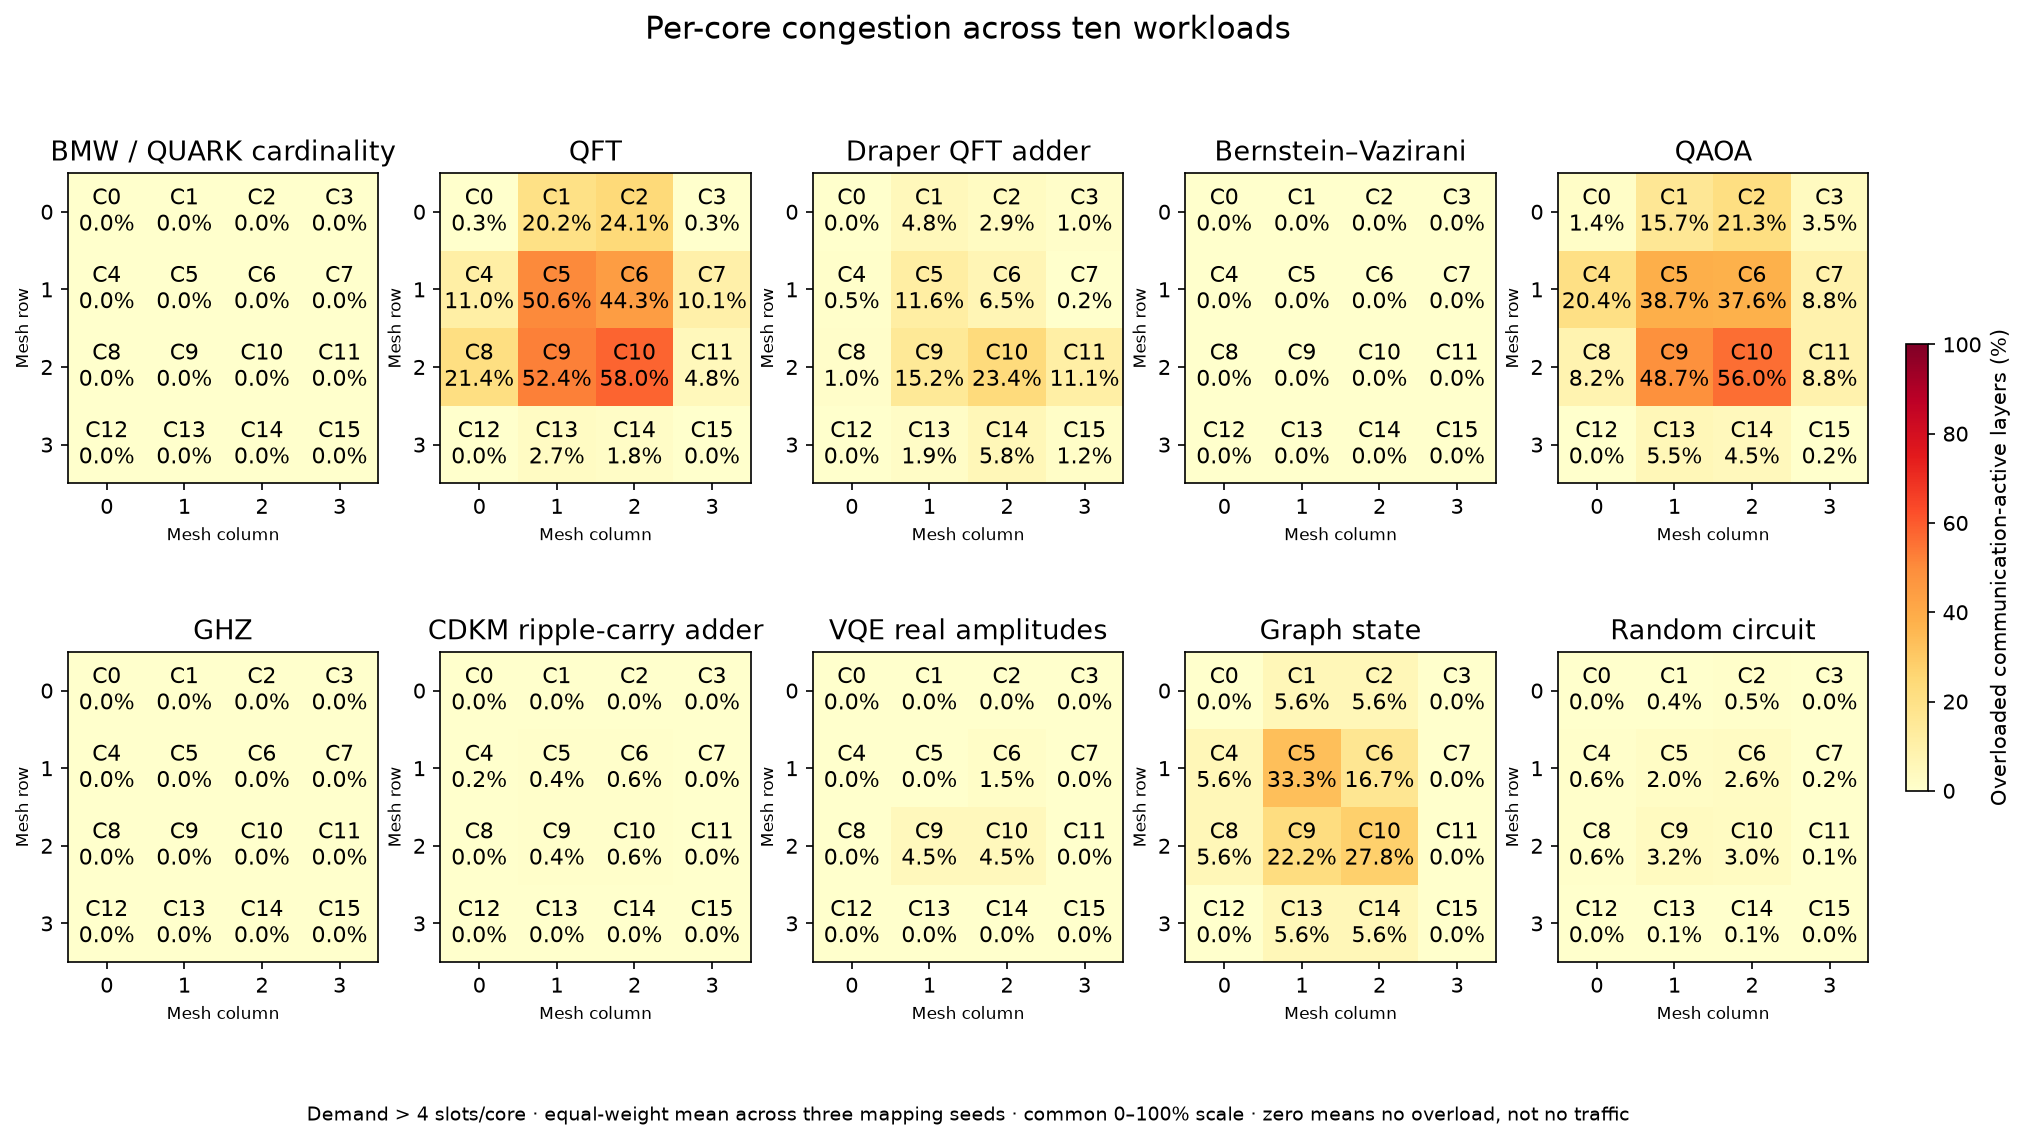
\includegraphics[width=\linewidth,height=0.80\textheight,keepaspectratio]{per_core_congestion.png}
\caption{Per-core congestion on the mesh: percentage of communication-active layers in which a core's demand exceeds 4 slots (mean over three mapping seeds). All 160 cells match the project's earlier figure at 0.1\% resolution.}
\label{fig:heatmap}
\end{figure}
\end{landscape}

\begin{table}[H]
\centering\small
\begin{tabular}{@{}lrrr@{}}
\toprule
Workload & Active layers (seeds 42/43/44) & Layers with any overload & Hottest core \\
\midrule
GHZ & 15/15/15 & 0.0\% & C0 (0.0\%) \\
Bernstein--Vazirani & 16/16/16 & 0.0\% & C0 (0.0\%) \\
BMW/QUARK cardinality & 90/90/90 & 0.0\% & C0 (0.0\%) \\
VQE real amplitudes & 22/22/22 & 6.1\% & C9 (4.5\%) \\
CDKM ripple-carry adder & 157/157/157 & 0.6\% & C6 (0.6\%) \\
Graph state & 6/6/6 & 33.3\% & C5 (33.3\%) \\
Draper QFT adder & 138/138/138 & 41.3\% & C10 (23.4\%) \\
QAOA & 163/163/163 & 71.6\% & C10 (56.0\%) \\
QFT & 112/112/112 & 65.2\% & C10 (58.0\%) \\
Random circuit & 2296/2296/2296 & 8.0\% & C9 (3.2\%) \\
\bottomrule
\end{tabular}
\caption{Structural overload at capacity 4, pooled over the three mapping seeds.}
\label{tab:heatmap}
\end{table}


Congestion concentrates on the central cores, which lie on the most shortest paths. QFT and QAOA are the heavy cases, graph state is
overloaded in a third of its (few) active layers, and GHZ, Bernstein--Vazirani and BMW never exceed four.

\section{Own demand against relay demand (Experiment 2)}
A \emph{route} is a qubit's consecutive hops within one layer; its first source and final destination are its \emph{endpoints}, every core in
between is a \emph{relay}. For a core and a layer, $D$ counts the hops touching the core, $D_{\mathrm{end}}$ those where the core is an endpoint of the
route, and $D_{\mathrm{relay}}$ the rest, so that a relay (touched by an arriving and a leaving hop) contributes two: $D=D_{\mathrm{end}}+D_{\mathrm{relay}}$.
With capacity $C$, a layer is overloaded for the core when $D>C$. It is \emph{own-overloaded} when $D_{\mathrm{end}}>C$, and \emph{relay-only-overloaded}
when $D_{\mathrm{end}}\le C<D$. The two sets are disjoint and together are exactly the overloaded layers.

\paragraph{Validation.} Own plus relay-only reproduces all 160 heatmap cells, and the per-core relay incidences, incident hops and peak layer demand reproduce
all 480 per-trial rows of the archive's per-core file exactly.

\paragraph{Counting qubits in flight.} A second variant counts routes instead of hops: under per-qubit ordering the hops of a route run one after
another, so a relay needs one memory for the route at a time, not two.


\begin{table}[H]
\centering\small
\resizebox{\ifdim\width>\linewidth\linewidth\else\width\fi}{!}{%
\begin{tabular}{@{}lrrrr@{}}
\toprule
Workload & C=1 & C=2 & C=3 & C=4 \\
\midrule
GHZ & 0.0\% & none & none & none \\
Bernstein--Vazirani & 0.0\% & none & none & none \\
BMW/QUARK cardinality & 0.0\% & none & none & none \\
VQE real amplitudes & 2.0\% & 0.0\% & 0.0\% & 0.0\% \\
CDKM ripple-carry adder & 0.4\% & 0.0\% & 0.0\% & 0.0\% \\
Graph state & 26.0\% & 9.5\% & 0.0\% & 0.0\% \\
Draper QFT adder & 54.5\% & 6.9\% & 6.4\% & 0.0\% \\
QAOA & 51.9\% & 14.9\% & 2.3\% & 0.4\% \\
QFT & 76.8\% & 10.1\% & 7.1\% & 0.0\% \\
Random circuit & 15.7\% & 1.8\% & 0.0\% & 0.0\% \\
\bottomrule
\end{tabular}}
\caption{Share of overloaded core-layers caused by a core's own endpoint demand (hop counting); the rest is relay-only overload.}
\label{tab:exp2-hop}
\end{table}

\begin{table}[H]
\centering\small
\begin{tabular}{@{}lrrrr@{}}
\toprule
Workload & C=1 & C=2 & C=3 & C=4 \\
\midrule
GHZ & none & none & none & none \\
Bernstein--Vazirani & none & none & none & none \\
BMW/QUARK cardinality & none & none & none & none \\
VQE real amplitudes & 5.3\% & 0.0\% & none & none \\
CDKM ripple-carry adder & 10.7\% & 0.0\% & 0.0\% & 0.0\% \\
Graph state & 37.5\% & 18.2\% & 0.0\% & 0.0\% \\
Draper QFT adder & 76.0\% & 9.5\% & 17.1\% & 0.0\% \\
QAOA & 59.7\% & 20.7\% & 4.5\% & 1.2\% \\
QFT & 86.8\% & 11.5\% & 12.8\% & 0.0\% \\
Random circuit & 39.6\% & 7.0\% & 0.0\% & 0.0\% \\
\bottomrule
\end{tabular}
\caption{Share of overloaded core-layers caused by a core's own endpoint demand (route counting); the rest is relay-only overload.}
\label{tab:exp2-route}
\end{table}


\begin{table}[H]
\centering\small
\resizebox{\ifdim\width>\linewidth\linewidth\else\width\fi}{!}{%
\begin{tabular}{@{}llrrrrr@{}}
\toprule
Workload & Hottest core & Overloaded \% & Own \% & Relay-only \% & Relay share of demand & Relay share of excess \\
\midrule
GHZ & none & 0.0 & 0.0 & 0.0 & -- & -- \\
Bernstein--Vazirani & none & 0.0 & 0.0 & 0.0 & -- & -- \\
BMW/QUARK cardinality & none & 0.0 & 0.0 & 0.0 & -- & -- \\
VQE real amplitudes & C9 & 4.5 & 0.0 & 4.5 & 80\% & 100\% \\
CDKM ripple-carry adder & C6 & 0.6 & 0.0 & 0.6 & 85\% & 100\% \\
Graph state & C5 & 33.3 & 0.0 & 33.3 & 93\% & 100\% \\
Draper QFT adder & C10 & 23.4 & 0.0 & 23.4 & 81\% & 100\% \\
QAOA & C10 & 56.0 & 0.0 & 56.0 & 81\% & 100\% \\
QFT & C10 & 58.0 & 0.0 & 58.0 & 78\% & 100\% \\
Random circuit & C9 & 3.2 & 0.0 & 3.2 & 87\% & 100\% \\
\bottomrule
\end{tabular}}
\caption{Hottest core of each workload at capacity 4 (hop counting): percentage of active layers overloaded, split into own and relay-only, and the relay share of its demand and of its excess.}
\label{tab:exp2-hottest}
\end{table}

\begin{table}[H]
\centering\small
\resizebox{\ifdim\width>\linewidth\linewidth\else\width\fi}{!}{%
\begin{tabular}{@{}lrrr@{}}
\toprule
Workload & Peak demand $D$ & Peak endpoint demand $D_{\mathrm{end}}$ & Peak routes through one core \\
\midrule
GHZ & 2 & 1 & 1 \\
Bernstein--Vazirani & 2 & 1 & 1 \\
BMW/QUARK cardinality & 2 & 1 & 1 \\
VQE real amplitudes & 5 & 2 & 3 \\
CDKM ripple-carry adder & 9 & 2 & 5 \\
Graph state & 13 & 3 & 7 \\
Draper QFT adder & 11 & 4 & 7 \\
QAOA & 18 & 5 & 10 \\
QFT & 24 & 4 & 13 \\
Random circuit & 12 & 3 & 6 \\
\bottomrule
\end{tabular}}
\caption{Peak demand at one core in one layer, over all mapping seeds: how close endpoint demand comes to the capacity.}
\label{tab:exp2-peaks}
\end{table}


\paragraph{Why the counting matters.} Hop counting charges a relay two touches (one arriving hop, one leaving hop), but under per-qubit ordering those two hops run one after the other, so a relay needs one memory at a time. Hop counting therefore overstates
contention, most visibly at one slot: GHZ is structurally ``overloaded'' at one slot by hop counting (20\% of its layers) yet never waits in the simulator, and route counting, whose peak for GHZ is one route per core, correctly shows no contention. This is why Experiment~1 relates the
simulated cost to the structure and why both counts are reported.

\paragraph{Findings.} At the modelled capacity of four, almost all overload is relay overload. The peak endpoint demand is 4 for QFT and Draper, 5 for QAOA and at most 3
for the others, against a total demand up to 24. The only own-overload at capacity 4 is in QAOA, at the corner cores C0 and C3 (0.61\% of active layers each), which is
0.44\% of QAOA's overload. Smaller budgets bring own demand in: QFT is 77\% own-overload at capacity 1. A routing change can therefore remove at most the relay part;
the own part is a floor set by the mapping. Route counting finds less overload than hop counting (core C10 of QFT is overloaded in 46.4\% of active layers against
58.0\%) and relay traffic is still essentially all of what remains.

\section{Every capacity, both countings}
Capacity four is the modelled value; the smaller capacities show how the split moves as memory is removed. Each of the following landscape pages shows one capacity and counting with every workload that has overload side by side: for each workload the left heatmap is the percentage of active layers in which the core is overloaded by its own endpoint demand and the right heatmap the percentage in which it is overloaded only because of relay traffic. Per-core numbers for capacities four and two are in Appendix~\ref{app:percore}; the data for all capacities and both countings are in \code{results/experiment2_own_vs_relay_2026-10-24/}.
\begin{landscape}
\begin{figure}[p]
\centering
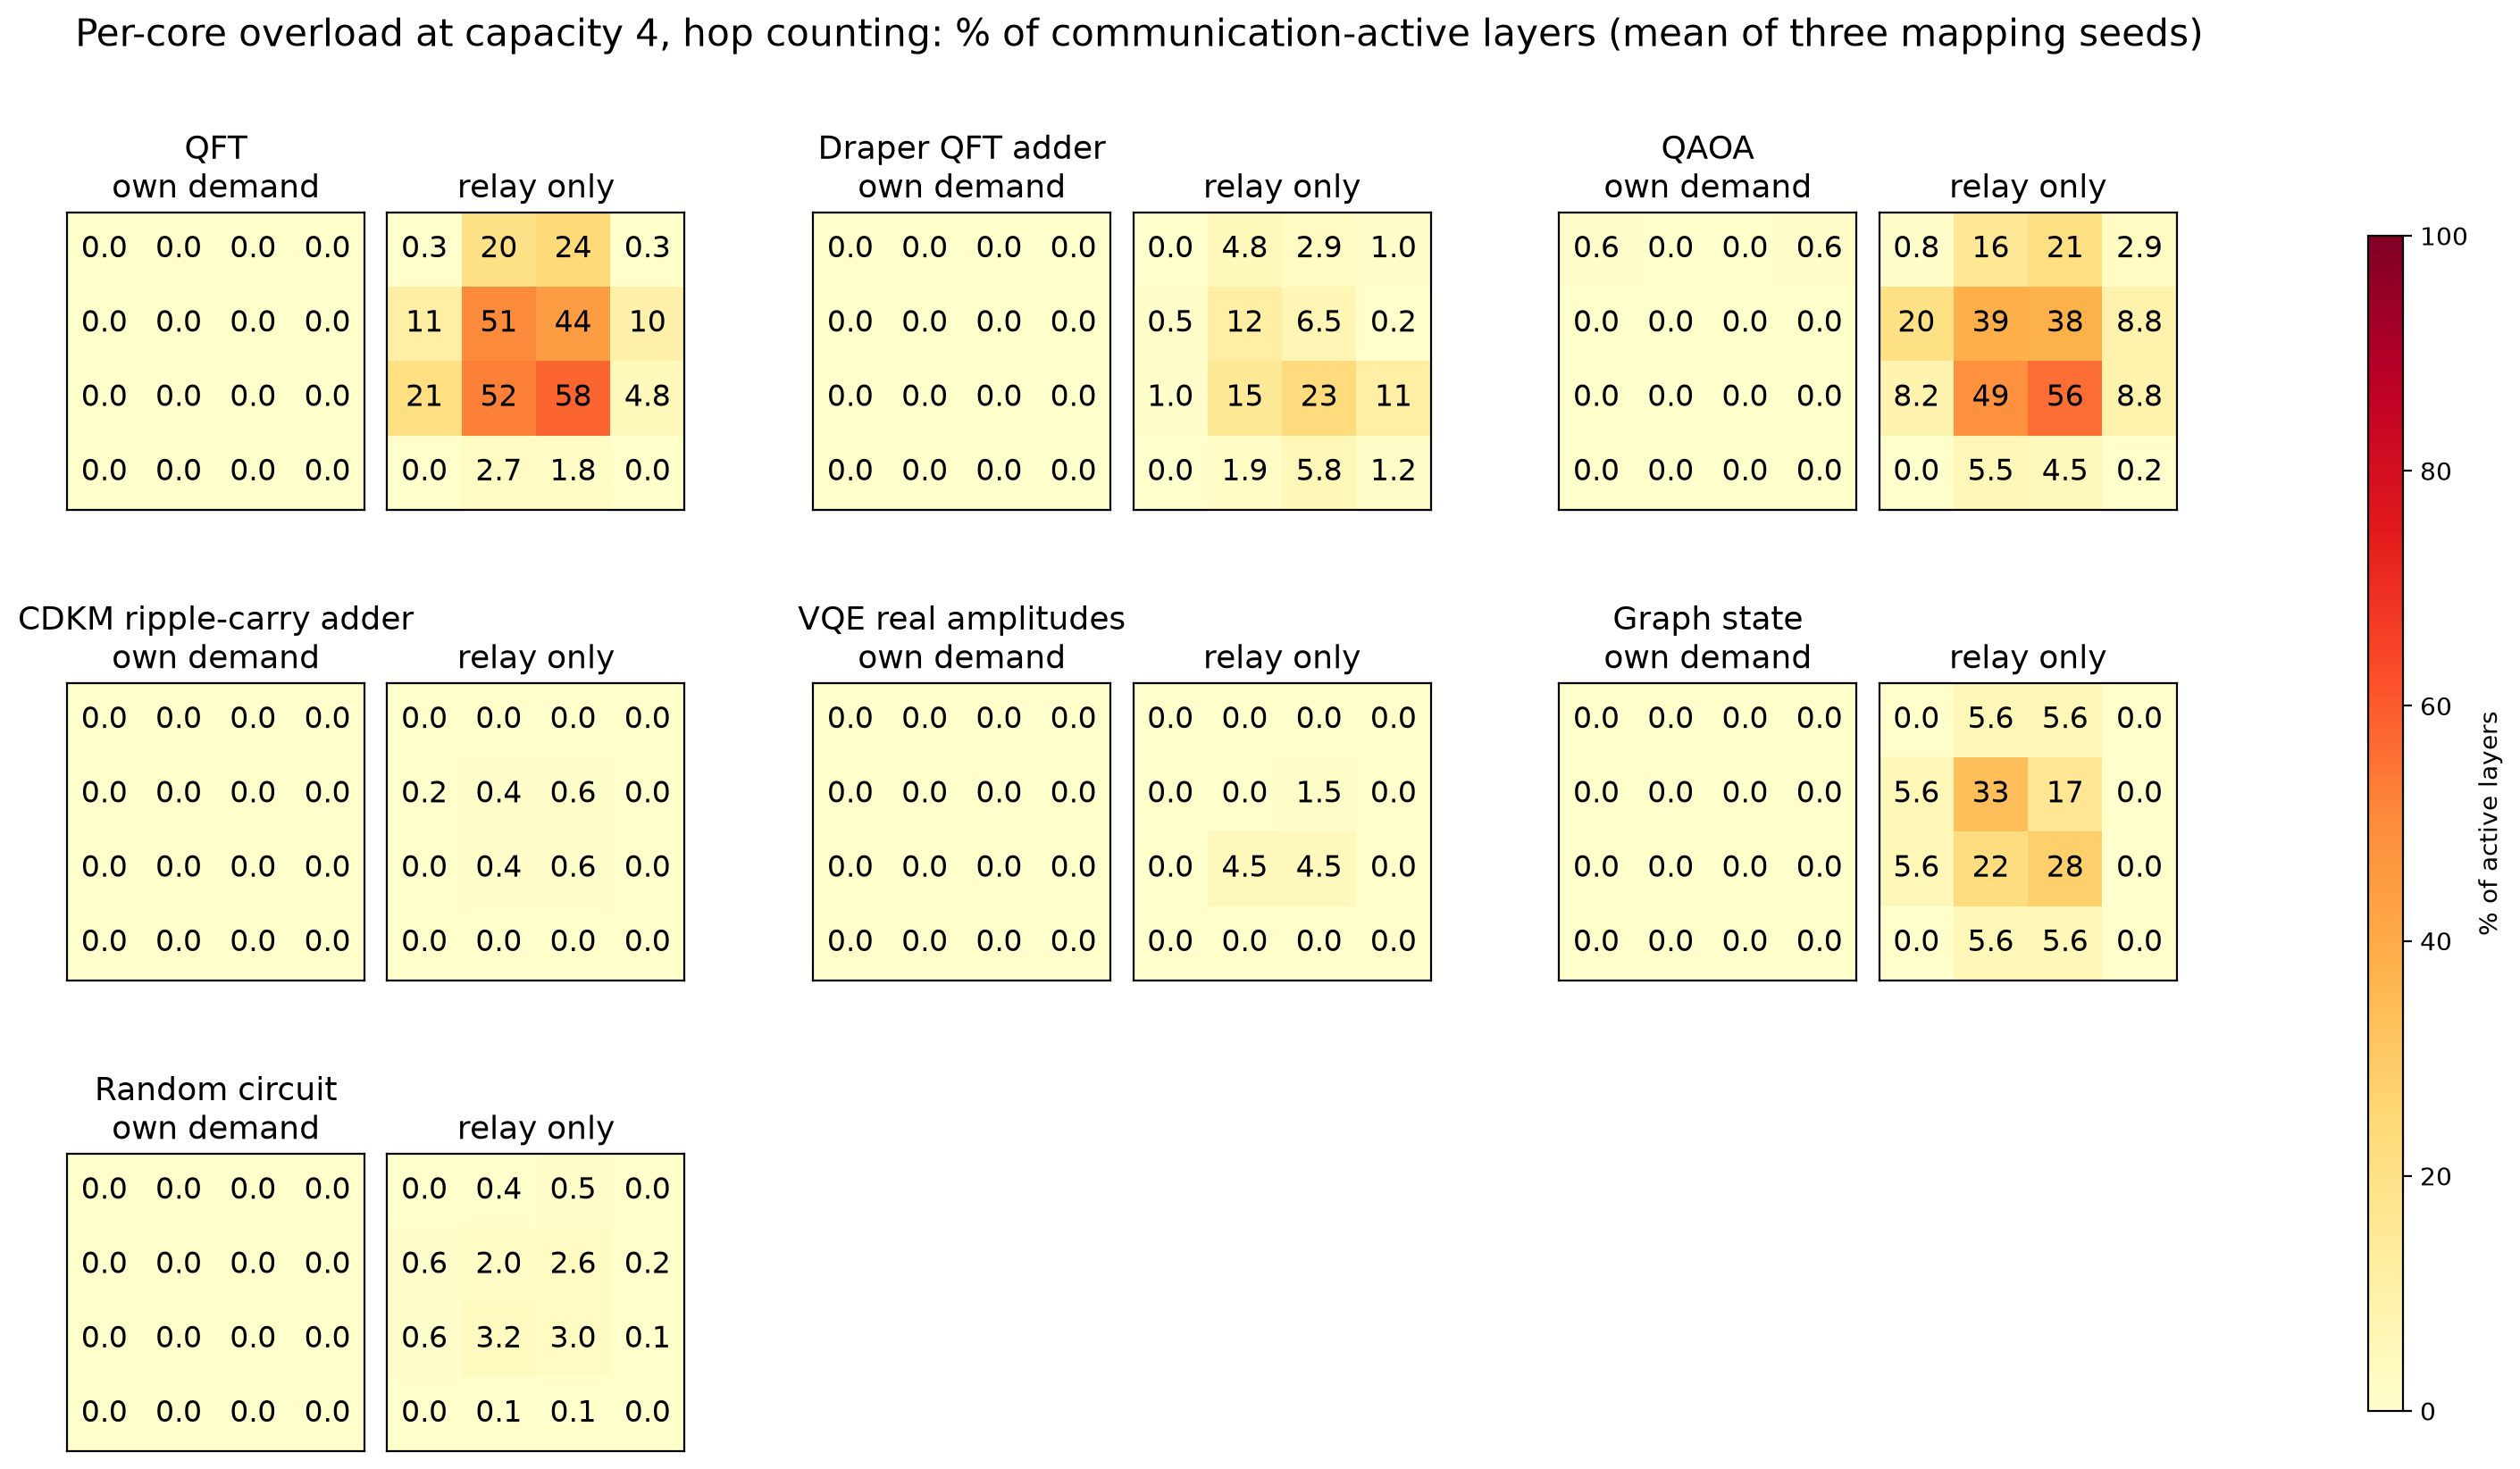
\includegraphics[width=\linewidth,height=0.80\textheight,keepaspectratio]{exp2_overview_c4_hop.png}
\caption{Capacity 4, hop counting. For each workload with overload, the left heatmap is the percentage of its active layers in which the core is overloaded by its own endpoint demand and the right heatmap the percentage in which it is overloaded only because of relay traffic. Mesh cores are numbered row by row (core 10 is row 2, column 2). Mean of three mapping seeds.}
\label{fig:exp2-overview-c4-hop}
\end{figure}
\end{landscape}
\begin{landscape}
\begin{figure}[p]
\centering
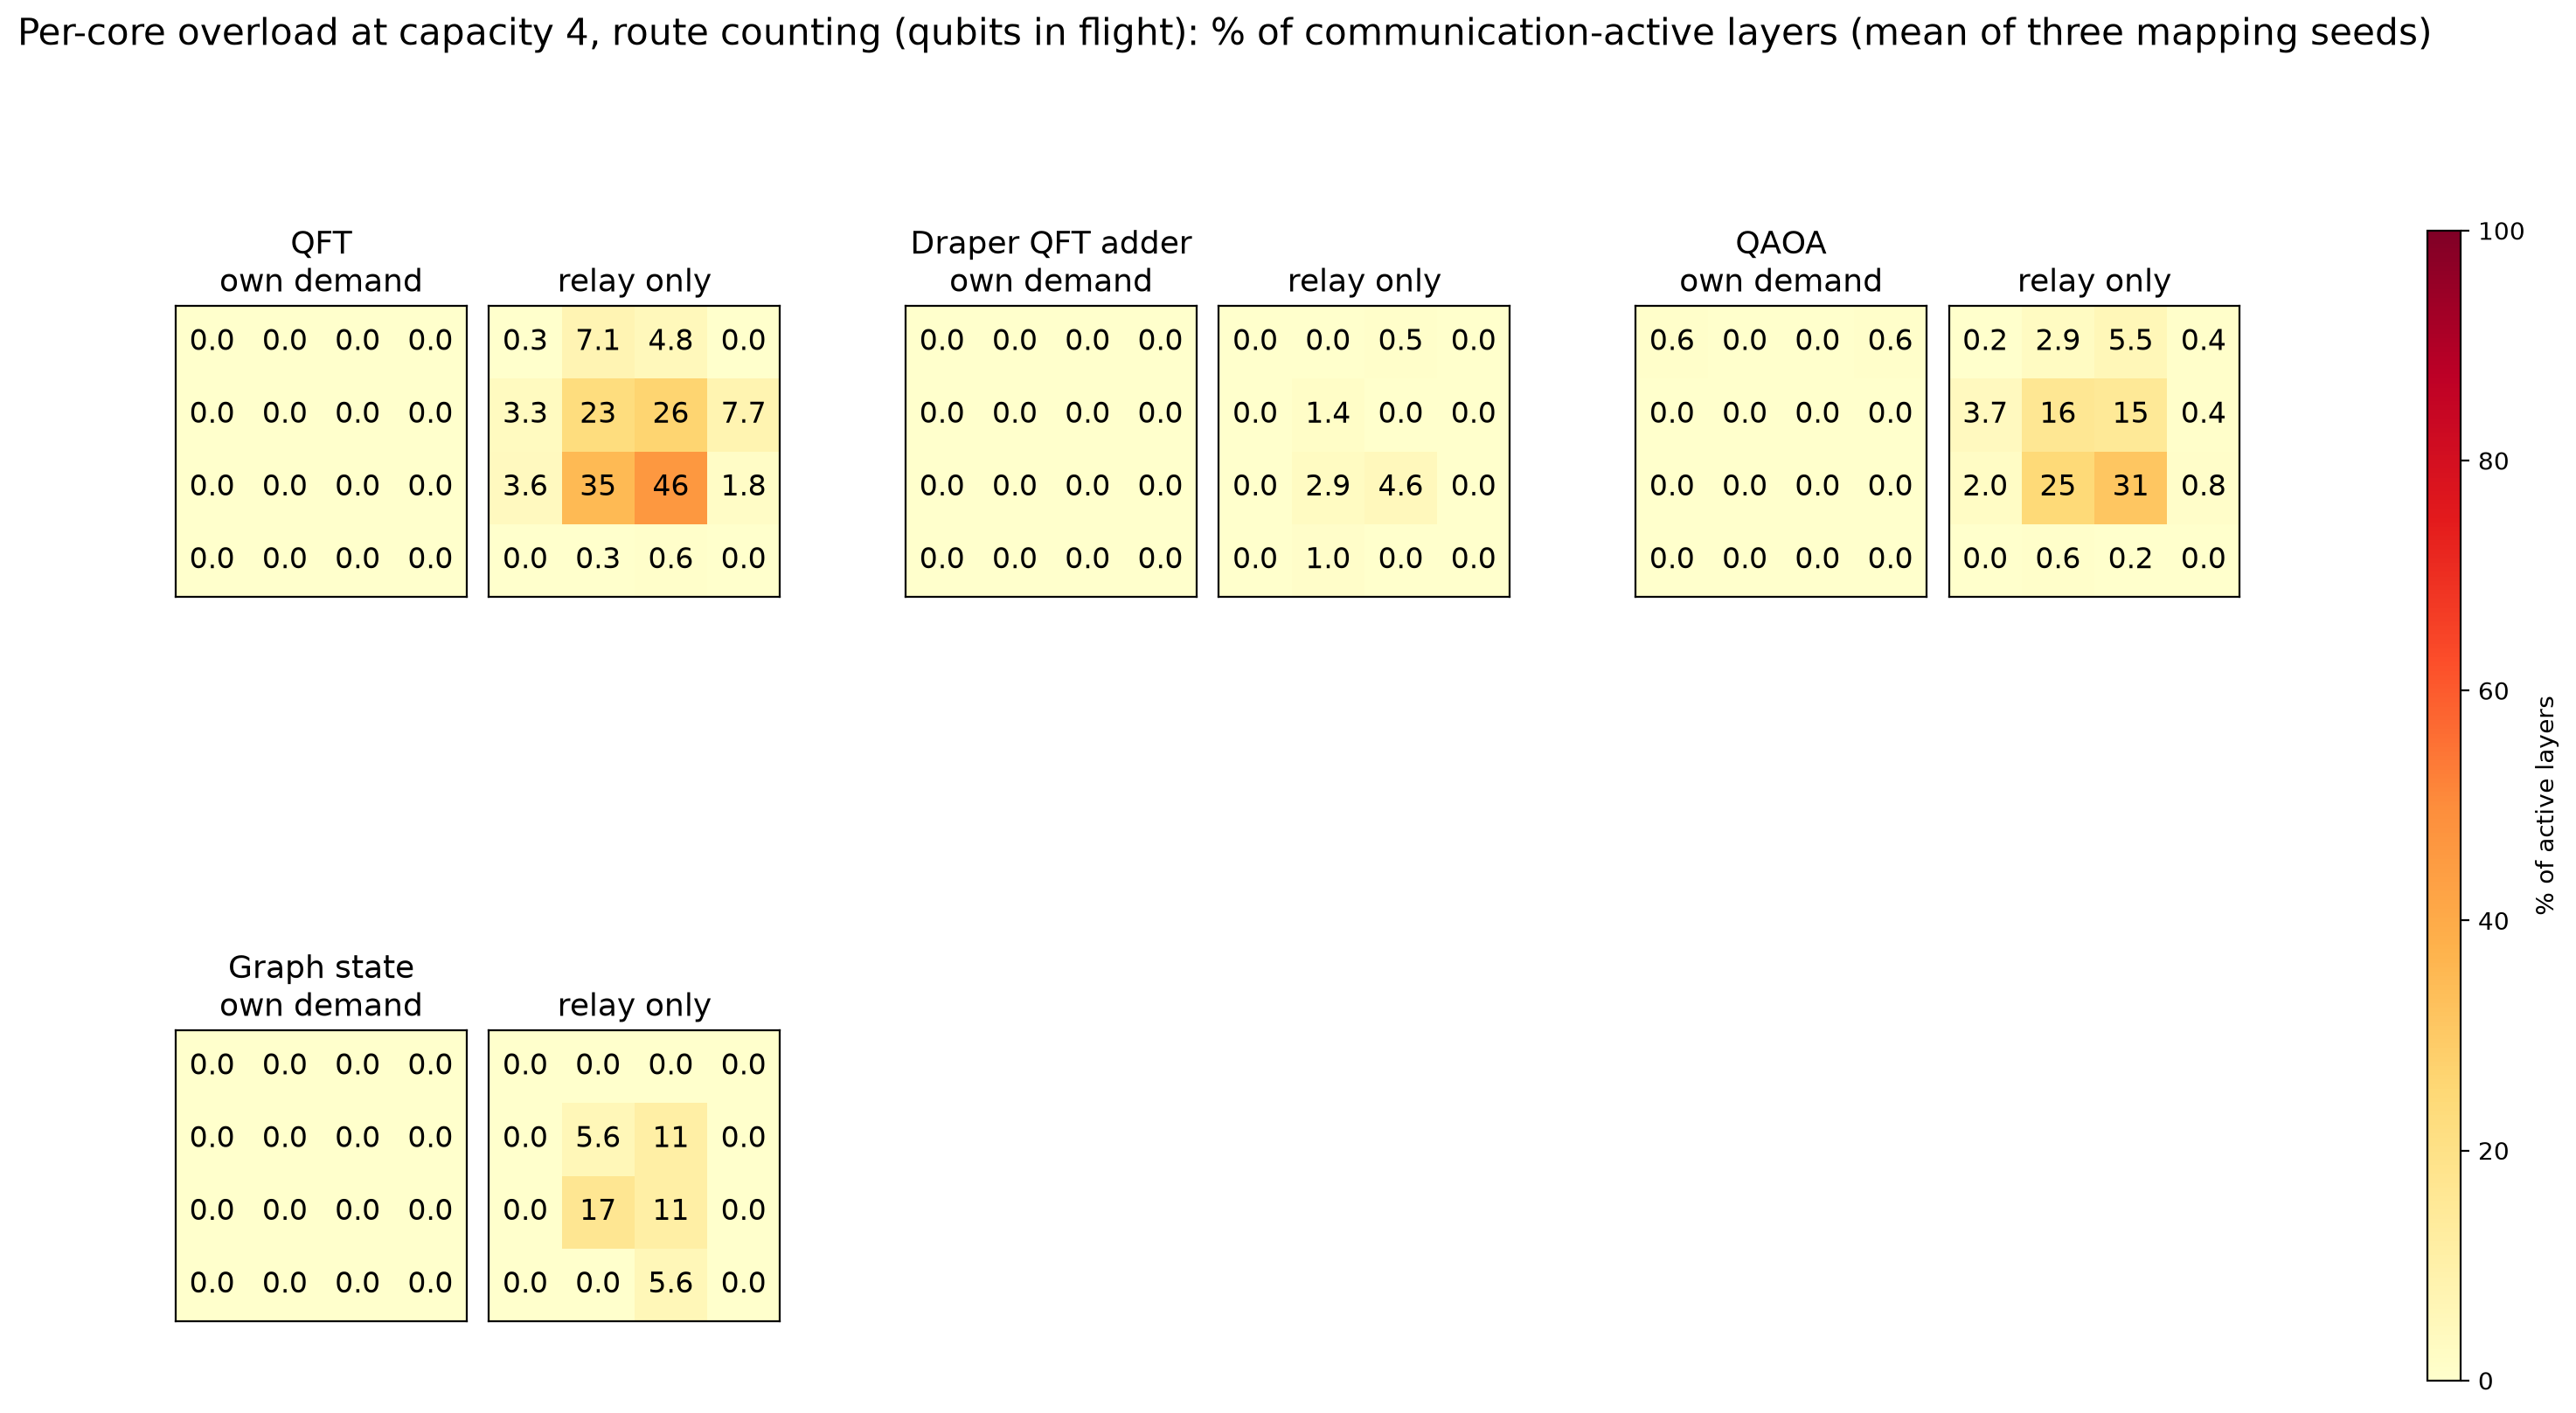
\includegraphics[width=\linewidth,height=0.80\textheight,keepaspectratio]{exp2_overview_c4_route.png}
\caption{Capacity 4, route counting (qubits in flight). For each workload with overload, the left heatmap is the percentage of its active layers in which the core is overloaded by its own endpoint demand and the right heatmap the percentage in which it is overloaded only because of relay traffic. Mesh cores are numbered row by row (core 10 is row 2, column 2). Mean of three mapping seeds.}
\label{fig:exp2-overview-c4-route}
\end{figure}
\end{landscape}
\begin{landscape}
\begin{figure}[p]
\centering
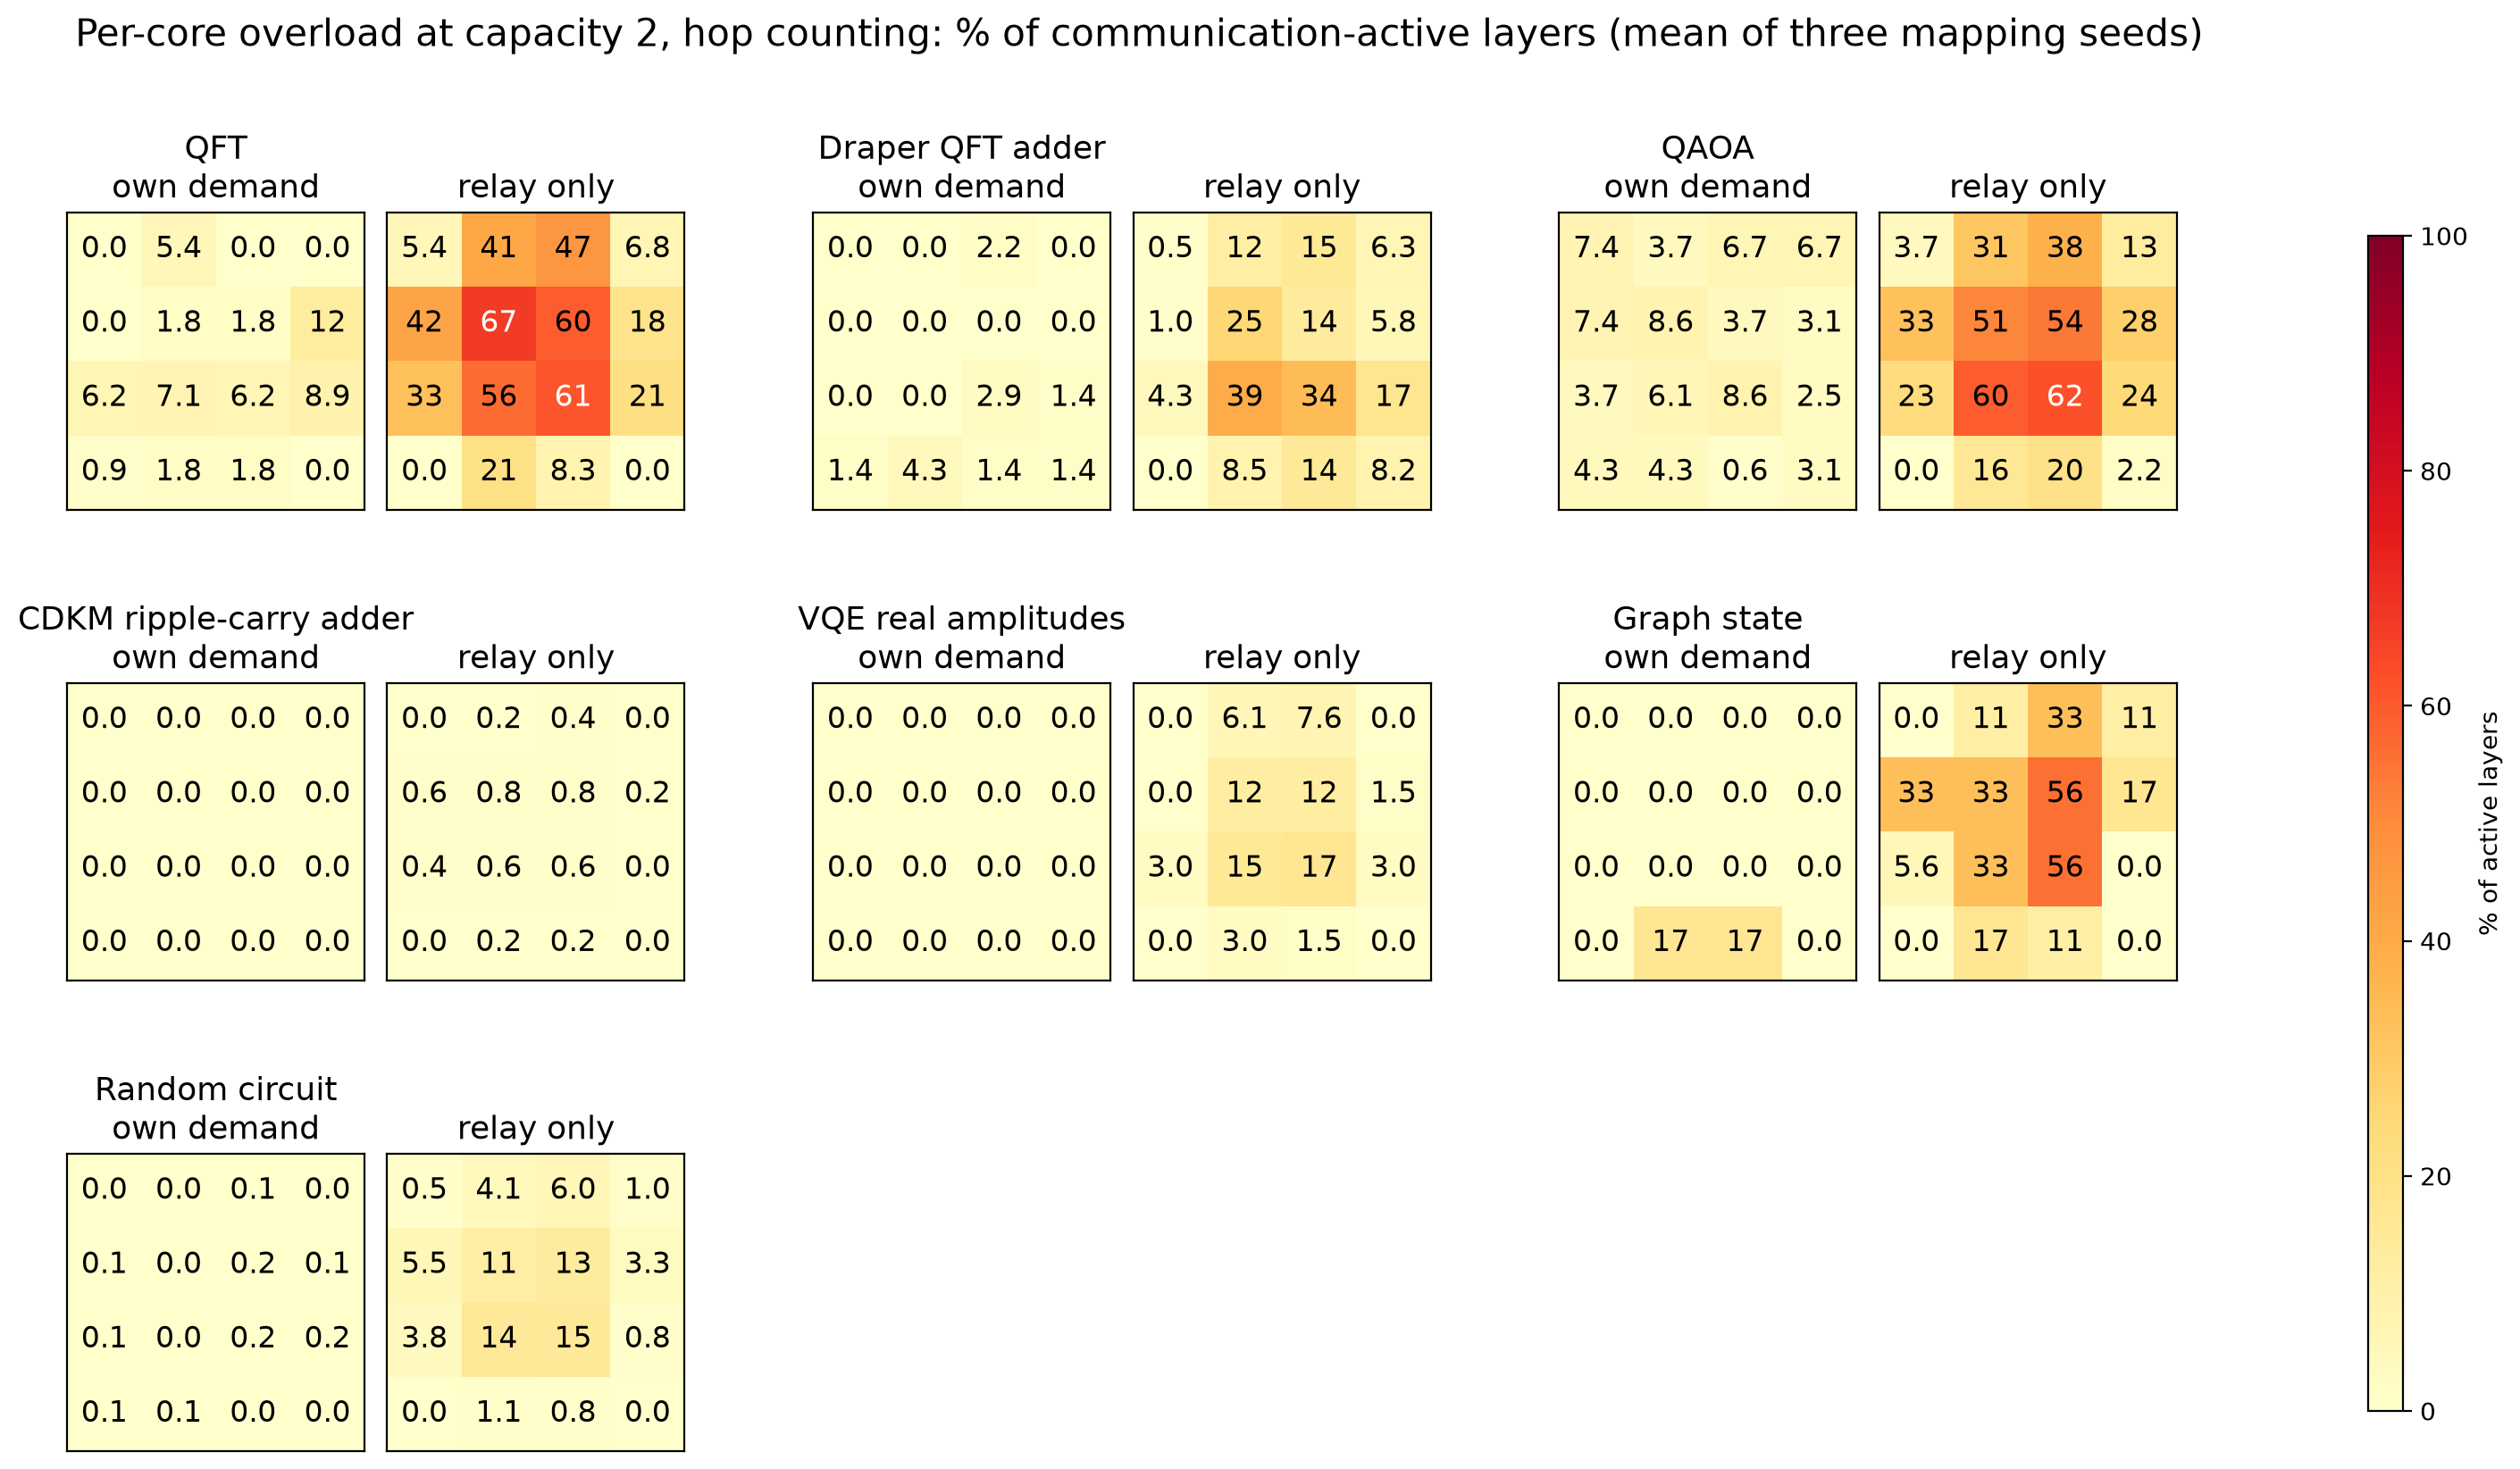
\includegraphics[width=\linewidth,height=0.80\textheight,keepaspectratio]{exp2_overview_c2_hop.png}
\caption{Capacity 2, hop counting. For each workload with overload, the left heatmap is the percentage of its active layers in which the core is overloaded by its own endpoint demand and the right heatmap the percentage in which it is overloaded only because of relay traffic. Mesh cores are numbered row by row (core 10 is row 2, column 2). Mean of three mapping seeds.}
\label{fig:exp2-overview-c2-hop}
\end{figure}
\end{landscape}
\begin{landscape}
\begin{figure}[p]
\centering
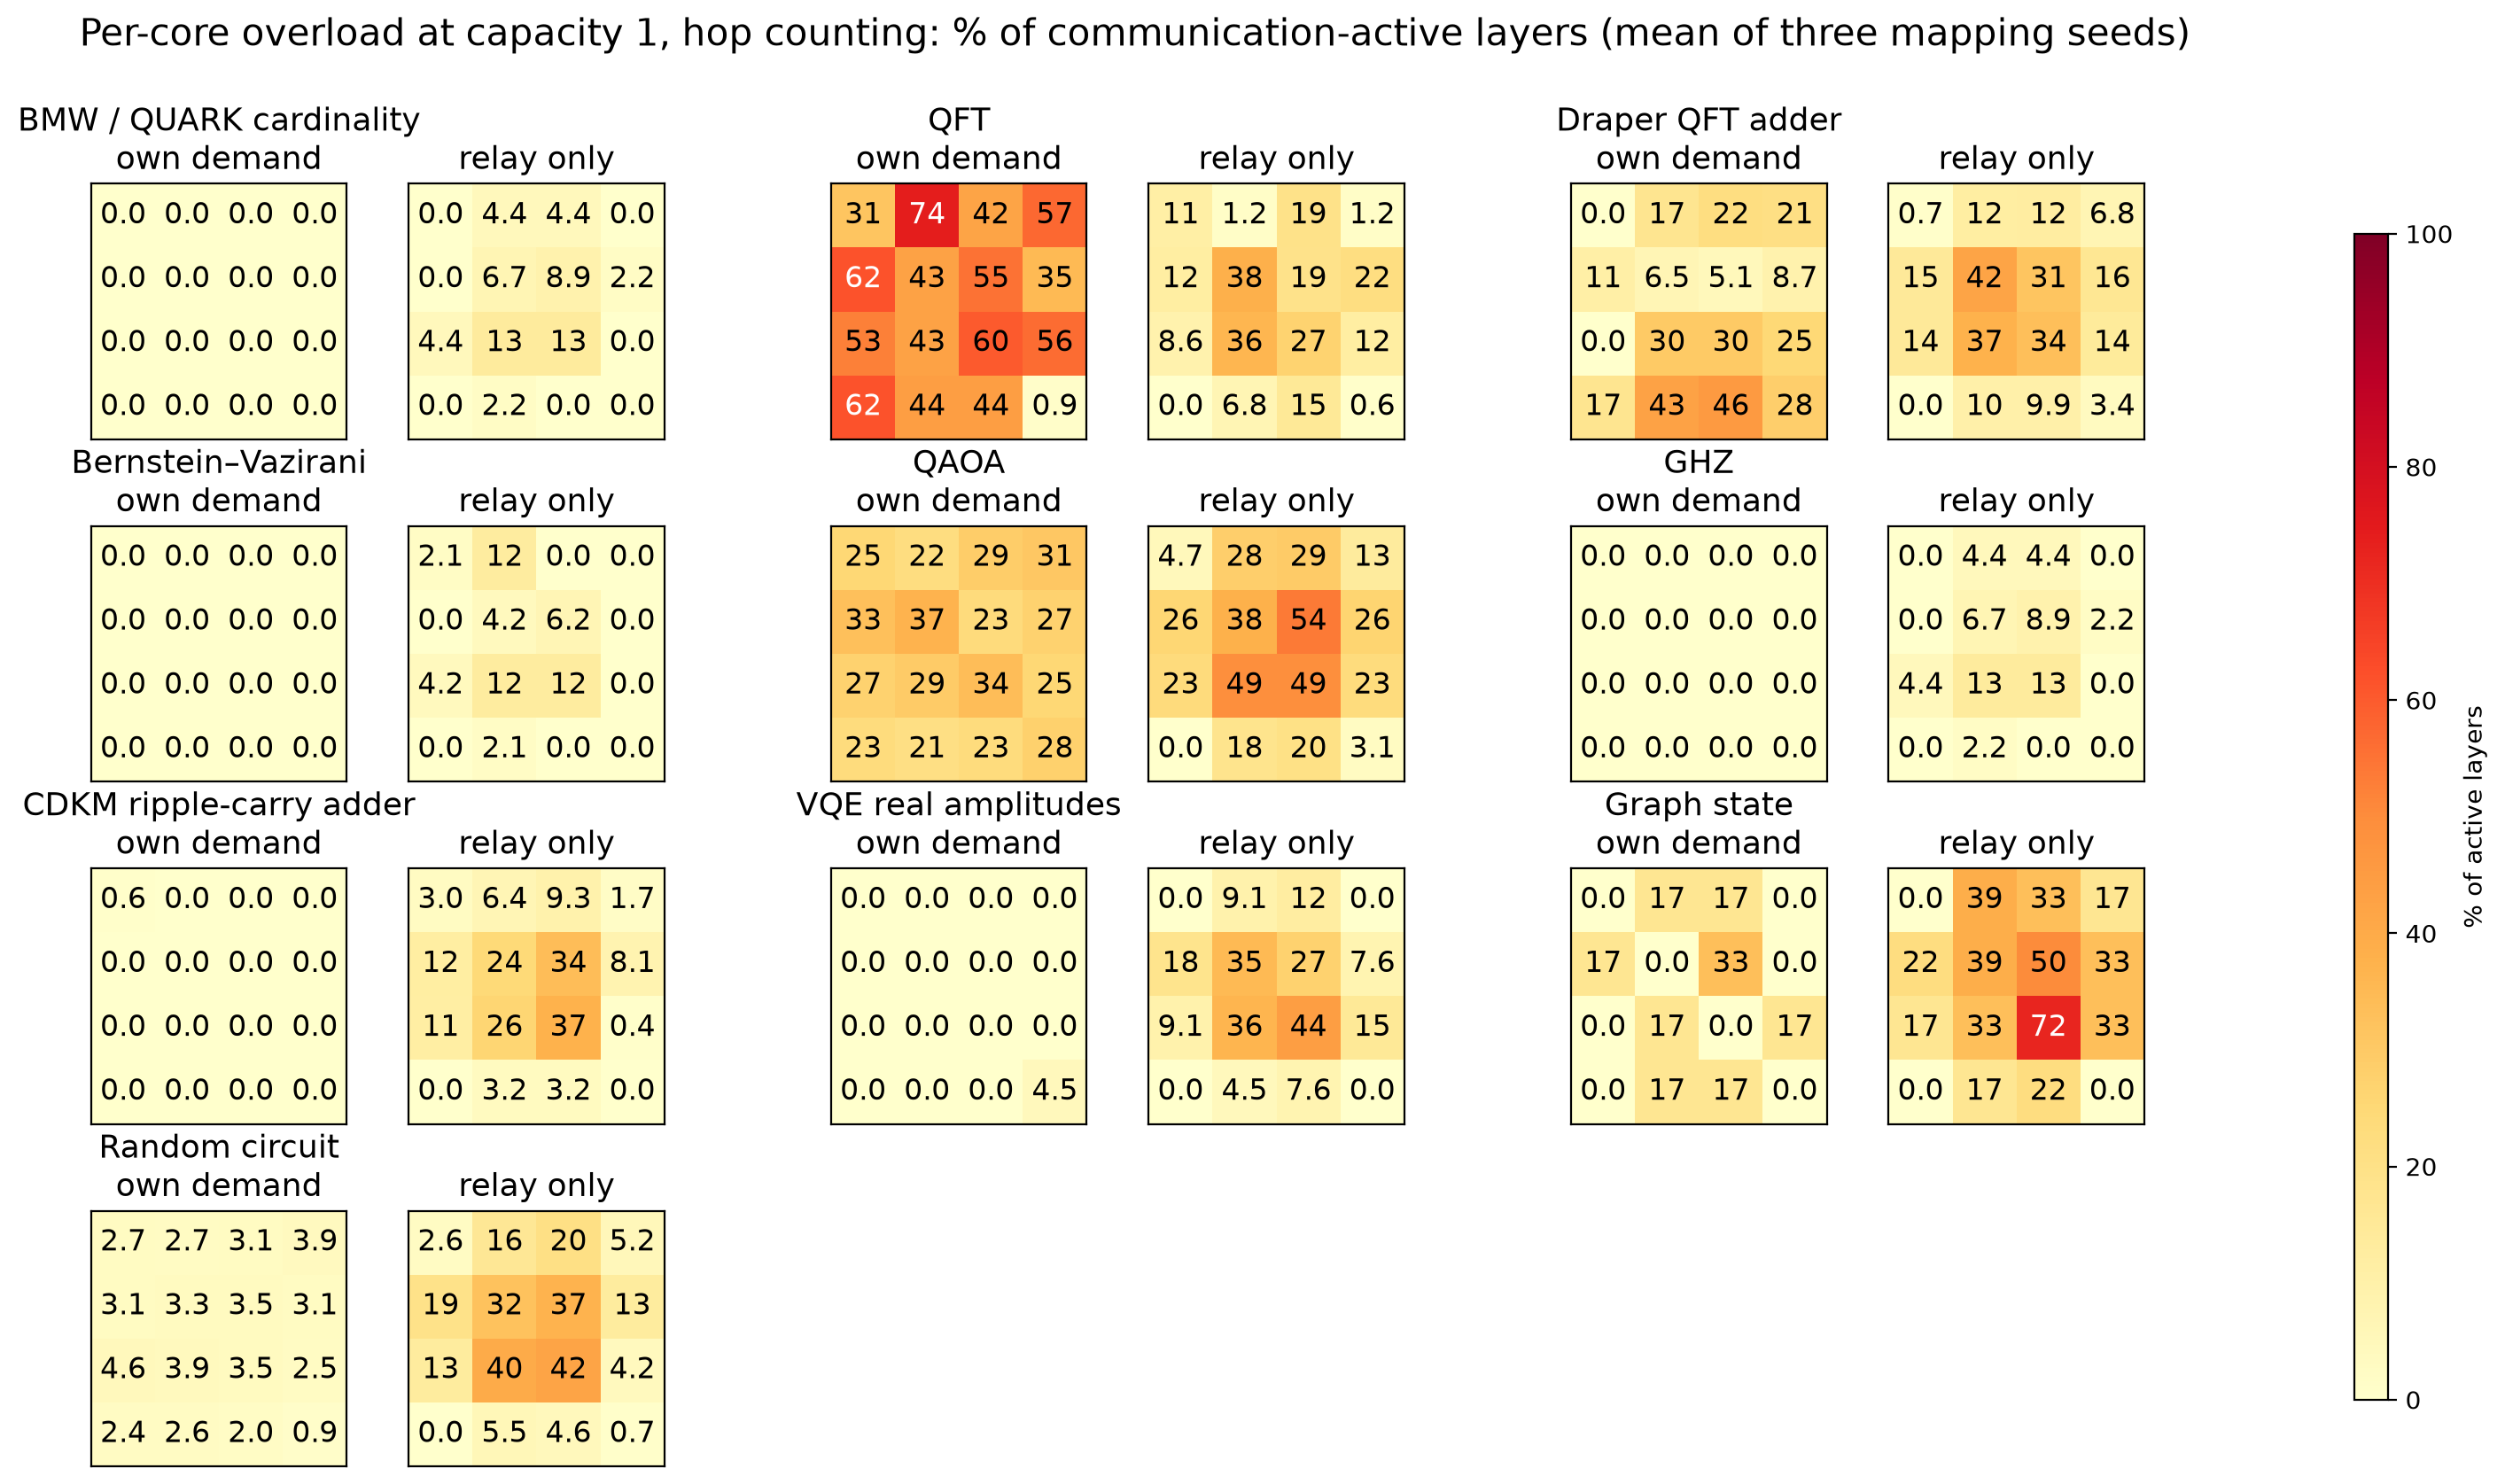
\includegraphics[width=\linewidth,height=0.80\textheight,keepaspectratio]{exp2_overview_c1_hop.png}
\caption{Capacity 1, hop counting. For each workload with overload, the left heatmap is the percentage of its active layers in which the core is overloaded by its own endpoint demand and the right heatmap the percentage in which it is overloaded only because of relay traffic. Mesh cores are numbered row by row (core 10 is row 2, column 2). Mean of three mapping seeds.}
\label{fig:exp2-overview-c1-hop}
\end{figure}
\end{landscape}
\begin{landscape}
\begin{figure}[p]
\centering
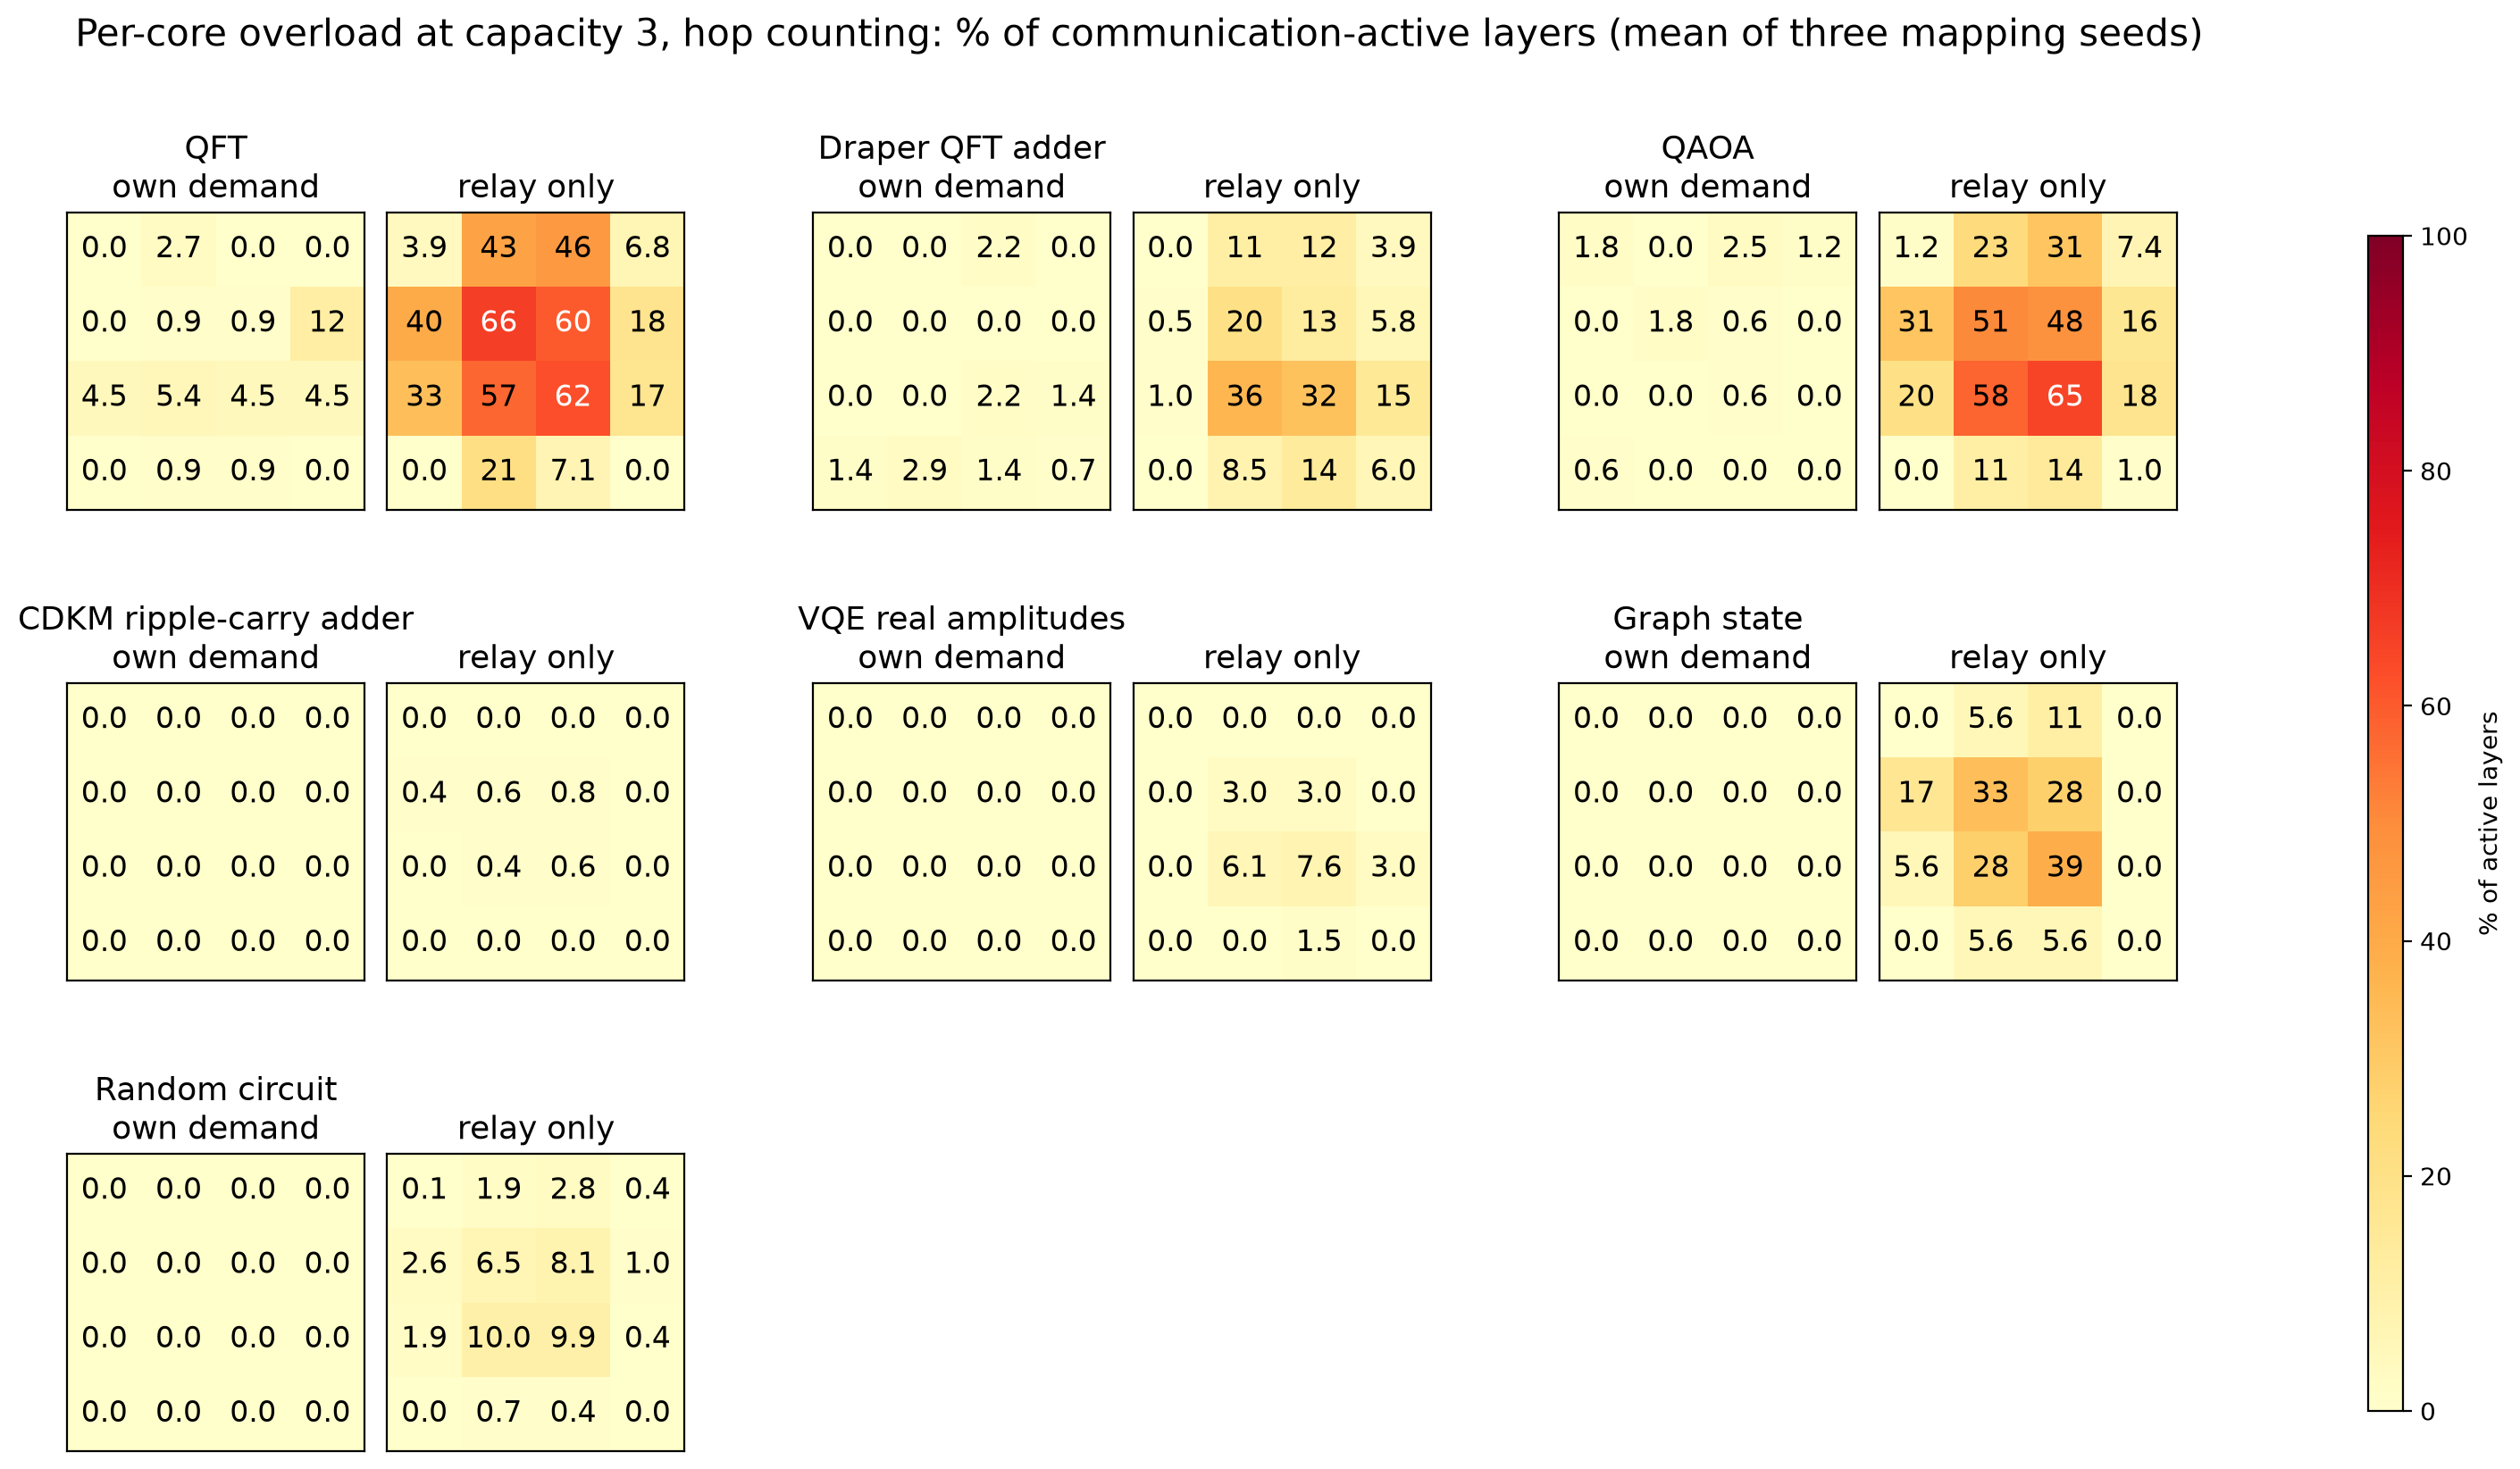
\includegraphics[width=\linewidth,height=0.80\textheight,keepaspectratio]{exp2_overview_c3_hop.png}
\caption{Capacity 3, hop counting. For each workload with overload, the left heatmap is the percentage of its active layers in which the core is overloaded by its own endpoint demand and the right heatmap the percentage in which it is overloaded only because of relay traffic. Mesh cores are numbered row by row (core 10 is row 2, column 2). Mean of three mapping seeds.}
\label{fig:exp2-overview-c3-hop}
\end{figure}
\end{landscape}


\chapter{Latency, fidelity and congestion across memory budgets (Experiment 1)}
\label{ch:exp1}

\section{Design}
All ten benchmarks, on the corrected scheduler, with $1,2,3,4,6,8,16,32$ communication memories per core (QFT also $64$). Budgets $1$--$4$ are \emph{modelled}
(the group's multi-core paper gives four communication qubits per core); $6$--$32$ are \emph{counterfactual} (what-if capacity), marked $^*$. Two policies:
\emph{on-demand} and \emph{dynamic} compiler pre-generation in which the compiler may hold at most $\text{budget}-1$ memories per core at once (the memories are one shared pool that any request can use; the cap limits only the compiler; dynamic starts at two memories because a cap of zero would be no pre-generation).
Three mapping seeds and three physics seeds give nine runs per cell, 1\,368 runs in total. Latency is the common latency defined in Chapter~\ref{ch:corrections}.

\section{Controls}
\begin{itemize}
  \item PASS every run completes every request: 1368 rows, 0 not ok
  \item PASS zero-congestion control: GHZ on-demand latency does not respond to the budget: 0 of 9 (mapping, physics) runs vary across budgets
  \item PASS saturation: QFT with 64 memories reproduces 32 run for run (relative 1e-6): 18 runs compared, largest relative difference 7.96e-12
  \item PASS on-demand delivered fidelity does not depend on the budget: 0 of 90 runs vary
  \item PASS on-demand latency does not rise when memory is added, beyond seed-to-seed noise: 639 budget steps: 1 rise by less than the physics-seed spread (largest 0.0005 ms), 0 rise by more
\end{itemize}

The first full run failed two controls for reasons that were not physical: the saturation check compared to exact equality although a few requests ``waited''
the one picosecond the scheduler leaves after a release, and one on-demand step rose by $0.0005$\,ms with more memory (a thirtieth of the seed-to-seed spread), which is sampling
noise because a delayed request draws different random numbers. The controls were refined, tests pin them, and a request now ``waited'' only if it waited more than a microsecond.
The rerun is numerically identical to the first run in every column except that redefined one, which also shows that the pipeline is deterministic.

\section{What congestion costs on-demand requests}
\begin{figure}[H]
\centering
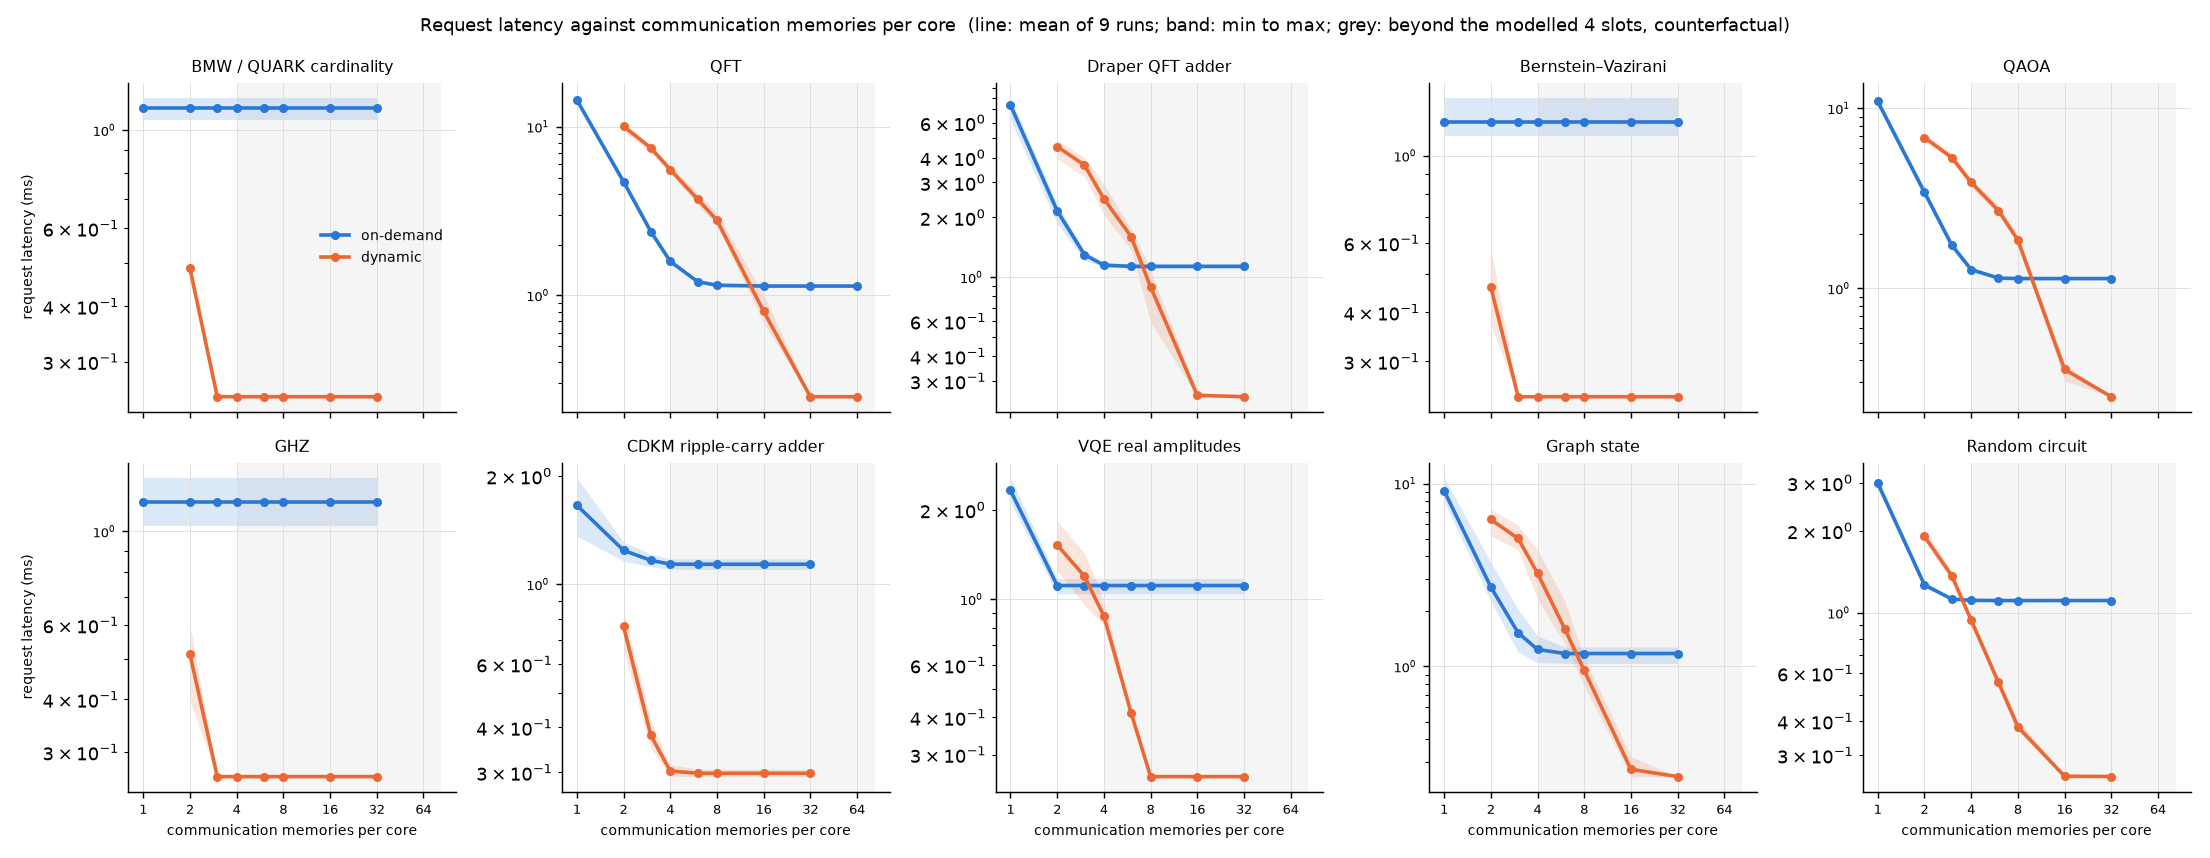
\includegraphics[width=\linewidth]{latency_vs_budget.png}
\caption{Request latency against communication memories per core. Line: mean of nine runs; band: minimum to maximum; grey: counterfactual budgets.}
\label{fig:exp1-latency}
\end{figure}

\begin{table}[H]
\centering\small
\resizebox{\ifdim\width>\linewidth\linewidth\else\width\fi}{!}{%
\begin{tabular}{@{}lrrrrrrrr@{}}
\toprule
Workload & 1 & 2 & 3 & 4 & 6$^*$ & 8$^*$ & 16$^*$ & 32$^*$ \\
\midrule
GHZ & 1.17$\pm$0.11 & 1.17$\pm$0.11 & 1.17$\pm$0.11 & 1.17$\pm$0.11 & 1.17$\pm$0.11 & 1.17$\pm$0.11 & 1.17$\pm$0.11 & 1.17$\pm$0.11 \\
Bernstein--Vazirani & 1.22$\pm$0.12 & 1.22$\pm$0.12 & 1.22$\pm$0.12 & 1.22$\pm$0.12 & 1.22$\pm$0.12 & 1.22$\pm$0.12 & 1.22$\pm$0.12 & 1.22$\pm$0.12 \\
BMW/QUARK cardinality & 1.12$\pm$0.04 & 1.12$\pm$0.04 & 1.12$\pm$0.04 & 1.12$\pm$0.04 & 1.12$\pm$0.04 & 1.12$\pm$0.04 & 1.12$\pm$0.04 & 1.12$\pm$0.04 \\
VQE real amplitudes & 2.32$\pm$0.14 & 1.11$\pm$0.05 & 1.11$\pm$0.05 & 1.11$\pm$0.05 & 1.11$\pm$0.05 & 1.11$\pm$0.05 & 1.11$\pm$0.05 & 1.11$\pm$0.05 \\
CDKM ripple-carry adder & 1.66$\pm$0.22 & 1.24$\pm$0.05 & 1.17$\pm$0.03 & 1.14$\pm$0.03 & 1.14$\pm$0.03 & 1.14$\pm$0.03 & 1.14$\pm$0.03 & 1.14$\pm$0.03 \\
Graph state & 9.14$\pm$1.14 & 2.72$\pm$0.54 & 1.53$\pm$0.30 & 1.24$\pm$0.13 & 1.18$\pm$0.08 & 1.18$\pm$0.08 & 1.18$\pm$0.08 & 1.18$\pm$0.08 \\
Draper QFT adder & 7.36$\pm$0.84 & 2.16$\pm$0.20 & 1.30$\pm$0.05 & 1.15$\pm$0.02 & 1.13$\pm$0.02 & 1.13$\pm$0.02 & 1.13$\pm$0.02 & 1.13$\pm$0.02 \\
QAOA & 10.92$\pm$0.41 & 3.42$\pm$0.14 & 1.74$\pm$0.06 & 1.27$\pm$0.02 & 1.14$\pm$0.01 & 1.13$\pm$0.01 & 1.13$\pm$0.01 & 1.13$\pm$0.01 \\
QFT & 14.42$\pm$0.35 & 4.72$\pm$0.14 & 2.39$\pm$0.09 & 1.59$\pm$0.05 & 1.21$\pm$0.02 & 1.15$\pm$0.02 & 1.13$\pm$0.02 & 1.13$\pm$0.02 \\
Random circuit & 2.99$\pm$0.10 & 1.27$\pm$0.02 & 1.12$\pm$0.01 & 1.11$\pm$0.01 & 1.11$\pm$0.01 & 1.11$\pm$0.01 & 1.11$\pm$0.01 & 1.11$\pm$0.01 \\
\bottomrule
\end{tabular}}
\caption{Request latency (ms), on-demand, mean $\pm$ sd over nine runs. Budgets marked $^*$ are counterfactual (beyond the modelled four slots).}
\label{tab:exp1-latency-ondemand}
\end{table}

Three workloads with no overload (GHZ, Bernstein--Vazirani, BMW) do not respond to the budget at all. At one memory the congested workloads are severe: QFT is about 12.7 times
its saturated latency, QAOA 9.6, graph state 7.8 and Draper 6.5. At the modelled four memories the penalty against 32 memories is $+40\%$ for QFT, $+12\%$ for QAOA, $+5\%$ for graph state and
$+1\%$ for Draper; the other workloads are within a percent. The floor, reached once nothing waits, is $1.11$ to $1.22$\,ms in every workload: that is generation time, not contention.

\begin{table}[H]
\centering\small
\resizebox{\ifdim\width>\linewidth\linewidth\else\width\fi}{!}{%
\begin{tabular}{@{}lrrrrrr@{}}
\toprule
Workload & 1 & 2 & 3 & 4 & 6$^*$ & 8$^*$ \\
\midrule
GHZ & +0\% & +0\% & +0\% & +0\% & +0\% & +0\% \\
Bernstein--Vazirani & +0\% & +0\% & +0\% & +0\% & +0\% & +0\% \\
BMW/QUARK cardinality & +0\% & +0\% & +0\% & +0\% & +0\% & +0\% \\
VQE real amplitudes & +109\% & +0\% & +0\% & +0\% & +0\% & +0\% \\
CDKM ripple-carry adder & +46\% & +9\% & +3\% & +0\% & +0\% & +0\% \\
Graph state & +676\% & +131\% & +30\% & +5\% & +0\% & +0\% \\
Draper QFT adder & +549\% & +90\% & +14\% & +1\% & +0\% & +0\% \\
QAOA & +863\% & +202\% & +53\% & +12\% & +1\% & -0\% \\
QFT & +1170\% & +316\% & +110\% & +40\% & +6\% & +1\% \\
Random circuit & +170\% & +14\% & +1\% & +0\% & +0\% & +0\% \\
\bottomrule
\end{tabular}}
\caption{On-demand latency relative to the same workload with 32 memories (saturated), by memories per core. $^*$ counterfactual.}
\label{tab:exp1-penalty}
\end{table}

\begin{table}[H]
\centering\small
\resizebox{\ifdim\width>\linewidth\linewidth\else\width\fi}{!}{%
\begin{tabular}{@{}lrrrrrrrrr@{}}
\toprule
Workload & OD 1 & OD 2 & OD 4 & OD 8 & OD 32 & Dyn 2 & Dyn 4 & Dyn 8 & Dyn 32 \\
\midrule
GHZ & 0.33 & 0.33 & 0.33 & 0.33 & 0.33 & 0.31 & 0.30 & 0.30 & 0.30 \\
Bernstein--Vazirani & 0.89 & 0.89 & 0.89 & 0.89 & 0.89 & 0.87 & 0.86 & 0.86 & 0.86 \\
BMW/QUARK cardinality & 6.95 & 6.95 & 6.95 & 6.95 & 6.95 & 6.86 & 6.83 & 6.83 & 6.83 \\
VQE real amplitudes & 0.74 & 0.68 & 0.68 & 0.68 & 0.68 & 0.68 & 0.63 & 0.61 & 0.61 \\
CDKM ripple-carry adder & 5.62 & 5.59 & 5.58 & 5.58 & 5.58 & 5.37 & 5.20 & 5.20 & 5.20 \\
Graph state & 0.38 & 0.26 & 0.24 & 0.24 & 0.24 & 0.32 & 0.26 & 0.23 & 0.22 \\
Draper QFT adder & 6.89 & 5.14 & 4.88 & 4.87 & 4.87 & 5.91 & 5.03 & 4.54 & 4.41 \\
QAOA & 10.69 & 6.60 & 5.48 & 5.40 & 5.40 & 8.50 & 6.62 & 5.52 & 4.74 \\
QFT & 9.11 & 5.72 & 4.66 & 4.51 & 4.51 & 7.50 & 5.75 & 4.79 & 4.05 \\
Random circuit & 59.78 & 51.50 & 50.89 & 50.89 & 50.89 & 53.58 & 47.74 & 45.05 & 44.58 \\
\bottomrule
\end{tabular}}
\caption{Makespan (simulated seconds of the whole circuit), on-demand (OD) and dynamic (Dyn), by memories per core. Mostly the fixed 5.3\,ms lead and 5\,ms empty-layer gap.}
\label{tab:exp1-makespan}
\end{table}

\begin{table}[H]
\centering\small
\resizebox{\ifdim\width>\linewidth\linewidth\else\width\fi}{!}{%
\begin{tabular}{@{}lrrrrrr@{}}
\toprule
Workload & 2 mem. seed 42 & 43 & 44 & 4 mem. seed 42 & 43 & 44 \\
\midrule
GHZ & 1.21 & 1.13 & 1.18 & 1.21 & 1.13 & 1.18 \\
Bernstein--Vazirani & 1.24 & 1.22 & 1.21 & 1.24 & 1.22 & 1.21 \\
BMW/QUARK cardinality & 1.11 & 1.13 & 1.11 & 1.11 & 1.13 & 1.11 \\
VQE real amplitudes & 1.15 & 1.11 & 1.08 & 1.15 & 1.11 & 1.08 \\
CDKM ripple-carry adder & 1.26 & 1.28 & 1.18 & 1.14 & 1.13 & 1.14 \\
Graph state & 2.42 & 2.33 & 3.41 & 1.19 & 1.16 & 1.36 \\
Draper QFT adder & 2.26 & 1.89 & 2.32 & 1.16 & 1.14 & 1.15 \\
QAOA & 3.59 & 3.39 & 3.28 & 1.28 & 1.29 & 1.25 \\
QFT & 4.60 & 4.91 & 4.66 & 1.57 & 1.65 & 1.55 \\
Random circuit & 1.28 & 1.27 & 1.24 & 1.11 & 1.11 & 1.11 \\
\bottomrule
\end{tabular}}
\caption{On-demand latency (ms) by mapping seed (mean over the three physics seeds): where there is congestion the mapping seed matters more than the physics seed; where nothing waits the physics noise dominates.}
\label{tab:exp1-mapseed}
\end{table}

The makespan is dominated by the fixed $5.3$\,ms lead and $5$\,ms empty-layer gap, so it moves much less than the request latency. Where there is congestion the spread between mapping seeds is several times the spread between physics seeds at two memories (graph state: $0.60$\,ms between the three mapping-seed means against $0.15$\,ms between physics seeds; Draper: $0.23$ against $0.02$); where nothing waits the physics noise dominates. Over the 20 workload-and-budget cells of Table~\ref{tab:exp1-mapseed} the mapping spread is the larger in 9.

\section{Congestion as waiting}
\begin{figure}[H]
\centering
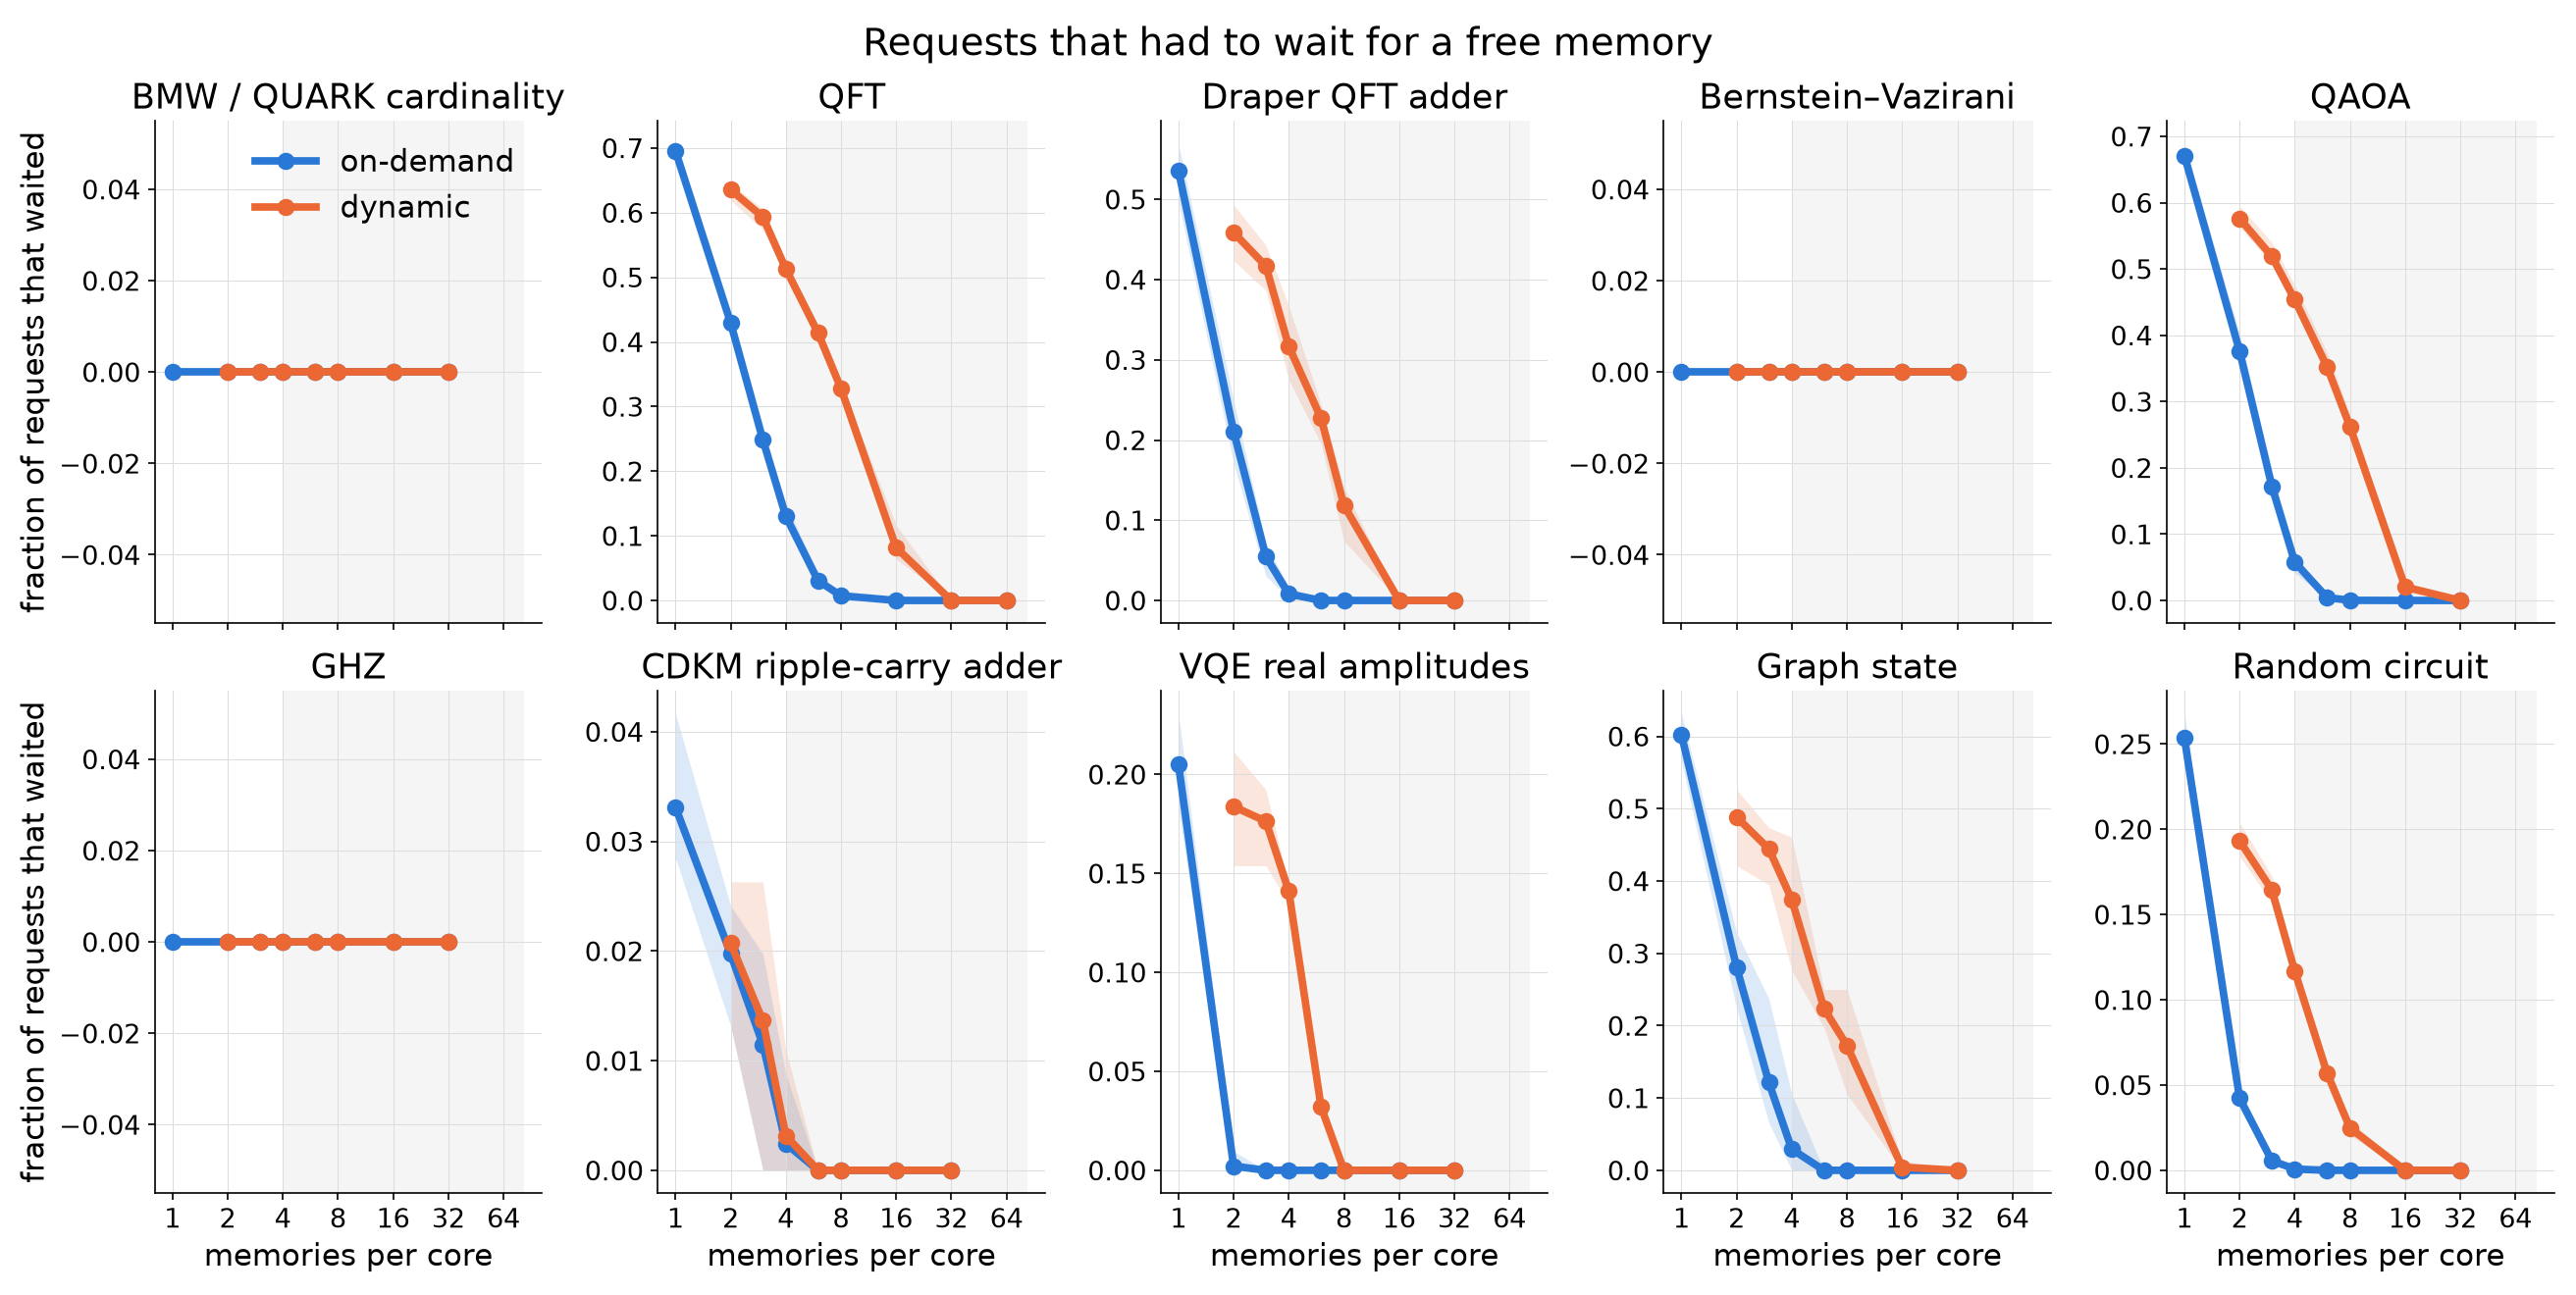
\includegraphics[width=\linewidth]{waiting_vs_budget.png}
\caption{Fraction of requests that had to wait for a free memory. Line: mean of nine runs; band: minimum to maximum; grey: counterfactual budgets.}
\label{fig:exp1-waiting}
\end{figure}

\begin{table}[H]
\centering\small
\resizebox{\ifdim\width>\linewidth\linewidth\else\width\fi}{!}{%
\begin{tabular}{@{}lrrrrrrrr@{}}
\toprule
Workload & 1 & 2 & 3 & 4 & 6$^*$ & 8$^*$ & 16$^*$ & 32$^*$ \\
\midrule
GHZ & 0.000 & 0.000 & 0.000 & 0.000 & 0.000 & 0.000 & 0.000 & 0.000 \\
Bernstein--Vazirani & 0.000 & 0.000 & 0.000 & 0.000 & 0.000 & 0.000 & 0.000 & 0.000 \\
BMW/QUARK cardinality & 0.000 & 0.000 & 0.000 & 0.000 & 0.000 & 0.000 & 0.000 & 0.000 \\
VQE real amplitudes & 0.205 & 0.002 & 0.000 & 0.000 & 0.000 & 0.000 & 0.000 & 0.000 \\
CDKM ripple-carry adder & 0.033 & 0.020 & 0.011 & 0.002 & 0.000 & 0.000 & 0.000 & 0.000 \\
Graph state & 0.602 & 0.281 & 0.121 & 0.029 & 0.000 & 0.000 & 0.000 & 0.000 \\
Draper QFT adder & 0.536 & 0.211 & 0.055 & 0.008 & 0.000 & 0.000 & 0.000 & 0.000 \\
QAOA & 0.671 & 0.376 & 0.172 & 0.058 & 0.004 & 0.000 & 0.000 & 0.000 \\
QFT & 0.696 & 0.430 & 0.249 & 0.130 & 0.031 & 0.007 & 0.000 & 0.000 \\
Random circuit & 0.254 & 0.042 & 0.006 & 0.001 & 0.000 & 0.000 & 0.000 & 0.000 \\
\bottomrule
\end{tabular}}
\caption{Fraction of requests that waited more than a microsecond for a free memory, on-demand. Budgets marked $^*$ are counterfactual (beyond the modelled four slots).}
\label{tab:exp1-waiting-ondemand}
\end{table}

\begin{table}[H]
\centering\small
\resizebox{\ifdim\width>\linewidth\linewidth\else\width\fi}{!}{%
\begin{tabular}{@{}lrrrr@{}}
\toprule
Workload & 1 memory & 2 & 3 & 4 \\
\midrule
GHZ & 20\% / +0\% & 0\% / +0\% & 0\% / +0\% & 0\% / +0\% \\
Bernstein--Vazirani & 25\% / +0\% & 0\% / +0\% & 0\% / +0\% & 0\% / +0\% \\
BMW/QUARK cardinality & 20\% / +0\% & 0\% / +0\% & 0\% / +0\% & 0\% / +0\% \\
VQE real amplitudes & 55\% / +109\% & 32\% / +0\% & 11\% / +0\% & 6\% / +0\% \\
CDKM ripple-carry adder & 96\% / +46\% & 1\% / +9\% & 1\% / +3\% & 1\% / +0\% \\
Graph state & 100\% / +676\% & 83\% / +131\% & 50\% / +30\% & 33\% / +5\% \\
Draper QFT adder & 93\% / +549\% & 65\% / +90\% & 60\% / +14\% & 41\% / +1\% \\
QAOA & 98\% / +863\% & 85\% / +202\% & 79\% / +53\% & 72\% / +12\% \\
QFT & 95\% / +1170\% & 76\% / +316\% & 76\% / +110\% & 65\% / +40\% \\
Random circuit & 90\% / +170\% & 35\% / +14\% & 25\% / +1\% & 8\% / +0\% \\
\bottomrule
\end{tabular}}
\caption{Structural overload of the traces (\% of active layers with any core above capacity) / simulated on-demand latency penalty against 32 memories, at the same capacity.}
\label{tab:exp1-struct}
\end{table}

The structural overload of the traces at the same capacity (Chapter~\ref{ch:heatmap}) predicts which workloads pay: across the 60 (workload, budget 1 to 8) points the structural overload and the
on-demand latency penalty are strongly rank-correlated (Spearman $\rho=0.85$).

\section{Pre-generation against on-demand, and the fidelity price}
\begin{table}[H]
\centering\small
\resizebox{\ifdim\width>\linewidth\linewidth\else\width\fi}{!}{%
\begin{tabular}{@{}lrrrrrrr@{}}
\toprule
Workload & 2 & 3 & 4 & 6$^*$ & 8$^*$ & 16$^*$ & 32$^*$ \\
\midrule
GHZ & 0.51$\pm$0.07 & 0.26$\pm$0.00 & 0.26$\pm$0.00 & 0.26$\pm$0.00 & 0.26$\pm$0.00 & 0.26$\pm$0.00 & 0.26$\pm$0.00 \\
Bernstein--Vazirani & 0.46$\pm$0.07 & 0.24$\pm$0.00 & 0.24$\pm$0.00 & 0.24$\pm$0.00 & 0.24$\pm$0.00 & 0.24$\pm$0.00 & 0.24$\pm$0.00 \\
BMW/QUARK cardinality & 0.49$\pm$0.02 & 0.25$\pm$0.00 & 0.25$\pm$0.00 & 0.25$\pm$0.00 & 0.25$\pm$0.00 & 0.25$\pm$0.00 & 0.25$\pm$0.00 \\
VQE real amplitudes & 1.52$\pm$0.20 & 1.19$\pm$0.16 & 0.88$\pm$0.07 & 0.41$\pm$0.00 & 0.25$\pm$0.00 & 0.25$\pm$0.00 & 0.25$\pm$0.00 \\
CDKM ripple-carry adder & 0.76$\pm$0.06 & 0.38$\pm$0.03 & 0.30$\pm$0.01 & 0.30$\pm$0.01 & 0.30$\pm$0.01 & 0.30$\pm$0.01 & 0.30$\pm$0.01 \\
Graph state & 6.36$\pm$0.79 & 5.01$\pm$0.59 & 3.23$\pm$0.82 & 1.60$\pm$0.39 & 0.95$\pm$0.13 & 0.27$\pm$0.04 & 0.25$\pm$0.00 \\
Draper QFT adder & 4.55$\pm$0.43 & 3.67$\pm$0.34 & 2.48$\pm$0.38 & 1.60$\pm$0.17 & 0.89$\pm$0.23 & 0.25$\pm$0.01 & 0.25$\pm$0.00 \\
QAOA & 6.89$\pm$0.28 & 5.33$\pm$0.19 & 3.88$\pm$0.17 & 2.70$\pm$0.13 & 1.86$\pm$0.08 & 0.35$\pm$0.04 & 0.25$\pm$0.00 \\
QFT & 10.06$\pm$0.54 & 7.49$\pm$0.33 & 5.57$\pm$0.21 & 3.73$\pm$0.25 & 2.78$\pm$0.19 & 0.80$\pm$0.16 & 0.25$\pm$0.00 \\
Random circuit & 1.91$\pm$0.08 & 1.37$\pm$0.04 & 0.94$\pm$0.02 & 0.56$\pm$0.02 & 0.38$\pm$0.02 & 0.25$\pm$0.00 & 0.25$\pm$0.00 \\
\bottomrule
\end{tabular}}
\caption{Request latency (ms), dynamic pre-generation. Budgets marked $^*$ are counterfactual (beyond the modelled four slots).}
\label{tab:exp1-latency-dynamic}
\end{table}

\begin{figure}[H]
\centering
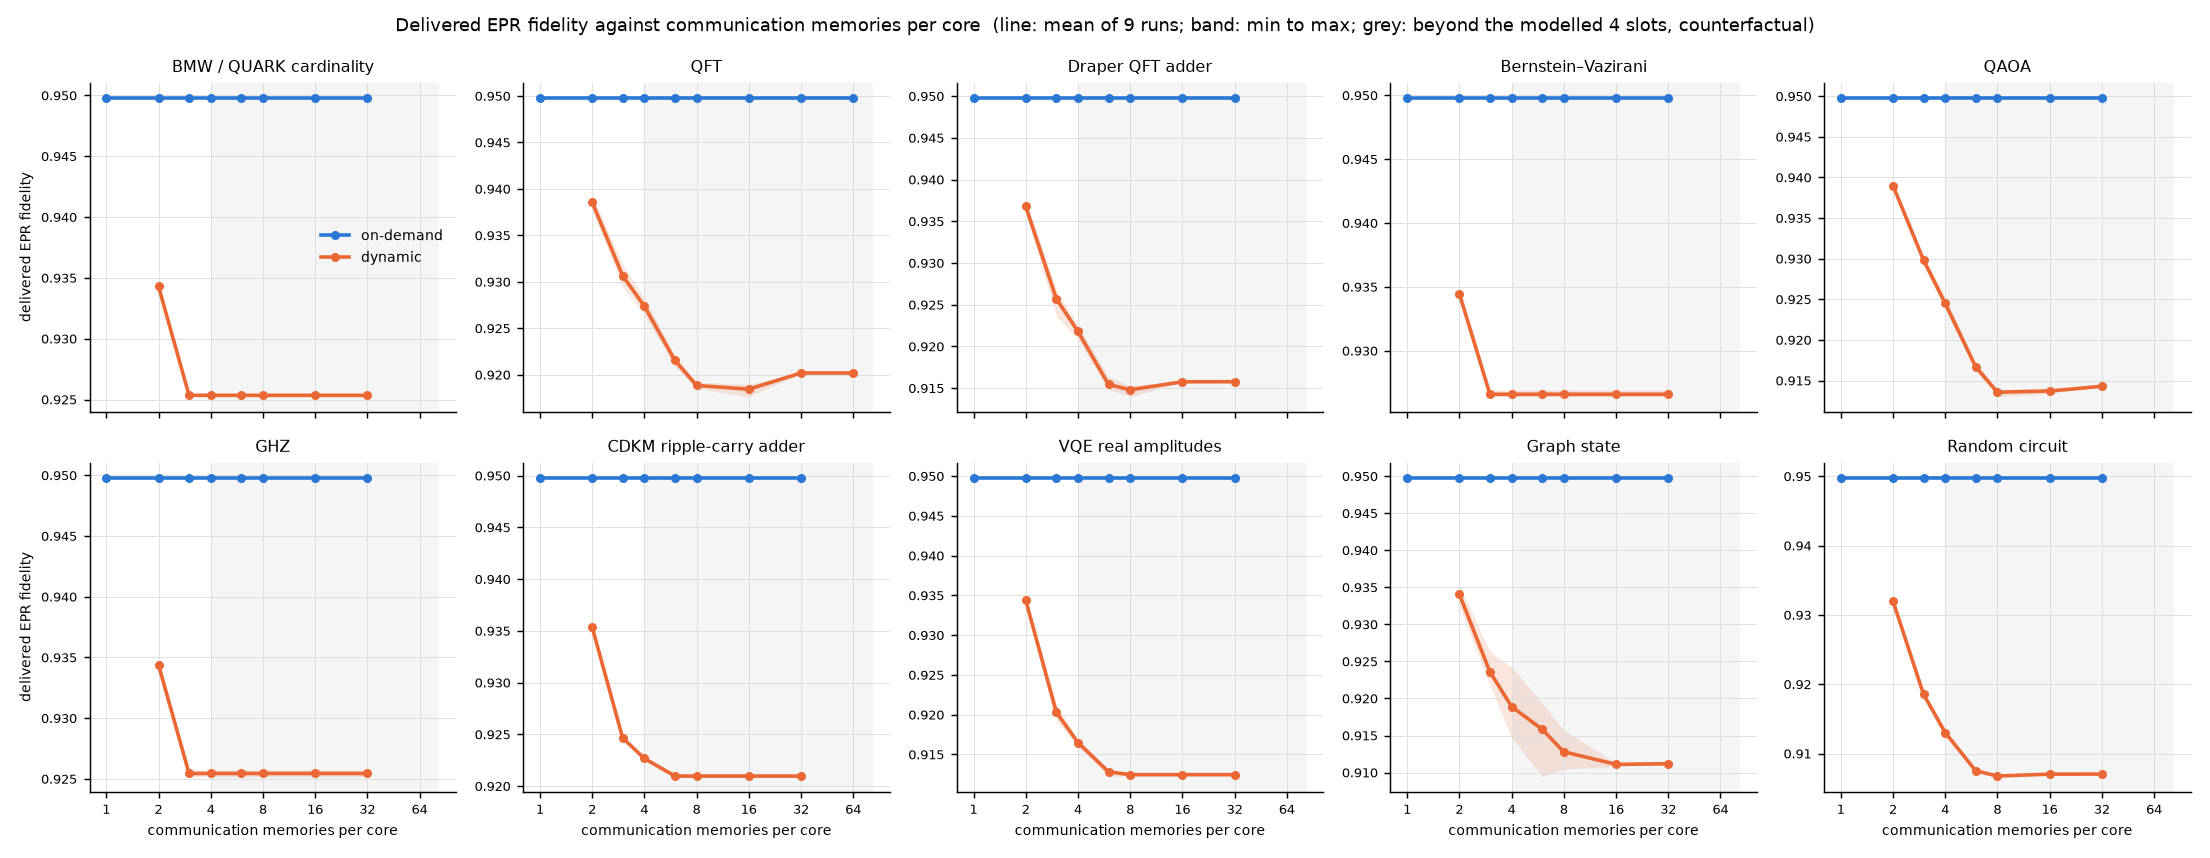
\includegraphics[width=\linewidth]{fidelity_vs_budget.png}
\caption{Delivered EPR fidelity against communication memories per core. Line: mean of nine runs; band: minimum to maximum; grey: counterfactual budgets.}
\label{fig:exp1-fidelity}
\end{figure}

\begin{table}[H]
\centering\small
\resizebox{\ifdim\width>\linewidth\linewidth\else\width\fi}{!}{%
\begin{tabular}{@{}lrrrrrrr@{}}
\toprule
Workload & 2 & 3 & 4 & 6$^*$ & 8$^*$ & 16$^*$ & 32$^*$ \\
\midrule
GHZ & 0.9344 & 0.9254 & 0.9254 & 0.9254 & 0.9254 & 0.9254 & 0.9254 \\
Bernstein--Vazirani & 0.9345 & 0.9266 & 0.9266 & 0.9266 & 0.9266 & 0.9266 & 0.9266 \\
BMW/QUARK cardinality & 0.9343 & 0.9253 & 0.9253 & 0.9253 & 0.9253 & 0.9253 & 0.9253 \\
VQE real amplitudes & 0.9344 & 0.9203 & 0.9165 & 0.9128 & 0.9125 & 0.9125 & 0.9125 \\
CDKM ripple-carry adder & 0.9354 & 0.9247 & 0.9227 & 0.9210 & 0.9210 & 0.9210 & 0.9210 \\
Graph state & 0.9341 & 0.9236 & 0.9189 & 0.9158 & 0.9128 & 0.9111 & 0.9112 \\
Draper QFT adder & 0.9368 & 0.9257 & 0.9218 & 0.9154 & 0.9148 & 0.9158 & 0.9158 \\
QAOA & 0.9390 & 0.9298 & 0.9245 & 0.9167 & 0.9136 & 0.9137 & 0.9143 \\
QFT & 0.9386 & 0.9306 & 0.9274 & 0.9215 & 0.9189 & 0.9185 & 0.9202 \\
Random circuit & 0.9320 & 0.9186 & 0.9130 & 0.9075 & 0.9068 & 0.9070 & 0.9071 \\
\bottomrule
\end{tabular}}
\caption{Delivered EPR fidelity, dynamic pre-generation. Budgets marked $^*$ are counterfactual (beyond the modelled four slots).}
\label{tab:exp1-fidelity-dynamic}
\end{table}

For the congested workloads dynamic is slower than on-demand at small budgets, because its prepared pairs may occupy up to $\text{budget}-1$ of the memories and requests then wait for a free one (Chapter~\ref{ch:why-dynamic}); the first budget at which
dynamic is faster than on-demand is 8 for graph state and Draper and 16 for QAOA and QFT. At 32 memories dynamic reaches $0.24$ to $0.30$\,ms against $1.11$ to $1.22$\,ms on-demand. Delivered fidelity under
dynamic is below the on-demand value ($0.9498$ in every cell) and falls as the compiler bank grows from two to about eight memories, by at most $0.043$ under ACE's one-second coherence time; the mechanism (pairs stored longer) is likely but was not measured.

\section{Sensitivity to the physical parameters}
This is exploratory, not a result of the study: the parameters are undecided. Five workloads, budgets $2,4,8,32$, mapping seed 42, were rerun with the group's multi-core paper's coherence time ($1$\,ms) and memory efficiency ($0.85$) in place of ACE's
($1$\,s and $0.95$). With the paper's values \textbf{every cached pair expires unused} (6 of 15\,700 compiler pairs were used), so dynamic pre-generation gives no benefit at all; on-demand fidelity falls from $0.9498$ to $0.7861$ in every workload and
budget, and on-demand latency rises by about $0.26$ to $0.42$\,ms. The congestion curves keep their shape. So the congestion results are structural and change little with these parameters, while the pre-generation and fidelity results depend entirely on them.

\section{Workload by workload}
Each paragraph is generated from the data: structural overload, the on-demand latency curve, the waiting at four memories, and the dynamic curve with the budget at which pre-generation first beats on-demand.
\subsection*{GHZ}
Structural overload at four slots: 0.0\% of active layers (one slot: 20\%). On-demand latency is 1.17\,ms with one memory, 1.17 with two, 1.17 with four and 1.17 with 32; it is within 5\% of the saturated value from 1 memory. At four memories 0.0\% of requests waited. Dynamic pre-generation takes 0.51\,ms with two memories, 0.26 with four and 0.26 with 32, and first beats on-demand at 2 memories; its delivered fidelity is 0.9344 at two memories and 0.9254 at 32 (on-demand: 0.9498).

\subsection*{Bernstein--Vazirani}
Structural overload at four slots: 0.0\% of active layers (one slot: 25\%). On-demand latency is 1.22\,ms with one memory, 1.22 with two, 1.22 with four and 1.22 with 32; it is within 5\% of the saturated value from 1 memory. At four memories 0.0\% of requests waited. Dynamic pre-generation takes 0.46\,ms with two memories, 0.24 with four and 0.24 with 32, and first beats on-demand at 2 memories; its delivered fidelity is 0.9345 at two memories and 0.9266 at 32 (on-demand: 0.9498).

\subsection*{BMW/QUARK cardinality}
Structural overload at four slots: 0.0\% of active layers (one slot: 20\%). On-demand latency is 1.12\,ms with one memory, 1.12 with two, 1.12 with four and 1.12 with 32; it is within 5\% of the saturated value from 1 memory. At four memories 0.0\% of requests waited. Dynamic pre-generation takes 0.49\,ms with two memories, 0.25 with four and 0.25 with 32, and first beats on-demand at 2 memories; its delivered fidelity is 0.9343 at two memories and 0.9253 at 32 (on-demand: 0.9498).

\subsection*{VQE real amplitudes}
Structural overload at four slots: 6.1\% of active layers (one slot: 55\%). On-demand latency is 2.32\,ms with one memory, 1.11 with two, 1.11 with four and 1.11 with 32; it is within 5\% of the saturated value from 2 memories. At four memories 0.0\% of requests waited. Dynamic pre-generation takes 1.52\,ms with two memories, 0.88 with four and 0.25 with 32, and first beats on-demand at 4 memories; its delivered fidelity is 0.9344 at two memories and 0.9125 at 32 (on-demand: 0.9498).

\subsection*{CDKM ripple-carry adder}
Structural overload at four slots: 0.6\% of active layers (one slot: 96\%). On-demand latency is 1.66\,ms with one memory, 1.24 with two, 1.14 with four and 1.14 with 32; it is within 5\% of the saturated value from 3 memories. At four memories 0.2\% of requests waited. Dynamic pre-generation takes 0.76\,ms with two memories, 0.30 with four and 0.30 with 32, and first beats on-demand at 2 memories; its delivered fidelity is 0.9354 at two memories and 0.9210 at 32 (on-demand: 0.9498).

\subsection*{Graph state}
Structural overload at four slots: 33.3\% of active layers (one slot: 100\%). On-demand latency is 9.14\,ms with one memory, 2.72 with two, 1.24 with four and 1.18 with 32; it is within 5\% of the saturated value from 6 memories. At four memories 2.9\% of requests waited. Dynamic pre-generation takes 6.36\,ms with two memories, 3.23 with four and 0.25 with 32, and first beats on-demand at 8 memories; its delivered fidelity is 0.9341 at two memories and 0.9112 at 32 (on-demand: 0.9498).

\subsection*{Draper QFT adder}
Structural overload at four slots: 41.3\% of active layers (one slot: 93\%). On-demand latency is 7.36\,ms with one memory, 2.16 with two, 1.15 with four and 1.13 with 32; it is within 5\% of the saturated value from 4 memories. At four memories 0.8\% of requests waited. Dynamic pre-generation takes 4.55\,ms with two memories, 2.48 with four and 0.25 with 32, and first beats on-demand at 8 memories; its delivered fidelity is 0.9368 at two memories and 0.9158 at 32 (on-demand: 0.9498).

\subsection*{QAOA}
Structural overload at four slots: 71.6\% of active layers (one slot: 98\%). On-demand latency is 10.92\,ms with one memory, 3.42 with two, 1.27 with four and 1.13 with 32; it is within 5\% of the saturated value from 6 memories. At four memories 5.8\% of requests waited. Dynamic pre-generation takes 6.89\,ms with two memories, 3.88 with four and 0.25 with 32, and first beats on-demand at 16 memories; its delivered fidelity is 0.9390 at two memories and 0.9143 at 32 (on-demand: 0.9498).

\subsection*{QFT}
Structural overload at four slots: 65.2\% of active layers (one slot: 95\%). On-demand latency is 14.42\,ms with one memory, 4.72 with two, 1.59 with four and 1.13 with 32; it is within 5\% of the saturated value from 8 memories. At four memories 13.0\% of requests waited. Dynamic pre-generation takes 10.06\,ms with two memories, 5.57 with four and 0.25 with 32, and first beats on-demand at 16 memories; its delivered fidelity is 0.9386 at two memories and 0.9202 at 32 (on-demand: 0.9498).

\subsection*{Random circuit}
Structural overload at four slots: 8.0\% of active layers (one slot: 90\%). On-demand latency is 2.99\,ms with one memory, 1.27 with two, 1.11 with four and 1.11 with 32; it is within 5\% of the saturated value from 3 memories. At four memories 0.1\% of requests waited. Dynamic pre-generation takes 1.91\,ms with two memories, 0.94 with four and 0.25 with 32, and first beats on-demand at 4 memories; its delivered fidelity is 0.9320 at two memories and 0.9071 at 32 (on-demand: 0.9498).


\chapter{The memory cut-off time}
\label{ch:cutoff}

A \emph{memory cut-off time} is a threshold after which a stored EPR pair is discarded and a new pair generated. Nothing new needs to be built to have one: ACE already has it, as the SeQUeNCe memory's
\code{cutoff_ratio}, and two other timers also end a stored pair's life.

\section{The timers}
\begin{description}
  \item[Memory cut-off.] When a pair is stored, an expiry is scheduled \code{cutoff_ratio} $\times$ coherence time later. At expiry the memory is reset (unless it is in an application) and returned to the free state; ACE then drops the
        pair from its cache and tells the compiler controller it expired. ACE's configuration never sets the ratio, so it is $1$ and the cut-off equals the coherence time, $1$\,s. A ratio written in the topology template was verified to reach every memory.
  \item[Reservation window.] A pair's booking ends with its window; an unused pair is released then. The window is $1000$\,ms for compiler pairs and, for the autonomous caches, runs to the next $0.2$\,s period boundary.
  \item[Planner lifetime.] The planner's \code{--coherence-time-layers} (10) says how far ahead a pair may be prepared; it is a planning assumption, tied to nothing physical.
\end{description}
Separately the stored state decoheres continuously at the rate $1/$coherence time, lowering fidelity but discarding nothing.

\section{What a discard does to compiler pairs}
\begin{table}[H]
\centering\small
\resizebox{\ifdim\width>\linewidth\linewidth\else\width\fi}{!}{%
\begin{tabular}{@{}llrrrrrrr@{}}
\toprule
Workload & Case & Done & Viol. & Consumed & Window & Cut-off & Bookings & Makespan ms \\
\midrule
ghz & ACE default: cut-off = coherence time (1 s), window 1000 ms & 24/24 & 0 & 48 & 0 & 0 & 48 & 303.5 \\
ghz & short reservation window only (20 ms) & 24/24 & 0 & 36 & 12 & 0 & 48 & 311.2 \\
ghz & cut-off ratio 0.02 (20 ms), window 1000 ms & 24/24 & 0 & 34 & 12 & 12 & 55 & 311.4 \\
ghz & cut-off ratio 0.005 (5 ms), window 1000 ms & 24/24 & 0 & 0 & 34 & 34 & 49 & 322.0 \\
ghz & cut-off ratio 0.02 and window 20 ms & 24/24 & 0 & 36 & 12 & 0 & 48 & 311.2 \\
graphstate & ACE default: cut-off = coherence time (1 s), window 1000 ms & 76/76 & 0 & 104 & 0 & 0 & 134 & 274.5 \\
graphstate & short reservation window only (20 ms) & 76/76 & 0 & 48 & 56 & 0 & 134 & 241.3 \\
graphstate & cut-off ratio 0.02 (20 ms), window 1000 ms & 76/76 & 0 & 24 & 32 & 32 & 179 & 351.8 \\
graphstate & cut-off ratio 0.005 (5 ms), window 1000 ms & 76/76 & 0 & 0 & 34 & 34 & 339 & 347.4 \\
graphstate & cut-off ratio 0.02 and window 20 ms & 76/76 & 0 & 48 & 56 & 0 & 134 & 242.5 \\
\bottomrule
\end{tabular}}
\caption{Which timer discards a cached pair (compiler pre-generation, 4 memories). Consumed: pairs used; Window: releases at the end of the reservation window; Cut-off: memory resets by the cut-off.}
\label{tab:cutoff-mechanism}
\end{table}

The earlier timer wins: with both at $20$\,ms the window fires first and no cut-off reset occurs. For compiler pairs a cut-off discards the pair and nothing replaces it: the controller only marks it expired, the request that wanted it
generates its own pair on demand, and all requests still complete. The run gets longer (graph state: $274.5$\,ms makespan by default, $351.8$\,ms with a $20$\,ms cut-off, $347.4$\,ms with $5$\,ms). In every case the number of window releases equals the number of cut-off resets,
consistent with a discarded pair's booking staying until its window ends (inferred from the counts).

\section{What a discard does to the autonomous caches}
\begin{table}[H]
\centering\small
\resizebox{\ifdim\width>\linewidth\linewidth\else\width\fi}{!}{%
\begin{tabular}{@{}llrrrrrr@{}}
\toprule
Strategy & Cut-off ratio & Generated & Used & Reported waste & Real unused & Latency ms & Fidelity \\
\midrule
continuous & 1 (default) & 44936 & 90 & 99.7\% & 99.80\% & 5.147 & 0.9297 \\
adaptive-continuous & 1 (default) & 5184 & 120 & 97.8\% & 97.69\% & 4.882 & 0.9258 \\
continuous & 0.2 & 44936 & 90 & 99.7\% & 99.80\% & 5.147 & 0.9297 \\
adaptive-continuous & 0.2 & 5184 & 120 & 97.8\% & 97.69\% & 4.882 & 0.9258 \\
continuous & 0.02 & 447388 & 122 & 10.0\% & 99.97\% & 4.865 & 0.9354 \\
adaptive-continuous & 0.02 & 41472 & 122 & 12.0\% & 99.71\% & 4.865 & 0.9354 \\
\bottomrule
\end{tabular}}
\caption{Autonomous caches on Random-16 (4 memories, coherence 1 s): effect of the memory cut-off. Reported waste omits cut-off discards.}
\label{tab:cutoff-cache}
\end{table}

A cut-off of $200$\,ms changes nothing, because the cache's window already ends at the next $0.2$\,s boundary. At $20$\,ms the cache discards and \emph{regenerates}: ten times more pairs are generated, the used pairs are fresher (fidelity $0.9297$ to $0.9354$) and latency
falls slightly ($5.15$ to $4.87$\,ms). ACE's waste counter does not see cut-off discards (it is incremented only when a generation rule expires at the window end), so the reported waste drops from $99.7\%$ to $10.0\%$ although $99.97\%$ of the generated pairs went unused;
waste measured with a cut-off must be computed as $1-\text{used}/\text{generated}$.

\section{Decisions}
Whether ``cut-off'' should mean discard-and-regenerate (the caches already do; compiler pre-generation falls back on demand and re-preparing would be a new feature); exposing the cut-off in milliseconds as a recorded study parameter; tying the planner's lifetime to it
and fixing the waste counter first; and the coherence time, which comes before any cut-off: with $1$\,s coherence a cut-off never acts, and with the group's $1$\,ms a cut-off equal to the coherence time would discard every cached pair before use.

\chapter{Can offline routing reduce the congestion?}
\label{ch:routing}

Experiment~2 (Chapter~\ref{ch:heatmap}) showed that at the modelled capacity of four memories nearly all overload is relay overload: it is caused by routes passing through the
central cores, not by routes starting or ending there. That raises a question about the routes. The mapper chooses, for every qubit move, one Dijkstra shortest path (fewest hops, link
reliability as the tie-break), without looking at what the other moves of the layer are doing. Many alternative shortest paths exist: between opposite corners of the $4\times4$ mesh there are
$\binom{6}{3}=20$. Could choosing them \emph{offline}, with the mapping untouched, spread the relay load and reduce the congestion?

\section{Method}
The mapping is held fixed: every qubit still moves from the same core to the same core in the same layer. Only the path of each move (a \emph{route}) is re-chosen, layer by layer
(layers are independent because a layer's routes start and end at fixed cores). For each layer that has any overload, the choice of one candidate path per route is made by solving a small
mixed-integer program exactly, minimising the \emph{excess}, the demand above capacity summed over cores. The candidates are all simple paths of at most the shortest length plus $0$ or $2$ hops,
and the mapper's own path is always a candidate, so the result is never worse than the baseline.

Two lower bounds hold for \emph{any} routing, so they show how much is left to gain. Endpoints do not depend on the path, so the demand of a core is at least its endpoint demand; and a route of shortest
length $k$ puts at least $2k$ hop touches ($k+1$ route touches) on the cores, so the total excess is at least the minimum total demand minus (cores $\times$ capacity). Both are tested.

Demand is counted two ways: by hops (the archive's counting) and by routes, the number of qubits in flight through a core, which is what the per-qubit scheduler experiences.

\section{Structural result}
\begin{table}[H]
\centering\small
\begin{tabular}{@{}rrrrrrr@{}}
\toprule
Capacity & Extra hops & Excess now & Excess after re-routing & Lower bound & Overloaded layers & Added hops \\
\midrule
1 & 0 & 27043 & 21894 (19.0\%) & 18336 & 4110 $\to$ 3801 & 0.00\% \\
1 & 2 & 27043 & 21018 (22.3\%) & 18336 & 4110 $\to$ 3621 & 2.55\% \\
2 & 0 & 10385 & 6771 (34.8\%) & 4995 & 1641 $\to$ 978 & 0.00\% \\
2 & 2 & 10385 & 6288 (39.5\%) & 4995 & 1641 $\to$ 840 & 1.48\% \\
3 & 0 & 4774 & 1791 (62.5\%) & 846 & 855 $\to$ 420 & 0.00\% \\
3 & 2 & 4774 & 1497 (68.6\%) & 846 & 855 $\to$ 327 & 0.98\% \\
4 & 0 & 2216 & 348 (84.3\%) & 78 & 482 $\to$ 102 & 0.00\% \\
4 & 2 & 2216 & 237 (89.3\%) & 78 & 482 $\to$ 48 & 0.36\% \\
\bottomrule
\end{tabular}
\caption{Offline re-routing, mesh, route counting, pooled over ten benchmarks and three mapping seeds. Excess is demand above capacity.}
\label{tab:routing-mesh}
\end{table}

Pooled over the ten benchmarks, the best routing removes most of the excess at the modelled capacity: with route counting at capacity four, shortest paths alone cut the excess from 2\,216 to 348 (an 84.3\% reduction)
and the layers with any overload from 482 to 102; allowing two extra hops cuts it to 237 (89.3\%) at a cost of 0.36\% more hops. The gain shrinks as the capacity shrinks (19.0\% at capacity one),
because there the total relay volume, not the choice of path, is the limit, which the volume bound shows. With hop counting the reductions are smaller (65.6\% at capacity four).

\section{Simulated effect}
The structural gain would be an artefact if it did not survive the simulator, so the re-routed traces were run in ACE next to the original routes, on-demand, at the budget they were optimised for, with the same
mapping, endpoints, physics seeds and parameters. Three mapping seeds and three physics seeds give nine paired runs per cell.
\begin{table}[H]
\centering\small
\resizebox{\ifdim\width>\linewidth\linewidth\else\width\fi}{!}{%
\begin{tabular}{@{}lrrrrr@{}}
\toprule
Workload & Mem. & Original & Re-routed & +2 hops & Waited \\
\midrule
Graph state & 2 & 2.72 & 1.53 (+42.3\% $\pm$9.9; 9/9) & 1.41 (+46.6\% $\pm$8.9; 9/9) & 0.281 $\to$ 0.086 \\
Graph state & 3 & 1.53 & 1.15 (+22.9\% $\pm$11.8; 9/9) & 1.19 (+19.6\% $\pm$13.5; 9/9) & 0.121 $\to$ 0.000 \\
Graph state & 4 & 1.24 & 1.16 (+6.0\% $\pm$7.6; 7/9) & 1.21 (+1.9\% $\pm$8.9; 4/9) & 0.029 $\to$ 0.000 \\
Draper QFT adder & 2 & 2.16 & 1.69 (+21.1\% $\pm$7.9; 9/9) & 1.48 (+31.1\% $\pm$6.8; 9/9) & 0.211 $\to$ 0.115 \\
Draper QFT adder & 3 & 1.30 & 1.16 (+10.3\% $\pm$3.3; 9/9) & 1.16 (+10.5\% $\pm$3.7; 9/9) & 0.055 $\to$ 0.007 \\
Draper QFT adder & 4 & 1.15 & 1.13 (+1.3\% $\pm$1.3; 8/9) & 1.14 (+1.1\% $\pm$0.8; 9/9) & 0.008 $\to$ 0.000 \\
QAOA & 2 & 3.42 & 2.24 (+34.5\% $\pm$2.4; 9/9) & 2.12 (+38.0\% $\pm$2.4; 9/9) & 0.376 $\to$ 0.206 \\
QAOA & 3 & 1.74 & 1.25 (+28.4\% $\pm$2.3; 9/9) & 1.19 (+31.4\% $\pm$2.2; 9/9) & 0.172 $\to$ 0.037 \\
QAOA & 4 & 1.27 & 1.13 (+10.9\% $\pm$1.7; 9/9) & 1.13 (+11.5\% $\pm$1.6; 9/9) & 0.058 $\to$ 0.003 \\
QFT & 2 & 4.72 & 3.49 (+26.1\% $\pm$2.4; 9/9) & 3.03 (+35.9\% $\pm$2.1; 9/9) & 0.430 $\to$ 0.312 \\
QFT & 3 & 2.39 & 1.53 (+35.9\% $\pm$2.2; 9/9) & 1.47 (+38.2\% $\pm$2.3; 9/9) & 0.249 $\to$ 0.097 \\
QFT & 4 & 1.59 & 1.19 (+25.2\% $\pm$2.4; 9/9) & 1.17 (+26.6\% $\pm$2.0; 9/9) & 0.130 $\to$ 0.018 \\
Random circuit & 2 & 1.27 & 1.13 (+10.6\% $\pm$1.3; 9/9) & 1.12 (+11.7\% $\pm$1.3; 9/9) & 0.042 $\to$ 0.007 \\
Random circuit & 3 & 1.12 & 1.11 (+1.2\% $\pm$0.3; 9/9) & 1.11 (+1.3\% $\pm$0.3; 9/9) & 0.006 $\to$ 0.000 \\
Random circuit & 4 & 1.11 & 1.11 (+0.2\% $\pm$0.1; 9/9) & 1.11 (+0.2\% $\pm$0.2; 8/9) & 0.001 $\to$ 0.000 \\
\bottomrule
\end{tabular}}
\caption{Simulated on-demand latency (ms), mesh: original routes against offline re-routing. Brackets: paired reduction in latency (positive = faster), sd, pairs faster of nine.}
\label{tab:routing-sim-mesh}
\end{table}

Re-routing alone makes on-demand requests faster in nearly every pair. At two memories the latency falls by 21\% to 42\% on the four congested workloads (graph state, Draper, QAOA, QFT) and by 11\% on the random circuit; at the modelled four memories by 25\% for QFT, 11\% for QAOA and 6\% for graph state,
and by 1\% or less where there was little congestion. The fraction of requests that had to wait falls accordingly. Two extra hops help at two memories (QFT 26\% to 36\%) and change little at four (within about 1.5 percentage points, except graph state, where they cost 4 points): the added hops cost about as much as the avoided waiting saves.

\section{The torus}
On the torus, which has more paths between cores, the optimum is closer to the lower bound still: at capacity four the excess falls from 493 to 15 (97.0\%), against a lower bound of 6, and with two extra hops it reaches the bound.
\begin{table}[H]
\centering\small
\begin{tabular}{@{}rrrrrrr@{}}
\toprule
Capacity & Extra hops & Excess now & Excess after re-routing & Lower bound & Overloaded layers & Added hops \\
\midrule
1 & 0 & 20202 & 15858 (21.5\%) & 14847 & 3826 $\to$ 3339 & 0.00\% \\
1 & 2 & 20202 & 15387 (23.8\%) & 14847 & 3826 $\to$ 3312 & 1.73\% \\
2 & 0 & 6108 & 3351 (45.1\%) & 2847 & 1319 $\to$ 702 & 0.00\% \\
2 & 2 & 6108 & 3108 (49.1\%) & 2847 & 1319 $\to$ 630 & 0.93\% \\
3 & 0 & 1852 & 363 (80.4\%) & 303 & 562 $\to$ 162 & 0.00\% \\
3 & 2 & 1852 & 342 (81.5\%) & 303 & 562 $\to$ 159 & 0.09\% \\
4 & 0 & 493 & 15 (97.0\%) & 6 & 220 $\to$ 15 & 0.00\% \\
4 & 2 & 493 & 6 (98.8\%) & 6 & 220 $\to$ 6 & 0.04\% \\
\bottomrule
\end{tabular}
\caption{Offline re-routing, torus, route counting, pooled over ten benchmarks and three mapping seeds. Excess is demand above capacity.}
\label{tab:routing-torus}
\end{table}

Simulated on the torus, re-routing makes requests faster at two memories (latency falls by 15\% for QFT, 32\% for QAOA, 36\% for Draper) but little at the modelled four (by 6.8\% for QFT, 3.2\% for QAOA, about 2\% or nothing for the others), because the torus is already close to its latency floor there.
\begin{table}[H]
\centering\small
\resizebox{\ifdim\width>\linewidth\linewidth\else\width\fi}{!}{%
\begin{tabular}{@{}lrrrrr@{}}
\toprule
Workload & Mem. & Original & Re-routed & +2 hops & Waited \\
\midrule
Graph state & 2 & 1.86 & 1.27 (+31.2\% $\pm$7.2; 9/9) & 1.28 (+31.0\% $\pm$6.9; 9/9) & 0.157 $\to$ 0.033 \\
Graph state & 3 & 1.25 & 1.10 (+11.0\% $\pm$7.4; 8/9) & 1.12 (+10.3\% $\pm$8.7; 8/9) & 0.033 $\to$ 0.000 \\
Graph state & 4 & 1.11 & 1.12 (-0.4\% $\pm$1.7; 1/9) & 1.11 (+0.3\% $\pm$3.9; 2/9) & 0.000 $\to$ 0.000 \\
Draper QFT adder & 2 & 2.25 & 1.45 (+35.6\% $\pm$1.9; 9/9) & 1.26 (+44.0\% $\pm$1.4; 9/9) & 0.226 $\to$ 0.075 \\
Draper QFT adder & 3 & 1.28 & 1.15 (+10.5\% $\pm$1.8; 9/9) & 1.14 (+10.7\% $\pm$1.0; 9/9) & 0.053 $\to$ 0.007 \\
Draper QFT adder & 4 & 1.13 & 1.11 (+1.8\% $\pm$0.6; 9/9) & 1.11 (+1.6\% $\pm$0.8; 9/9) & 0.008 $\to$ 0.000 \\
QAOA & 2 & 2.47 & 1.66 (+32.3\% $\pm$4.7; 9/9) & 1.62 (+34.2\% $\pm$4.7; 9/9) & 0.265 $\to$ 0.111 \\
QAOA & 3 & 1.40 & 1.15 (+17.6\% $\pm$4.6; 9/9) & 1.14 (+18.3\% $\pm$4.3; 9/9) & 0.083 $\to$ 0.004 \\
QAOA & 4 & 1.17 & 1.13 (+3.2\% $\pm$2.8; 9/9) & 1.13 (+3.1\% $\pm$2.6; 9/9) & 0.016 $\to$ 0.000 \\
QFT & 2 & 2.79 & 2.37 (+14.7\% $\pm$7.3; 9/9) & 2.42 (+12.7\% $\pm$7.8; 9/9) & 0.303 $\to$ 0.221 \\
QFT & 3 & 1.51 & 1.21 (+19.3\% $\pm$6.0; 9/9) & 1.24 (+17.3\% $\pm$6.1; 9/9) & 0.102 $\to$ 0.023 \\
QFT & 4 & 1.21 & 1.13 (+6.8\% $\pm$3.2; 9/9) & 1.12 (+7.3\% $\pm$3.0; 9/9) & 0.028 $\to$ 0.001 \\
Random circuit & 2 & 1.19 & 1.11 (+6.1\% $\pm$0.9; 9/9) & 1.11 (+6.3\% $\pm$0.9; 9/9) & 0.022 $\to$ 0.002 \\
Random circuit & 3 & 1.11 & 1.11 (+0.4\% $\pm$0.1; 9/9) & 1.11 (+0.3\% $\pm$0.1; 9/9) & 0.001 $\to$ 0.000 \\
Random circuit & 4 & 1.11 & 1.11 (-0.0\% $\pm$0.1; 1/9) & 1.11 (+0.0\% $\pm$0.1; 3/9) & 0.000 $\to$ 0.000 \\
\bottomrule
\end{tabular}}
\caption{Simulated on-demand latency (ms), torus: original routes against offline re-routing. Brackets: paired reduction, sd, pairs faster of nine.}
\label{tab:routing-sim-torus}
\end{table}


\section{What can and cannot be concluded}
Offline routing \emph{can} reduce congestion: with the mapping fixed, an exact offline choice of paths removes most of the excess demand at the modelled capacity and the simulated latencies fall with it. These
are results for an offline optimum with global knowledge of every layer, computed per layer for the capacity the hardware has; a practical routing algorithm would be a heuristic for the same problem and would be bounded by it.
Not shown here: the effect on pre-generation policies (only on-demand was simulated), joint optimisation of mapping and routing, fidelity effects (the on-demand fidelity does not depend on waiting), and a routing policy that does not know
the layer in advance. Whether to pursue the research further is therefore a question about those directions, and the bounds above say how much headroom each could have.

\chapter{The torus topology}
\label{ch:torus}

\section{What changes}
A $4\times4$ torus joins the opposite edges of the mesh with eight extra links, so every core has four neighbours and the longest path shrinks from six hops to four. Everything else is held as in the
mesh experiments: the same ten benchmarks, the same mapper (HQA) with the same seeds, the same ACE parameters, the same link length for every link (a folded layout; the wrap links are not longer),
the same scheduler, budgets, policies, physics seeds and controls.

\paragraph{Routing.} The routes are the mapper's own: a Dijkstra search for the path with the fewest hops, with the product of link reliabilities as the tie-break (route model \code{shortest}), exactly as for the mesh
traces. The mapping-only path of the study script was checked to reproduce the archived mesh trace line for line before it was used for the torus. ACE itself needed three changes: trace validation
knows wrap-around links; the topology file is generated from the mesh file by adding the eight wrap links in the mesh's own link format (every router then has four quantum links, tested by loading it in ACE);
and a torus trace is refused on a mesh topology file and the reverse.

\paragraph{One caveat.} The mapper is run on the torus graph, so the torus traces differ from the mesh traces in the placement as well as the routes. Differences below are differences of the two systems, not of the topology alone.

\section{Results}
Torus traces need 11\% to 37\% fewer hops than the mesh traces (CDKM 11\%, QFT 23\%, QAOA 16\%, GHZ 25\%, VQE 37\%). Every control passed on all 1\,368 runs, as for the mesh (Chapter~\ref{ch:exp1}).
\begin{table}[H]
\centering\small
\begin{tabular}{@{}lrrrrr@{}}
\toprule
Workload & Hops & Overload\% at C=4 & On-demand ms, 2 mem. & On-demand ms, 4 mem. & Dynamic ms, 8 mem. \\
\midrule
GHZ & 24/18 & 0.0/0.0 & 1.17/1.15 & 1.17/1.15 & 0.26/0.28 \\
Bernstein--Vazirani & 25/21 & 0.0/0.0 & 1.22/1.11 & 1.22/1.11 & 0.24/0.23 \\
BMW/QUARK cardinality & 144/108 & 0.0/0.0 & 1.12/1.10 & 1.12/1.10 & 0.25/0.25 \\
VQE real amplitudes & 104/66 & 6.1/1.5 & 1.11/1.14 & 1.11/1.14 & 0.25/0.30 \\
CDKM ripple-carry adder & 456/406 & 0.6/0.6 & 1.24/1.11 & 1.14/1.09 & 0.30/0.29 \\
Graph state & 76/60 & 33.3/38.9 & 2.72/1.86 & 1.24/1.11 & 0.95/0.62 \\
Draper QFT adder & 1310/984 & 41.3/25.8 & 2.16/2.25 & 1.15/1.13 & 0.89/0.74 \\
QAOA & 3068/2562 & 71.6/57.9 & 3.42/2.47 & 1.27/1.17 & 1.86/1.10 \\
QFT & 2510/1938 & 65.2/58.0 & 4.72/2.79 & 1.59/1.21 & 2.78/1.16 \\
Random circuit & 11688/9574 & 8.0/3.4 & 1.27/1.19 & 1.11/1.11 & 0.38/0.29 \\
\bottomrule
\end{tabular}
\caption{Mesh/torus. Hops: mean requests per trace. Overload: \% of active layers with any core above capacity 4. Latencies are means over nine runs.}
\label{tab:torus}
\end{table}

On-demand latency under congestion improves: at two memories QFT goes from $4.72$ to $2.79$\,ms, QAOA from $3.42$ to $2.47$\,ms and graph state from $2.72$ to $1.86$\,ms; at four memories QFT from $1.59$ to $1.21$\,ms. Dynamic pre-generation also gets faster under congestion (QFT at eight memories: $2.78$ to $1.16$\,ms). The structural overload at capacity four falls for most workloads (QFT 65.2\% to 58.0\%, QAOA 71.6\% to 57.9\%, Draper 41.3\% to 25.8\%) but not for graph state, where
it rises from 33.3\% to 38.9\% (only six layers are active, so a single layer is 17 percentage points). Draper at two memories is slightly slower on the torus ($2.16$ to $2.25$\,ms).

\clearpage\newgeometry{margin=12mm}\begin{landscape}
\begin{figure}[p]
\centering
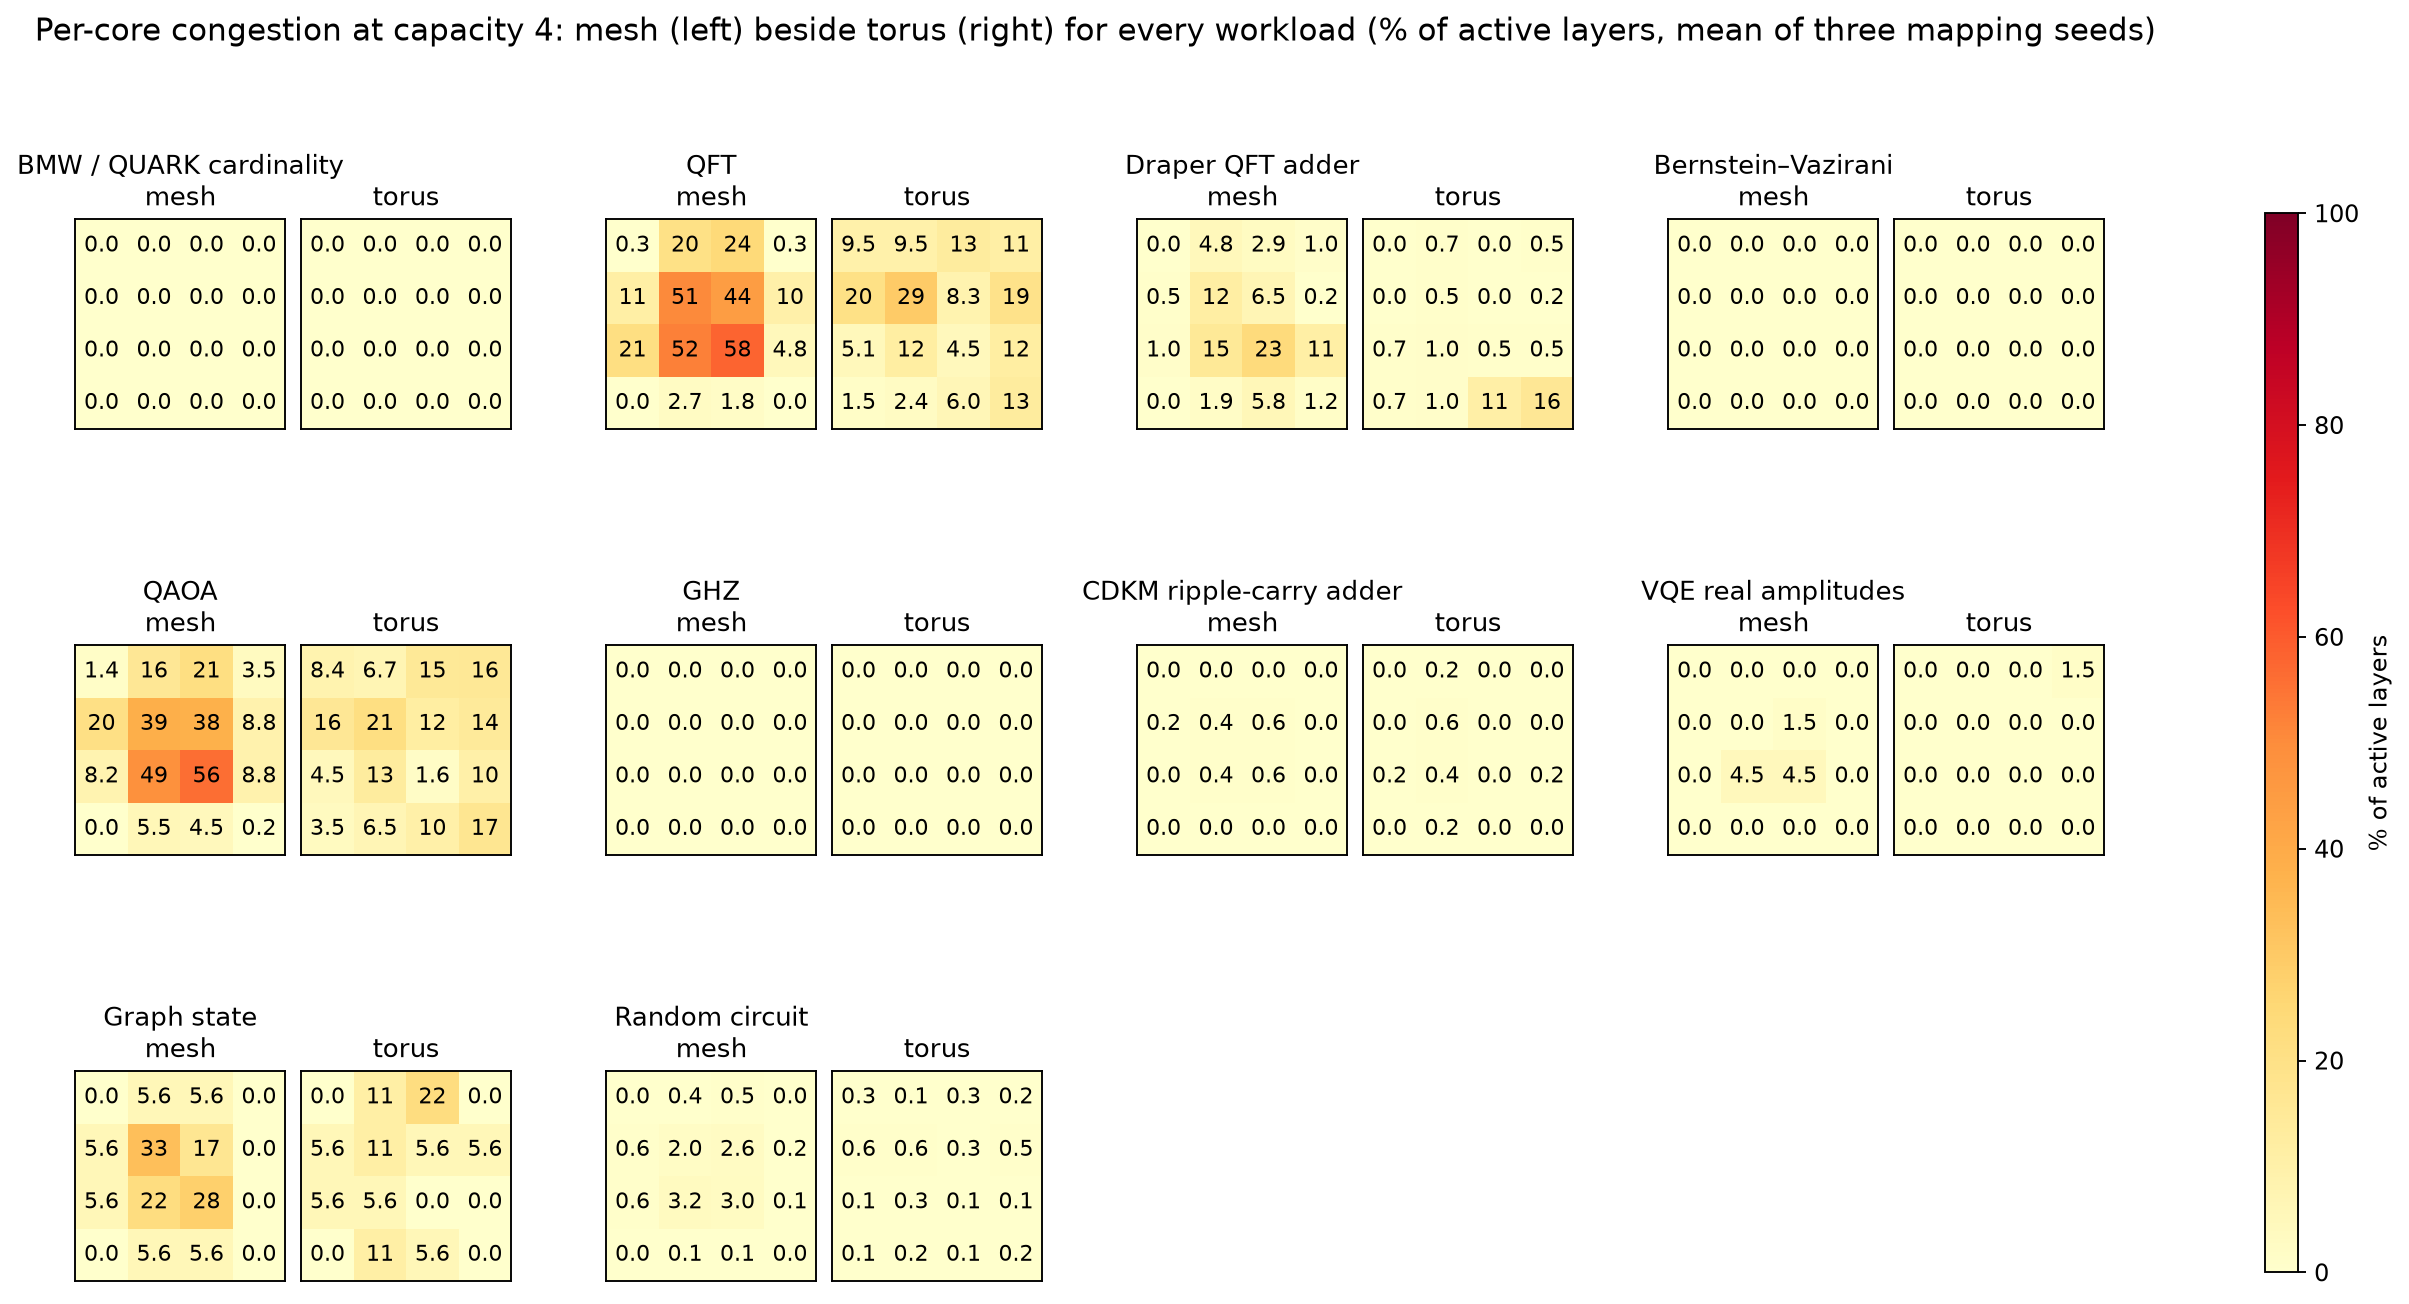
\includegraphics[width=\linewidth,height=0.82\textheight,keepaspectratio]{mesh_vs_torus_heatmaps.png}
\caption{Per-core congestion at capacity 4 on the mesh (left of each pair) and on the torus (right), for every workload. The torus lowers the overload in five workloads, leaves four unchanged and raises it for graph state; the traces differ in placement as well as topology.}
\label{fig:mesh-vs-torus}
\end{figure}
\end{landscape}\clearpage\restoregeometry


\chapter{Run times}
\label{ch:runtimes}

Wall-clock times on the development machine (8 CPUs). An \emph{invocation} is one process running one benchmark at one budget and policy for three physics seeds.
Times from parallel runs include contention from the other jobs; the serial pass was run one invocation at a time and is the cleanest per-benchmark measurement. It was not isolated from light unrelated work on the machine (file edits, short tests), so expect a few percent of noise.
\begin{table}[H]
\centering\small
\begin{tabular}{@{}lrrr@{}}
\toprule
Experiment & Jobs & Runs & Wall clock \\
\midrule
Experiment 1, mesh & 4 & 1368 & 24.5 min \\
Experiment 1, torus & 4 & 1368 & 25.2 min \\
Sensitivity arm & 4 & 120 & 105.0 s \\
Serial timing pass & 1 & 270 & 8.6 min \\
\bottomrule
\end{tabular}
\caption{Wall-clock time of each experiment.}
\label{tab:runtimes-total}
\end{table}

\begin{table}[H]
\centering\small
\resizebox{\ifdim\width>\linewidth\linewidth\else\width\fi}{!}{%
\begin{tabular}{@{}lrrrrrrrrr@{}}
\toprule
Benchmark & \multicolumn{5}{c}{on-demand, memories} & \multicolumn{4}{c}{dynamic, memories} \\
 & 1 & 2 & 4 & 8 & 32 & 2 & 4 & 8 & 32 \\
\midrule
GHZ & 0.4 & 0.4 & 0.4 & 0.4 & 0.4 & 0.4 & 0.4 & 0.4 & 0.4 \\
Bernstein-Vazirani & 0.4 & 0.4 & 0.4 & 0.4 & 0.4 & 0.4 & 0.4 & 0.4 & 0.4 \\
BMW/QUARK cardinality & 0.5 & 0.5 & 0.5 & 0.5 & 0.5 & 0.5 & 0.5 & 0.5 & 0.5 \\
VQE real amplitudes & 0.4 & 0.4 & 0.4 & 0.4 & 0.4 & 0.4 & 0.5 & 0.5 & 0.5 \\
CDKM ripple-carry adder & 0.6 & 0.6 & 0.6 & 0.6 & 0.6 & 0.7 & 0.7 & 0.7 & 0.8 \\
Graph state & 0.4 & 0.4 & 0.4 & 0.4 & 0.4 & 0.4 & 0.4 & 0.4 & 0.4 \\
Draper QFT adder & 1.1 & 1.1 & 1.1 & 1.1 & 1.2 & 1.2 & 1.4 & 1.4 & 1.6 \\
QAOA & 2.1 & 2.1 & 2.1 & 2.2 & 2.4 & 2.4 & 2.8 & 3.1 & 3.5 \\
QFT & 1.8 & 1.8 & 1.7 & 1.8 & 2.0 & 1.9 & 2.2 & 2.5 & 2.9 \\
Random circuit & 7.8 & 7.9 & 8.0 & 8.0 & 8.8 & 10.6 & 14.1 & 14.9 & 15.3 \\
\bottomrule
\end{tabular}}
\caption{Seconds of real time per simulation run, one run at a time (serial pass, mapping seed 42; mean over three physics seeds).}
\label{tab:runtimes-serial}
\end{table}

The CGP and ACGP runs of Chapter~\ref{ch:four-policies} (four parallel jobs next to other work on the machine) finished their first $380$ of $426$ mesh invocations in $126$\,minutes; the rest are the random circuit's large-memory runs, which each take from $10$\,min to over an hour and were set aside; the driver was stopped before it wrote its timing file, so the per-invocation times of those runs were not recorded. The $70$ diagnostic runs (Chapter~\ref{ch:why-dynamic}), run two at a time, took $47$\,minutes; their individual times are in each JSON file (\code{wall_seconds}). The heatmap regeneration takes 2.7\,s and the endpoint-versus-relay split 4.3\,s. The new scheduler costs a few percent more real time than the legacy one on the larger traces, because it reads the
reservation tables at admission. Real time is unrelated to the simulated latencies the experiments report. The full set of numbers, including parallel per-benchmark sums, is in \code{docs/reports/run-times.md}.

\chapter{Why dynamic pre-generation can be slower than on-demand}
\label{ch:why-dynamic}

The aim of compiler-driven pre-generation is a latency comparable to or better than on-demand generation (ODG) with fewer wasted pairs than the autonomous
protocols (CGP, ACGP). Experiment~1 found that, on the corrected scheduler and at the modelled memory counts, dynamic pre-generation is \emph{slower} than ODG on the congested benchmarks
(QFT at four memories: ODG $1.59$\,ms, dynamic $5.57$\,ms, mean of nine runs), and faster once memory is plentiful (QFT at sixteen memories: $1.14$ against $0.80$\,ms). The tables of this chapter use one mapping seed (42) unless they say otherwise, so their QFT numbers ($1.57$ and $5.46$\,ms at four memories) differ slightly. This chapter finds out why.
Everything here was measured on ACE with the corrected scheduler, and the explanation is checked against the code (Section~\ref{sec:code-reading}).

\section{What the old, serialized scheduler showed}
The scheduler used before the corrections let each core serve one request per batch. Under it the same comparison gave the opposite sign
(Table~\ref{tab:legacy-vs-corrected}): dynamic was faster than ODG at every memory count, by $41\%$ on QFT at four memories in the old scheduler's own latency.
Two things changed. First, the old latency started a request's clock when its batch was submitted, so the long waits for earlier batches were not in it; counting them
(``old common'') the gain on QFT at four memories is $11\%$, and the whole trace took $13.2$\,s with ODG and $12.3$\,s with dynamic (Table~\ref{tab:legacy-makespan}).
Second, the old scheduler let a core serve one request at a time, and in the old QFT runs at four memories no request waited for a memory under either policy
(retry wait $0.0$\,ms for ODG and for dynamic), while ODG's own latency did not respond to the number of memories at all. The corrected scheduler runs the requests of a layer
concurrently, as the hardware would, and the waiting appears.
\begin{table}[H]
\centering\small
\resizebox{\ifdim\width>\linewidth\linewidth\else\width\fi}{!}{%
\begin{tabular}{@{}llrrrrrrrrr@{}}
\toprule
Workload & Mem. & Old own ODG & Old own Dyn. & Old own gain & Old common ODG & Old common Dyn. & Old common gain & New common ODG & New common Dyn. & New common gain \\
\midrule
QFT & 2 & 1.11 & 0.93 & 17\% & 25.06 & 23.95 & 4\% & 4.72 & 10.06 & -113\% \\
QFT & 3 & 1.11 & 0.77 & 31\% & 25.06 & 23.03 & 8\% & 2.39 & 7.49 & -214\% \\
QFT & 4 & 1.11 & 0.65 & 41\% & 25.06 & 22.30 & 11\% & 1.59 & 5.57 & -250\% \\
QFT & 32 & 1.11 & 0.25 & 77\% & 25.06 & 20.28 & 19\% & 1.13 & 0.25 & 78\% \\
QAOA & 2 & 1.11 & 0.91 & 18\% & 13.39 & 12.56 & 6\% & 3.42 & 6.89 & -101\% \\
QAOA & 3 & 1.11 & 0.74 & 34\% & 13.39 & 11.84 & 12\% & 1.74 & 5.33 & -207\% \\
QAOA & 4 & 1.11 & 0.61 & 45\% & 13.39 & 11.34 & 15\% & 1.27 & 3.88 & -205\% \\
QAOA & 32 & 1.11 & 0.25 & 78\% & 13.39 & 10.14 & 24\% & 1.13 & 0.25 & 78\% \\
Draper QFT adder & 2 & 1.12 & 0.84 & 26\% & 9.40 & 8.57 & 9\% & 2.16 & 4.55 & -111\% \\
Draper QFT adder & 3 & 1.12 & 0.60 & 47\% & 9.40 & 7.91 & 16\% & 1.30 & 3.67 & -182\% \\
Draper QFT adder & 4 & 1.12 & 0.47 & 58\% & 9.40 & 7.55 & 20\% & 1.15 & 2.48 & -116\% \\
Draper QFT adder & 32 & 1.12 & 0.25 & 78\% & 9.40 & 7.05 & 25\% & 1.13 & 0.25 & 78\% \\
Graph state & 2 & 1.16 & 0.84 & 27\% & 9.98 & 9.05 & 9\% & 2.72 & 6.36 & -134\% \\
Graph state & 3 & 1.16 & 0.63 & 46\% & 9.98 & 8.42 & 16\% & 1.53 & 5.01 & -228\% \\
Graph state & 4 & 1.16 & 0.49 & 58\% & 9.98 & 7.91 & 21\% & 1.24 & 3.23 & -161\% \\
Graph state & 32 & 1.16 & 0.25 & 78\% & 9.98 & 7.28 & 27\% & 1.18 & 0.25 & 79\% \\
GHZ & 2 & 1.17 & 0.51 & 56\% & 1.17 & 0.51 & 56\% & 1.17 & 0.51 & 56\% \\
GHZ & 3 & 1.17 & 0.26 & 78\% & 1.17 & 0.26 & 78\% & 1.17 & 0.26 & 78\% \\
GHZ & 4 & 1.17 & 0.26 & 78\% & 1.17 & 0.26 & 78\% & 1.17 & 0.26 & 78\% \\
GHZ & 32 & 1.17 & 0.26 & 78\% & 1.17 & 0.26 & 78\% & 1.17 & 0.26 & 78\% \\
\bottomrule
\end{tabular}}
\caption{Request latency (ms) of on-demand (ODG) and dynamic (Dyn.) and the dynamic gain $(\text{ODG}-\text{Dyn.})/\text{ODG}$. Old own: the old serialized scheduler's own latency, whose clock for a request starts when its batch is submitted. Old common: the same old runs under the common definition, which also counts the wait for earlier batches. New common: the corrected per-qubit scheduler under the common definition. Mean of nine runs (three mapping seeds, three physics seeds).}
\label{tab:legacy-vs-corrected}
\end{table}

\begin{table}[H]
\centering\small
\resizebox{\ifdim\width>\linewidth\linewidth\else\width\fi}{!}{%
\begin{tabular}{@{}lrrrr@{}}
\toprule
Workload & Old ODG & Old Dyn. & New ODG & New Dyn. \\
\midrule
QFT & 13.23 & 12.34 & 4.66 & 5.75 \\
QAOA & 12.76 & 11.72 & 5.48 & 6.62 \\
Draper QFT adder & 7.64 & 6.97 & 4.88 & 5.03 \\
Graph state & 0.40 & 0.36 & 0.24 & 0.26 \\
GHZ & 0.33 & 0.30 & 0.33 & 0.30 \\
\bottomrule
\end{tabular}}
\caption{End-to-end time of the whole trace (s) at four memories per core, old serialized scheduler and corrected scheduler (mean of nine runs).}
\label{tab:legacy-makespan}
\end{table}


\section{What the code does with a pre-generated pair}
\label{sec:code-reading}
The explanation below was checked against the source, not inferred from the results. File and line numbers refer to the repository at the commit that contains this report.

\begin{enumerate}
  \item \textbf{When a dynamic preparation starts.} The planner gives each request a generation layer. For the dynamic policy the candidate layers are tried from the one just
    before the request's own layer, backwards (\code{compiler_trace.py:254}), and the first one with room is taken. The controller launches a layer's preparations when that layer is
    activated (\code{request_scheduler.py:151--158}, \code{compiler_scheduler.py:66}). So a pair for a request in layer $L$ is normally started at the \emph{start} of layer $L-1$
    and has to wait for all of layer $L-1$ to finish before its request can even be released. The lookahead of eight layers is only an upper limit; varying it made no difference
    (Section~\ref{sec:ablations}).
  \item \textbf{What a prepared pair occupies.} A preparation books one memory card at each of its two cores, with a window of 1\,000\,ms
    (\code{adaptive_continuous.py:192--236}), and it may not exceed the compiler cap, the same counter that limits the autonomous protocol
    (\code{adaptive_continuous.py:201}). The booking is released only when the pair is consumed (\code{reservation.py:473}) or its window ends.
    If the cap is reached the preparation is rejected and retried every millisecond until its request starts (\code{compiler_scheduler.py:113--120}).
  \item \textbf{A request that has a ready pair still needs a memory of its own.} Admission asks for a free card at both cores, and a card with any overlapping booking
    is not free (\code{request_scheduler.py:202--215, 232--255}); the prepared pair's own booking overlaps. When the request's reservation runs, the generation protocol
    looks for a ready pair for the same two cores, and if it finds one it \emph{swaps} the pair's state into the request's own memory after a classical delay
    (\code{generation.py:265--296, 301--343}) and only then releases the prepared pair's memory (\code{generation.py:342}). So for a short time a hit holds \emph{two} cards
    at each core. This is a property of ACE's design, not of the compiler policy, and it is why requests served from a ready pair can still wait for admission.
  \item \textbf{What an on-demand request occupies.} One card per core, from admission until completion. Its booking window is the request duration (50\,ms), but the booking is
    released at completion, so what matters is the time it exists, about 6\,ms in the measurements, not the window.
  \item \textbf{CGP and ACGP.} Every cycle of the autonomous protocol draws a neighbour by roulette wheel over a probability table (\code{adaptive_continuous.py:262--276}) and books one card at both
    ends until a 0.2\,s boundary within the next 0.2\,s (\code{adaptive_continuous.py:147--178}; the period is $2\times10^{11}$\,ps, \code{node.py:57}), as long as fewer than the cap are in use.
    The table is uniform for CGP (\code{adaptive_continuous.py:243--260}). For ACGP it is updated every 0.2\,s: each neighbour that appears in an entanglement path used in the last 0.2\,s gains $0.05$
    and the table is renormalized (\code{adaptive_continuous.py:404--447}). Pairs are therefore made for whichever neighbour was drawn, not for a particular request.
    An application request takes a pair for its own two cores if one exists: first a compiler pair targeted at \emph{that} request, otherwise an ordinary autonomous pair with no
    compiler metadata (\code{adaptive_continuous.py:511--523}), through the same swap. A pair nobody uses before its window ends is discarded; that is the waste the experiments count.
\end{enumerate}
Two consequences follow directly from the code and are tested in the measurements below. First, pre-generation always costs memory cards for longer than an on-demand request does
(a ready pair exists \emph{before} its request, and for a later hop of a chain well before it, because a hop is released only after its predecessor completed). Second, it
saves only the generation time (a request served from a ready pair generates in about a quarter of a millisecond instead of about a millisecond); the lead and the classical delays are the same either way.


\section{Measurements}
\label{sec:measurements}
Diagnostic runs (the code is in \code{tools/diagnostics/}; the results are listed in the repository map, Appendix~\ref{app:repo}) record, for each run, how long each request waited and why: at every
admission check that found no free memory they record which kind of booking held the memory cards at the stuck core. They use ACE as it is and change nothing in the simulation.

\subsection{The extra latency is waiting, not generation}
\begin{table}[H]
\centering\small
\resizebox{\ifdim\width>\linewidth\linewidth\else\width\fi}{!}{%
\begin{tabular}{@{}rrrrrrrrr@{}}
\toprule
Mem. & ODG lat. & ODG wait & Dynamic lat. & Dynamic wait & CGP lat. & CGP wait & ACGP lat. & ACGP wait \\
\midrule
2 & 4.60 & 3.48 & 9.43 & 8.50 & 12.29 & 11.39 & 11.86 & 10.99 \\
3 & 2.36 & 1.23 & 7.05 & 6.28 & 10.58 & 9.89 & 10.65 & 9.96 \\
4 & 1.57 & 0.44 & 5.46 & 4.81 & 10.15 & 9.58 & 10.52 & 9.98 \\
6 & 1.20 & 0.07 & 3.44 & 2.95 & 8.98 & 8.56 & 9.47 & 9.08 \\
8 & 1.15 & 0.01 & 2.62 & 2.24 & 8.92 & 8.55 & 9.26 & 8.92 \\
16 & 1.14 & 0.00 & 0.71 & 0.46 & 8.03 & 7.74 & 8.95 & 8.66 \\
\bottomrule
\end{tabular}}
\caption{QFT, mapping seed 42, mean of three physics seeds: request latency and the part of it spent waiting for a free memory (ms). The remainder of the latency is generation.}
\label{tab:diag-latency-wait}
\end{table}

Generation itself gets faster with pre-generation (QFT at four memories: $1.13$\,ms for ODG, $0.65$\,ms for dynamic on average, $0.25$\,ms for a request served from a ready pair),
but the wait for a free memory grows from $0.44$ to $4.81$\,ms. CGP and ACGP wait even more ($9.6$ and $10.0$\,ms) and improve little with more memory: their wait is
$7.7$ and $8.7$\,ms even at sixteen memories (Table~\ref{tab:diag-latency-wait}).

\subsection{What holds the memories}
\begin{table}[H]
\centering\small
\resizebox{\ifdim\width>\linewidth\linewidth\else\width\fi}{!}{%
\begin{tabular}{@{}rrrrrrrr@{}}
\toprule
Mem. & ODG & Dynamic & CGP & ACGP & Dyn. by compiler & CGP by cache & ACGP by cache \\
\midrule
2 & 18.3\% & 23.3\% & 42.2\% & 44.4\% & 40\% & 47\% & 46\% \\
3 & 12.0\% & 21.3\% & 44.8\% & 45.9\% & 55\% & 65\% & 65\% \\
4 & 6.8\% & 17.2\% & 45.3\% & 46.1\% & 60\% & 74\% & 74\% \\
6 & 1.6\% & 12.0\% & 46.5\% & 47.0\% & 66\% & 83\% & 83\% \\
8 & 0.4\% & 8.6\% & 45.9\% & 47.3\% & 73\% & 87\% & 87\% \\
16 & 0.0\% & 1.1\% & 46.5\% & 46.8\% & 81\% & 94\% & 94\% \\
\bottomrule
\end{tabular}}
\caption{QFT, mapping seed 42. Left: share of admission checks that found no free memory at one of the request's two cores. Right: of the memory cards found taken at a stuck core, the share held by the policy's own pre-generation bookings (the rest are held by other requests).}
\label{tab:diag-blocking}
\end{table}

At four memories $17\%$ of dynamic's admission checks find no free memory, against $7\%$ for ODG; of the cards taken at a stuck core, $60\%$ are held by the compiler's own prepared
pairs. For CGP and ACGP $42$ to $47\%$ of checks are stuck at every memory count, and $74\%$ of the taken cards at four memories ($94\%$ at sixteen) are autonomous bookings: the
protocol fills every memory it is allowed to, with pairs for neighbours drawn at random (Table~\ref{tab:diag-blocking}).

\subsection{Requests with a ready pair still wait}
\begin{table}[H]
\centering\small
\resizebox{\ifdim\width>\linewidth\linewidth\else\width\fi}{!}{%
\begin{tabular}{@{}lrrrrrr@{}}
\toprule
Mem. & Hits & Hit wait & Hits that waited & Other wait & Pair held & Request holds \\
\midrule
2 & 21.0\% & 4.62 & 32\% & 9.54 & 28.9 & 6.2 \\
3 & 39.0\% & 3.68 & 37\% & 7.95 & 25.9 & 6.0 \\
4 & 52.8\% & 2.93 & 35\% & 6.91 & 23.7 & 5.9 \\
6 & 73.1\% & 2.03 & 31\% & 5.48 & 21.2 & 5.7 \\
8 & 84.7\% & 1.67 & 25\% & 5.42 & 20.2 & 5.6 \\
16 & 99.1\% & 0.39 & 6\% & 7.56 & 17.2 & 5.5 \\
\bottomrule
\end{tabular}}
\caption{Dynamic, QFT, mapping seed 42 (mean of three physics seeds). Hits: share of requests served by a ready pair, i.e. a prepared pair generated by the time it was used. Hit wait and Other wait: mean wait for a free memory (ms) of the hits and of the other requests. Pair held: time (ms) a ready pair waits in memory before it is used. Request holds: time (ms) an ordinary request keeps its memory card booked.}
\label{tab:diag-hits}
\end{table}

Of the requests dynamic serves from a ready pair, $35\%$ still wait for admission at four memories (Table~\ref{tab:diag-hits}). That follows from the code: the request needs a free card of its own
in addition to the card the ready pair occupies (item~3 of Section~\ref{sec:code-reading}).
A ready pair waits $24$\,ms in memory on average before it is used at four memories; an ordinary request keeps its card booked for $5.9$\,ms.

\subsection{Why a prepared pair waits so long}
\begin{table}[H]
\centering\small
\resizebox{\ifdim\width>\linewidth\linewidth\else\width\fi}{!}{%
\begin{tabular}{@{}lrrrr@{}}
\toprule
Position in the chain & Pairs used & Made before its layer started (ms) & Ready pair held (ms) & Request eligible after pair ready (ms) \\
\midrule
first hop & 604 & 4.4 & 11.9 & 4.4 \\
second hop & 257 & 4.6 & 23.7 & 12.2 \\
third hop or later & 464 & 4.9 & 39.2 & 31.4 \\
\bottomrule
\end{tabular}}
\caption{Dynamic, QFT, four memories, mapping seed 42 (mean of three physics seeds): the pair of a later hop is made as early as the pair of a first hop, but its request becomes eligible much later, so the pair waits longer.}
\label{tab:diag-chain}
\end{table}

A pair is made at the start of the layer before its request's layer (Section~\ref{sec:code-reading}, item~1), and the request is released only when its layer has started
and, for the second and later hop of a qubit's chain, when the previous hop has completed. Table~\ref{tab:diag-chain} shows both effects: the pair of a later hop is made about as early as the pair of a first hop
but its request is eligible much later, so the pair holds a memory for $24$ and $39$\,ms instead of $12$\,ms. More than half of dynamic's pairs on QFT ($54\%$) are for hops after the first.

\section{What does and does not change the result}
\label{sec:ablations}
\begin{table}[H]
\centering\small
\resizebox{\ifdim\width>\linewidth\linewidth\else\width\fi}{!}{%
\begin{tabular}{@{}llrrrr@{}}
\toprule
Policy & Change from the baseline & Latency (ms) & Wait (ms) & Ready-pair hits & Fidelity \\
\midrule
Dynamic & baseline & 5.46 & 4.81 & 53\% & 0.9274 \\
Dynamic & compiler memories 1 of 4 & 1.88 & 0.95 & 21\% & 0.9431 \\
Dynamic & compiler memories 2 of 4 & 2.77 & 2.01 & 39\% & 0.9364 \\
Dynamic & request-duration-ms=10 & 5.45 & 4.80 & 53\% & 0.9274 \\
Dynamic & request-duration-ms=100 & 5.46 & 4.80 & 53\% & 0.9274 \\
Dynamic & request-duration-ms=20 & 5.46 & 4.80 & 53\% & 0.9274 \\
Dynamic & pairs only for the first 1 & 1.89 & 0.98 & 24\% & 0.9449 \\
Dynamic & pairs only for the first 2 & 3.06 & 2.25 & 35\% & 0.9406 \\
Dynamic & compiler memories 3 of 4 & 5.54 & 4.88 & 53\% & 0.9221 \\
Dynamic & compiler memories 3 of 4 & 5.43 & 4.77 & 53\% & 0.9262 \\
Dynamic & dynamic-lookahead-layers=1 & 5.46 & 4.81 & 53\% & 0.9274 \\
Dynamic & dynamic-lookahead-layers=2 & 5.46 & 4.81 & 53\% & 0.9274 \\
Dynamic & dynamic-lookahead-layers=4 & 5.46 & 4.81 & 53\% & 0.9274 \\
Dynamic & compiler-reservation-ms=100 & 5.46 & 4.81 & 53\% & 0.9274 \\
Dynamic & compiler-reservation-ms=300 & 5.46 & 4.80 & 53\% & 0.9274 \\
ODG & baseline & 1.57 & 0.44 & 0\% & 0.9498 \\
ODG & request-duration-ms=10 & 1.57 & 0.44 & 0\% & 0.9498 \\
ODG & request-duration-ms=100 & 1.57 & 0.44 & 0\% & 0.9498 \\
ODG & request-duration-ms=20 & 1.57 & 0.44 & 0\% & 0.9498 \\
\bottomrule
\end{tabular}}
\caption{QFT, four memories, mapping seed 42, mean of three physics seeds. Each row changes one setting. These are experiments to find the cause, not proposed settings.}
\label{tab:diag-ablation}
\end{table}

Each row of Table~\ref{tab:diag-ablation} changes one setting of the QFT run at four memories.
\begin{itemize}
  \item \textbf{No effect:} the request duration (the nominal booking window, $10$ to $100$\,ms), the compiler reservation window ($100$ to $1000$\,ms) and the generation capacity per core.
    What matters is how long a booking \emph{exists}, not the length of the window it was made for. The planner's lookahead (one, two, four or eight layers) makes no difference either: not to the latency of the QFT run, and not to the planner's schedule in any of $210$ configurations (Section~\ref{sec:code-reading}, item~1).
  \item \textbf{Strong effect:} the number of memories the compiler may hold. One of four: $1.88$\,ms; two: $2.77$\,ms; three: $5.46$\,ms (ODG: $1.57$\,ms). Fewer prepared pairs, less waiting.
  \item \textbf{Preparing only first hops} (later hops fall back to on-demand): $1.89$\,ms with the compiler's three memories, and the ready pairs wait $11$ instead of $24$\,ms. This supports the chain explanation
    but does not make dynamic better than ODG at four memories; it is an experiment to isolate the cause, not a proposed policy.
\end{itemize}

\section{Other mapping seeds and other benchmarks}
\begin{table}[H]
\centering\small
\resizebox{\ifdim\width>\linewidth\linewidth\else\width\fi}{!}{%
\begin{tabular}{@{}lrrrrrr@{}}
\toprule
Policy & map 42 lat. & map 42 wait & map 43 lat. & map 43 wait & map 44 lat. & map 44 wait \\
\midrule
ODG & 1.57 & 0.44 & 1.65 & 0.52 & 1.55 & 0.42 \\
Dynamic & 5.46 & 4.81 & 5.84 & 5.19 & 5.40 & 4.73 \\
CGP & 10.15 & 9.58 & 10.26 & 9.68 & 9.94 & 9.37 \\
ACGP & 10.52 & 9.98 & 10.76 & 10.22 & 10.53 & 9.97 \\
\bottomrule
\end{tabular}}
\caption{QFT, four memories: the diagnosis on the three mapping seeds (mean of three physics seeds each; latency and wait in ms).}
\label{tab:diag-seeds}
\end{table}

\begin{table}[H]
\centering\small
\resizebox{\ifdim\width>\linewidth\linewidth\else\width\fi}{!}{%
\begin{tabular}{@{}lrrrrrrr@{}}
\toprule
Workload & ODG (ms) & Dynamic (ms) & CGP (ms) & ACGP (ms) & Dynamic hits & Dyn. stuck checks & ODG stuck checks \\
\midrule
CDKM ripple-carry adder & 1.14 & 0.30 & 0.82 & 0.76 & 95\% & 0.0\% & 0.0\% \\
VQE real amplitudes & 1.15 & 0.83 & 1.41 & 1.43 & 96\% & 4.4\% & 0.0\% \\
Random circuit & 1.11 & 0.97 & 2.08 & 2.13 & 87\% & 12.9\% & 0.0\% \\
Draper QFT adder & 1.16 & 2.45 & 5.45 & 5.65 & 73\% & 21.7\% & 0.5\% \\
Graph state & 1.19 & 4.24 & 5.03 & 5.07 & 68\% & 16.0\% & 0.7\% \\
QAOA & 1.28 & 4.07 & 8.12 & 8.43 & 56\% & 22.3\% & 3.4\% \\
QFT & 1.57 & 5.46 & 10.15 & 10.52 & 53\% & 17.2\% & 6.8\% \\
\bottomrule
\end{tabular}}
\caption{Request latency at four memories on the other benchmarks (mapping seed 42, mean of three physics seeds), the share of requests dynamic served from a ready pair, and the share of admission checks that found no free memory under dynamic and under on-demand. Dynamic is faster than on-demand where its own prepared pairs rarely get in the way.}
\label{tab:diag-workloads}
\end{table}

The picture is the same on the other two mapping seeds (Table~\ref{tab:diag-seeds}). On the other benchmarks (Table~\ref{tab:diag-workloads}) dynamic is faster than ODG on the three benchmarks where the fewest of its admission checks are stuck (the CDKM adder $0\%$, VQE $4\%$, the random circuit $13\%$)
and slower on the four where more are ($16$ to $22\%$: graph state, QFT, Draper, QAOA). That is a correlation across seven benchmarks, consistent with the mechanism, not a separate test of it. The full grid of benchmarks and memory counts is in Chapter~\ref{ch:four-policies}.

\section{What this establishes, and what it does not}
\begin{itemize}
  \item \textbf{Established} (measured, with the mechanism read in the code): at the modelled memory counts, pre-generated pairs occupy memory cards for several times as long as an on-demand request does, the
    resulting scarcity of free cards costs more waiting than the avoided generation saves, and the effect disappears when the cards are not scarce.
  \item \textbf{Established:} no tested setting of the simulator's windows or capacities explains the effect; the number of memories the compiler may hold does.
  \item \textbf{Not established:} that a better plan could not do better. The planner works in whole layers and does not know when a chain hop will actually become eligible, or that a ready pair also needs a card for its request.
    A planner that did would be a new algorithm; none is proposed or tested here.
  \item \textbf{Not established:} how this changes under other physical parameters (Chapter~\ref{ch:exp1}, sensitivity arm) or on other topologies beyond what Chapter~\ref{ch:four-policies} reports.
  \item The diagnosis rests on QFT in depth; the other benchmarks give the same sign of effect in one mapping seed.
\end{itemize}

\chapter{ODG, dynamic, CGP and ACGP compared on nine benchmarks}
\label{ch:four-policies}

Chapter~\ref{ch:exp1} compared on-demand generation (ODG) and dynamic compiler pre-generation. This chapter adds the two autonomous protocols that the compiler-driven approach is meant to
improve on: CGP (continuous generation, neighbour drawn uniformly) and ACGP (adaptive continuous generation, neighbour probabilities adapted to recent traffic). The goal
stated for the compiler-driven approach is a latency comparable to the alternatives with fewer wasted pairs, so the comparison is on latency, delivered fidelity, wasted pairs and readiness, with the
wait for a free memory as the explanation.

\section{What was run}
Same traces, memory counts ($2,3,4,6,8,16,32$; QFT also $64$), mapping seeds (42, 43, 44), physics seeds (0, 1, 2), physical parameters and corrected scheduler as Experiment~1, on the mesh and on the
torus, for CGP and for ACGP: $384$ invocations ($1\,152$ runs) per topology. ODG and dynamic are the Experiment~1 runs, not repeated. Two settings of the autonomous protocols needed a decision and were made so that the
comparison with dynamic is fair, as opt-in options that leave the default behaviour untouched (the 164-row legacy baseline still reproduces exactly, and all 162 tests pass):
\begin{itemize}
  \item \textbf{Cache cap.} ACE's configuration file gives the autonomous protocols a fixed cap of three cached pairs per core whatever the number of memories (\code{adaptive_max_memory}). Dynamic is given a compiler bank of memories$-1$.
    CGP and ACGP are given the same cap, memories$-1$ (\code{--autonomous-cache-follows-compiler-memories}). With the fixed cap of three they would have been allowed to cache three pairs in two memories.
  \item \textbf{End of the run.} The autonomous protocols keep generating pairs until the simulation's stop time (300\,s of simulated time), long after the last request. The runs were stopped 1\,ms after the last request completed
    (\code{--stop-after-workload}), so that wasted pairs are counted over the workload's own duration and not over an arbitrary stop time. This changes no request metric: for QFT at four memories CGP's latency is
    $9.963931$\,ms with and without it.
\end{itemize}
The \textbf{random circuit was set aside} for CGP and ACGP: its runs at large memory counts take over an hour each. It is therefore left out of every table and figure in this chapter (ODG and dynamic for it are in Chapter~\ref{ch:exp1};
the diagnostic Table~\ref{tab:diag-workloads} has all four policies for it at four memories, mapping seed 42). The runs that had finished when it was stopped are kept in the results folder but not analysed.

\paragraph{Definitions.} Latency is the common latency of Chapter~\ref{ch:corrections}. \emph{Wait} is the part of it spent waiting for a free memory. \emph{Waste} is $(\text{pairs generated}-\text{pairs used})/\text{pairs generated}$ from the
simulator's protocol counters over the workload's duration; a pair still cached when the run stops counts as not used, as in the compiler's own accounting. (The simulator's own waste figure counts only pairs that expired unused and
is lower for short workloads; both are in \code{four_policy_cell_means.csv}.) \emph{Readiness} is pairs used per request: for dynamic it equals the share of requests served from a ready pair; for CGP and ACGP it is the number of
cached pairs that requests consumed, divided by the number of requests (a pair is counted at both of its endpoints, so the counters are divided by twice the number of requests).

\section{Checks}
\begin{itemize}
  \item Every one of the $2\,304$ CGP/ACGP runs ($1\,152$ per topology) completed every request (completion rate $1.0$).
  \item The waste counters were checked against an independent count of the pair events on one run (QFT, four memories, CGP): $4\,720$ pairs generated and $3\,068$ used by both counts. The simulator's ``unused'' counter, which is
    incremented when a cached memory is released, agreed with the count of pairs that expired while cached to within $1.2\%$ (it also counts $20$ releases of memories that held no pair).
  \item Dynamic's compiler pairs were all used in every one of the $639$ mesh runs of Experiment~1 (none expired, none left over); on the torus at most one pair expired in any of its $639$ runs (at most $0.013\%$ of a run's pairs).
  \item The mechanism behind every number was read in the code and measured separately (Chapter~\ref{ch:why-dynamic}).
\end{itemize}

\section{Latency}
\begin{landscape}
\begin{figure}[p]
\centering
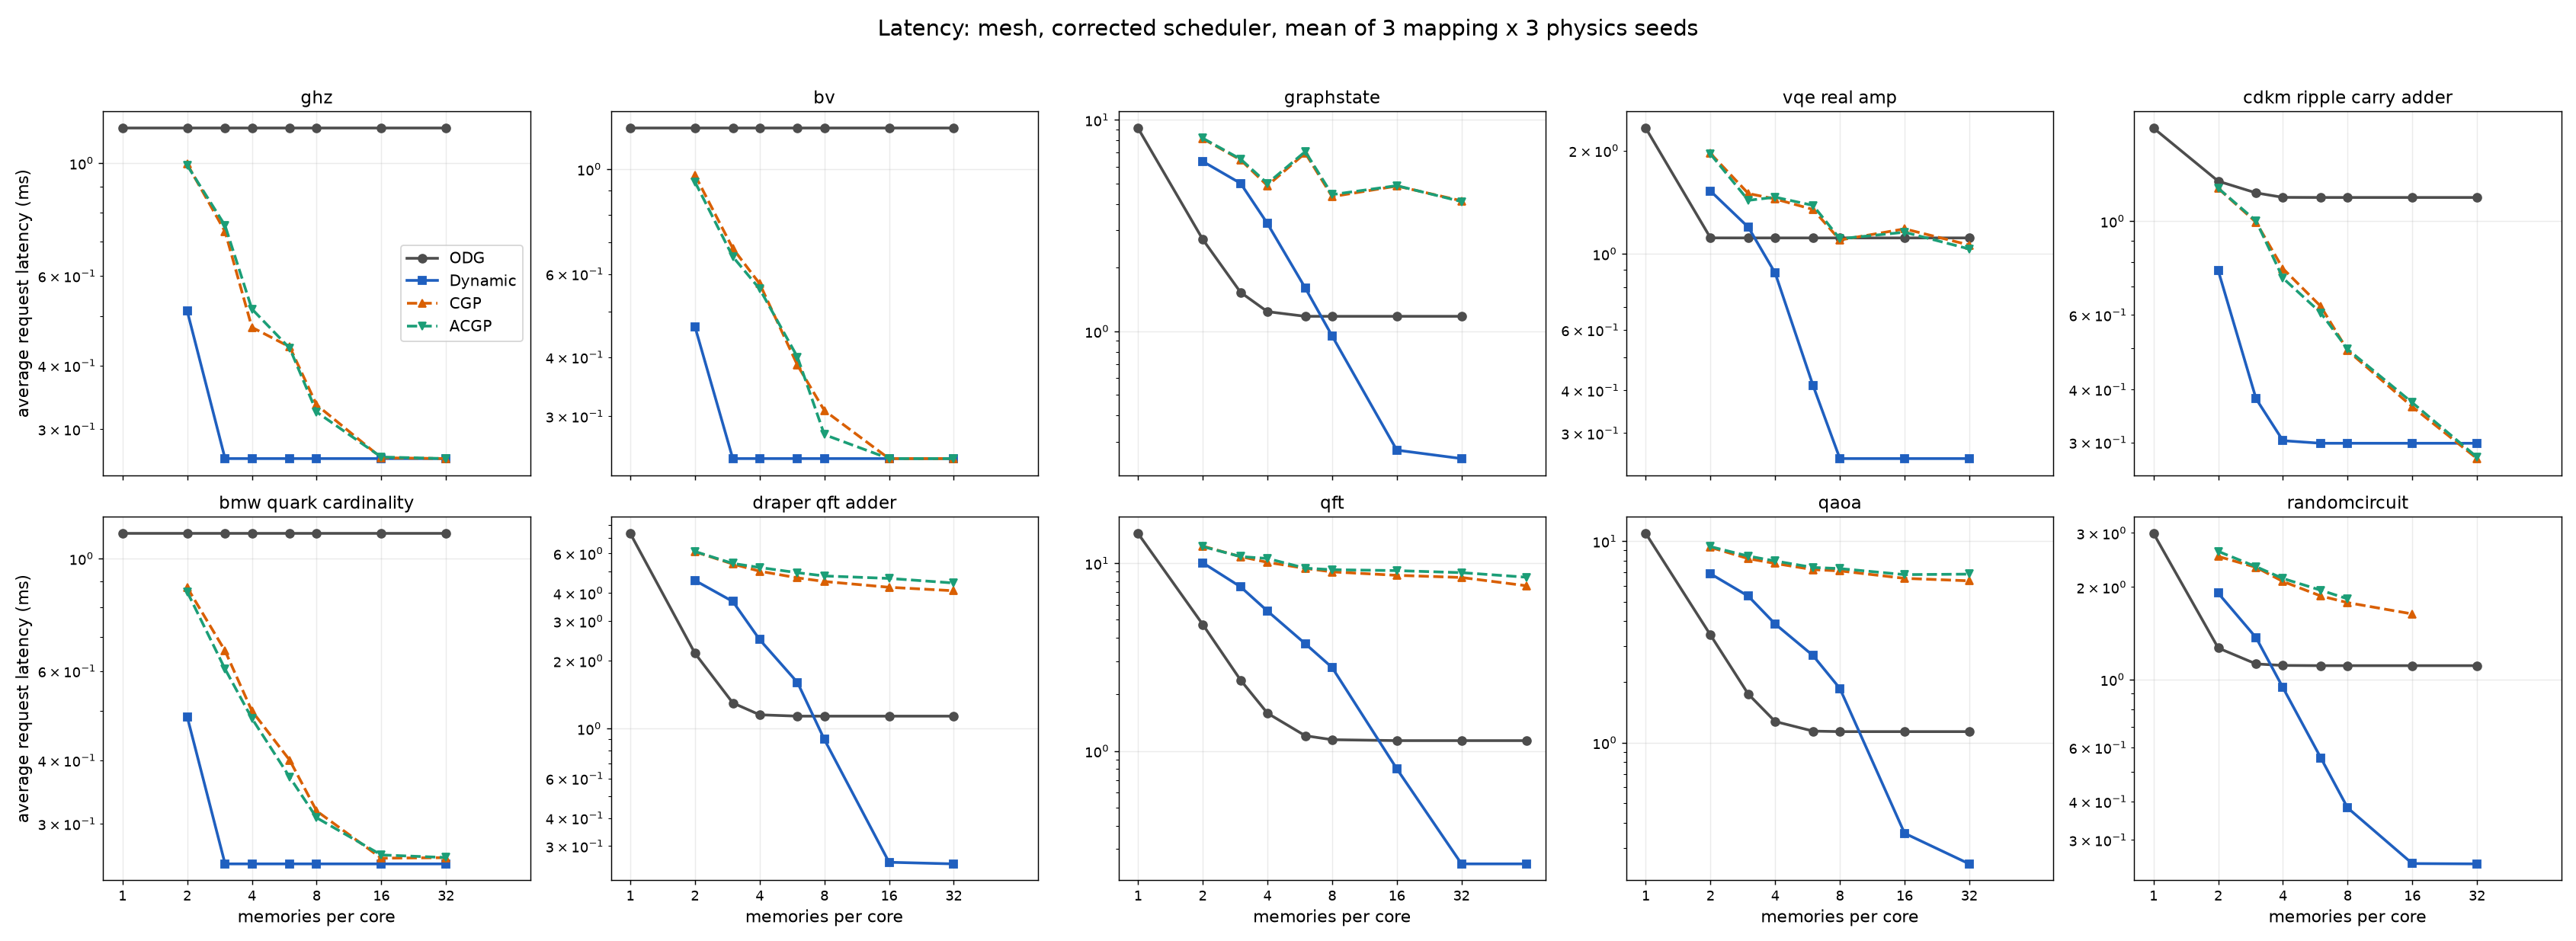
\includegraphics[width=\linewidth,height=0.80\textheight,keepaspectratio]{fp_mesh_latency.png}
\caption{Request latency against memories per core, all four policies (log scale). Mesh, corrected scheduler, mean of three mapping seeds of the mean of three physics seeds; CGP and ACGP cache at most memories$-1$ pairs per core.}
\label{fig:fp-mesh-lat}
\end{figure}
\end{landscape}

\begin{table}[H]
\centering\small
\resizebox{\ifdim\width>\linewidth\linewidth\else\width\fi}{!}{%
\begin{tabular}{@{}lrrrr@{}}
\toprule
Workload & ODG & Dynamic & CGP & ACGP \\
\midrule
GHZ & 1.17 & 0.26 & 0.48 & 0.52 \\
Bernstein--Vazirani & 1.22 & 0.24 & 0.57 & 0.56 \\
BMW/QUARK cardinality & 1.12 & 0.25 & 0.50 & 0.48 \\
VQE real amplitudes & 1.11 & 0.88 & 1.44 & 1.46 \\
CDKM ripple-carry adder & 1.14 & 0.30 & 0.77 & 0.73 \\
Graph state & 1.24 & 3.23 & 4.88 & 5.00 \\
Draper QFT adder & 1.15 & 2.48 & 5.00 & 5.19 \\
QAOA & 1.27 & 3.88 & 7.75 & 7.97 \\
QFT & 1.59 & 5.57 & 10.11 & 10.60 \\
\bottomrule
\end{tabular}}
\caption{Request latency (ms), mesh, 4 memories per core (modelled), mean of three mapping seeds of the mean of three physics seeds.}
\label{tab:fp-mesh-lat-4}
\end{table}

Figure~\ref{fig:fp-mesh-lat} and Table~\ref{tab:fp-mesh-lat-4} give the picture on the mesh. Three results stand out.
\begin{itemize}
  \item \textbf{Dynamic is the fastest of the three pre-generation policies at every memory count from two on, on every benchmark} except one cell (CDKM adder at $32$ memories, where CGP and ACGP are $0.27$ against dynamic's $0.30$\,ms; Table~\ref{tab:fp-mesh-where}).
    At four memories the better of CGP and ACGP takes $1.5$ to $2.4$ times dynamic's latency on the mesh and $1.9$ to $2.5$ times on the torus.
  \item \textbf{Against ODG, dynamic wins on five of the nine benchmarks at the modelled four memories and loses on four.} It wins on BMW, Bernstein--Vazirani, GHZ, the CDKM adder and VQE, and at $32$ memories it is $74$ to $80\%$ faster than ODG on all nine
    (ODG's floor is the generation time of about a millisecond, a ready pair needs a quarter of that); on four of the five it is faster from two memories on.
    It loses on QFT, QAOA, Draper and graph state at two to four memories and overtakes ODG from eight memories on Draper and graph state and from sixteen on QAOA and QFT (Tables~\ref{tab:fp-mesh-gain} and~\ref{tab:fp-mesh-where}).
    The cause is Chapter~\ref{ch:why-dynamic}.
  \item \textbf{CGP and ACGP beat ODG only where ODG is already at its floor.} They are faster than ODG at every memory count on BMW, Bernstein--Vazirani, GHZ and the CDKM adder, and on VQE at some, but \emph{never} on QFT, QAOA, Draper or graph state: at four memories
    they take $4.9$ to $10.6$\,ms on those four against $1.2$ to $1.6$\,ms for ODG. Their wait barely improves with memory.
\end{itemize}
ACGP is not measurably better than CGP: their latencies differ by a median of $2.5\%$ on the mesh and $1.9\%$ on the torus (at most $11\%$ and $14\%$), and their waste by under two points. Why the adaptation has so little effect was not investigated.
\begin{table}[H]
\centering\small
\resizebox{\ifdim\width>\linewidth\linewidth\else\width\fi}{!}{%
\begin{tabular}{@{}lrrrr@{}}
\toprule
Workload & ODG & Dynamic & CGP & ACGP \\
\midrule
GHZ & 1.17 & 0.51 & 1.00 & 0.99 \\
Bernstein--Vazirani & 1.22 & 0.46 & 0.97 & 0.94 \\
BMW/QUARK cardinality & 1.12 & 0.49 & 0.88 & 0.86 \\
VQE real amplitudes & 1.11 & 1.52 & 1.96 & 1.95 \\
CDKM ripple-carry adder & 1.24 & 0.76 & 1.19 & 1.20 \\
Graph state & 2.72 & 6.36 & 8.15 & 8.19 \\
Draper QFT adder & 2.16 & 4.55 & 6.10 & 6.11 \\
QAOA & 3.42 & 6.89 & 9.31 & 9.39 \\
QFT & 4.72 & 10.06 & 12.34 & 12.27 \\
\bottomrule
\end{tabular}}
\caption{Request latency (ms), mesh, 2 memories per core (modelled), mean of three mapping seeds of the mean of three physics seeds.}
\label{tab:fp-mesh-lat-2}
\end{table}

\begin{table}[H]
\centering\small
\resizebox{\ifdim\width>\linewidth\linewidth\else\width\fi}{!}{%
\begin{tabular}{@{}lrrrrrrr@{}}
\toprule
Workload & 2 & 3 & 4 & 6$^*$ & 8$^*$ & 16$^*$ & 32$^*$ \\
\midrule
GHZ & 56\% & 78\% & 78\% & 78\% & 78\% & 78\% & 78\% \\
Bernstein--Vazirani & 62\% & 80\% & 80\% & 80\% & 80\% & 80\% & 80\% \\
BMW/QUARK cardinality & 56\% & 78\% & 78\% & 78\% & 78\% & 78\% & 78\% \\
VQE real amplitudes & -37\% & -7\% & 21\% & 63\% & 77\% & 77\% & 77\% \\
CDKM ripple-carry adder & 39\% & 67\% & 73\% & 74\% & 74\% & 74\% & 74\% \\
Graph state & -134\% & -228\% & -161\% & -36\% & 19\% & 77\% & 79\% \\
Draper QFT adder & -111\% & -182\% & -116\% & -41\% & 21\% & 78\% & 78\% \\
QAOA & -101\% & -207\% & -205\% & -137\% & -64\% & 69\% & 78\% \\
QFT & -113\% & -214\% & -250\% & -209\% & -142\% & 29\% & 78\% \\
Random circuit & -51\% & -22\% & 15\% & 50\% & 66\% & 77\% & 77\% \\
\bottomrule
\end{tabular}}
\caption{Latency gain of dynamic over on-demand, $(\text{ODG}-\text{Dyn.})/\text{ODG}$, mesh; negative means dynamic is slower. Budgets marked $^*$ are counterfactual.}
\label{tab:fp-mesh-gain}
\end{table}

\begin{table}[H]
\centering\small
\resizebox{\ifdim\width>\linewidth\linewidth\else\width\fi}{!}{%
\begin{tabular}{@{}lcccrrrr@{}}
\toprule
Workload & Dynamic beats ODG from (memories) & vs CGP win/tie/loss & vs ACGP win/tie/loss & Fidelity Dyn. & CGP & ACGP & ODG \\
\midrule
GHZ & 2 & 6/1/0 & 6/1/0 & 0.925 & 0.877 & 0.878 & 0.950 \\
Bernstein--Vazirani & 2 & 5/2/0 & 5/2/0 & 0.927 & 0.868 & 0.865 & 0.950 \\
BMW/QUARK cardinality & 2 & 7/0/0 & 7/0/0 & 0.925 & 0.872 & 0.870 & 0.950 \\
VQE real amplitudes & 4 & 7/0/0 & 7/0/0 & 0.916 & 0.899 & 0.899 & 0.950 \\
CDKM ripple-carry adder & 2 & 6/0/1 & 6/0/1 & 0.923 & 0.913 & 0.912 & 0.950 \\
Graph state & 8 & 7/0/0 & 7/0/0 & 0.919 & 0.900 & 0.900 & 0.950 \\
Draper QFT adder & 8 & 7/0/0 & 7/0/0 & 0.922 & 0.903 & 0.902 & 0.950 \\
QAOA & 16 & 7/0/0 & 7/0/0 & 0.925 & 0.905 & 0.904 & 0.950 \\
QFT & 16 & 8/0/0 & 8/0/0 & 0.927 & 0.908 & 0.905 & 0.950 \\
Random circuit & 4 & 6/0/0 & 5/0/0 & 0.913 & 0.899 & 0.898 & 0.950 \\
\bottomrule
\end{tabular}}
\caption{Where dynamic lies, mesh. Column~2: the smallest memory count from which dynamic has lower latency than on-demand ($^\dagger$: with at least one later count where it does not). Columns~3--4: over the memory counts run for both policies (2 to 32; QFT also 64), the number at which dynamic has lower latency, equal latency (the floor reached when nothing waits) or higher latency than CGP and than ACGP. Columns~5--8: delivered fidelity at four memories.}
\label{tab:fp-mesh-where}
\end{table}

\begin{table}[H]
\centering\small
\resizebox{\ifdim\width>\linewidth\linewidth\else\width\fi}{!}{%
\begin{tabular}{@{}rrrrr@{}}
\toprule
Mem. & ODG & Dynamic & CGP & ACGP \\
\midrule
1 & 9 & 0 & 0 & 0 \\
2 & 5 & 4 & 0 & 0 \\
3 & 5 & 4 & 0 & 0 \\
4 & 4 & 5 & 0 & 0 \\
6 & 4 & 5 & 0 & 0 \\
8 & 2 & 7 & 0 & 0 \\
16 & 0 & 8 & 0 & 1 \\
32 & 0 & 6 & 1 & 2 \\
\bottomrule
\end{tabular}}
\caption{Mesh: number of benchmarks (of ten) on which each policy has the lowest latency at each memory count (a policy is counted only where it was run; dynamic, CGP and ACGP start at two memories).}
\label{tab:fp-mesh-best}
\end{table}


\section{Delivered fidelity}
\clearpage\newgeometry{margin=12mm}\begin{landscape}
\begin{figure}[p]
\centering
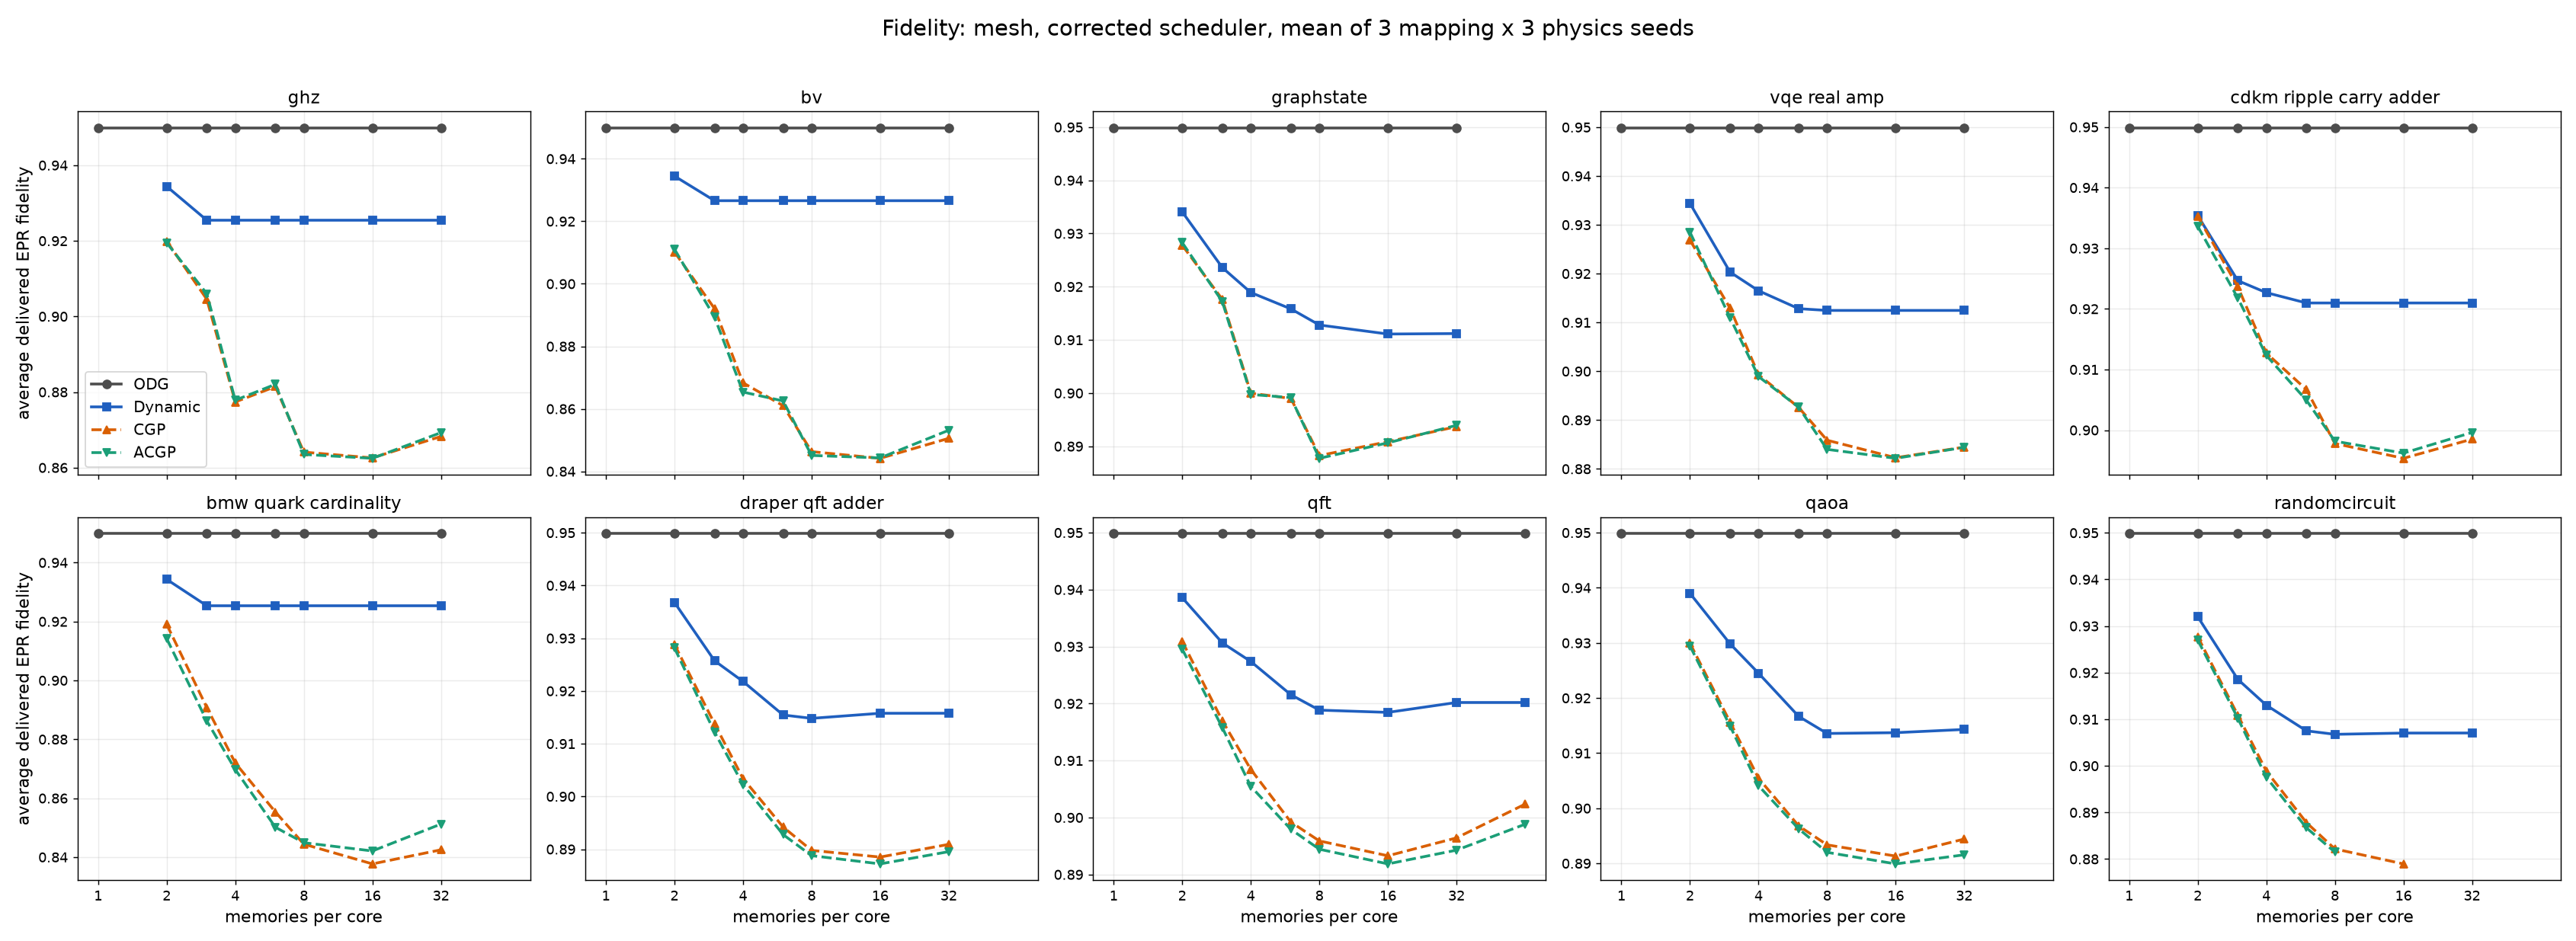
\includegraphics[width=\linewidth,height=0.82\textheight,keepaspectratio]{fp_mesh_fidelity.png}
\caption{Delivered EPR fidelity against memories per core. Mesh, corrected scheduler, mean of three mapping seeds of the mean of three physics seeds; CGP and ACGP cache at most memories$-1$ pairs per core.}
\label{fig:fp-mesh-fid}
\end{figure}
\end{landscape}\clearpage\restoregeometry

\begin{table}[H]
\centering\small
\resizebox{\ifdim\width>\linewidth\linewidth\else\width\fi}{!}{%
\begin{tabular}{@{}lrrrr@{}}
\toprule
Workload & ODG & Dynamic & CGP & ACGP \\
\midrule
GHZ & 0.9498 & 0.9254 & 0.8774 & 0.8778 \\
Bernstein--Vazirani & 0.9498 & 0.9266 & 0.8683 & 0.8654 \\
BMW/QUARK cardinality & 0.9498 & 0.9253 & 0.8720 & 0.8697 \\
VQE real amplitudes & 0.9498 & 0.9165 & 0.8993 & 0.8989 \\
CDKM ripple-carry adder & 0.9498 & 0.9227 & 0.9127 & 0.9123 \\
Graph state & 0.9498 & 0.9189 & 0.9000 & 0.8997 \\
Draper QFT adder & 0.9498 & 0.9218 & 0.9034 & 0.9022 \\
QAOA & 0.9498 & 0.9245 & 0.9054 & 0.9041 \\
QFT & 0.9498 & 0.9274 & 0.9084 & 0.9055 \\
Random circuit & 0.9498 & 0.9130 & 0.8989 & 0.8976 \\
\bottomrule
\end{tabular}}
\caption{Delivered EPR fidelity, mesh, 4 memories per core (modelled), mean of three mapping seeds of the mean of three physics seeds.}
\label{tab:fp-mesh-fid-4}
\end{table}

ODG delivers $0.950$ always. Dynamic's pairs wait in memory and decohere: its fidelity is $0.911$ to $0.939$ over all budgets ($0.916$ to $0.927$ at four memories) and falls from two to $32$ memories on every benchmark, as the compiler bank grows. CGP and ACGP are lower and more
variable, $0.838$ to $0.935$ over all budgets ($0.865$ to $0.913$ at four memories), presumably because their pairs age longer before use (the age of CGP and ACGP pairs was not measured). Dynamic's pairs are
better by $0.01$ to $0.06$ at four memories, but never as good as on-demand pairs. (These figures use ACE's coherence time of one second; under the group's multi-core paper's $1$\,ms every cached pair would expire, Chapter~\ref{ch:exp1}.)

\section{Wasted pairs and readiness}
\clearpage\newgeometry{margin=12mm}\begin{landscape}
\begin{figure}[p]
\centering
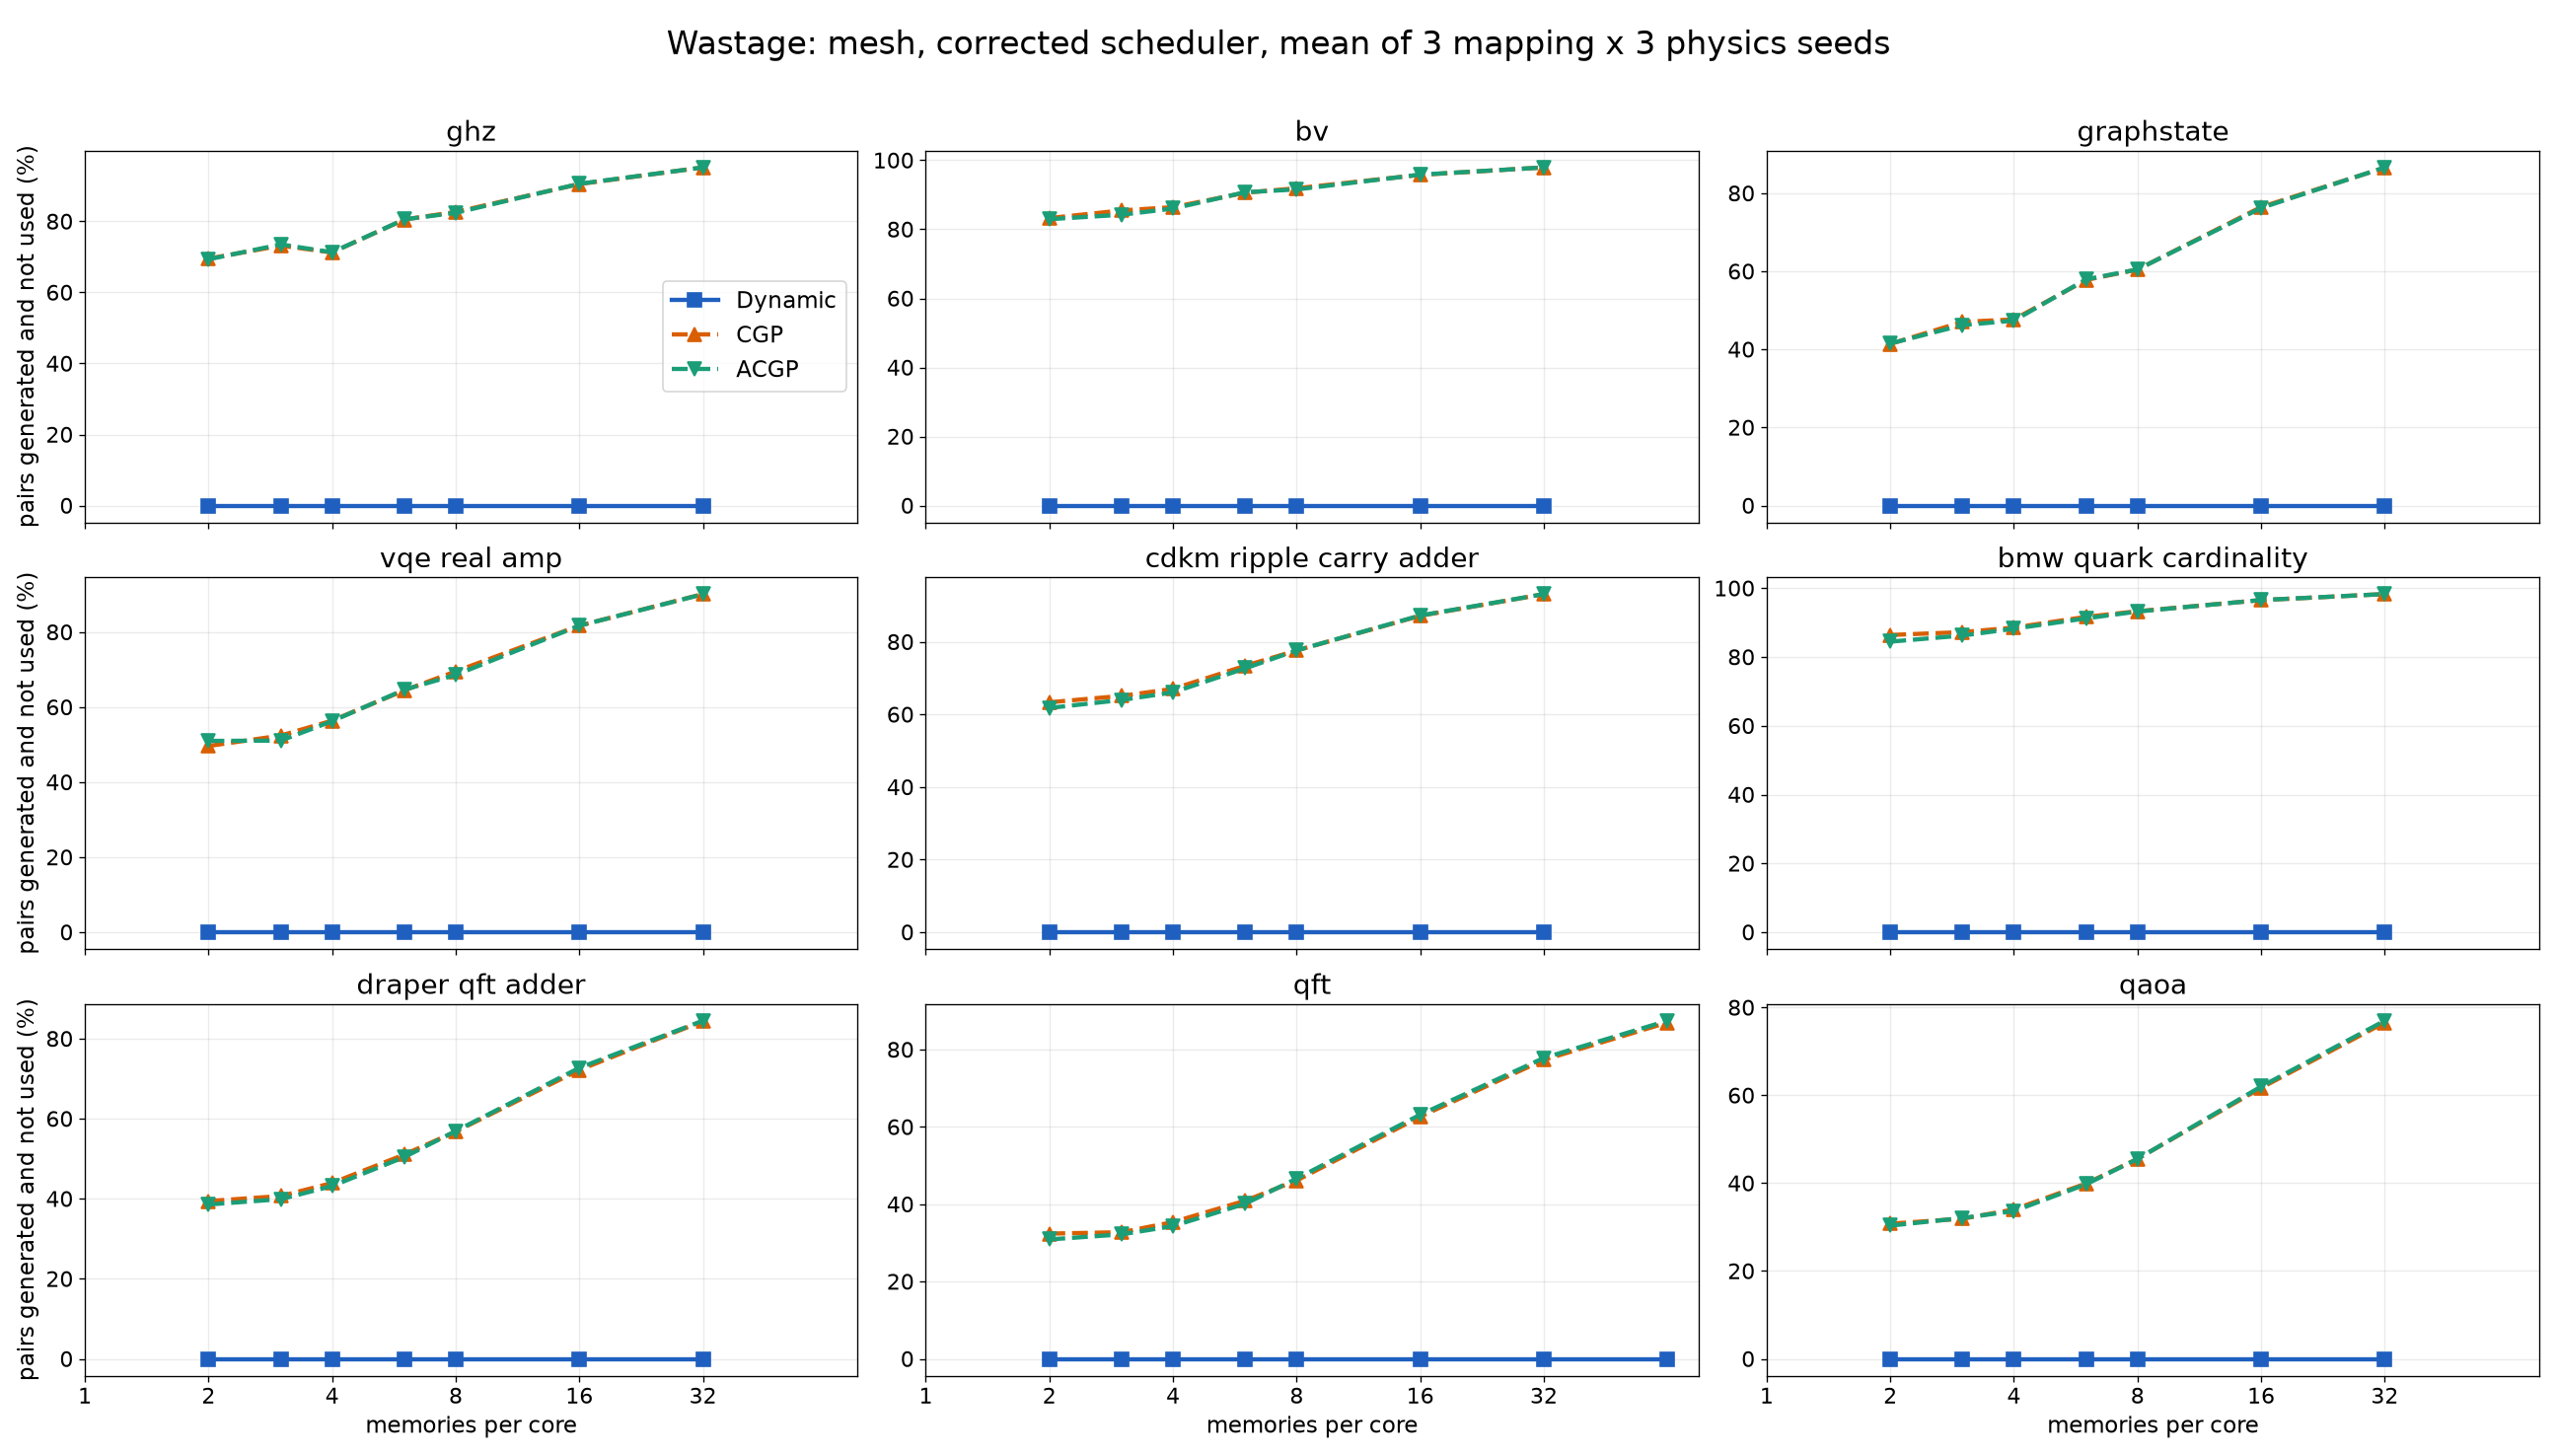
\includegraphics[width=\linewidth,height=0.82\textheight,keepaspectratio]{fp_mesh_waste.png}
\caption{Pairs generated and not used by the end of the run, as a percentage of pairs generated (dynamic, CGP, ACGP). Mesh, corrected scheduler, mean of three mapping seeds of the mean of three physics seeds; CGP and ACGP cache at most memories$-1$ pairs per core.}
\label{fig:fp-mesh-waste}
\end{figure}
\end{landscape}\clearpage\restoregeometry

\begin{table}[H]
\centering\small
\resizebox{\ifdim\width>\linewidth\linewidth\else\width\fi}{!}{%
\begin{tabular}{@{}lrrr@{}}
\toprule
Workload & Dynamic & CGP & ACGP \\
\midrule
GHZ & 0.0 & 71.3 & 71.3 \\
Bernstein--Vazirani & 0.0 & 86.4 & 86.0 \\
BMW/QUARK cardinality & 0.0 & 88.6 & 88.2 \\
VQE real amplitudes & 0.0 & 56.4 & 56.3 \\
CDKM ripple-carry adder & 0.0 & 67.1 & 66.1 \\
Graph state & 0.0 & 47.7 & 47.4 \\
Draper QFT adder & 0.0 & 43.9 & 43.2 \\
QAOA & 0.0 & 34.0 & 33.6 \\
QFT & 0.0 & 35.4 & 34.3 \\
\bottomrule
\end{tabular}}
\caption{Pairs generated and never used (\%), mesh, 4 memories per core (modelled), mean of three mapping seeds of the mean of three physics seeds.}
\label{tab:fp-mesh-waste-4}
\end{table}

Dynamic wastes no pair on the mesh (every prepared pair is used). CGP and ACGP waste $34$ to $89\%$ of their pairs at four memories on the mesh, and more with more memory
($31\%$ on QFT at two memories, $78\%$ at $32$): they make pairs for neighbours drawn at random, and a pair nobody uses before its window ends is lost. The percentage depends on the size of the workload: at four memories it is highest on BMW, Bernstein--Vazirani, GHZ
and the CDKM adder ($24$ to $456$ requests) and lowest on QAOA, QFT and Draper ($1\,310$ to $3\,068$ requests), so it is comparable only within a benchmark. Cached pairs, used or not, are also what block requests (Chapter~\ref{ch:why-dynamic}).
\begin{landscape}
\begin{figure}[p]
\centering
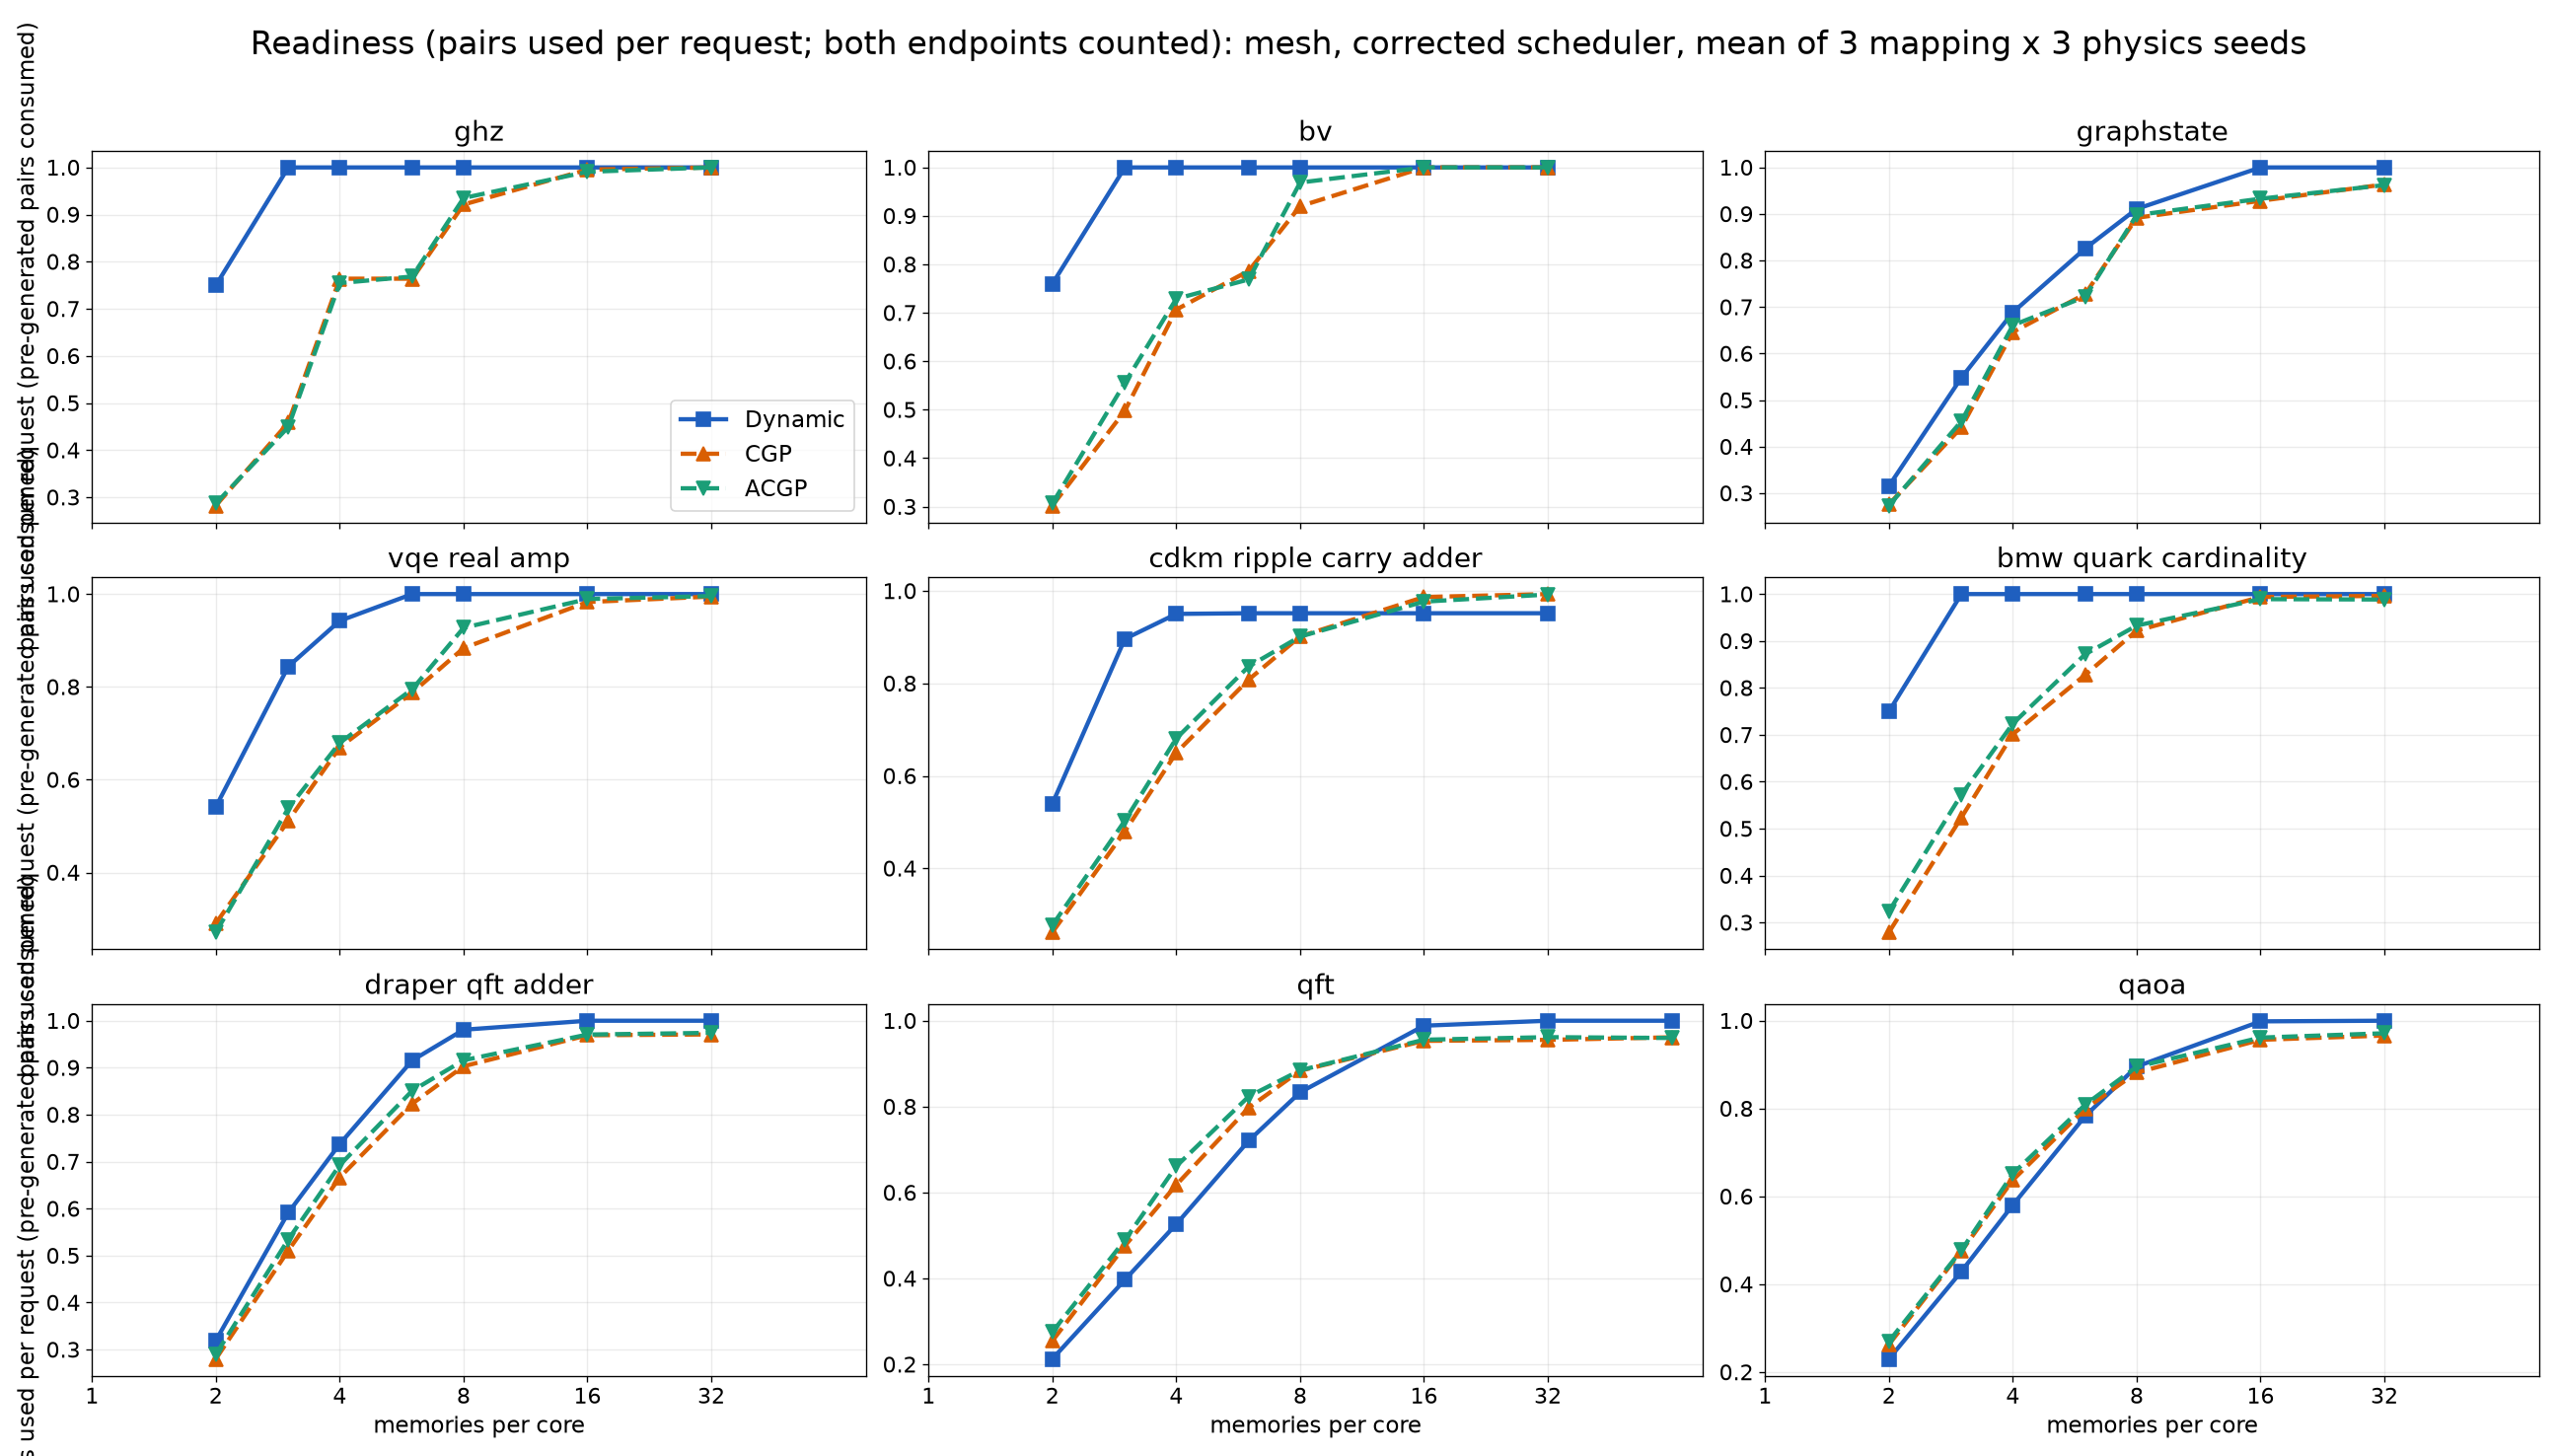
\includegraphics[width=\linewidth,height=0.80\textheight,keepaspectratio]{fp_mesh_readiness.png}
\caption{Pre-generated pairs consumed per request (pairs are counted at both endpoints, so the unit is pairs used divided by twice the requests). Mesh, corrected scheduler, mean of three mapping seeds of the mean of three physics seeds; CGP and ACGP cache at most memories$-1$ pairs per core.}
\label{fig:fp-mesh-ready}
\end{figure}
\end{landscape}

Readiness differs less than one would expect. At four memories dynamic serves $100\%$ of the requests of BMW, Bernstein--Vazirani and GHZ from a ready pair, $94$ to $95\%$ on VQE and the CDKM adder, but only $53$ to $74\%$ on the four congested circuits,
where the planner could not place a preparation for the rest within the compiler's memories (for QFT it placed $1\,330$ of $2\,510$ requests). CGP and ACGP find a cached pair for $62$ to $76\%$ of the requests at four memories --- more than dynamic on QFT and QAOA --- because a cached pair for a link serves any request
on that link, yet they are slower, because a request that has such a pair still has to wait for a memory of its own (Section~\ref{sec:code-reading}).

\section{Waiting}
\begin{landscape}
\begin{figure}[p]
\centering
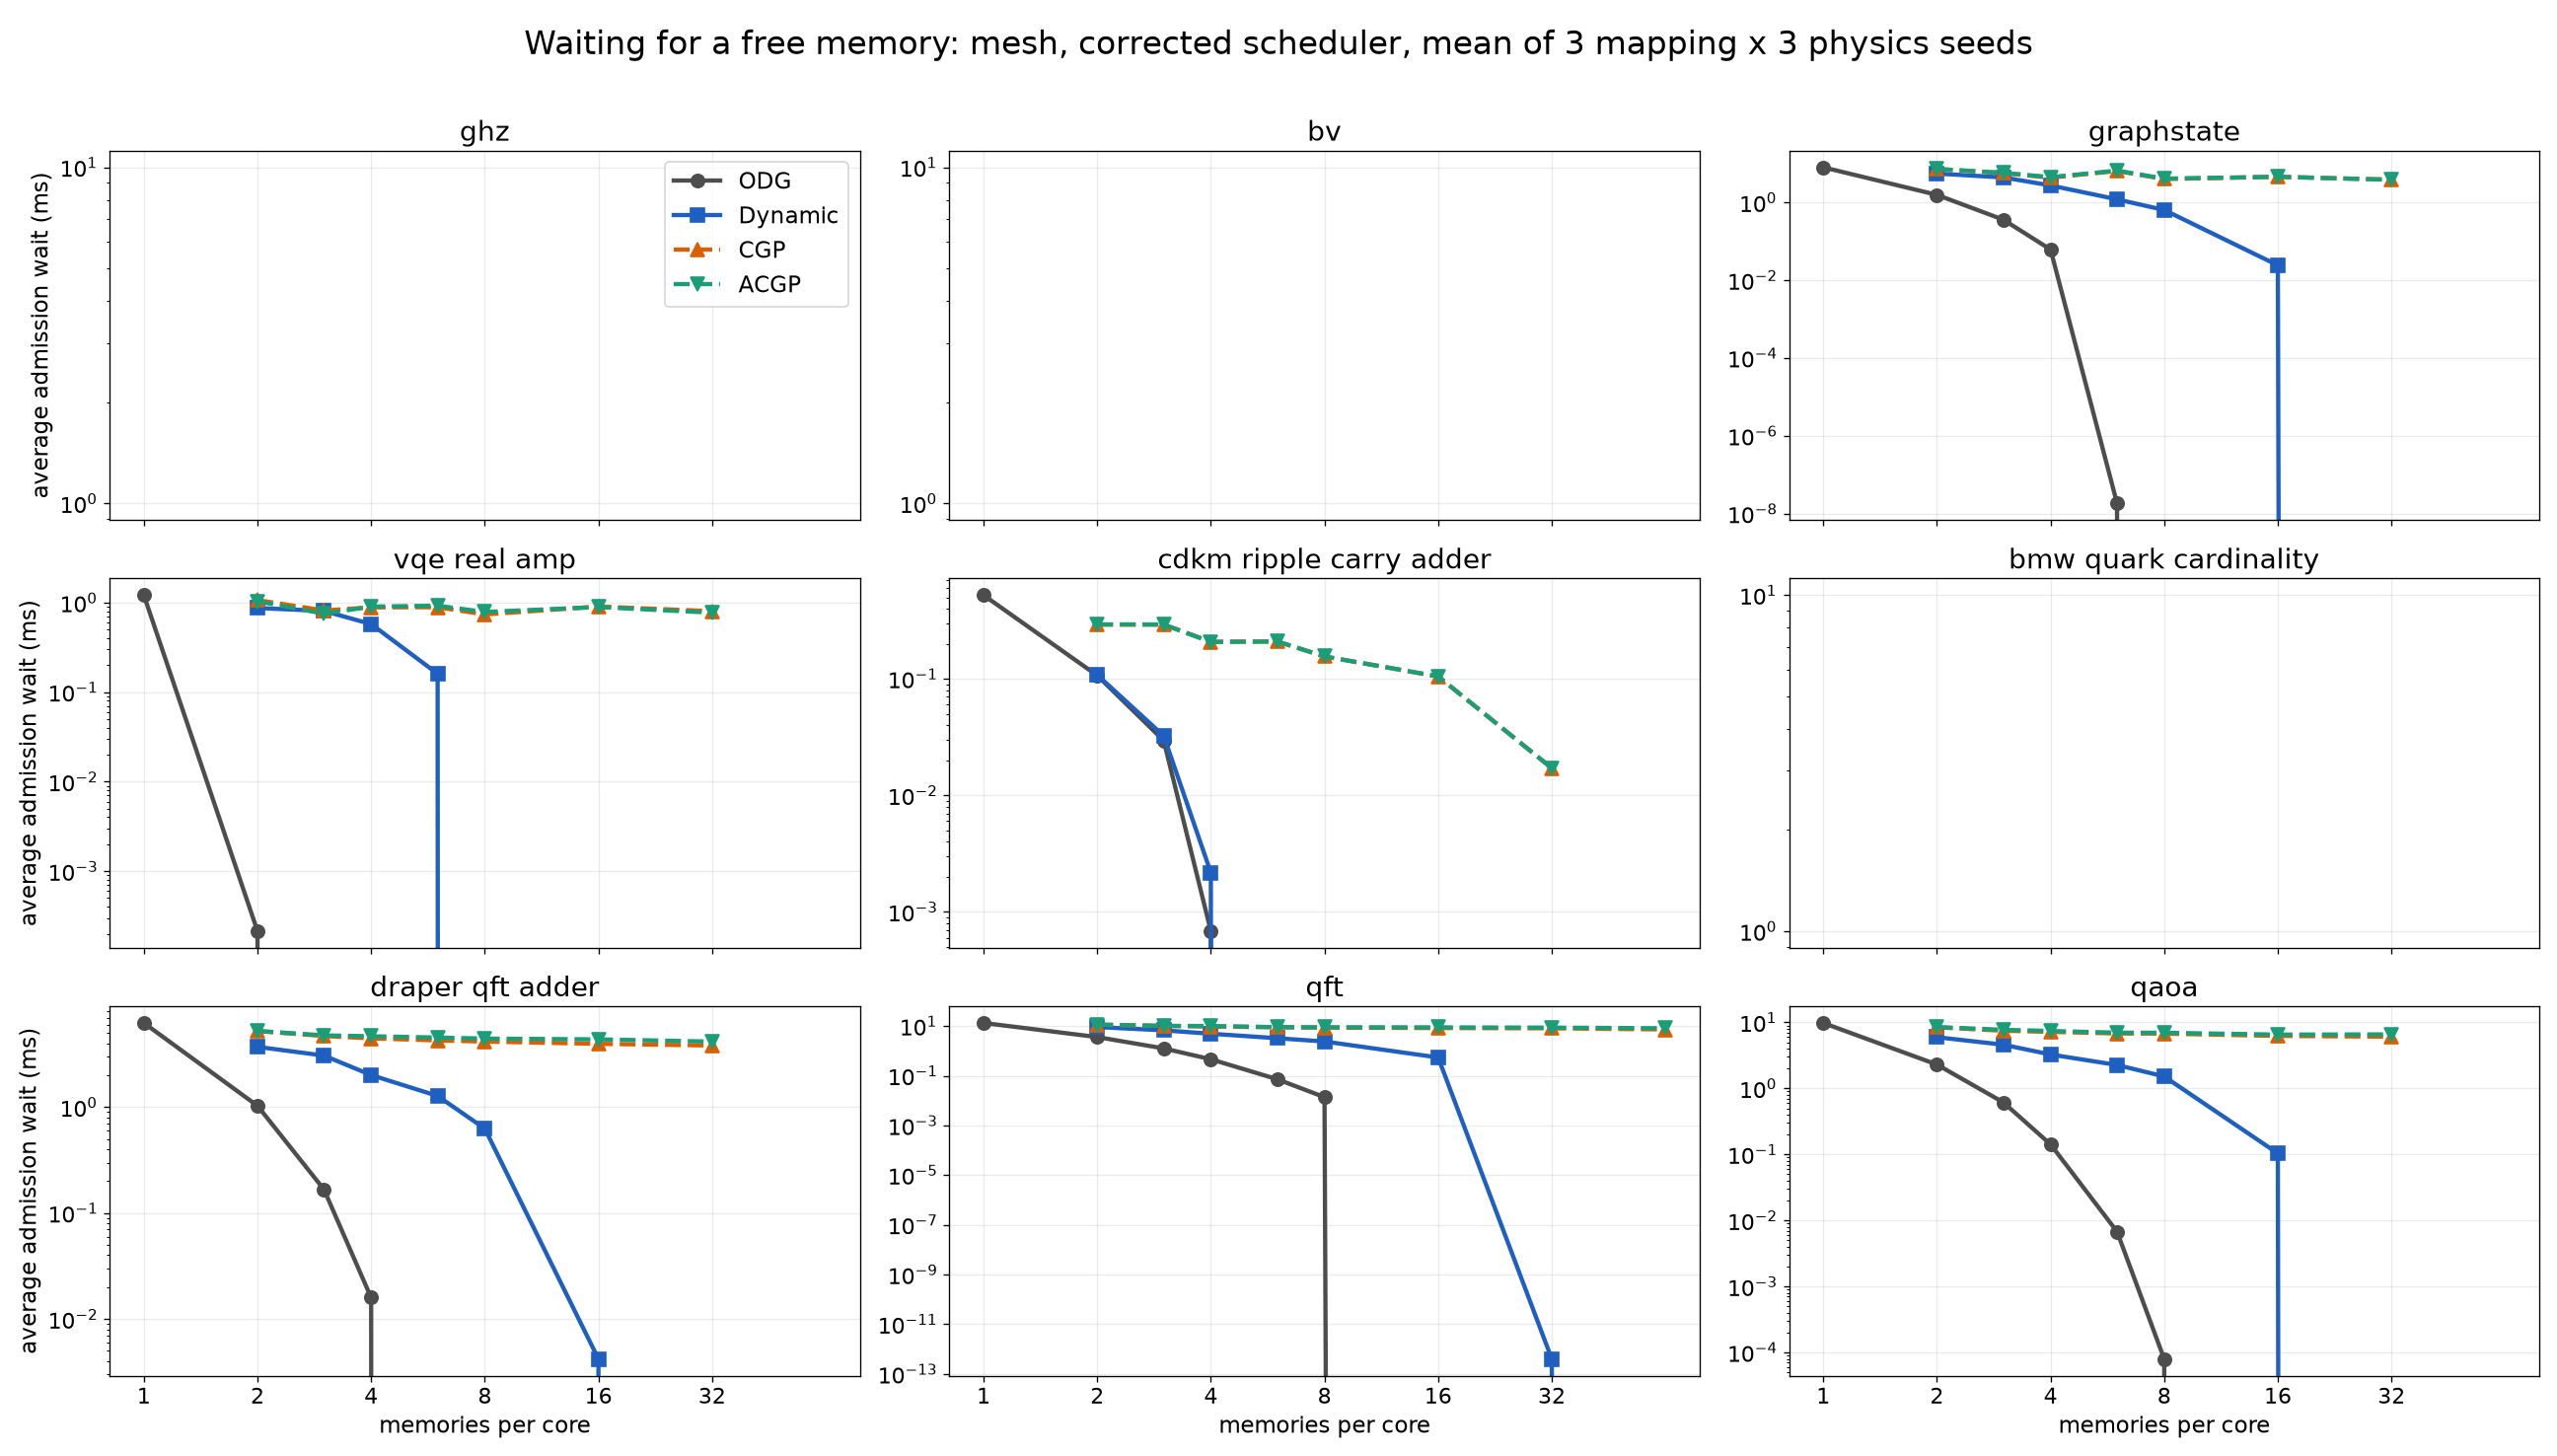
\includegraphics[width=\linewidth,height=0.80\textheight,keepaspectratio]{fp_mesh_wait.png}
\caption{Average wait for a free memory (log scale). Mesh, corrected scheduler, mean of three mapping seeds of the mean of three physics seeds; CGP and ACGP cache at most memories$-1$ pairs per core.}
\label{fig:fp-mesh-wait}
\end{figure}
\end{landscape}

\begin{table}[H]
\centering\small
\resizebox{\ifdim\width>\linewidth\linewidth\else\width\fi}{!}{%
\begin{tabular}{@{}lrrrr@{}}
\toprule
Workload & ODG & Dynamic & CGP & ACGP \\
\midrule
GHZ & 0.00 & 0.00 & 0.00 & 0.00 \\
Bernstein--Vazirani & 0.00 & 0.00 & 0.00 & 0.00 \\
BMW/QUARK cardinality & 0.00 & 0.00 & 0.00 & 0.00 \\
VQE real amplitudes & 0.00 & 0.58 & 0.88 & 0.90 \\
CDKM ripple-carry adder & 0.00 & 0.00 & 0.21 & 0.21 \\
Graph state & 0.06 & 2.73 & 4.33 & 4.46 \\
Draper QFT adder & 0.02 & 2.01 & 4.46 & 4.67 \\
QAOA & 0.14 & 3.27 & 7.20 & 7.42 \\
QFT & 0.46 & 4.91 & 9.54 & 10.06 \\
\bottomrule
\end{tabular}}
\caption{Wait for a free memory (ms), mesh, 4 memories per core (modelled), mean of three mapping seeds of the mean of three physics seeds.}
\label{tab:fp-mesh-wait-4}
\end{table}

Waiting for a free memory is where the policies differ. On the congested circuits at four memories ODG waits $0.02$ to $0.46$\,ms on average, dynamic $2.0$ to $4.9$\,ms and CGP and ACGP $4.3$ to $10.1$\,ms; on the other five circuits nobody waits
more than about a millisecond. The cause is the number of memory cards held by pre-generated pairs (Chapter~\ref{ch:why-dynamic}).

\section{The torus}
\begin{table}[H]
\centering\small
\resizebox{\ifdim\width>\linewidth\linewidth\else\width\fi}{!}{%
\begin{tabular}{@{}lrrrr@{}}
\toprule
Workload & ODG & Dynamic & CGP & ACGP \\
\midrule
GHZ & 1.15 & 0.28 & 0.72 & 0.77 \\
Bernstein--Vazirani & 1.11 & 0.23 & 0.50 & 0.43 \\
BMW/QUARK cardinality & 1.10 & 0.25 & 0.61 & 0.54 \\
VQE real amplitudes & 1.14 & 0.48 & 1.00 & 1.02 \\
CDKM ripple-carry adder & 1.09 & 0.31 & 0.74 & 0.69 \\
Graph state & 1.11 & 1.99 & 4.06 & 4.05 \\
Draper QFT adder & 1.13 & 2.71 & 5.81 & 6.01 \\
QAOA & 1.17 & 3.00 & 6.49 & 6.37 \\
QFT & 1.21 & 3.38 & 7.46 & 7.62 \\
\bottomrule
\end{tabular}}
\caption{Request latency (ms), torus, 4 memories per core (modelled), mean of three mapping seeds of the mean of three physics seeds.}
\label{tab:fp-torus-lat-4}
\end{table}

\begin{table}[H]
\centering\small
\resizebox{\ifdim\width>\linewidth\linewidth\else\width\fi}{!}{%
\begin{tabular}{@{}lrrrrrrr@{}}
\toprule
Workload & 2 & 3 & 4 & 6$^*$ & 8$^*$ & 16$^*$ & 32$^*$ \\
\midrule
GHZ & 68\% & 75\% & 75\% & 75\% & 75\% & 75\% & 75\% \\
Bernstein--Vazirani & 67\% & 79\% & 79\% & 79\% & 79\% & 79\% & 79\% \\
BMW/QUARK cardinality & 66\% & 77\% & 77\% & 77\% & 77\% & 77\% & 77\% \\
VQE real amplitudes & 43\% & 55\% & 58\% & 66\% & 74\% & 76\% & 76\% \\
CDKM ripple-carry adder & 40\% & 66\% & 72\% & 73\% & 73\% & 73\% & 73\% \\
Graph state & -98\% & -131\% & -79\% & -21\% & 44\% & 77\% & 77\% \\
Draper QFT adder & -119\% & -224\% & -141\% & -37\% & 33\% & 77\% & 77\% \\
QAOA & -110\% & -193\% & -157\% & -65\% & 2\% & 77\% & 78\% \\
QFT & -125\% & -219\% & -179\% & -85\% & -3\% & 77\% & 78\% \\
\bottomrule
\end{tabular}}
\caption{Latency gain of dynamic over on-demand, $(\text{ODG}-\text{Dyn.})/\text{ODG}$, torus; negative means dynamic is slower. Budgets marked $^*$ are counterfactual.}
\label{tab:fp-torus-gain}
\end{table}

\begin{table}[H]
\centering\small
\resizebox{\ifdim\width>\linewidth\linewidth\else\width\fi}{!}{%
\begin{tabular}{@{}lcccrrrr@{}}
\toprule
Workload & Dynamic beats ODG from (memories) & vs CGP win/tie/loss & vs ACGP win/tie/loss & Fidelity Dyn. & CGP & ACGP & ODG \\
\midrule
GHZ & 2 & 5/2/0 & 5/2/0 & 0.931 & 0.878 & 0.879 & 0.950 \\
Bernstein--Vazirani & 2 & 6/1/0 & 6/1/0 & 0.930 & 0.871 & 0.870 & 0.950 \\
BMW/QUARK cardinality & 2 & 7/0/0 & 7/0/0 & 0.931 & 0.880 & 0.879 & 0.950 \\
VQE real amplitudes & 2 & 7/0/0 & 7/0/0 & 0.929 & 0.902 & 0.906 & 0.950 \\
CDKM ripple-carry adder & 2 & 7/0/0 & 7/0/0 & 0.925 & 0.919 & 0.916 & 0.950 \\
Graph state & 8 & 7/0/0 & 7/0/0 & 0.919 & 0.894 & 0.894 & 0.950 \\
Draper QFT adder & 8 & 7/0/0 & 7/0/0 & 0.925 & 0.910 & 0.908 & 0.950 \\
QAOA & 8 & 7/0/0 & 7/0/0 & 0.925 & 0.906 & 0.906 & 0.950 \\
QFT & 16 & 8/0/0 & 8/0/0 & 0.928 & 0.910 & 0.909 & 0.950 \\
\bottomrule
\end{tabular}}
\caption{Where dynamic lies, torus. Column~2: the smallest memory count from which dynamic has lower latency than on-demand ($^\dagger$: with at least one later count where it does not). Columns~3--4: over the memory counts run for both policies (2 to 32; QFT also 64), the number at which dynamic has lower latency, equal latency (the floor reached when nothing waits) or higher latency than CGP and than ACGP. Columns~5--8: delivered fidelity at four memories.}
\label{tab:fp-torus-where}
\end{table}

\begin{table}[H]
\centering\small
\resizebox{\ifdim\width>\linewidth\linewidth\else\width\fi}{!}{%
\begin{tabular}{@{}rrrrr@{}}
\toprule
Mem. & ODG & Dynamic & CGP & ACGP \\
\midrule
1 & 9 & 0 & 0 & 0 \\
2 & 4 & 5 & 0 & 0 \\
3 & 4 & 5 & 0 & 0 \\
4 & 4 & 5 & 0 & 0 \\
6 & 4 & 5 & 0 & 0 \\
8 & 1 & 8 & 0 & 0 \\
16 & 0 & 8 & 0 & 1 \\
32 & 0 & 7 & 0 & 2 \\
\bottomrule
\end{tabular}}
\caption{Torus: number of benchmarks (of ten) on which each policy has the lowest latency at each memory count (a policy is counted only where it was run; dynamic, CGP and ACGP start at two memories).}
\label{tab:fp-torus-best}
\end{table}

The ordering is the same on the torus: dynamic is faster than the better of CGP and ACGP on every benchmark at every memory count except ties at the floor (Table~\ref{tab:fp-torus-where}); against ODG it wins on the same five benchmarks at four memories,
loses on QFT, QAOA, Draper and graph state at two to four, and overtakes ODG from eight memories on Draper, graph state and QAOA and from sixteen on QFT. CGP and ACGP beat ODG on BMW, Bernstein--Vazirani, GHZ and the CDKM adder at every
memory count and on VQE from three or four, and never on the other four. Waste is higher on the torus ($34$ to $92\%$ at four memories). The figures for the torus follow.
\clearpage\newgeometry{margin=12mm}\begin{landscape}
\begin{figure}[p]
\centering
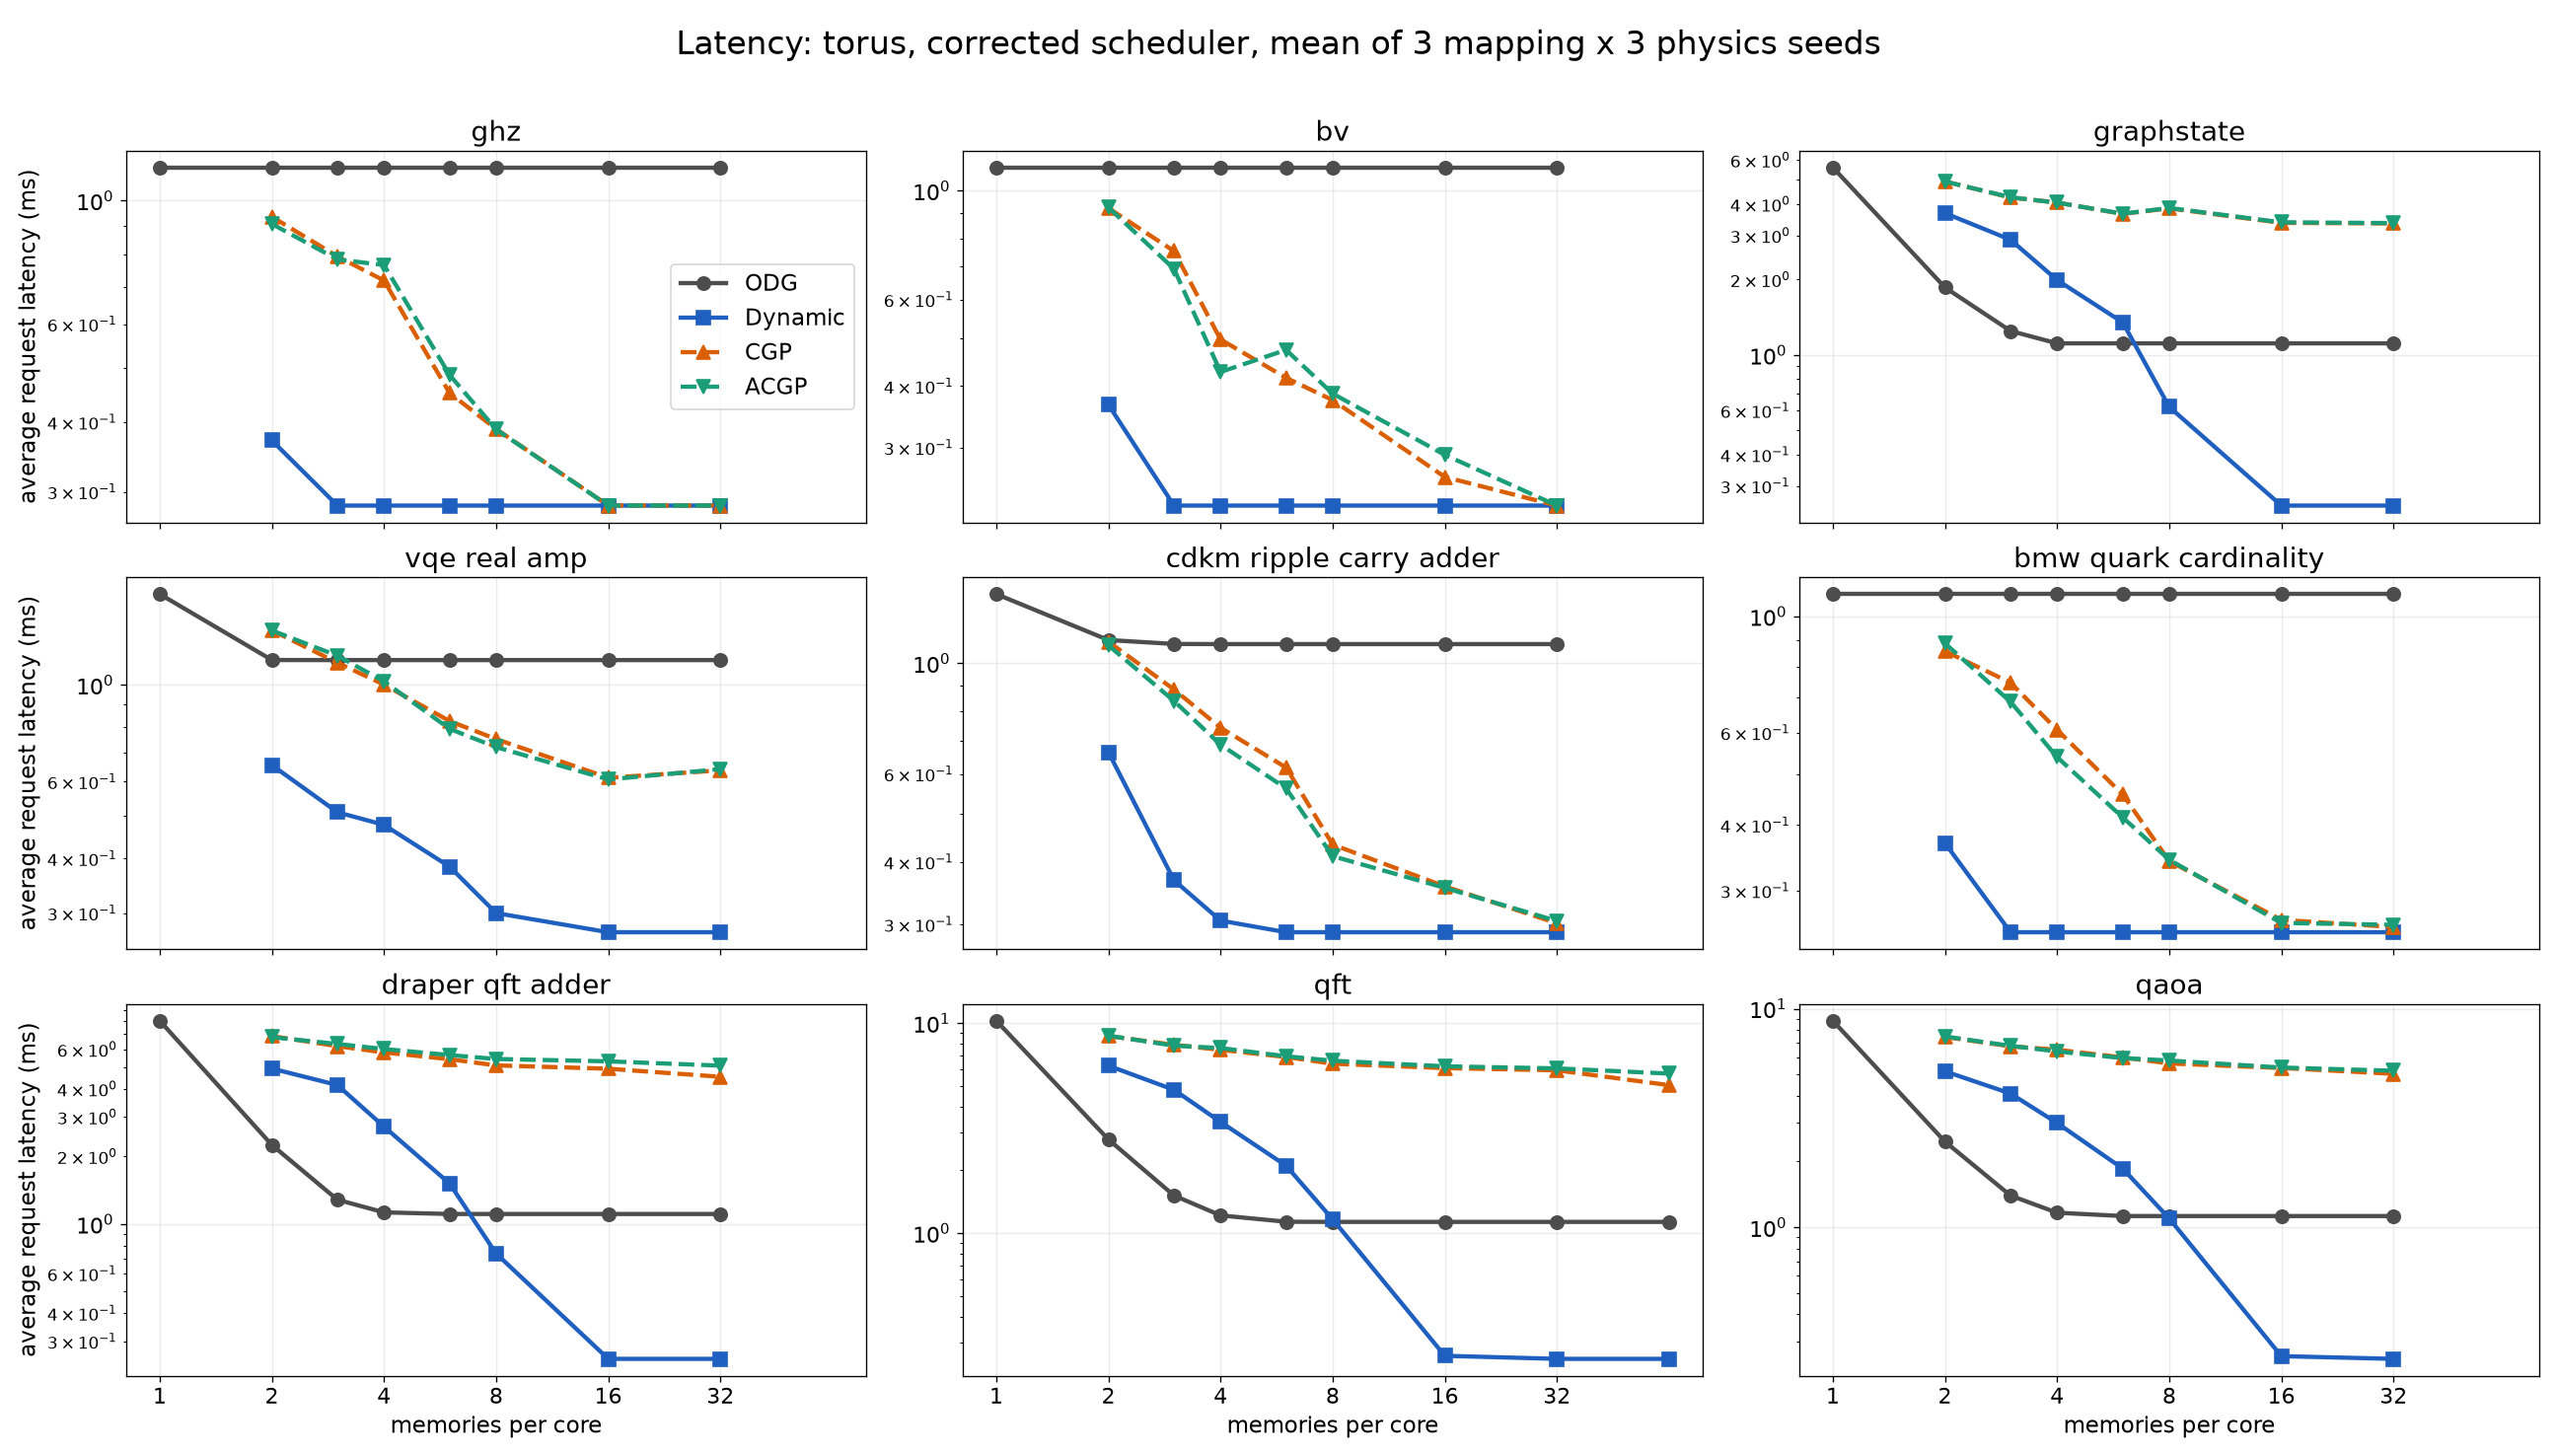
\includegraphics[width=\linewidth,height=0.82\textheight,keepaspectratio]{fp_torus_latency.png}
\caption{Request latency against memories per core, all four policies (log scale). Torus, corrected scheduler, mean of three mapping seeds of the mean of three physics seeds; CGP and ACGP cache at most memories$-1$ pairs per core.}
\label{fig:fp-torus-lat}
\end{figure}
\end{landscape}\clearpage\restoregeometry

\clearpage\newgeometry{margin=12mm}\begin{landscape}
\begin{figure}[p]
\centering
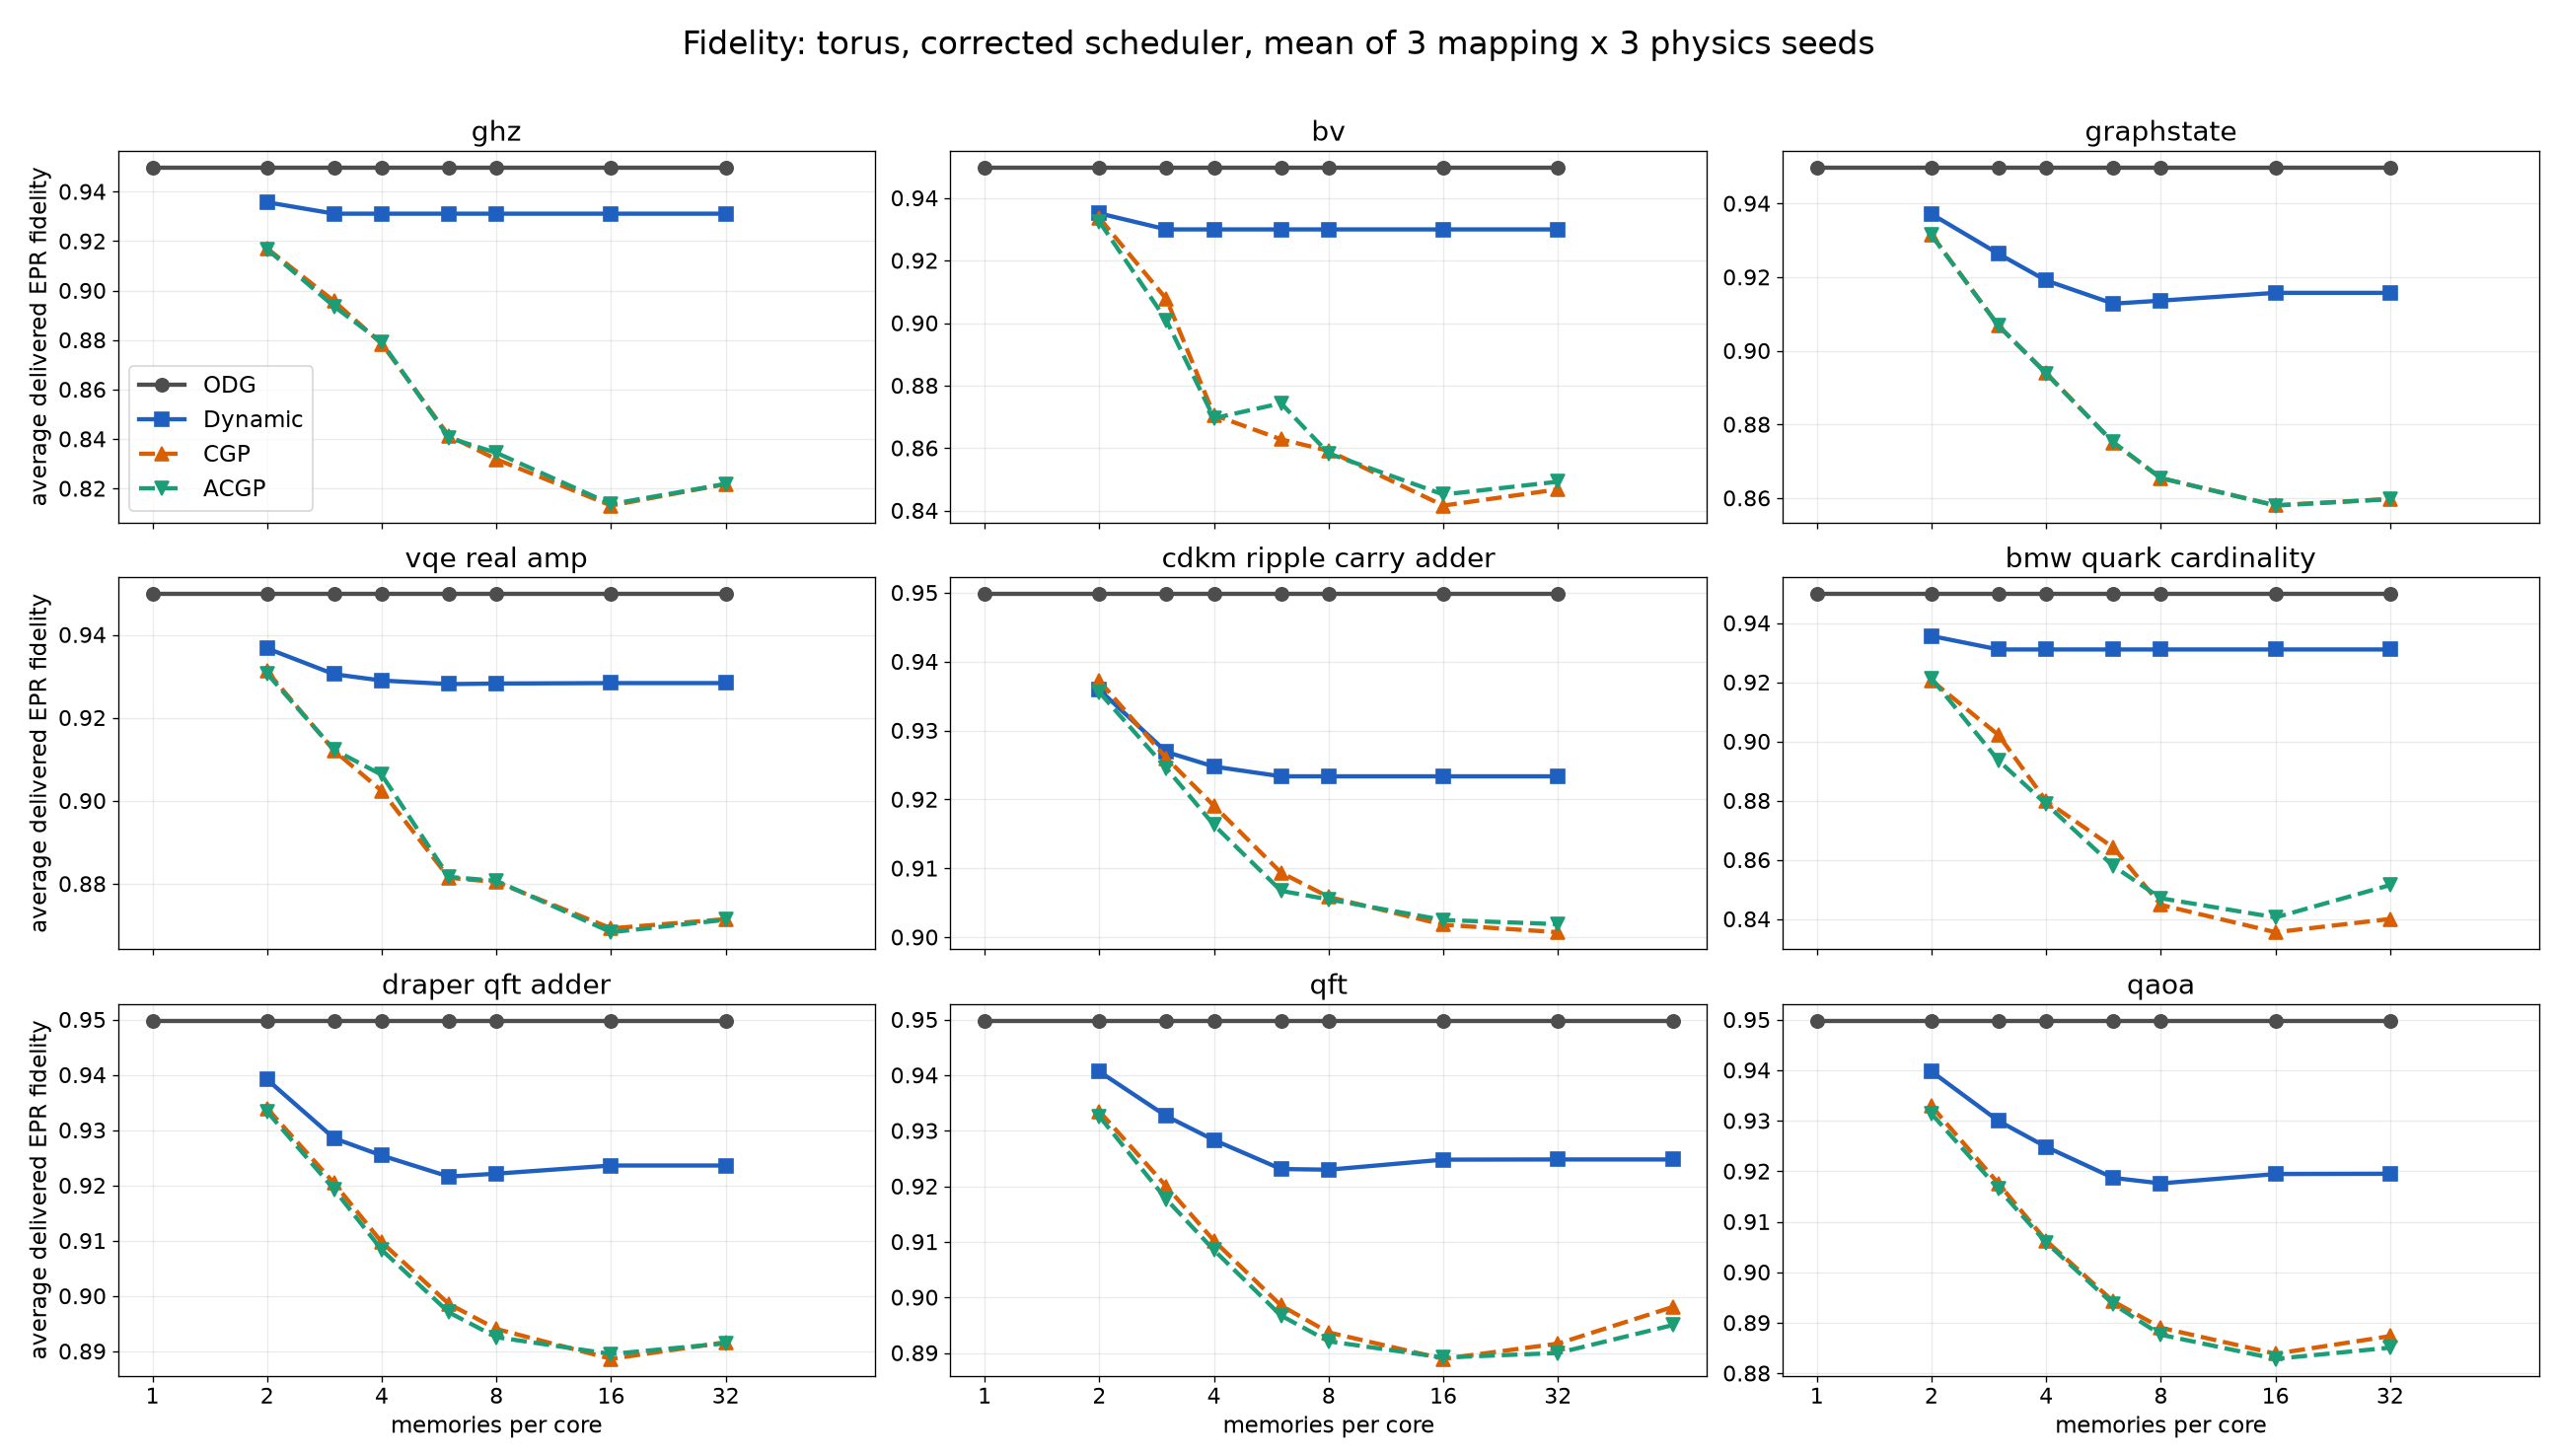
\includegraphics[width=\linewidth,height=0.82\textheight,keepaspectratio]{fp_torus_fidelity.png}
\caption{Delivered EPR fidelity against memories per core. Torus, corrected scheduler, mean of three mapping seeds of the mean of three physics seeds; CGP and ACGP cache at most memories$-1$ pairs per core.}
\label{fig:fp-torus-fid}
\end{figure}
\end{landscape}\clearpage\restoregeometry

\clearpage\newgeometry{margin=12mm}\begin{landscape}
\begin{figure}[p]
\centering
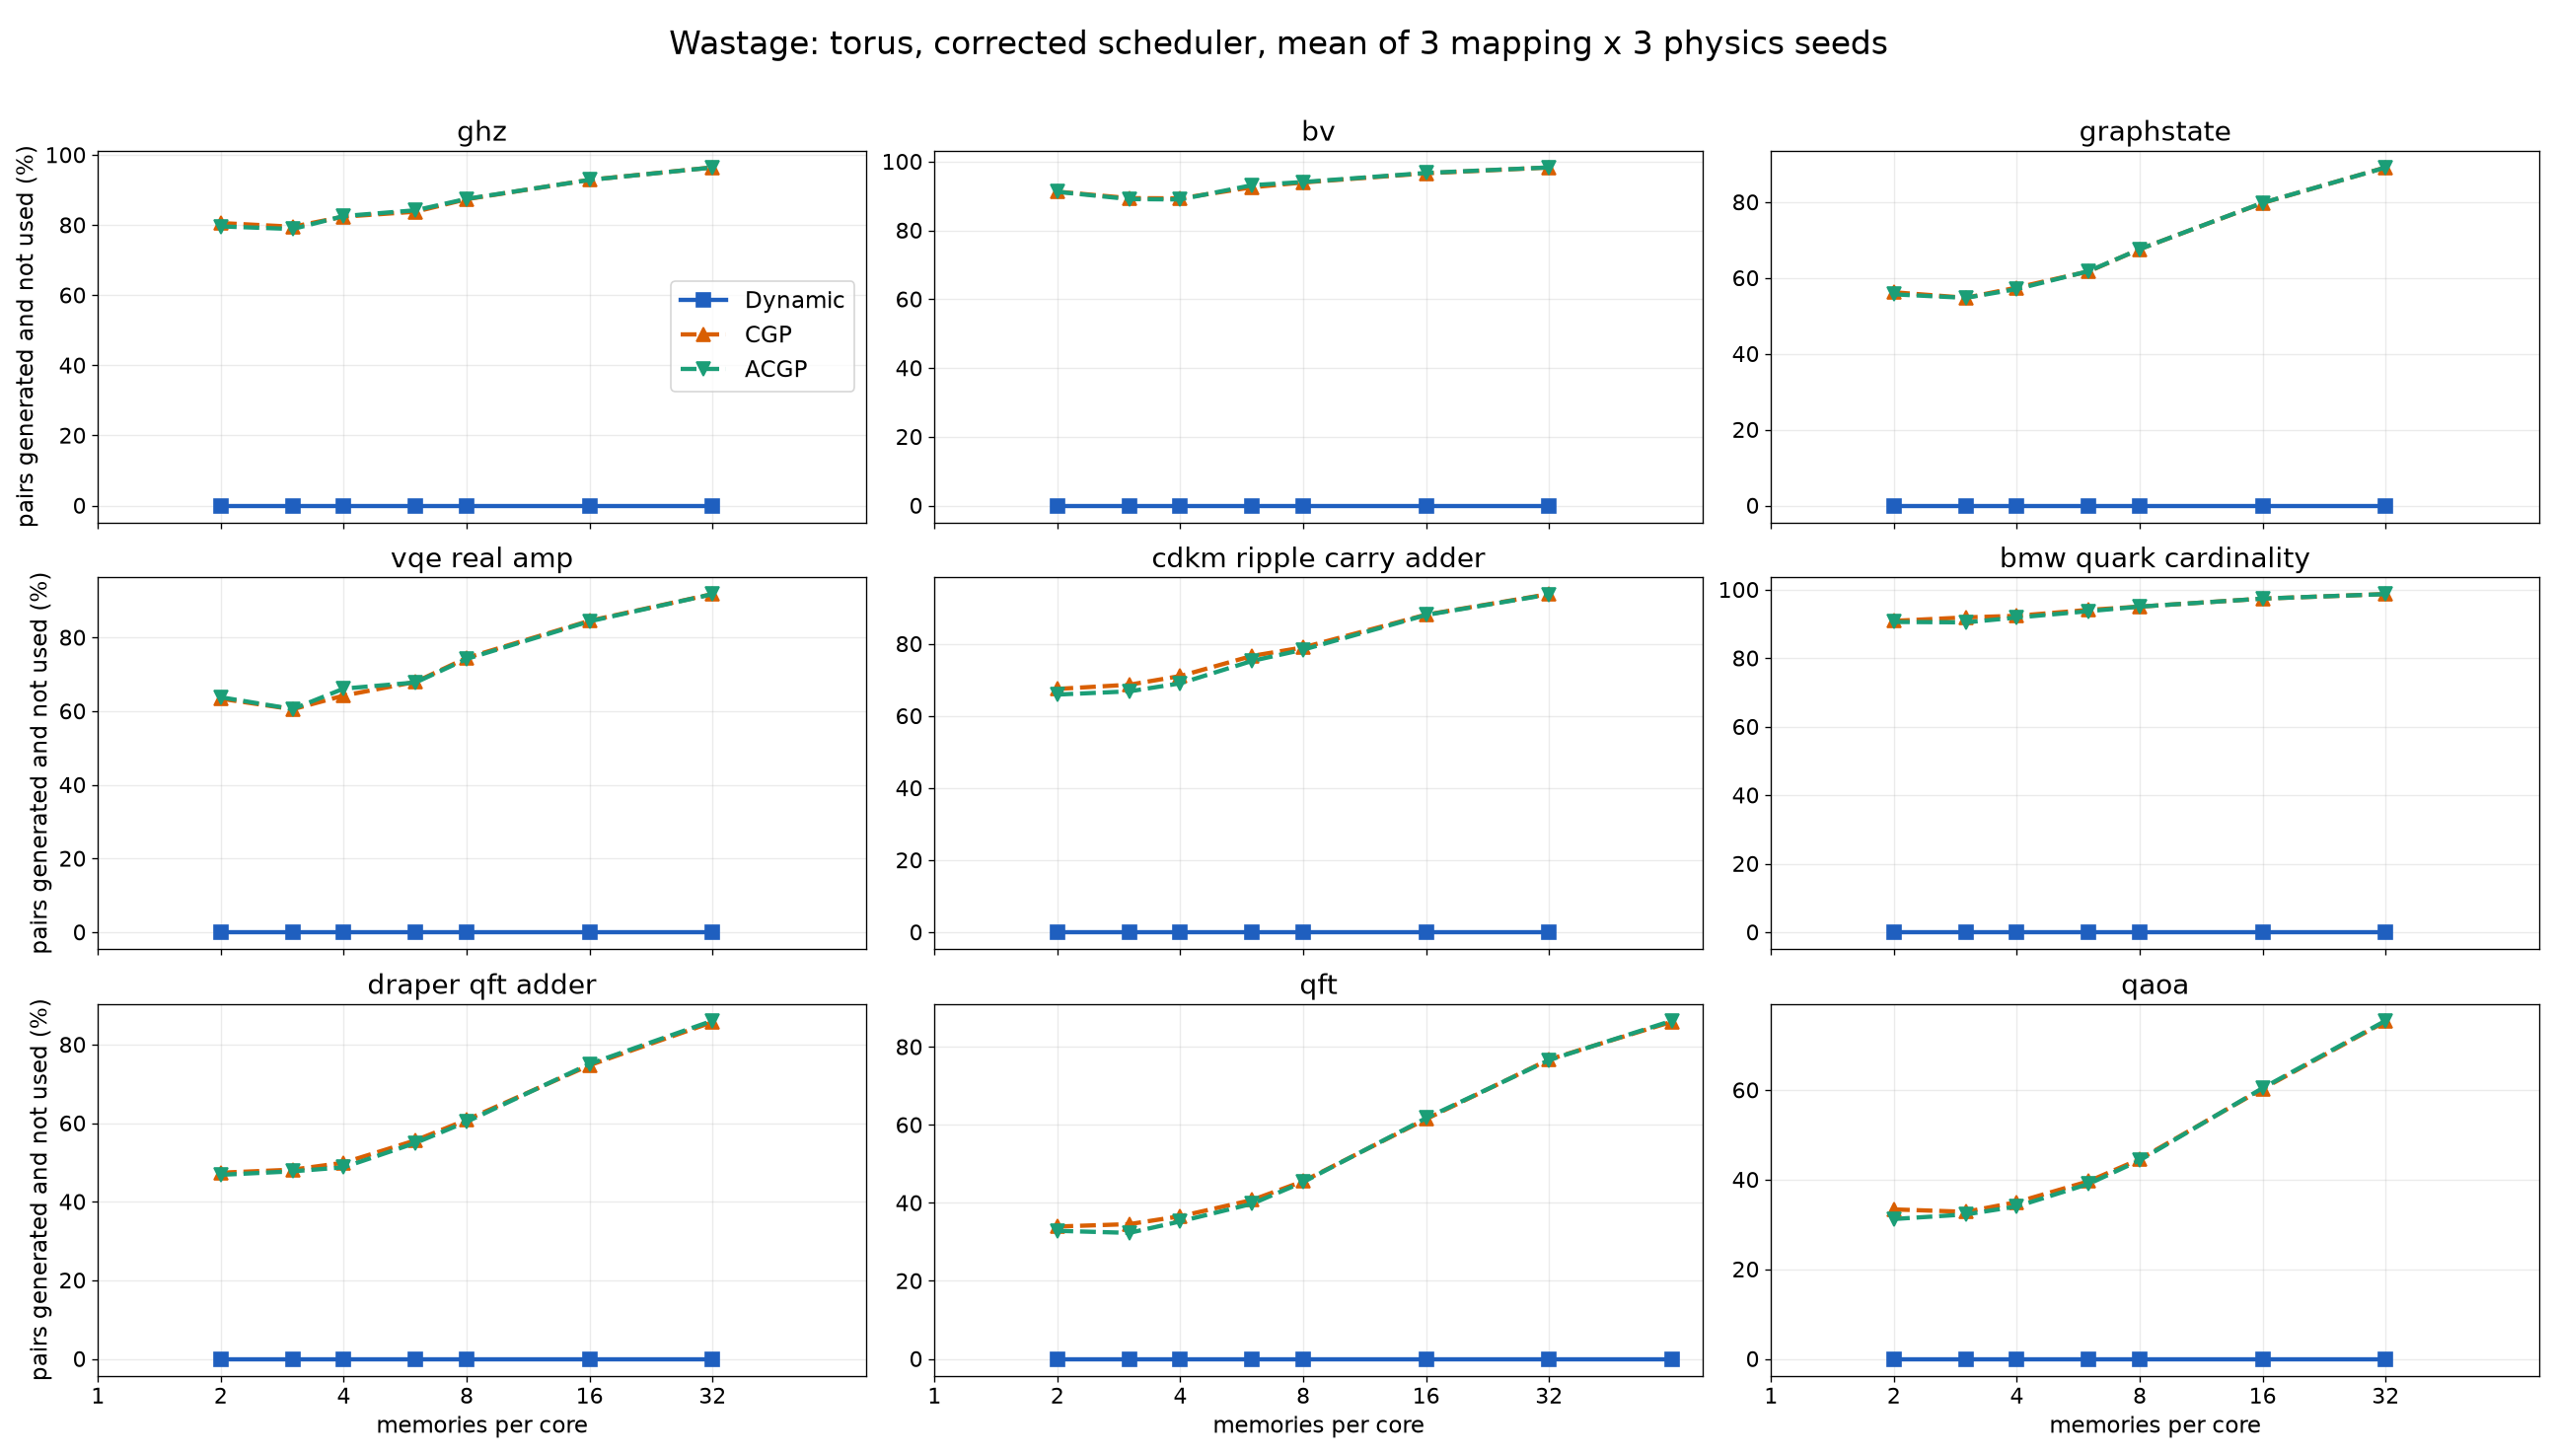
\includegraphics[width=\linewidth,height=0.82\textheight,keepaspectratio]{fp_torus_waste.png}
\caption{Pairs generated and not used by the end of the run, as a percentage of pairs generated (dynamic, CGP, ACGP). Torus, corrected scheduler, mean of three mapping seeds of the mean of three physics seeds; CGP and ACGP cache at most memories$-1$ pairs per core.}
\label{fig:fp-torus-waste}
\end{figure}
\end{landscape}\clearpage\restoregeometry

\clearpage\newgeometry{margin=12mm}\begin{landscape}
\begin{figure}[p]
\centering
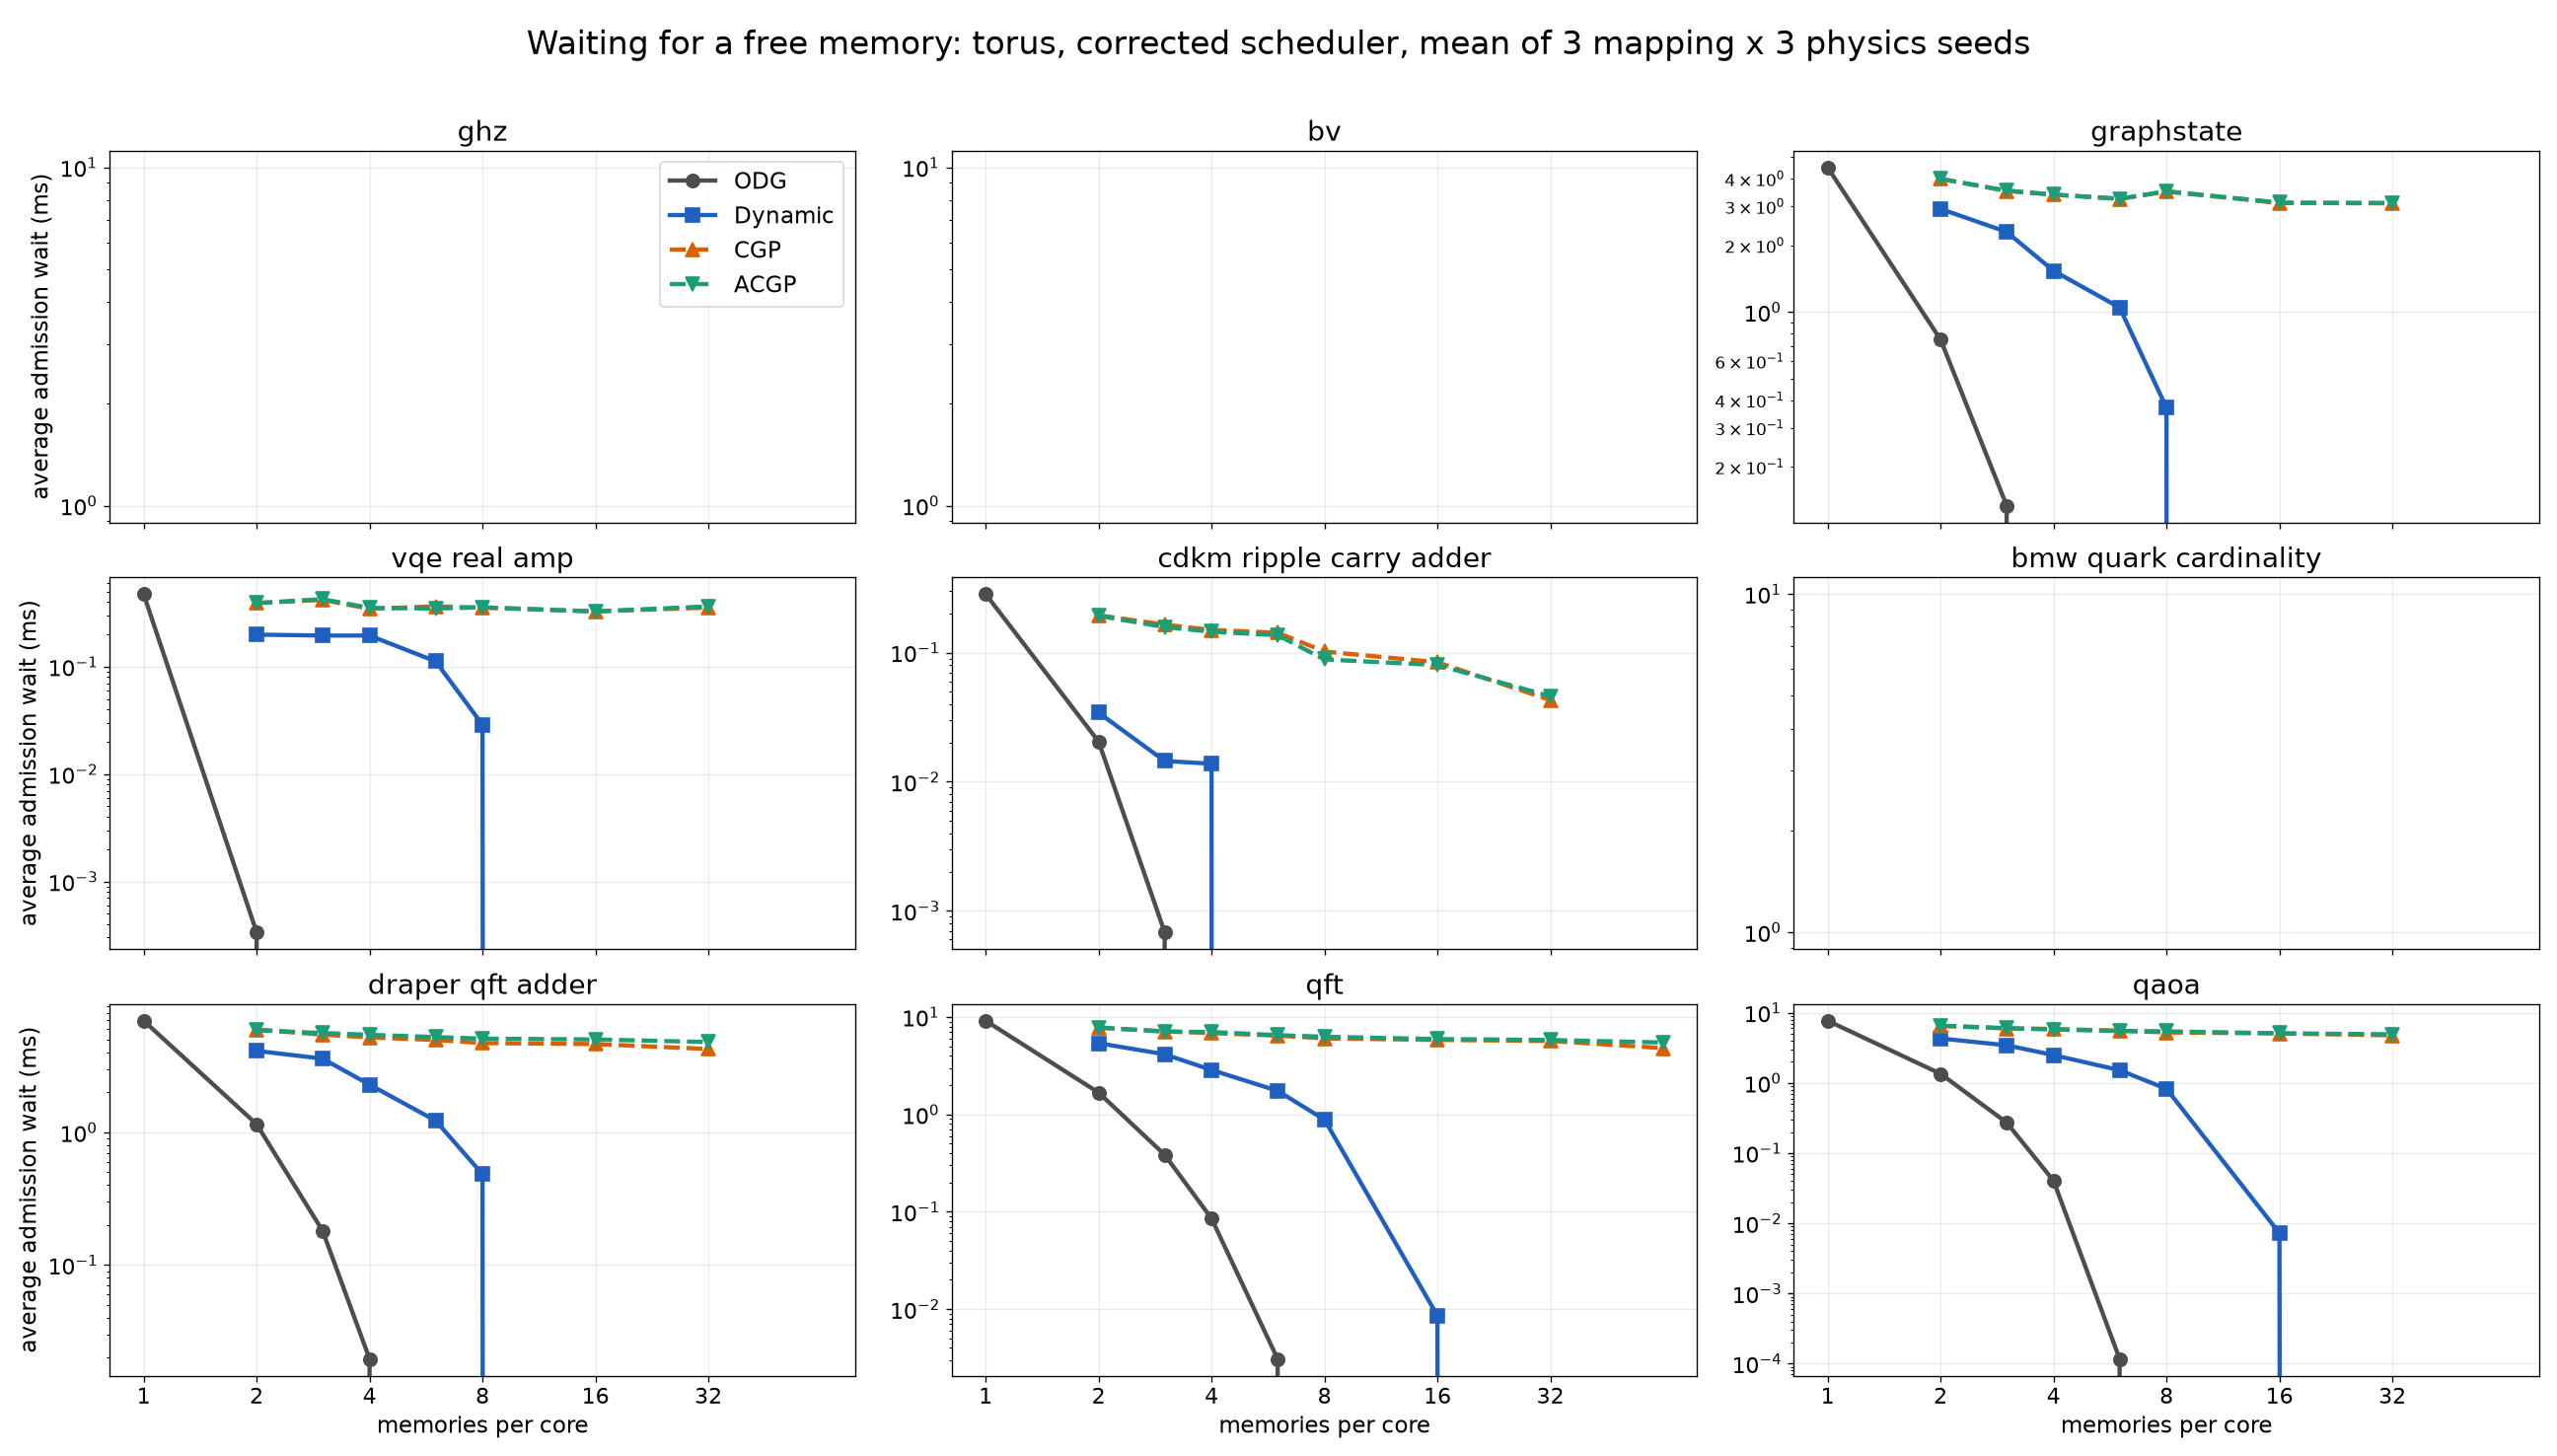
\includegraphics[width=\linewidth,height=0.82\textheight,keepaspectratio]{fp_torus_wait.png}
\caption{Average wait for a free memory (log scale). Torus, corrected scheduler, mean of three mapping seeds of the mean of three physics seeds; CGP and ACGP cache at most memories$-1$ pairs per core.}
\label{fig:fp-torus-wait}
\end{figure}
\end{landscape}\clearpage\restoregeometry

\clearpage\newgeometry{margin=12mm}\begin{landscape}
\begin{figure}[p]
\centering
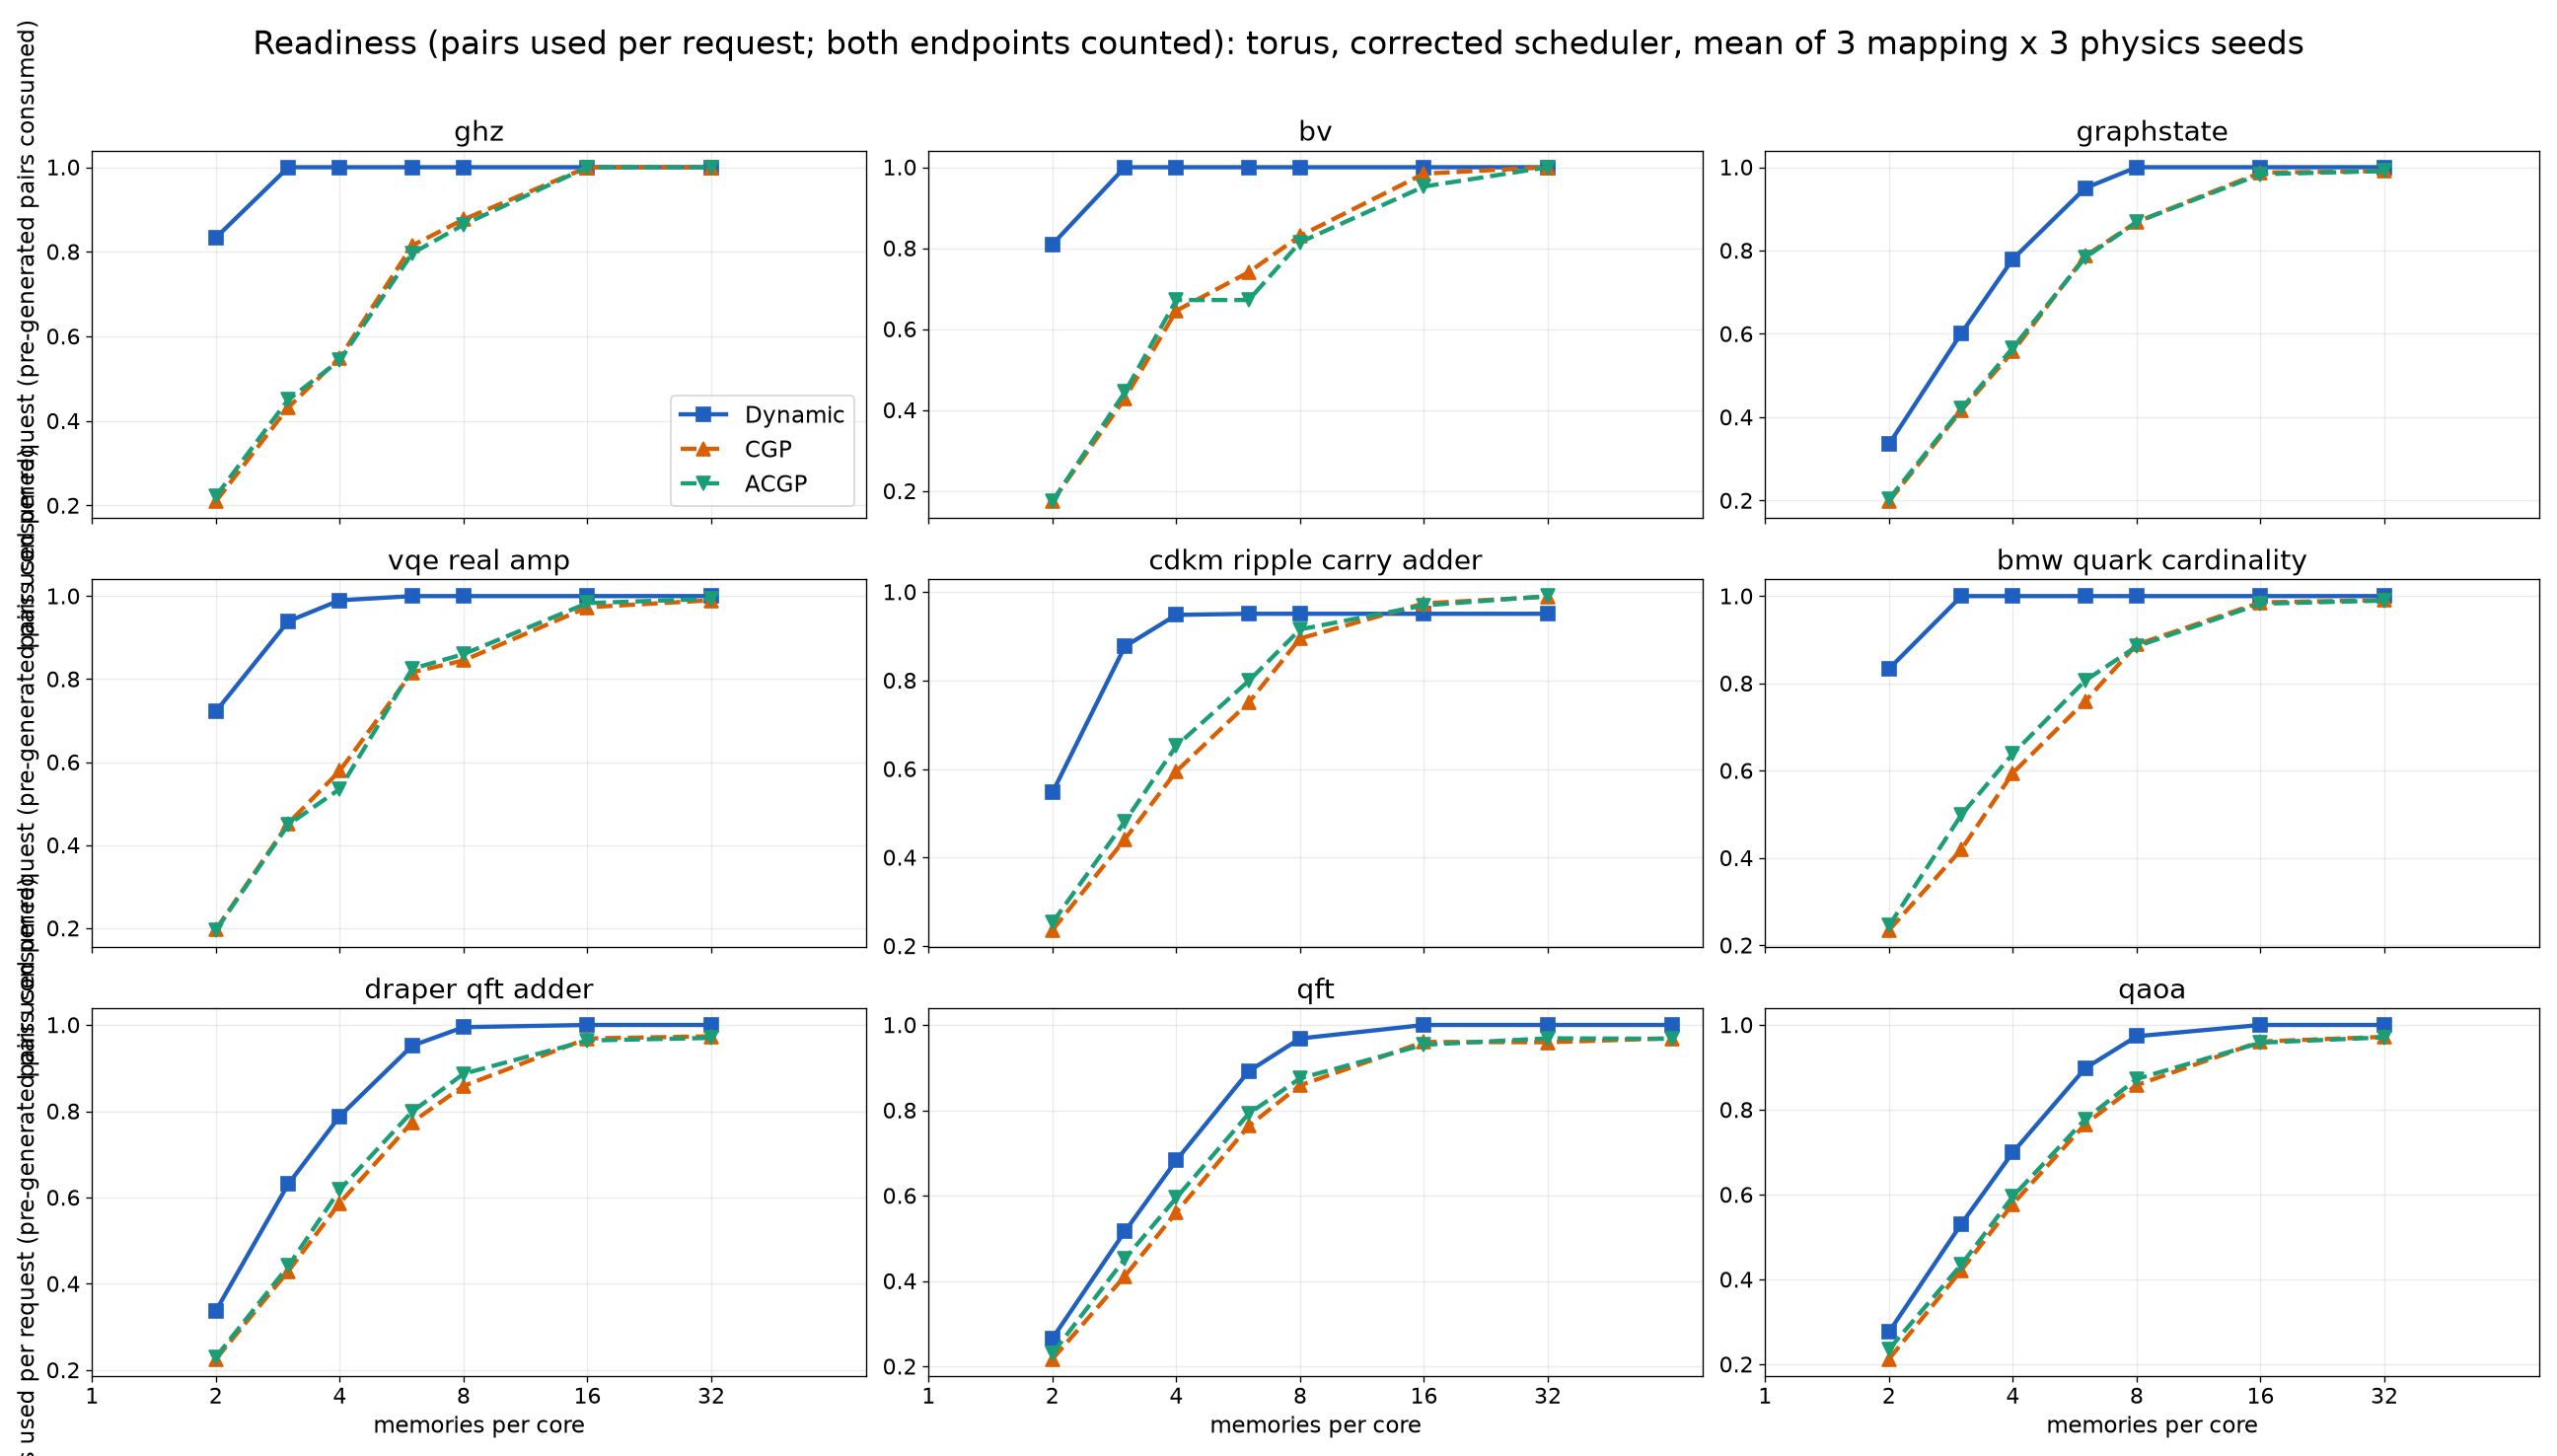
\includegraphics[width=\linewidth,height=0.82\textheight,keepaspectratio]{fp_torus_readiness.png}
\caption{Pre-generated pairs consumed per request (pairs are counted at both endpoints, so the unit is pairs used divided by twice the requests). Torus, corrected scheduler, mean of three mapping seeds of the mean of three physics seeds; CGP and ACGP cache at most memories$-1$ pairs per core.}
\label{fig:fp-torus-ready}
\end{figure}
\end{landscape}\clearpage\restoregeometry


\section{Where dynamic lies}
\begin{itemize}
  \item \textbf{Against the autonomous protocols (the stated goal): yes.} At every modelled memory count (two to four) dynamic has lower latency than CGP and ACGP on every one of the nine benchmarks, wastes none of its pairs against $34$ to $89\%$,
    and delivers higher fidelity on every benchmark ($0.916$ to $0.927$ against $0.865$ to $0.913$ at four memories). This holds on the mesh and on the torus.
  \item \textbf{Against on-demand generation: only partly.} Dynamic matches or beats ODG's latency on the benchmarks where requests rarely compete for memory (five of nine at four memories), and on all of them once the memory count reaches eight to sixteen. On the
    congested benchmarks at the modelled two to four memories it is slower than ODG, by a factor of $2.0$ to $3.5$ on the mesh and $1.8$ to $3.2$ on the torus, because prepared pairs occupy memory that requests need. It never matches ODG's fidelity.
  \item \textbf{What would change this} is not established here. The plan does not account for the memory a ready pair's own request also needs, nor for when a chain hop becomes eligible (Chapter~\ref{ch:why-dynamic}); a planner that did is a possible
    direction, not a result.
\end{itemize}
\paragraph{Limits.} Nine benchmarks (the random circuit was not run for CGP and ACGP); three mapping seeds; ACE's physical parameters, which are undecided (Appendix~\ref{app:params}); the autonomous protocols are configured with a cache cap of memories$-1$, which is my choice for fairness
and is not ACE's default; the waste of the autonomous protocols depends on the length of the workload and is only comparable within a benchmark.

\chapter{Fresh Golden Study: Contract and Execution Record}

This chapter is the living record for the consolidated experiment program. It is
kept separate from historical ACE results so that a result cannot be promoted merely
because it exists in an older output directory. Every accepted observation must have
an immutable trace hash, a configuration manifest, paired seeds, complete requests,
and a source CSV listed in the study registry.

The cross-policy headline metric is request eligibility-to-EPR-delivery latency. It
includes admission wait, reservation, retry, and generation time. It excludes time
before eligibility during which a cached pair was merely stored. Whole-program cost
is reported separately as makespan.

% Generated by tools/golden_study/studyctl.py; do not edit by hand.
\begin{table}[H]
\centering
\caption{Golden-study contract at report build time.}
\begin{tabular}{p{0.30\linewidth}p{0.62\linewidth}}
\toprule
Study identifier & \texttt{golden-ace-2026-10-25} \\
Memory capacities/core & 2, 3, 4, 6, 8, 16, 32, 64 \\
Policies registered & ODG, CGP, ACGP, Dynamic-full-chain, Dynamic-first-hop, Dynamic-congestion-adaptive \\
Torus routing & Dijkstra only \\
\bottomrule
\end{tabular}
\end{table}


The planned capacity study includes constrained settings and deliberately labelled
architecture-scaling settings. Capacities greater than the current four-memory model
are sensitivity points, not claims about the baseline hardware. The torus arm uses
Dijkstra routing only. Mesh routing comparisons hold a placement contract fixed.

At report build time, this chapter contains no performance conclusion until the
contract has been made run-ready and the corresponding registry rows, raw CSV files,
and validation records exist.

\chapter{Limits and open decisions}
\label{ch:limits}

\begin{itemize}
  \item \textbf{Physical parameters are undecided.} ACE's coherence time (1\,s), memory efficiency (0.95) and $2.5$\,cm link differ from the group's multi-core paper (1\,ms, 0.85). Congestion conclusions
        are largely structural; pre-generation and fidelity conclusions depend entirely on them (Chapter~\ref{ch:exp1}).
  \item \textbf{The scheduler is modelled as a central controller} that reads each core's reservation table instantly. A distributed scheduler would see stale tables.
  \item \textbf{Budgets above four are counterfactual.} They say what more memory would buy, not what the hardware has.
  \item \textbf{One machine, one parameter set, nine runs per cell.} Standard deviations pool mapping and physics seeds.
  \item \textbf{Experiment~1 ran on-demand and dynamic;} CGP and ACGP were added in Chapter~\ref{ch:four-policies} for nine benchmarks (the random circuit was set aside for them: its runs at large memory counts take over an hour each). Fixed pre-generation was audited for correctness but not swept.
  \item \textbf{The autonomous protocols' cache cap is my choice.} CGP and ACGP were allowed to hold at most memories$-1$ pairs per core, as dynamic is, instead of ACE's fixed cap of three; their runs end 1\,ms after the last request so that waste covers the workload only. Waste depends on the length of the workload and is comparable only within a benchmark.
  \item \textbf{The diagnosis of Chapter~\ref{ch:why-dynamic} is deep on QFT} (three mapping and three physics seeds at four memories); on the other benchmarks it is one mapping seed.
  \item \textbf{CGP and ACGP pair ages were not measured,} so the lower fidelity of their pairs is not attributed to a measured cause.
  \item \textbf{Harness constants} (5.3\,ms lead, 50\,ms window, 5\,ms empty-layer gap) dominate makespan on short traces and are identical for both schedulers.
  \item \textbf{No routing algorithm is proposed.} Chapter~\ref{ch:routing} bounds what offline routing could achieve structurally and then simulates the optimal offline choice of routes; it does not claim a practical congestion-aware routing algorithm.
  \item Mechanisms marked ``likely'' or ``probably'' in the text were not isolated by an experiment.
\end{itemize}


\appendix
\chapter{Parameters in force}
\label{app:params}

The tables below are generated from the parameter record written by the Experiment~1 driver, which reads the physics from the configuration file and the
other constants from the source, so they cannot drift from what ran.

\begin{table}[H]
\centering\small
\begin{tabular}{@{}lp{0.5\linewidth}@{}}
\toprule
Physical parameter & Value \\
\midrule
Memory fidelity & 0.95 \\
Memory efficiency & 0.95 \\
Memory coherence time & 1 s \\
Memory cut-off ratio (cut-off / coherence) & 1 (SeQUeNCe default; not set in the file) \\
BSM detector efficiencies & 0.95, 0.95 \\
Gate / measurement fidelity & 0.99 / 0.99 \\
Router-to-BSM fibre & 0.025 m, 0.0002 dB/m \\
Classical delay & distance/c + 20 $\mu$s per hop + 100 $\mu$s \\
Configuration file & config/final\_config/grid\_4x4\_ace\_3.json \\
\bottomrule
\end{tabular}
\caption{Physical parameters in force (read from the run's parameter record).}
\label{tab:params-physics}
\end{table}

\begin{table}[H]
\centering\small
\resizebox{\ifdim\width>\linewidth\linewidth\else\width\fi}{!}{%
\begin{tabular}{@{}lp{0.3\linewidth}@{}}
\toprule
Harness constant & Value \\
\midrule
Pre-generation lead (request submitted this long before its window) & 5.3 ms \\
Request reservation window & 50 ms \\
Empty-layer gap & 5 ms \\
Retry period after a physical rejection & 1 ms \\
Admission grace after a release or timeout & 1 ps \\
A ``wait'' means more than & 0.001 ms \\
Compiler reservation window & 1000 ms \\
Planner: delta / lookahead / coherence layers & 6 / 8 / 10 \\
Fidelity threshold of a request & 0.01 \\
Simulation stop time & 300 s \\
Scheduler & per-qubit, admission event, starvation guard on \\
Seeds & mapping [42, 43, 44], physics [0, 1, 2] \\
\bottomrule
\end{tabular}}
\caption{Harness and scheduler constants (not physical).}
\label{tab:params-harness}
\end{table}


\section{Where the physical values come from, and the open decision}
The values were traced to the two neighbouring papers' Table~I. ACE's classical delays, detector efficiency, memory and gate fidelities and fibre attenuation match
the metro-scale adaptive-continuous protocol paper (arXiv 2502.01964), which also gives a $10$\,km link, a $2$\,s coherence time and a memory efficiency of $0.6$.
ACE's link is $0.025$ (read as metres), its coherence time $1$\,s and its memory efficiency $0.95$. The group's multi-core paper (arXiv 2607.14592) states coherence $1$\,ms
and memory efficiency $0.85$. The sensitivity arm of Experiment~1 shows that this choice decides every pre-generation and fidelity conclusion; it is the most important open
decision, and the question for the supervisor is written in \code{docs/reports/ace-physical-parameters.md}.

\chapter{Reproducing the results}
\label{app:repro}

All commands are run from the repository root with the project's Python environment. Result folders are dated 2026-10-24.
\begin{itemize}
  \item Legacy baseline: \code{python tools/ace_correctness/baseline.py check --golden results/ace_correctness_baseline_2026-10-24/legacy --strict}
  \item Unit and microcase tests: \code{python -B -m unittest discover -s test -p 'test_*.py'}
  \item Heatmap: \code{python tools/heatmap/regenerate_heatmap.py --output out}
  \item Experiment~2: \code{python tools/experiment2/make_report.py}
  \item Experiment~1: \code{python tools/experiment1/run_experiment1.py --output out --jobs 4}, then \code{python tools/experiment1/analyze.py --results out/results.csv --output out}
  \item Offline routing: \code{python tools/routing_research/run_routing_study.py --output out}
  \item Torus traces: \code{python tools/congestion_study/run_study.py --mapper-dir mapper --topology torus --mapping-only --seeds 42 43 44 ...}
  \item Torus experiments: \code{sh tools/torus/run_torus_experiments.sh WORKDIR}
  \item This report's tables: \code{python tools/latex/make_tables.py}, then \code{tectonic docs/latex/ace_report/main.tex}
\end{itemize}
Every experiment folder contains \code{run_parameters.json} (all parameters, trace hashes, code commit, machine) and, where timed, \code{timings.csv}.

\chapter{Experiment 1: every cell}
\label{app:full}
All workloads, both policies and every budget, with the nine runs behind each cell summarised. The same data are in \code{results/experiment1_ten_benchmarks_2026-10-24/results.csv} (one row per run) and \code{cell_summary.csv}.
{\scriptsize\setlength{\tabcolsep}{2.4pt}
\begin{longtable}{@{}llrrrrrrrr@{}}
\caption{Experiment 1, every cell: nine runs (three mapping $\times$ three physics seeds). Latency in ms (mean, standard deviation, minimum--maximum); makespan in seconds; Waited is the fraction of requests that waited more than a microsecond; Retries the mean number of physical rejections per run. $^*$ counterfactual budget.}\label{tab:exp1-full}\\
\toprule
Workload & Policy & Mem. & Latency ms & sd & min--max & Fidelity & Makespan s & Waited & Retries \\
\midrule
\endfirsthead
\toprule
Workload & Policy & Mem. & Latency ms & sd & min--max & Fidelity & Makespan s & Waited & Retries \\
\midrule
\endhead
\bottomrule
\endfoot
GHZ & on-demand & 1 & 1.171 & 0.112 & 1.029--1.342 & 0.9498 & 0.33 & 0.000 & 0.00 \\
GHZ & on-demand & 2 & 1.171 & 0.112 & 1.029--1.342 & 0.9498 & 0.33 & 0.000 & 0.00 \\
GHZ & on-demand & 3 & 1.171 & 0.112 & 1.029--1.342 & 0.9498 & 0.33 & 0.000 & 0.00 \\
GHZ & on-demand & 4 & 1.171 & 0.112 & 1.029--1.342 & 0.9498 & 0.33 & 0.000 & 0.00 \\
GHZ & on-demand & 6$^*$ & 1.171 & 0.112 & 1.029--1.342 & 0.9498 & 0.33 & 0.000 & 0.00 \\
GHZ & on-demand & 8$^*$ & 1.171 & 0.112 & 1.029--1.342 & 0.9498 & 0.33 & 0.000 & 0.00 \\
GHZ & on-demand & 16$^*$ & 1.171 & 0.112 & 1.029--1.342 & 0.9498 & 0.33 & 0.000 & 0.00 \\
GHZ & on-demand & 32$^*$ & 1.171 & 0.112 & 1.029--1.342 & 0.9498 & 0.33 & 0.000 & 0.00 \\
GHZ & dynamic & 2 & 0.512 & 0.066 & 0.396--0.600 & 0.9344 & 0.31 & 0.000 & 0.00 \\
GHZ & dynamic & 3 & 0.263 & 0.000 & 0.263--0.263 & 0.9254 & 0.30 & 0.000 & 0.00 \\
GHZ & dynamic & 4 & 0.263 & 0.000 & 0.263--0.263 & 0.9254 & 0.30 & 0.000 & 0.00 \\
GHZ & dynamic & 6$^*$ & 0.263 & 0.000 & 0.263--0.263 & 0.9254 & 0.30 & 0.000 & 0.00 \\
GHZ & dynamic & 8$^*$ & 0.263 & 0.000 & 0.263--0.263 & 0.9254 & 0.30 & 0.000 & 0.00 \\
GHZ & dynamic & 16$^*$ & 0.263 & 0.000 & 0.263--0.263 & 0.9254 & 0.30 & 0.000 & 0.00 \\
GHZ & dynamic & 32$^*$ & 0.263 & 0.000 & 0.263--0.263 & 0.9254 & 0.30 & 0.000 & 0.00 \\
Bernstein--Vazirani & on-demand & 1 & 1.221 & 0.115 & 1.120--1.404 & 0.9498 & 0.89 & 0.000 & 0.00 \\
Bernstein--Vazirani & on-demand & 2 & 1.221 & 0.115 & 1.120--1.404 & 0.9498 & 0.89 & 0.000 & 0.00 \\
Bernstein--Vazirani & on-demand & 3 & 1.221 & 0.115 & 1.120--1.404 & 0.9498 & 0.89 & 0.000 & 0.00 \\
Bernstein--Vazirani & on-demand & 4 & 1.221 & 0.115 & 1.120--1.404 & 0.9498 & 0.89 & 0.000 & 0.00 \\
Bernstein--Vazirani & on-demand & 6$^*$ & 1.221 & 0.115 & 1.120--1.404 & 0.9498 & 0.89 & 0.000 & 0.00 \\
Bernstein--Vazirani & on-demand & 8$^*$ & 1.221 & 0.115 & 1.120--1.404 & 0.9498 & 0.89 & 0.000 & 0.00 \\
Bernstein--Vazirani & on-demand & 16$^*$ & 1.221 & 0.115 & 1.120--1.404 & 0.9498 & 0.89 & 0.000 & 0.00 \\
Bernstein--Vazirani & on-demand & 32$^*$ & 1.221 & 0.115 & 1.120--1.404 & 0.9498 & 0.89 & 0.000 & 0.00 \\
Bernstein--Vazirani & dynamic & 2 & 0.464 & 0.067 & 0.372--0.584 & 0.9345 & 0.87 & 0.000 & 0.00 \\
Bernstein--Vazirani & dynamic & 3 & 0.244 & 0.000 & 0.244--0.244 & 0.9266 & 0.86 & 0.000 & 0.00 \\
Bernstein--Vazirani & dynamic & 4 & 0.244 & 0.000 & 0.244--0.244 & 0.9266 & 0.86 & 0.000 & 0.00 \\
Bernstein--Vazirani & dynamic & 6$^*$ & 0.244 & 0.000 & 0.244--0.244 & 0.9266 & 0.86 & 0.000 & 0.00 \\
Bernstein--Vazirani & dynamic & 8$^*$ & 0.244 & 0.000 & 0.244--0.244 & 0.9266 & 0.86 & 0.000 & 0.00 \\
Bernstein--Vazirani & dynamic & 16$^*$ & 0.244 & 0.000 & 0.244--0.244 & 0.9266 & 0.86 & 0.000 & 0.00 \\
Bernstein--Vazirani & dynamic & 32$^*$ & 0.244 & 0.000 & 0.244--0.244 & 0.9266 & 0.86 & 0.000 & 0.00 \\
BMW/QUARK cardinality & on-demand & 1 & 1.120 & 0.041 & 1.056--1.183 & 0.9498 & 6.95 & 0.000 & 0.00 \\
BMW/QUARK cardinality & on-demand & 2 & 1.120 & 0.041 & 1.056--1.183 & 0.9498 & 6.95 & 0.000 & 0.00 \\
BMW/QUARK cardinality & on-demand & 3 & 1.120 & 0.041 & 1.056--1.183 & 0.9498 & 6.95 & 0.000 & 0.00 \\
BMW/QUARK cardinality & on-demand & 4 & 1.120 & 0.041 & 1.056--1.183 & 0.9498 & 6.95 & 0.000 & 0.00 \\
BMW/QUARK cardinality & on-demand & 6$^*$ & 1.120 & 0.041 & 1.056--1.183 & 0.9498 & 6.95 & 0.000 & 0.00 \\
BMW/QUARK cardinality & on-demand & 8$^*$ & 1.120 & 0.041 & 1.056--1.183 & 0.9498 & 6.95 & 0.000 & 0.00 \\
BMW/QUARK cardinality & on-demand & 16$^*$ & 1.120 & 0.041 & 1.056--1.183 & 0.9498 & 6.95 & 0.000 & 0.00 \\
BMW/QUARK cardinality & on-demand & 32$^*$ & 1.120 & 0.041 & 1.056--1.183 & 0.9498 & 6.95 & 0.000 & 0.00 \\
BMW/QUARK cardinality & dynamic & 2 & 0.488 & 0.016 & 0.458--0.510 & 0.9343 & 6.86 & 0.000 & 0.00 \\
BMW/QUARK cardinality & dynamic & 3 & 0.250 & 0.000 & 0.250--0.250 & 0.9253 & 6.83 & 0.000 & 0.00 \\
BMW/QUARK cardinality & dynamic & 4 & 0.250 & 0.000 & 0.250--0.250 & 0.9253 & 6.83 & 0.000 & 0.00 \\
BMW/QUARK cardinality & dynamic & 6$^*$ & 0.250 & 0.000 & 0.250--0.250 & 0.9253 & 6.83 & 0.000 & 0.00 \\
BMW/QUARK cardinality & dynamic & 8$^*$ & 0.250 & 0.000 & 0.250--0.250 & 0.9253 & 6.83 & 0.000 & 0.00 \\
BMW/QUARK cardinality & dynamic & 16$^*$ & 0.250 & 0.000 & 0.250--0.250 & 0.9253 & 6.83 & 0.000 & 0.00 \\
BMW/QUARK cardinality & dynamic & 32$^*$ & 0.250 & 0.000 & 0.250--0.250 & 0.9253 & 6.83 & 0.000 & 0.00 \\
VQE real amplitudes & on-demand & 1 & 2.324 & 0.139 & 2.121--2.568 & 0.9498 & 0.74 & 0.205 & 0.00 \\
VQE real amplitudes & on-demand & 2 & 1.112 & 0.047 & 1.043--1.175 & 0.9498 & 0.68 & 0.002 & 0.00 \\
VQE real amplitudes & on-demand & 3 & 1.112 & 0.047 & 1.043--1.174 & 0.9498 & 0.68 & 0.000 & 0.00 \\
VQE real amplitudes & on-demand & 4 & 1.112 & 0.047 & 1.043--1.174 & 0.9498 & 0.68 & 0.000 & 0.00 \\
VQE real amplitudes & on-demand & 6$^*$ & 1.112 & 0.047 & 1.043--1.174 & 0.9498 & 0.68 & 0.000 & 0.00 \\
VQE real amplitudes & on-demand & 8$^*$ & 1.112 & 0.047 & 1.043--1.174 & 0.9498 & 0.68 & 0.000 & 0.00 \\
VQE real amplitudes & on-demand & 16$^*$ & 1.112 & 0.047 & 1.043--1.174 & 0.9498 & 0.68 & 0.000 & 0.00 \\
VQE real amplitudes & on-demand & 32$^*$ & 1.112 & 0.047 & 1.043--1.174 & 0.9498 & 0.68 & 0.000 & 0.00 \\
VQE real amplitudes & dynamic & 2 & 1.524 & 0.205 & 1.251--1.829 & 0.9344 & 0.68 & 0.184 & 0.00 \\
VQE real amplitudes & dynamic & 3 & 1.195 & 0.161 & 0.954--1.433 & 0.9203 & 0.65 & 0.176 & 0.00 \\
VQE real amplitudes & dynamic & 4 & 0.878 & 0.072 & 0.821--0.994 & 0.9165 & 0.63 & 0.141 & 0.00 \\
VQE real amplitudes & dynamic & 6$^*$ & 0.413 & 0.000 & 0.413--0.413 & 0.9128 & 0.62 & 0.032 & 0.00 \\
VQE real amplitudes & dynamic & 8$^*$ & 0.253 & 0.000 & 0.253--0.253 & 0.9125 & 0.61 & 0.000 & 0.00 \\
VQE real amplitudes & dynamic & 16$^*$ & 0.253 & 0.000 & 0.253--0.253 & 0.9125 & 0.61 & 0.000 & 0.00 \\
VQE real amplitudes & dynamic & 32$^*$ & 0.253 & 0.000 & 0.253--0.253 & 0.9125 & 0.61 & 0.000 & 0.00 \\
CDKM ripple-carry adder & on-demand & 1 & 1.658 & 0.221 & 1.362--1.979 & 0.9498 & 5.62 & 0.033 & 0.00 \\
CDKM ripple-carry adder & on-demand & 2 & 1.242 & 0.054 & 1.160--1.311 & 0.9498 & 5.59 & 0.020 & 0.00 \\
CDKM ripple-carry adder & on-demand & 3 & 1.165 & 0.033 & 1.119--1.215 & 0.9498 & 5.58 & 0.011 & 0.00 \\
CDKM ripple-carry adder & on-demand & 4 & 1.138 & 0.027 & 1.100--1.178 & 0.9498 & 5.58 & 0.002 & 0.00 \\
CDKM ripple-carry adder & on-demand & 6$^*$ & 1.137 & 0.027 & 1.099--1.178 & 0.9498 & 5.58 & 0.000 & 0.00 \\
CDKM ripple-carry adder & on-demand & 8$^*$ & 1.137 & 0.027 & 1.099--1.178 & 0.9498 & 5.58 & 0.000 & 0.00 \\
CDKM ripple-carry adder & on-demand & 16$^*$ & 1.137 & 0.027 & 1.099--1.178 & 0.9498 & 5.58 & 0.000 & 0.00 \\
CDKM ripple-carry adder & on-demand & 32$^*$ & 1.137 & 0.027 & 1.099--1.178 & 0.9498 & 5.58 & 0.000 & 0.00 \\
CDKM ripple-carry adder & dynamic & 2 & 0.764 & 0.059 & 0.656--0.838 & 0.9354 & 5.37 & 0.021 & 0.00 \\
CDKM ripple-carry adder & dynamic & 3 & 0.380 & 0.027 & 0.350--0.417 & 0.9247 & 5.22 & 0.014 & 0.00 \\
CDKM ripple-carry adder & dynamic & 4 & 0.303 & 0.008 & 0.293--0.315 & 0.9227 & 5.20 & 0.003 & 0.00 \\
CDKM ripple-carry adder & dynamic & 6$^*$ & 0.298 & 0.006 & 0.292--0.307 & 0.9210 & 5.20 & 0.000 & 0.00 \\
CDKM ripple-carry adder & dynamic & 8$^*$ & 0.298 & 0.006 & 0.292--0.307 & 0.9210 & 5.20 & 0.000 & 0.00 \\
CDKM ripple-carry adder & dynamic & 16$^*$ & 0.298 & 0.006 & 0.292--0.307 & 0.9210 & 5.20 & 0.000 & 0.00 \\
CDKM ripple-carry adder & dynamic & 32$^*$ & 0.298 & 0.006 & 0.292--0.307 & 0.9210 & 5.20 & 0.000 & 0.00 \\
Graph state & on-demand & 1 & 9.138 & 1.141 & 7.970--10.778 & 0.9498 & 0.38 & 0.602 & 0.00 \\
Graph state & on-demand & 2 & 2.722 & 0.541 & 2.268--3.708 & 0.9498 & 0.26 & 0.281 & 0.00 \\
Graph state & on-demand & 3 & 1.528 & 0.304 & 1.197--2.051 & 0.9498 & 0.24 & 0.121 & 0.00 \\
Graph state & on-demand & 4 & 1.239 & 0.131 & 1.053--1.472 & 0.9498 & 0.24 & 0.029 & 0.00 \\
Graph state & on-demand & 6$^*$ & 1.177 & 0.080 & 1.040--1.278 & 0.9498 & 0.24 & 0.000 & 0.00 \\
Graph state & on-demand & 8$^*$ & 1.177 & 0.080 & 1.040--1.278 & 0.9498 & 0.24 & 0.000 & 0.00 \\
Graph state & on-demand & 16$^*$ & 1.177 & 0.080 & 1.040--1.278 & 0.9498 & 0.24 & 0.000 & 0.00 \\
Graph state & on-demand & 32$^*$ & 1.177 & 0.080 & 1.040--1.278 & 0.9498 & 0.24 & 0.000 & 0.00 \\
Graph state & dynamic & 2 & 6.360 & 0.793 & 5.193--7.251 & 0.9341 & 0.32 & 0.488 & 0.00 \\
Graph state & dynamic & 3 & 5.011 & 0.592 & 4.329--5.909 & 0.9236 & 0.30 & 0.444 & 0.00 \\
Graph state & dynamic & 4 & 3.234 & 0.817 & 2.336--4.361 & 0.9189 & 0.26 & 0.374 & 0.00 \\
Graph state & dynamic & 6$^*$ & 1.603 & 0.389 & 1.324--2.272 & 0.9158 & 0.24 & 0.224 & 0.00 \\
Graph state & dynamic & 8$^*$ & 0.951 & 0.131 & 0.783--1.125 & 0.9128 & 0.23 & 0.173 & 0.00 \\
Graph state & dynamic & 16$^*$ & 0.274 & 0.036 & 0.250--0.322 & 0.9111 & 0.22 & 0.004 & 0.00 \\
Graph state & dynamic & 32$^*$ & 0.250 & 0.000 & 0.250--0.250 & 0.9112 & 0.22 & 0.000 & 0.00 \\
Draper QFT adder & on-demand & 1 & 7.355 & 0.840 & 6.208--8.013 & 0.9498 & 6.89 & 0.536 & 0.00 \\
Draper QFT adder & on-demand & 2 & 2.157 & 0.204 & 1.863--2.329 & 0.9498 & 5.14 & 0.211 & 0.00 \\
Draper QFT adder & on-demand & 3 & 1.298 & 0.053 & 1.213--1.357 & 0.9498 & 4.90 & 0.055 & 0.00 \\
Draper QFT adder & on-demand & 4 & 1.150 & 0.022 & 1.126--1.188 & 0.9498 & 4.88 & 0.008 & 0.00 \\
Draper QFT adder & on-demand & 6$^*$ & 1.134 & 0.020 & 1.108--1.165 & 0.9498 & 4.87 & 0.000 & 0.00 \\
Draper QFT adder & on-demand & 8$^*$ & 1.134 & 0.020 & 1.108--1.165 & 0.9498 & 4.87 & 0.000 & 0.00 \\
Draper QFT adder & on-demand & 16$^*$ & 1.134 & 0.020 & 1.108--1.165 & 0.9498 & 4.87 & 0.000 & 0.00 \\
Draper QFT adder & on-demand & 32$^*$ & 1.134 & 0.020 & 1.108--1.165 & 0.9498 & 4.87 & 0.000 & 0.00 \\
Draper QFT adder & dynamic & 2 & 4.546 & 0.426 & 3.947--4.915 & 0.9368 & 5.91 & 0.459 & 0.33 \\
Draper QFT adder & dynamic & 3 & 3.666 & 0.341 & 3.195--4.017 & 0.9257 & 5.46 & 0.417 & 1.22 \\
Draper QFT adder & dynamic & 4 & 2.481 & 0.376 & 2.062--2.947 & 0.9218 & 5.03 & 0.317 & 2.44 \\
Draper QFT adder & dynamic & 6$^*$ & 1.599 & 0.169 & 1.375--1.746 & 0.9154 & 4.75 & 0.227 & 2.78 \\
Draper QFT adder & dynamic & 8$^*$ & 0.893 & 0.228 & 0.593--1.088 & 0.9148 & 4.54 & 0.118 & 4.44 \\
Draper QFT adder & dynamic & 16$^*$ & 0.254 & 0.006 & 0.250--0.263 & 0.9158 & 4.41 & 0.000 & 1.00 \\
Draper QFT adder & dynamic & 32$^*$ & 0.250 & 0.000 & 0.250--0.250 & 0.9158 & 4.41 & 0.000 & 0.00 \\
QAOA & on-demand & 1 & 10.925 & 0.405 & 10.452--11.462 & 0.9498 & 10.69 & 0.671 & 0.00 \\
QAOA & on-demand & 2 & 3.421 & 0.140 & 3.248--3.620 & 0.9498 & 6.60 & 0.376 & 0.00 \\
QAOA & on-demand & 3 & 1.740 & 0.057 & 1.665--1.818 & 0.9498 & 5.71 & 0.172 & 0.00 \\
QAOA & on-demand & 4 & 1.273 & 0.022 & 1.231--1.299 & 0.9498 & 5.48 & 0.058 & 0.00 \\
QAOA & on-demand & 6$^*$ & 1.141 & 0.011 & 1.127--1.159 & 0.9498 & 5.41 & 0.004 & 0.00 \\
QAOA & on-demand & 8$^*$ & 1.134 & 0.011 & 1.118--1.149 & 0.9498 & 5.40 & 0.000 & 0.00 \\
QAOA & on-demand & 16$^*$ & 1.134 & 0.011 & 1.119--1.149 & 0.9498 & 5.40 & 0.000 & 0.00 \\
QAOA & on-demand & 32$^*$ & 1.134 & 0.011 & 1.119--1.149 & 0.9498 & 5.40 & 0.000 & 0.00 \\
QAOA & dynamic & 2 & 6.887 & 0.280 & 6.584--7.252 & 0.9390 & 8.50 & 0.576 & 1.00 \\
QAOA & dynamic & 3 & 5.334 & 0.191 & 5.147--5.657 & 0.9298 & 7.43 & 0.519 & 5.67 \\
QAOA & dynamic & 4 & 3.879 & 0.165 & 3.659--4.088 & 0.9245 & 6.62 & 0.454 & 5.67 \\
QAOA & dynamic & 6$^*$ & 2.705 & 0.132 & 2.587--2.900 & 0.9167 & 5.98 & 0.353 & 9.33 \\
QAOA & dynamic & 8$^*$ & 1.857 & 0.085 & 1.787--1.974 & 0.9136 & 5.52 & 0.262 & 10.89 \\
QAOA & dynamic & 16$^*$ & 0.355 & 0.036 & 0.307--0.380 & 0.9137 & 4.78 & 0.020 & 11.89 \\
QAOA & dynamic & 32$^*$ & 0.250 & 0.000 & 0.250--0.250 & 0.9143 & 4.74 & 0.000 & 0.00 \\
QFT & on-demand & 1 & 14.417 & 0.352 & 13.954--14.870 & 0.9498 & 9.11 & 0.696 & 0.00 \\
QFT & on-demand & 2 & 4.721 & 0.145 & 4.572--4.936 & 0.9498 & 5.72 & 0.430 & 0.00 \\
QFT & on-demand & 3 & 2.386 & 0.085 & 2.267--2.506 & 0.9498 & 4.91 & 0.249 & 0.00 \\
QFT & on-demand & 4 & 1.589 & 0.046 & 1.548--1.665 & 0.9498 & 4.66 & 0.130 & 0.00 \\
QFT & on-demand & 6$^*$ & 1.205 & 0.017 & 1.185--1.228 & 0.9498 & 4.53 & 0.031 & 0.00 \\
QFT & on-demand & 8$^*$ & 1.148 & 0.017 & 1.124--1.171 & 0.9498 & 4.51 & 0.007 & 0.00 \\
QFT & on-demand & 16$^*$ & 1.135 & 0.015 & 1.113--1.160 & 0.9498 & 4.51 & 0.000 & 0.00 \\
QFT & on-demand & 32$^*$ & 1.135 & 0.015 & 1.113--1.160 & 0.9498 & 4.51 & 0.000 & 0.00 \\
QFT & on-demand & 64$^*$ & 1.135 & 0.015 & 1.113--1.160 & 0.9498 & 4.51 & 0.000 & 0.00 \\
QFT & dynamic & 2 & 10.056 & 0.537 & 9.410--10.752 & 0.9386 & 7.50 & 0.636 & 0.44 \\
QFT & dynamic & 3 & 7.489 & 0.330 & 7.002--7.730 & 0.9306 & 6.50 & 0.593 & 1.33 \\
QFT & dynamic & 4 & 5.566 & 0.214 & 5.347--5.921 & 0.9274 & 5.75 & 0.513 & 0.89 \\
QFT & dynamic & 6$^*$ & 3.726 & 0.246 & 3.425--4.015 & 0.9215 & 5.12 & 0.414 & 0.56 \\
QFT & dynamic & 8$^*$ & 2.783 & 0.190 & 2.613--3.061 & 0.9189 & 4.79 & 0.328 & 0.44 \\
QFT & dynamic & 16$^*$ & 0.803 & 0.156 & 0.683--1.011 & 0.9185 & 4.19 & 0.082 & 0.00 \\
QFT & dynamic & 32$^*$ & 0.250 & 0.000 & 0.250--0.250 & 0.9202 & 4.05 & 0.000 & 0.00 \\
QFT & dynamic & 64$^*$ & 0.250 & 0.000 & 0.250--0.250 & 0.9202 & 4.05 & 0.000 & 0.00 \\
Random circuit & on-demand & 1 & 2.989 & 0.104 & 2.889--3.134 & 0.9498 & 59.78 & 0.254 & 0.00 \\
Random circuit & on-demand & 2 & 1.265 & 0.019 & 1.238--1.294 & 0.9498 & 51.50 & 0.042 & 0.00 \\
Random circuit & on-demand & 3 & 1.123 & 0.007 & 1.115--1.134 & 0.9498 & 50.93 & 0.006 & 0.00 \\
Random circuit & on-demand & 4 & 1.110 & 0.007 & 1.103--1.122 & 0.9498 & 50.89 & 0.001 & 0.00 \\
Random circuit & on-demand & 6$^*$ & 1.109 & 0.006 & 1.101--1.120 & 0.9498 & 50.89 & 0.000 & 0.00 \\
Random circuit & on-demand & 8$^*$ & 1.109 & 0.006 & 1.101--1.120 & 0.9498 & 50.89 & 0.000 & 0.00 \\
Random circuit & on-demand & 16$^*$ & 1.109 & 0.006 & 1.101--1.120 & 0.9498 & 50.89 & 0.000 & 0.00 \\
Random circuit & on-demand & 32$^*$ & 1.109 & 0.006 & 1.101--1.120 & 0.9498 & 50.89 & 0.000 & 0.00 \\
Random circuit & dynamic & 2 & 1.910 & 0.075 & 1.836--2.021 & 0.9320 & 53.58 & 0.193 & 16.89 \\
Random circuit & dynamic & 3 & 1.368 & 0.041 & 1.325--1.426 & 0.9186 & 50.11 & 0.164 & 23.78 \\
Random circuit & dynamic & 4 & 0.940 & 0.024 & 0.911--0.970 & 0.9130 & 47.74 & 0.117 & 25.56 \\
Random circuit & dynamic & 6$^*$ & 0.555 & 0.020 & 0.530--0.576 & 0.9075 & 45.89 & 0.057 & 79.67 \\
Random circuit & dynamic & 8$^*$ & 0.381 & 0.015 & 0.368--0.404 & 0.9068 & 45.05 & 0.025 & 53.22 \\
Random circuit & dynamic & 16$^*$ & 0.251 & 0.000 & 0.251--0.252 & 0.9070 & 44.58 & 0.000 & 1.33 \\
Random circuit & dynamic & 32$^*$ & 0.251 & 0.000 & 0.250--0.251 & 0.9071 & 44.58 & 0.000 & 0.00 \\
\end{longtable}}


\chapter{Experiment 2: per-core tables}
\label{app:percore}
Cores are numbered row by row on the $4\times4$ mesh (core 0 top left, core 15 bottom right; core 10 is row 2, column 2). Values are the percentage of a workload's communication-active layers in which the core is overloaded, mean of three mapping seeds.
\begin{table}[H]
\centering\small
\resizebox{\ifdim\width>\linewidth\linewidth\else\width\fi}{!}{%
\begin{tabular}{@{}lrrrrrrrrrrrrrrrr@{}}
\toprule
Workload & C0 & C1 & C2 & C3 & C4 & C5 & C6 & C7 & C8 & C9 & C10 & C11 & C12 & C13 & C14 & C15 \\
\midrule
VQE real amplitudes & 0.0 & 0.0 & 0.0 & 0.0 & 0.0 & 0.0 & 0.0 & 0.0 & 0.0 & 0.0 & 0.0 & 0.0 & 0.0 & 0.0 & 0.0 & 0.0 \\
CDKM ripple-carry adder & 0.0 & 0.0 & 0.0 & 0.0 & 0.0 & 0.0 & 0.0 & 0.0 & 0.0 & 0.0 & 0.0 & 0.0 & 0.0 & 0.0 & 0.0 & 0.0 \\
Graph state & 0.0 & 0.0 & 0.0 & 0.0 & 0.0 & 0.0 & 0.0 & 0.0 & 0.0 & 0.0 & 0.0 & 0.0 & 0.0 & 0.0 & 0.0 & 0.0 \\
Draper QFT adder & 0.0 & 0.0 & 0.0 & 0.0 & 0.0 & 0.0 & 0.0 & 0.0 & 0.0 & 0.0 & 0.0 & 0.0 & 0.0 & 0.0 & 0.0 & 0.0 \\
QAOA & 0.6 & 0.0 & 0.0 & 0.6 & 0.0 & 0.0 & 0.0 & 0.0 & 0.0 & 0.0 & 0.0 & 0.0 & 0.0 & 0.0 & 0.0 & 0.0 \\
QFT & 0.0 & 0.0 & 0.0 & 0.0 & 0.0 & 0.0 & 0.0 & 0.0 & 0.0 & 0.0 & 0.0 & 0.0 & 0.0 & 0.0 & 0.0 & 0.0 \\
Random circuit & 0.0 & 0.0 & 0.0 & 0.0 & 0.0 & 0.0 & 0.0 & 0.0 & 0.0 & 0.0 & 0.0 & 0.0 & 0.0 & 0.0 & 0.0 & 0.0 \\
\bottomrule
\end{tabular}}
\caption{Per core, \% of active layers overloaded by own endpoint demand, capacity 4, hop counting (mean of three mapping seeds). Workloads with no overload are omitted.}
\label{tab:exp2-cores-own-4}
\end{table}

\begin{table}[H]
\centering\small
\resizebox{\ifdim\width>\linewidth\linewidth\else\width\fi}{!}{%
\begin{tabular}{@{}lrrrrrrrrrrrrrrrr@{}}
\toprule
Workload & C0 & C1 & C2 & C3 & C4 & C5 & C6 & C7 & C8 & C9 & C10 & C11 & C12 & C13 & C14 & C15 \\
\midrule
VQE real amplitudes & 0.0 & 0.0 & 0.0 & 0.0 & 0.0 & 0.0 & 1.5 & 0.0 & 0.0 & 4.5 & 4.5 & 0.0 & 0.0 & 0.0 & 0.0 & 0.0 \\
CDKM ripple-carry adder & 0.0 & 0.0 & 0.0 & 0.0 & 0.2 & 0.4 & 0.6 & 0.0 & 0.0 & 0.4 & 0.6 & 0.0 & 0.0 & 0.0 & 0.0 & 0.0 \\
Graph state & 0.0 & 5.6 & 5.6 & 0.0 & 5.6 & 33.3 & 16.7 & 0.0 & 5.6 & 22.2 & 27.8 & 0.0 & 0.0 & 5.6 & 5.6 & 0.0 \\
Draper QFT adder & 0.0 & 4.8 & 2.9 & 1.0 & 0.5 & 11.6 & 6.5 & 0.2 & 1.0 & 15.2 & 23.4 & 11.1 & 0.0 & 1.9 & 5.8 & 1.2 \\
QAOA & 0.8 & 15.7 & 21.3 & 2.9 & 20.4 & 38.7 & 37.6 & 8.8 & 8.2 & 48.7 & 56.0 & 8.8 & 0.0 & 5.5 & 4.5 & 0.2 \\
QFT & 0.3 & 20.2 & 24.1 & 0.3 & 11.0 & 50.6 & 44.3 & 10.1 & 21.4 & 52.4 & 58.0 & 4.8 & 0.0 & 2.7 & 1.8 & 0.0 \\
Random circuit & 0.0 & 0.4 & 0.5 & 0.0 & 0.6 & 2.0 & 2.6 & 0.2 & 0.6 & 3.2 & 3.0 & 0.1 & 0.0 & 0.1 & 0.1 & 0.0 \\
\bottomrule
\end{tabular}}
\caption{Per core, \% of active layers overloaded by relay traffic only, capacity 4, hop counting (mean of three mapping seeds). Workloads with no overload are omitted.}
\label{tab:exp2-cores-relay-4}
\end{table}

\begin{table}[H]
\centering\small
\resizebox{\ifdim\width>\linewidth\linewidth\else\width\fi}{!}{%
\begin{tabular}{@{}lrrrrrrrrrrrrrrrr@{}}
\toprule
Workload & C0 & C1 & C2 & C3 & C4 & C5 & C6 & C7 & C8 & C9 & C10 & C11 & C12 & C13 & C14 & C15 \\
\midrule
VQE real amplitudes & 0.0 & 0.0 & 0.0 & 0.0 & 0.0 & 0.0 & 0.0 & 0.0 & 0.0 & 0.0 & 0.0 & 0.0 & 0.0 & 0.0 & 0.0 & 0.0 \\
CDKM ripple-carry adder & 0.0 & 0.0 & 0.0 & 0.0 & 0.0 & 0.0 & 0.0 & 0.0 & 0.0 & 0.0 & 0.0 & 0.0 & 0.0 & 0.0 & 0.0 & 0.0 \\
Graph state & 0.0 & 0.0 & 0.0 & 0.0 & 0.0 & 0.0 & 0.0 & 0.0 & 0.0 & 0.0 & 0.0 & 0.0 & 0.0 & 16.7 & 16.7 & 0.0 \\
Draper QFT adder & 0.0 & 0.0 & 2.2 & 0.0 & 0.0 & 0.0 & 0.0 & 0.0 & 0.0 & 0.0 & 2.9 & 1.4 & 1.4 & 4.3 & 1.4 & 1.4 \\
QAOA & 7.4 & 3.7 & 6.7 & 6.7 & 7.4 & 8.6 & 3.7 & 3.1 & 3.7 & 6.1 & 8.6 & 2.5 & 4.3 & 4.3 & 0.6 & 3.1 \\
QFT & 0.0 & 5.4 & 0.0 & 0.0 & 0.0 & 1.8 & 1.8 & 12.5 & 6.2 & 7.1 & 6.2 & 8.9 & 0.9 & 1.8 & 1.8 & 0.0 \\
Random circuit & 0.0 & 0.0 & 0.1 & 0.0 & 0.1 & 0.0 & 0.2 & 0.1 & 0.1 & 0.0 & 0.2 & 0.2 & 0.1 & 0.1 & 0.0 & 0.0 \\
\bottomrule
\end{tabular}}
\caption{Per core, \% of active layers overloaded by own endpoint demand, capacity 2, hop counting (mean of three mapping seeds). Workloads with no overload are omitted.}
\label{tab:exp2-cores-own-2}
\end{table}

\begin{table}[H]
\centering\small
\resizebox{\ifdim\width>\linewidth\linewidth\else\width\fi}{!}{%
\begin{tabular}{@{}lrrrrrrrrrrrrrrrr@{}}
\toprule
Workload & C0 & C1 & C2 & C3 & C4 & C5 & C6 & C7 & C8 & C9 & C10 & C11 & C12 & C13 & C14 & C15 \\
\midrule
VQE real amplitudes & 0.0 & 6.1 & 7.6 & 0.0 & 0.0 & 12.1 & 12.1 & 1.5 & 3.0 & 15.2 & 16.7 & 3.0 & 0.0 & 3.0 & 1.5 & 0.0 \\
CDKM ripple-carry adder & 0.0 & 0.2 & 0.4 & 0.0 & 0.6 & 0.8 & 0.8 & 0.2 & 0.4 & 0.6 & 0.6 & 0.0 & 0.0 & 0.2 & 0.2 & 0.0 \\
Graph state & 0.0 & 11.1 & 33.3 & 11.1 & 33.3 & 33.3 & 55.6 & 16.7 & 5.6 & 33.3 & 55.6 & 0.0 & 0.0 & 16.7 & 11.1 & 0.0 \\
Draper QFT adder & 0.5 & 11.6 & 15.0 & 6.3 & 1.0 & 25.4 & 13.5 & 5.8 & 4.3 & 39.4 & 34.1 & 17.4 & 0.0 & 8.5 & 14.5 & 8.2 \\
QAOA & 3.7 & 31.1 & 37.8 & 12.9 & 32.7 & 51.3 & 54.0 & 27.8 & 22.9 & 59.7 & 62.0 & 23.9 & 0.0 & 15.5 & 19.6 & 2.2 \\
QFT & 5.4 & 41.1 & 46.7 & 6.8 & 41.7 & 67.0 & 59.5 & 18.5 & 33.0 & 56.2 & 61.0 & 21.4 & 0.0 & 20.5 & 8.3 & 0.0 \\
Random circuit & 0.5 & 4.1 & 6.0 & 1.0 & 5.5 & 11.4 & 12.9 & 3.3 & 3.8 & 14.5 & 14.5 & 0.8 & 0.0 & 1.1 & 0.8 & 0.0 \\
\bottomrule
\end{tabular}}
\caption{Per core, \% of active layers overloaded by relay traffic only, capacity 2, hop counting (mean of three mapping seeds). Workloads with no overload are omitted.}
\label{tab:exp2-cores-relay-2}
\end{table}


\chapter{Repository map}
\label{app:repo}
Repository: \href{https://github.com/sanjeevkrishnaa/Compiler-Driven-ACE}{github.com/sanjeevkrishnaa/Compiler-Driven-ACE}, branch
\href{https://github.com/sanjeevkrishnaa/Compiler-Driven-ACE/tree/codex/ace-scheduler-correctness}{codex/ace-scheduler-correctness}. Every link below points to that branch; the generator checks that each file or folder exists.
Each experiment folder under \code{results/} contains the raw per-run data, the figures, \code{run_parameters.json} (every parameter, trace hashes, code commit, machine) and, where timed, \code{timings.csv}.
{\small
\subsection*{Reports and plans}
\begin{longtable}{@{}p{0.60\linewidth}p{0.36\linewidth}@{}}
\href{https://github.com/sanjeevkrishnaa/Compiler-Driven-ACE/blob/codex/ace-scheduler-correctness/docs/reports/ace-correctness-audit.md}{\nolinkurl{docs/reports/ace-correctness-audit.md}} & what was wrong in the legacy simulator (F1--F10) \\
\href{https://github.com/sanjeevkrishnaa/Compiler-Driven-ACE/blob/codex/ace-scheduler-correctness/docs/reports/ace-scheduler-verification.md}{\nolinkurl{docs/reports/ace-scheduler-verification.md}} & verification of the corrected scheduler; wall-clock times \\
\href{https://github.com/sanjeevkrishnaa/Compiler-Driven-ACE/blob/codex/ace-scheduler-correctness/docs/reports/ace-physical-parameters.md}{\nolinkurl{docs/reports/ace-physical-parameters.md}} & every physical parameter, its source, the open decision and the question for the guide \\
\href{https://github.com/sanjeevkrishnaa/Compiler-Driven-ACE/blob/codex/ace-scheduler-correctness/docs/reports/ace-budget-rerun.md}{\nolinkurl{docs/reports/ace-budget-rerun.md}} & the 378-run budget study rerun (Gate 6) \\
\href{https://github.com/sanjeevkrishnaa/Compiler-Driven-ACE/blob/codex/ace-scheduler-correctness/docs/reports/experiment1-ten-benchmarks.md}{\nolinkurl{docs/reports/experiment1-ten-benchmarks.md}} & Experiment 1 report (generated from the data) \\
\href{https://github.com/sanjeevkrishnaa/Compiler-Driven-ACE/blob/codex/ace-scheduler-correctness/docs/reports/experiment2-own-vs-relay.md}{\nolinkurl{docs/reports/experiment2-own-vs-relay.md}} & Experiment 2 report \\
\href{https://github.com/sanjeevkrishnaa/Compiler-Driven-ACE/blob/codex/ace-scheduler-correctness/docs/reports/memory-cutoff-study.md}{\nolinkurl{docs/reports/memory-cutoff-study.md}} & memory cut-off study \\
\href{https://github.com/sanjeevkrishnaa/Compiler-Driven-ACE/blob/codex/ace-scheduler-correctness/docs/reports/offline-routing-research.md}{\nolinkurl{docs/reports/offline-routing-research.md}} & can offline routing reduce congestion? \\
\href{https://github.com/sanjeevkrishnaa/Compiler-Driven-ACE/blob/codex/ace-scheduler-correctness/docs/reports/run-times.md}{\nolinkurl{docs/reports/run-times.md}} & run times of every experiment \\
\href{https://github.com/sanjeevkrishnaa/Compiler-Driven-ACE/blob/codex/ace-scheduler-correctness/docs/plans/ace-correctness-and-congestion-program.md}{\nolinkurl{docs/plans/ace-correctness-and-congestion-program.md}} & the day plan and gates \\
\href{https://github.com/sanjeevkrishnaa/Compiler-Driven-ACE/blob/codex/ace-scheduler-correctness/docs/plans/ace-request-scheduler-design.md}{\nolinkurl{docs/plans/ace-request-scheduler-design.md}} & scheduler design and reasoning \\
\href{https://github.com/sanjeevkrishnaa/Compiler-Driven-ACE/blob/codex/ace-scheduler-correctness/docs/plans/handoff-2026-10-24.md}{\nolinkurl{docs/plans/handoff-2026-10-24.md}} & state, open decisions, pitfalls \\
\end{longtable}
\subsection*{ACE source changed or added}
\begin{longtable}{@{}p{0.60\linewidth}p{0.36\linewidth}@{}}
\href{https://github.com/sanjeevkrishnaa/Compiler-Driven-ACE/blob/codex/ace-scheduler-correctness/request_scheduler.py}{\nolinkurl{request_scheduler.py}} & the per-qubit request manager with event-driven admission \\
\href{https://github.com/sanjeevkrishnaa/Compiler-Driven-ACE/blob/codex/ace-scheduler-correctness/reservation.py}{\nolinkurl{reservation.py}} & request identity in reservations; release observer; event hooks \\
\href{https://github.com/sanjeevkrishnaa/Compiler-Driven-ACE/blob/codex/ace-scheduler-correctness/parallel_core.py}{\nolinkurl{parallel_core.py}} & scheduler selection (legacy or per-qubit) \\
\href{https://github.com/sanjeevkrishnaa/Compiler-Driven-ACE/blob/codex/ace-scheduler-correctness/execution_events.py}{\nolinkurl{execution_events.py}} & typed execution events and stable reservation serials \\
\href{https://github.com/sanjeevkrishnaa/Compiler-Driven-ACE/blob/codex/ace-scheduler-correctness/invariants.py}{\nolinkurl{invariants.py}} & the invariant checker (window-aware) \\
\href{https://github.com/sanjeevkrishnaa/Compiler-Driven-ACE/blob/codex/ace-scheduler-correctness/latency_metrics.py}{\nolinkurl{latency_metrics.py}} & the common latency definition \\
\href{https://github.com/sanjeevkrishnaa/Compiler-Driven-ACE/blob/codex/ace-scheduler-correctness/compiler_trace.py}{\nolinkurl{compiler_trace.py}} & topology-aware trace validation, torus guard \\
\href{https://github.com/sanjeevkrishnaa/Compiler-Driven-ACE/blob/codex/ace-scheduler-correctness/run_trace_comparison.py}{\nolinkurl{run_trace_comparison.py}} & the runner: --scheduler, --topology, new columns \\
\end{longtable}
\subsection*{Tools}
\begin{longtable}{@{}p{0.60\linewidth}p{0.36\linewidth}@{}}
\href{https://github.com/sanjeevkrishnaa/Compiler-Driven-ACE/tree/codex/ace-scheduler-correctness/tools/ace_correctness}{\nolinkurl{tools/ace_correctness}} & baseline, audit, harness and audit matrix \\
\href{https://github.com/sanjeevkrishnaa/Compiler-Driven-ACE/tree/codex/ace-scheduler-correctness/tools/experiment1}{\nolinkurl{tools/experiment1}} & Experiment 1 driver, analysis, report and unattended finisher \\
\href{https://github.com/sanjeevkrishnaa/Compiler-Driven-ACE/tree/codex/ace-scheduler-correctness/tools/experiment2}{\nolinkurl{tools/experiment2}} & endpoint-versus-relay split \\
\href{https://github.com/sanjeevkrishnaa/Compiler-Driven-ACE/tree/codex/ace-scheduler-correctness/tools/heatmap}{\nolinkurl{tools/heatmap}} & heatmap regeneration from raw traces \\
\href{https://github.com/sanjeevkrishnaa/Compiler-Driven-ACE/tree/codex/ace-scheduler-correctness/tools/ace_budget_rerun}{\nolinkurl{tools/ace_budget_rerun}} & parameterised budget sweep driver \\
\href{https://github.com/sanjeevkrishnaa/Compiler-Driven-ACE/tree/codex/ace-scheduler-correctness/tools/routing_research}{\nolinkurl{tools/routing_research}} & offline re-routing: optimiser, study, simulation \\
\href{https://github.com/sanjeevkrishnaa/Compiler-Driven-ACE/tree/codex/ace-scheduler-correctness/tools/torus}{\nolinkurl{tools/torus}} & torus config generator and runner \\
\href{https://github.com/sanjeevkrishnaa/Compiler-Driven-ACE/tree/codex/ace-scheduler-correctness/tools/cutoff_study}{\nolinkurl{tools/cutoff_study}} & cut-off mechanism study \\
\href{https://github.com/sanjeevkrishnaa/Compiler-Driven-ACE/tree/codex/ace-scheduler-correctness/tools/timing}{\nolinkurl{tools/timing}} & run-times report \\
\href{https://github.com/sanjeevkrishnaa/Compiler-Driven-ACE/tree/codex/ace-scheduler-correctness/tools/latex}{\nolinkurl{tools/latex}} & generators for this report \\
\href{https://github.com/sanjeevkrishnaa/Compiler-Driven-ACE/blob/codex/ace-scheduler-correctness/tools/congestion_study/run_study.py}{\nolinkurl{tools/congestion_study/run_study.py}} & mapping study script (--topology torus, --mapping-only) \\
\end{longtable}
\subsection*{Results and data}
\begin{longtable}{@{}p{0.60\linewidth}p{0.36\linewidth}@{}}
\href{https://github.com/sanjeevkrishnaa/Compiler-Driven-ACE/tree/codex/ace-scheduler-correctness/results/ace_correctness_baseline_2026-10-24}{\nolinkurl{results/ace_correctness_baseline_2026-10-24}} & the 164-row legacy baseline \\
\href{https://github.com/sanjeevkrishnaa/Compiler-Driven-ACE/tree/codex/ace-scheduler-correctness/results/ace_scheduler_verification_2026-10-24}{\nolinkurl{results/ace_scheduler_verification_2026-10-24}} & verification matrices and wall times \\
\href{https://github.com/sanjeevkrishnaa/Compiler-Driven-ACE/tree/codex/ace-scheduler-correctness/results/ace_budget_rerun_2026-10-24}{\nolinkurl{results/ace_budget_rerun_2026-10-24}} & budget study rerun, both schedulers \\
\href{https://github.com/sanjeevkrishnaa/Compiler-Driven-ACE/tree/codex/ace-scheduler-correctness/results/heatmap_regenerated_2026-10-24}{\nolinkurl{results/heatmap_regenerated_2026-10-24}} & regenerated heatmap, its README and CSV \\
\href{https://github.com/sanjeevkrishnaa/Compiler-Driven-ACE/tree/codex/ace-scheduler-correctness/results/experiment2_own_vs_relay_2026-10-24}{\nolinkurl{results/experiment2_own_vs_relay_2026-10-24}} & Experiment 2 data and figures, capacities 1--4 \\
\href{https://github.com/sanjeevkrishnaa/Compiler-Driven-ACE/tree/codex/ace-scheduler-correctness/results/experiment1_ten_benchmarks_2026-10-24}{\nolinkurl{results/experiment1_ten_benchmarks_2026-10-24}} & Experiment 1 (mesh): results.csv, controls, figures, parameters, timings \\
\href{https://github.com/sanjeevkrishnaa/Compiler-Driven-ACE/tree/codex/ace-scheduler-correctness/results/experiment1_sensitivity_acgp_table1_2026-10-24}{\nolinkurl{results/experiment1_sensitivity_acgp_table1_2026-10-24}} & sensitivity arm \\
\href{https://github.com/sanjeevkrishnaa/Compiler-Driven-ACE/tree/codex/ace-scheduler-correctness/results/experiment1_timing_serial_2026-10-24}{\nolinkurl{results/experiment1_timing_serial_2026-10-24}} & quiet serial timing pass \\
\href{https://github.com/sanjeevkrishnaa/Compiler-Driven-ACE/tree/codex/ace-scheduler-correctness/results/experiment1_torus_2026-10-24}{\nolinkurl{results/experiment1_torus_2026-10-24}} & Experiment 1 on the torus \\
\href{https://github.com/sanjeevkrishnaa/Compiler-Driven-ACE/tree/codex/ace-scheduler-correctness/results/torus_traces_2026-10-24}{\nolinkurl{results/torus_traces_2026-10-24}} & mapped torus traces \\
\href{https://github.com/sanjeevkrishnaa/Compiler-Driven-ACE/tree/codex/ace-scheduler-correctness/results/mesh_vs_torus_2026-10-24}{\nolinkurl{results/mesh_vs_torus_2026-10-24}} & mesh-versus-torus table \\
\href{https://github.com/sanjeevkrishnaa/Compiler-Driven-ACE/tree/codex/ace-scheduler-correctness/results/offline_routing_2026-10-24}{\nolinkurl{results/offline_routing_2026-10-24}} & offline routing data and re-routed traces \\
\href{https://github.com/sanjeevkrishnaa/Compiler-Driven-ACE/tree/codex/ace-scheduler-correctness/results/cutoff_study_2026-10-24}{\nolinkurl{results/cutoff_study_2026-10-24}} & cut-off study data \\
\href{https://github.com/sanjeevkrishnaa/Compiler-Driven-ACE/blob/codex/ace-scheduler-correctness/results/congestion/mqt_ten_workload_congestion_results.zip}{\nolinkurl{results/congestion/mqt_ten_workload_congestion_results.zip}} & the archived mapped traces (ten workloads, seeds 42--44) \\
\href{https://github.com/sanjeevkrishnaa/Compiler-Driven-ACE/tree/codex/ace-scheduler-correctness/mapper}{\nolinkurl{mapper}} & the vendored HQA mapper with provenance \\
\end{longtable}
\subsection*{This report}
\begin{longtable}{@{}p{0.60\linewidth}p{0.36\linewidth}@{}}
\href{https://github.com/sanjeevkrishnaa/Compiler-Driven-ACE/tree/codex/ace-scheduler-correctness/docs/latex/ace_report}{\nolinkurl{docs/latex/ace_report}} & LaTeX source of this report \\
\href{https://github.com/sanjeevkrishnaa/Compiler-Driven-ACE/blob/codex/ace-scheduler-correctness/docs/latex/ace_report/ace_report.pdf}{\nolinkurl{docs/latex/ace_report/ace_report.pdf}} & the compiled report \\
\end{longtable}
}


\chapter{Commit timeline}
\label{app:timeline}
The order in which the work was committed, grouped by the heading each commit carries.
{\scriptsize\setlength{\tabcolsep}{2.4pt}
\begin{longtable}{@{}lp{0.12\linewidth}p{0.68\linewidth}@{}}
\caption{Every commit of the branch since the starting point (\texttt{14cfdd2}), in order. Each hash links to the commit on GitHub.}\label{tab:timeline}\\
\toprule
Commit & Area & What \\
\midrule
\endfirsthead
\toprule
Commit & Area & What \\
\midrule
\endhead
\bottomrule
\endfoot
\href{https://github.com/sanjeevkrishnaa/Compiler-Driven-ACE/commit/23a1cff}{\texttt{23a1cff}} & baseline & Add bit-for-bit legacy baseline tool for ACE (Gate 0) \\
\href{https://github.com/sanjeevkrishnaa/Compiler-Driven-ACE/commit/f70fe50}{\texttt{f70fe50}} & docs & Record the working plan: ACE correctness first, then the congestion study \\
\href{https://github.com/sanjeevkrishnaa/Compiler-Driven-ACE/commit/f4b7a09}{\texttt{f4b7a09}} & audit & Add execution event log and invariant checker with tests (Gate 1) \\
\href{https://github.com/sanjeevkrishnaa/Compiler-Driven-ACE/commit/6ab1dff}{\texttt{6ab1dff}} & baseline & Record the legacy ACE baseline: 164 rows, reproduced bit for bit (Gate 0) \\
\href{https://github.com/sanjeevkrishnaa/Compiler-Driven-ACE/commit/691644b}{\texttt{691644b}} & audit & Emit execution events from ACE, with no change in behaviour (Gate 1) \\
\href{https://github.com/sanjeevkrishnaa/Compiler-Driven-ACE/commit/e14a176}{\texttt{e14a176}} & audit & Add real-simulator harness, microcases and a trace audit tool (Gate 1) \\
\href{https://github.com/sanjeevkrishnaa/Compiler-Driven-ACE/commit/4a2f49e}{\texttt{4a2f49e}} & docs & Record the Gate 1 audit of legacy ACE: what it does, what it hides \\
\href{https://github.com/sanjeevkrishnaa/Compiler-Driven-ACE/commit/3927bc0}{\texttt{3927bc0}} & reservation & Make application reservations distinct bookings: request identity in equality (Gate 2) \\
\href{https://github.com/sanjeevkrishnaa/Compiler-Driven-ACE/commit/9e1391e}{\texttt{9e1391e}} & docs & Add the request scheduler design: per-qubit order, per-request retry (Gate 3) \\
\href{https://github.com/sanjeevkrishnaa/Compiler-Driven-ACE/commit/630fcc7}{\texttt{630fcc7}} & scheduler & Add the per-qubit request manager behind scheduler="per-qubit" (Gate 3a) \\
\href{https://github.com/sanjeevkrishnaa/Compiler-Driven-ACE/commit/ba014c8}{\texttt{ba014c8}} & audit & Audit the per-qubit scheduler on GHZ and record finding F9 (Gate 3a/4) \\
\href{https://github.com/sanjeevkrishnaa/Compiler-Driven-ACE/commit/242d7a8}{\texttt{242d7a8}} & reservation & Notify an optional release observer when a booking is released \\
\href{https://github.com/sanjeevkrishnaa/Compiler-Driven-ACE/commit/5984654}{\texttt{5984654}} & scheduler & Add event-driven admission, fixing a polling livelock (Gate 3b) \\
\href{https://github.com/sanjeevkrishnaa/Compiler-Driven-ACE/commit/64cbee7}{\texttt{64cbee7}} & docs & Record event admission in the design and finding F10 in the audit \\
\href{https://github.com/sanjeevkrishnaa/Compiler-Driven-ACE/commit/e89b4cc}{\texttt{e89b4cc}} & audit & Add a parallel audit matrix over workloads, strategies, memories and seeds (Gate 4) \\
\href{https://github.com/sanjeevkrishnaa/Compiler-Driven-ACE/commit/05b9a43}{\texttt{05b9a43}} & audit & Record the Gate 4 verification of the per-qubit scheduler: 120-cell matrix clean \\
\href{https://github.com/sanjeevkrishnaa/Compiler-Driven-ACE/commit/5dde36e}{\texttt{5dde36e}} & audit & Add a bare-simulation timing mode to the audit tools \\
\href{https://github.com/sanjeevkrishnaa/Compiler-Driven-ACE/commit/f2ae05a}{\texttt{f2ae05a}} & docs & Compare ACE's physical parameters with the ACGP paper's Table I (Gate 5) \\
\href{https://github.com/sanjeevkrishnaa/Compiler-Driven-ACE/commit/cdb502d}{\texttt{cdb502d}} & audit & Record wall-clock time of every benchmark under both schedulers \\
\href{https://github.com/sanjeevkrishnaa/Compiler-Driven-ACE/commit/062d155}{\texttt{062d155}} & metrics & Add a latency definition that means the same under every scheduler \\
\href{https://github.com/sanjeevkrishnaa/Compiler-Driven-ACE/commit/5d1270d}{\texttt{5d1270d}} & runner & Add -{}-scheduler/-{}-admission to the trace runner and eligible-latency columns \\
\href{https://github.com/sanjeevkrishnaa/Compiler-Driven-ACE/commit/fac0b9a}{\texttt{fac0b9a}} & audit & Let the audit matrix cover the archive's three mapping seeds \\
\href{https://github.com/sanjeevkrishnaa/Compiler-Driven-ACE/commit/1d30f23}{\texttt{1d30f23}} & audit & Record mapping seeds 43/44 (120 cells clean) and the CGP/ACGP and latency findings \\
\href{https://github.com/sanjeevkrishnaa/Compiler-Driven-ACE/commit/9bbc4cd}{\texttt{9bbc4cd}} & study & Add a parameterized rerun of the congestion budget study with a scheduler option (Gate 6) \\
\href{https://github.com/sanjeevkrishnaa/Compiler-Driven-ACE/commit/0cc4d0e}{\texttt{0cc4d0e}} & study & Rerun the 378-run budget study under the corrected scheduler: the budget now binds (Gate 6) \\
\href{https://github.com/sanjeevkrishnaa/Compiler-Driven-ACE/commit/4c6f29a}{\texttt{4c6f29a}} & heatmap & Regenerate the per-core congestion heatmap from raw traces; all 160 cells match the project figure \\
\href{https://github.com/sanjeevkrishnaa/Compiler-Driven-ACE/commit/0d368db}{\texttt{0d368db}} & audit & Make the invariant checker window-aware and label reservations with stable serials \\
\href{https://github.com/sanjeevkrishnaa/Compiler-Driven-ACE/commit/8d32809}{\texttt{8d32809}} & heatmap & Document the regenerated per-core congestion heatmap: definition, parameters, worked example \\
\href{https://github.com/sanjeevkrishnaa/Compiler-Driven-ACE/commit/db87af8}{\texttt{db87af8}} & docs & Trace ACE's physical parameters to their sources and frame the open decision (Gate 5) \\
\href{https://github.com/sanjeevkrishnaa/Compiler-Driven-ACE/commit/6116603}{\texttt{6116603}} & experiment1 & Add the Experiment 1 driver (ten benchmarks x memory budgets) and admission-wait columns \\
\href{https://github.com/sanjeevkrishnaa/Compiler-Driven-ACE/commit/0a48ed4}{\texttt{0a48ed4}} & experiment2 & Split per-core congestion into own endpoint demand and relay demand \\
\href{https://github.com/sanjeevkrishnaa/Compiler-Driven-ACE/commit/55ffc56}{\texttt{55ffc56}} & experiment1 & Add resume/config options, the analysis script, the unattended finisher and handoff notes \\
\href{https://github.com/sanjeevkrishnaa/Compiler-Driven-ACE/commit/e510235}{\texttt{e510235}} & experiment1 & Refine the controls and the definition of "waited" after the first full run \\
\href{https://github.com/sanjeevkrishnaa/Compiler-Driven-ACE/commit/5f529a5}{\texttt{5f529a5}} & experiment1 & Add the report generator; correct the parameter doc: coherence decides pre-generation and fidelity \\
\href{https://github.com/sanjeevkrishnaa/Compiler-Driven-ACE/commit/993d98c}{\texttt{993d98c}} & experiment1 & Record each invocation's wall-clock time in the sweep driver \\
\href{https://github.com/sanjeevkrishnaa/Compiler-Driven-ACE/commit/7c53796}{\texttt{7c53796}} & experiment1 & Record every parameter, each invocation's time and the total with each experiment; add a serial timing pass \\
\href{https://github.com/sanjeevkrishnaa/Compiler-Driven-ACE/commit/1284a41}{\texttt{1284a41}} & routing & Add exact offline re-routing with proven lower bounds; make the trace reader topology-aware \\
\href{https://github.com/sanjeevkrishnaa/Compiler-Driven-ACE/commit/6c8d046}{\texttt{6c8d046}} & experiment1 & Results of the ten-benchmark memory-budget experiment: 1,368 runs, all five controls pass \\
\href{https://github.com/sanjeevkrishnaa/Compiler-Driven-ACE/commit/7fdf5d2}{\texttt{7fdf5d2}} & routing & Add the offline re-routing study driver (all benchmarks, capacities, variants, detour allowances) \\
\href{https://github.com/sanjeevkrishnaa/Compiler-Driven-ACE/commit/dea7468}{\texttt{dea7468}} & report & Start the LaTeX report: scope, background, audit findings, corrections and verification \\
\href{https://github.com/sanjeevkrishnaa/Compiler-Driven-ACE/commit/8562c0b}{\texttt{8562c0b}} & experiment1 & Sensitivity arm: ACGP Table I memory parameters (coherence 1 ms, efficiency 0.85); controls pass \\
\href{https://github.com/sanjeevkrishnaa/Compiler-Driven-ACE/commit/79f39fb}{\texttt{79f39fb}} & cutoff & Add the cut-off mechanism script (which timer discards a pair, and what ACE does next) \\
\href{https://github.com/sanjeevkrishnaa/Compiler-Driven-ACE/commit/6d91eb2}{\texttt{6d91eb2}} & torus & Add the torus config generator and topology/mapping-only options for the mapping study \\
\href{https://github.com/sanjeevkrishnaa/Compiler-Driven-ACE/commit/f5e046b}{\texttt{f5e046b}} & experiment1 & Quiet serial timing pass: every benchmark at budgets 1,2,4,8,32, one invocation at a time \\
\href{https://github.com/sanjeevkrishnaa/Compiler-Driven-ACE/commit/392c57b}{\texttt{392c57b}} & torus & Run ACE on the torus: topology-aware validation and guard, torus config, mapped torus traces, torus-capable tools \\
\href{https://github.com/sanjeevkrishnaa/Compiler-Driven-ACE/commit/c4d7ed8}{\texttt{c4d7ed8}} & report & Report chapters for heatmap, Experiment 1 and appendices; table generator reads the committed results \\
\href{https://github.com/sanjeevkrishnaa/Compiler-Driven-ACE/commit/8b6a565}{\texttt{8b6a565}} & routing & Add the simulation of re-routed traces (original routes vs optimal re-routing, same mapping and seeds) \\
\href{https://github.com/sanjeevkrishnaa/Compiler-Driven-ACE/commit/8e32530}{\texttt{8e32530}} & torus & Results on the 4x4 torus: heatmap, own-vs-relay split and Experiment 1 (1,368 runs, all five controls pass) \\
\href{https://github.com/sanjeevkrishnaa/Compiler-Driven-ACE/commit/3e9290f}{\texttt{3e9290f}} & torus & Mesh-versus-torus comparison table (hops, structural overload, latency) \\
\href{https://github.com/sanjeevkrishnaa/Compiler-Driven-ACE/commit/1e739c6}{\texttt{1e739c6}} & routing & Offline re-routing results on the mesh and torus: structural study and simulation of re-routed mesh traces \\
\href{https://github.com/sanjeevkrishnaa/Compiler-Driven-ACE/commit/0ef04f7}{\texttt{0ef04f7}} & timing & Run-times report: every experiment's wall clock, per-benchmark times (parallel and serial), scheduler cost \\
\href{https://github.com/sanjeevkrishnaa/Compiler-Driven-ACE/commit/f51f0da}{\texttt{f51f0da}} & report & Routing, torus and run-times chapters; offline-routing report generator; cut-off mechanism data \\
\href{https://github.com/sanjeevkrishnaa/Compiler-Driven-ACE/commit/b9abefb}{\texttt{b9abefb}} & cutoff & Study the memory cut-off: ACE already has it (SeQUeNCe cutoff\_ratio), unused by default; measured what a discard does \\
\href{https://github.com/sanjeevkrishnaa/Compiler-Driven-ACE/commit/9d38d30}{\texttt{9d38d30}} & report & Compiled LaTeX report (32 pages), the Experiment 1 report from the final data, routing/torus/run-time reports and cut-off tests \\
\href{https://github.com/sanjeevkrishnaa/Compiler-Driven-ACE/commit/d3c2b76}{\texttt{d3c2b76}} & docs & Update the handoff notes to the final state of the session \\
\href{https://github.com/sanjeevkrishnaa/Compiler-Driven-ACE/commit/3bee99c}{\texttt{3bee99c}} & report & Comprehensive report (53 pages): executive summary, how and why with corrections log, Experiments 1 and 2 in full, repository map with links, timeline, glossary \\
\href{https://github.com/sanjeevkrishnaa/Compiler-Driven-ACE/commit/9e03ced}{\texttt{9e03ced}} & report & Larger figures and three review rounds of the PDF (71 pages) \\
\end{longtable}}


\chapter{Glossary and questions a reader may have}
\label{app:glossary}

\section{Glossary}
\begin{description}
  \item[ACE] Adaptive Continuous Entanglement simulator, built on SeQUeNCe v0.8.1.
  \item[BSM] Bell-state measurement station placed on a link between two cores; it heralds the generation of an EPR pair.
  \item[Budget] The number of communication memories per core. $1$--$4$ are modelled; above four is counterfactual ($^*$).
  \item[Common latency] Time from when a request could first be asked for until it completes, minus the 5.3\,ms lead (Chapter~\ref{ch:corrections}).
  \item[Compiler cap] The most memories per core that compiler pre-generation may hold at once (\code{budget - 1}). The memories are one shared pool: a request can use any memory that is free, including one the compiler could have held.
  \item[CGP, ACGP] Continuous and adaptive continuous generation: autonomous protocols that keep generating pairs for a neighbour drawn at random (CGP: uniformly; ACGP: with probabilities raised for neighbours seen in recently used paths), whether or not a request wants them (Section~\ref{sec:code-reading}).
  \item[ODG] On-demand generation: a pair is generated only when a request asks for it.
  \item[Congestion] Requests waiting because a core has no free communication memory.
  \item[Counterfactual] A what-if capacity beyond the modelled hardware.
  \item[Cut-off] Time after which a stored pair is discarded (Chapter~\ref{ch:cutoff}).
  \item[Dynamic] Compiler pre-generation: pairs are prepared ahead of the layer that needs them.
  \item[Endpoint demand $D_{\mathrm{end}}$] Hops touching a core that start or end a route there.
  \item[Excess] Demand above the capacity, summed over cores and layers.
  \item[HQA] The qubit-mapping algorithm (Hungarian-assignment based) that places logical qubits on cores layer by layer.
  \item[Hop] One request for an EPR pair between two adjacent cores.
  \item[Layer] One step of the mapped circuit; its hops are the moves needed to reach the next placement.
  \item[On-demand] A pair is generated only when a request asks for it.
  \item[Relay] A core strictly between a route's source and destination.
  \item[Route] A qubit's consecutive hops within one layer.
  \item[Serialization] The legacy per-core batching that stopped the budget from binding.
  \item[Torus] A mesh whose opposite edges are joined by extra links.
\end{description}

\section{Questions a reader may have}
\paragraph{Why is the latency floor 1.1--1.2\,ms?} That is the generation time of one pair once nothing waits; it is the same for every workload and does not depend on the budget.

\paragraph{Why does dynamic start slower than on-demand?} Its prepared pairs may occupy up to \code{budget - 1} memories, and a request needs a free memory of its own even when its pair is ready, so with two memories a prepared pair and the request that uses it already occupy both (Chapter~\ref{ch:why-dynamic}).

\paragraph{Why do GHZ, Bernstein--Vazirani and BMW change under dynamic between two and three memories if they have no congestion?} The structural overload is zero, so it is not congestion; the earlier budget study attributed it to planner coverage (not re-tested here).

\paragraph{Are these numbers physical?} They come from a physical simulator with ACE's parameters, but those parameters are undecided; the congestion results depend on them little, the pre-generation and fidelity results entirely (Appendix~\ref{app:params}).

\paragraph{Can the results be reproduced?} Yes: Appendix~\ref{app:repro} lists the commands, and every result folder holds the parameters, trace hashes and code commit it was produced with. The two full Experiment~1 runs (first pass and rerun) are numerically identical apart from the one column that was redefined.

\paragraph{What was not done?} Experiment~1 for fixed pre-generation and the autonomous caches; routing combined with pre-generation; joint mapping and routing; a cut-off sweep against the budget (Chapter~\ref{ch:limits}).

\end{document}
